\section{Regresión y Correlación}

\mode<presentation>{
%---------------------------------------------------------------------slide----
\begin{frame}
\frametitle{Regresión y Correlación}
\tableofcontents[sectionstyle=show/hide,hideothersubsections]
\end{frame}
}


% ---------------------------------------------------------------------slide----
\begin{frame}
\frametitle{Relaciones entre variables}
Hasta ahora se ha visto como describir el comportamiento de una variable, pero en los fenómenos naturales normalmente aparecen más de una
variable que suelen estar relacionadas. 
Por ejemplo, en un estudio sobre el peso de las personas, deberíamos incluir todas las variables con las que podría tener relación: altura, edad, sexo, dieta, tabaco, ejercicio físico, etc.

Para comprender el fenómeno no basta con estudiar cada variable por separado y es preciso un estudio conjunto de todas las variables para ver cómo interactúan y qué relaciones se dan entre ellas. 
El objetivo de la estadística en este caso es dar medidas del grado y del tipo de relación
entre dichas variables.

Generalmente, en un \emph{estudio de dependencia} se considera una \highlight{variable dependiente} $Y$ que se supone relacionada con otras variables $X_1,\ldots,X_n$ llamadas
\highlight{variables independientes}.

El caso más simple es el de una sola variable independiente, y en tal caso se habla de \emph{estudio de dependencia simple}. Para más de una variable independiente se habla de \emph{estudio de dependencia múltiple}.

En este capítulo se verán los estudios de dependencia simple que son más sencillos.  

\note{En el tema anterior aprendimos a describir variables aisladas en una muestra, pero en la mayor parte de los fenómenos naturales
intervienen más de una variable que suelen estar relacionadas entre si, como por ejemplo en un estudio sobre el peso de las personas, habría
que incluir todas las variables con las que podría tener relación, como puede ser la altura, edad, sexo, dieta, tabaco, ejercicio físico,
etc.

Para comprender el fenómeno no basta con estudiar cada variable por separado y que hay que hacer un estudio conjunto de todas
las variables para ver cómo interactúan y qué relaciones se dan entre ellas. El objetivo de la estadística en este caso es dar medidas del
grado y del tipo de relación entre dichas variables.

En este tipo de estudios, generalmente se considera una \emph{variable dependiente} $Y$ que se supone relacionada con otras variables
$X_1,\ldots,X_n$ llamadas \emph{variables independientes}.

El caso más simple es el de una sola variable independiente, y en tal caso se habla de \emph{estudio de dependencia simple}. Para más de una
variable independiente se habla de \emph{estudio de dependencia múltiple}.

En este tema sólo se abordarán los estudios de dependencia simple que son los más sencillos, aunque muchos de los resultados pueden
generalizarse fácilmente a estudios de dependencia múltiple.}
\end{frame}


\subsection{Distribución de frecuencias conjunta}

% ---------------------------------------------------------------------slide----
\begin{frame}
\frametitle{Frecuencias conjuntas}
Al estudiar la dependencia simple entre dos variables $X$ e $Y$, no se pueden estudiar sus distribuciones por separado, sino que hay que estudiar la distribución conjunta de la \highlight{variable bidimensional} $(X,Y)$, cuyos valores son los pares $(x_i,y_j)$ donde el primer elemento es un valor $X$ y el segundo uno de $Y$.

\begin{definicion}[Frecuencias muestrales conjuntas]
Dada una muestra de tamaño $n$ de una variable bidimensional $(X,Y)$, para cada valor de la variable $(x_i,y_j)$ observado en la muestra se define:
\begin{itemize}
\item \structure{Frecuencia absoluta $n_{ij}$}: Es el número de veces que el par $(x_i,y_j)$ aparece en la muestra.
\item \structure{Frecuencia relativa $f_{ij}$}: Es la proporcion de veces que el par $(x_i,y_j)$ aparece en la muestra.
\[
f_{ij}=\frac{n_{ij}}{n}
\]
\end{itemize}
\end{definicion}
\begin{center}
\alert{\emph{¡Atención! Para las variables bidimensionales no tienen sentido las frecuencias acumuladas.}}
\end{center}
\note{Al igual que para las variables indivuales se definían las frecuencias muestrales, para las variables bidimensionales también se
pueden calcular frecuencias muestrales. En particular, para cada par de valores $(x_i,y_j)$ se puden calcular dos tipos de frecuencias, las
frecuenicas absolutas $n_{ij}$ que es el número de individuos de la muestra que presentan simultáneamente el valor $x_i$ de la variable $X$
y el valor $y_j$ de la variable $Y$, y la frecuencia relativa $f_{ij}$ que es el cociente de la frecuencia absoluta entre el tamaño de la
muestra y que por tanto da la proporción de individuos de la muestra que presentan simultáneamente el valor $x_i$ de la variable $X$ y el
valor $y_j$ de la variable $Y$. 

A diferencia de las variables individuales, para las variables bidimensionales no tiene sentido las frecuencias acumuladas ya que no se
pueden ordenar los pares con respecto a las dos variables a la vez.}
\end{frame}


%---------------------------------------------------------------------slide----
\begin{frame}
\frametitle{Distribución de frecuencias bidimensional}
Al conjunto de valores de la variable bidimensional y sus respectivas frecuencias muestrales se le denomina \structure{\textbf{distribución conjunta}}, y se representa mediante una \highlight{tabla de frecuencias bidimensional}.

\[
\begin{array}{|c|ccccc|}
\hline
X\backslash Y & y_1 & \cdots & y_j & \cdots & y_q\\
\hline
x_1 & n_{11} & \cdots & n_{1j} & \cdots & n_{1q}\\
\vdots & \vdots & \vdots & \vdots & \vdots & \vdots\\
x_i & n_{i1} & \cdots & n_{ij} & \cdots & n_{iq}\\
\vdots & \vdots & \vdots & \vdots & \vdots & \vdots\\
x_p & n_{p1} & \cdots & n_{pj} & \cdots & n_{pq}\\
\hline
\end{array}
\]

\note{Al conjunto de valores de la variable bidimensional y sus respectivas frecuencias muestrales se le denomina \structure{\textbf{distribución
conjunta}}.

La distribución conjunta de una variable bidimensional se suele representar mediante una \structure{\textbf{tabla de frecuencias
bidimensional}}.

\[
\begin{array}{|c|ccccc|}
\hline
X\backslash Y & y_1 & \cdots & y_j & \cdots & y_q\\
\hline
x_1 & n_{11} & \cdots & n_{1j} & \cdots & n_{1q}\\
\vdots & \vdots & \vdots & \vdots & \vdots & \vdots\\
x_i & n_{i1} & \cdots & n_{ij} & \cdots & n_{iq}\\
\vdots & \vdots & \vdots & \vdots & \vdots & \vdots\\
x_p & n_{p1} & \cdots & n_{pj} & \cdots & n_{pq}\\
\hline
\end{array}
\]
En esta tabla, se colocan los valores de una de las variables en la primera fila y los valores de la otra en la primera columna, y se
colocan las frecuencias absolutas o relativas correspondientes a cada par $(x_i,y_j)$ en la casilla correspondiente a la fila del valor
$x_i$ y la columna del valor $y_j$.}
\end{frame}


%---------------------------------------------------------------------slide----
\begin{frame}
\frametitle{Distribución de frecuencias bidimensional}
\framesubtitle{Ejemplo con estaturas y pesos}
La estatura (en cm) y el peso (en Kg) de una muestra de 30 estudiantes es:
\begin{center}
(179,85), (173,65), (181,71), (170,65), (158,51), (174,66), (172,62),\\ 
(166,60), (194,90), (185,75),(162,55), (187,78), (198,109), (177,61),\\ 
(178,70), (165,58), (154,50), (183,93),(166,51), (171,65), (175,70), \\
(182,60), (167,59), (169,62), (172,70), (186,71), (172,54), (176,68),\\
(168,67), (187,80).
\end{center}
La tabla de frecuencias bidimensional es
%\setlength\arraycolsep{3mm}
%\setlength\arrayrulewidth{0.5pt}
\[
\begin{array}{|c||c|c|c|c|c|c|}
\hline
  X/Y & [50,60) & [60,70) & [70,80) & [80,90) & [90,100) & [100,110) \\
  \hline\hline
  (150,160] & 2 & 0 & 0 & 0 & 0 & 0 \\
  \hline
  (160,170] & 4 & 4 & 0 & 0 & 0 & 0 \\
  \hline
  (170,180] & 1 & 6 & 3 & 1 & 0 & 0 \\
  \hline
  (180,190] & 0 & 1 & 4 & 1 & 1 & 0 \\
  \hline
  (190,200] & 0 & 0 & 0 & 0 & 1 & 1 \\
  \hline
\end{array}
\]

\note{En este ejemplo se han medido la Estatura y el Peso en una muestra de 30 estudiantes obteniendo estos datos. 
Para construir la tabla de frecuencias bidimensional, como ambas variables son continuas y tanto los valores de la estatura como los del
peso se repiten poco, conviene agrupar los datos de ambas variables en intervalos. Para la estatura construiremos 5 intervalos desde 150 a
200 cm y se colocan en la primera columna de la tabla. Para el peso construiremos 6 intervalos desde 50 a 110 kg y los colocaremos en la
primera fila de la tabla. Después procedemos a calcular las frecuenicas absolutas de cada par. Empezando por el primer par, su frecuencia
absoluta será el número de individuos en la muestra que miden entre 150 y 160 cm y pesan entre 50 y 60 kg. Mirando en la muestra se observa
que hay dos, $(158,51)$ y $(154,50)$, y por tanto la frecuencia absoluta de este par es 2. La frecuencia absoluta del par correspondiente
las estaturas entre 150 y 160 y peso entre 60 y 70 es 0 porque no hay nadie en la muestra con estatura entre 150 y 160 y peso entre 60 y 70.
De este modo se van calculando el resto de las frecuencias hasta completar la tabla.}
\end{frame}


%---------------------------------------------------------------------slide----
\begin{frame}
\frametitle{Diagrama de dispersión}
La distribución de frecuencias conjunta de una variable bidimensional puede representarse gráficamente mediante un \highlight{diagrama de dispersión}, donde los datos se representan como una colección de puntos en un plano cartesiano.

Habitualmente la variable independiente se representa en el eje $X$ y la variable dependiente en el eje $Y$.
Por cada par de valores $(x_i,y_j)$ en la muestra se dibuja un punto en el plano con esas coordenadas.
\begin{center}
\tikzsetnextfilename{regresion/diagrama_dispersion}
\resizebox{0.4\textwidth}{!}{% Author: Alfredo Sánchez Alberca (asalber@ceu.es)

\pgfplotsset{
    standard/.style={
        axis x line=bottom,
        axis y line=left,
        %enlarge x limits=-0.15,
        %enlarge y limits=-0.15,
        every axis x label/.style={at={(current axis.right of origin)},anchor=north west, font=\Large},
        every axis y label/.style={at={(current axis.above origin)},anchor=east, font=\Large},
    }
}

\begin{tikzpicture}
\begin{axis}[standard,ymin=0,ymax=5,axis
equal,xlabel={$X$},ylabel={$Y$},xtick={4},xticklabels={\Large $x_i$},ytick={3},yticklabels={\Large $y_j$}]
\addplot[color=color1,mark=*,domain=0:7] coordinates {(4,3)}; \coordinate (A) at (axis cs:4,3); \node[anchor=south west]
at (A) {\Large $(x_i,y_j)$}; \draw[dashed,color=gray] (axis cs:0,3) -- (A) -- (axis cs:4,0);
\end{axis}

\end{tikzpicture}}
\end{center}

El resultado es un conjunto de puntos que se conoce como \emph{nube de puntos}.

%En un diagrama de dispersión sólo se recogen los valores observados en la muestra, no las frecuencias de los mismos. Para reflejar las frecuencias tendríamos que recurrir a otro tipo de representación como un \emph{diagrama de burbujas} o \emph{histograma tridimensional}.

\begin{center}
\alert{\emph{¡Ojo! No tiene sentido cuando alguna de las variables es un atributo.}}
\end{center}
\note{La distribución de frecuencias bidimensional también suele representarse gráficamente y para ello se utiliza un diagrama conocido
como \structure{\textbf{diagrama de dispersión}} y que consiste en dibujar sobre un plano cartesiano los puntos que se corresponden con los
valores $(x_i,y_j)$ de la variable bidimensional, con lo que se obtiene una especie de nube de puntos cuya forma dependerá de la relación
entre las variables $X$ e $Y$. 

Hay que advertir que el diagrama de dispersión sólo refleja los valores observados en la muestra pero no las frecuencias de los mismos.
Además este diagrama sólo tiene sentido para variables cuantitativas y por tanto no puede dibujarse cuando alguna de las variables es un
atributo. }
\end{frame}


%---------------------------------------------------------------------slide----
\begin{frame}
\frametitle{Diagrama de dispersión}
\begin{center}
\tikzsetnextfilename{regresion/diagrama_dispersion_estatura_peso}
\mode<article>{\resizebox{0.7\textwidth}{!}{%% Input file name: diagrama_dispersion_estatura_peso.fig
%% FIG version: 3.2
%% Orientation: Landscape
%% Justification: Flush Left
%% Units: Inches
%% Paper size: A4
%% Magnification: 100.0
%% Resolution: 1200ppi
%% Include the following in the preamble:
%% \usepackage{textcomp}
%% End

\begin{pspicture}(5.94cm,3.48cm)(16.66cm,13.45cm)
\psset{unit=0.8cm}
%%
%% Depth: 2147483647
%%
\newrgbcolor{mycolor0}{1.00 0.50 0.31}\definecolor{mycolor0}{rgb}{1.00,0.50,0.31}
\newgray{mycolor1}{0.74}\definecolor{mycolor1}{gray}{0.74}
%%
%% Depth: 100
%%
\psset{linestyle=solid,linewidth=0.03175,linecolor=mycolor0}
\qdisk(16.02,11.64){0.1}
\qdisk(14.90,8.87){0.1}
\qdisk(16.39,9.70){0.1}
\qdisk(14.34,8.87){0.1}
\qdisk(12.10,6.94){0.1}
\qdisk(15.09,9.01){0.1}
\qdisk(14.71,8.46){0.1}
\qdisk(13.59,8.18){0.1}
\qdisk(18.82,12.33){0.1}
\qdisk(17.14,10.25){0.1}
\qdisk(12.85,7.49){0.1}
\qdisk(17.51,10.67){0.1}
\qdisk(19.56,14.95){0.1}
\qdisk(15.65,8.32){0.1}
\qdisk(15.83,9.56){0.1}
\qdisk(13.41,7.91){0.1}
\qdisk(11.35,6.80){0.1}
\qdisk(16.77,12.74){0.1}
\qdisk(13.59,6.94){0.1}
\qdisk(14.53,8.87){0.1}
\qdisk(15.27,9.56){0.1}
\qdisk(16.58,8.18){0.1}
\qdisk(13.78,8.04){0.1}
\qdisk(14.15,8.46){0.1}
\qdisk(14.71,9.56){0.1}
\qdisk(17.32,9.70){0.1}
\qdisk(14.71,7.35){0.1}
\qdisk(15.46,9.29){0.1}
\qdisk(13.97,9.15){0.1}
\qdisk(17.51,10.95){0.1}
\psset{linecolor=black,fillstyle=none}
\psline(10.61,6.47)(19.94,6.47)
\psline(10.61,6.47)(10.61,6.26)
\psline(12.47,6.47)(12.47,6.26)
\psline(14.34,6.47)(14.34,6.26)
\psline(16.21,6.47)(16.21,6.26)
\psline(18.07,6.47)(18.07,6.26)
\psline(19.94,6.47)(19.94,6.26)
\rput(10.61,5.71){150}
\rput(12.47,5.71){160}
\rput(14.34,5.71){170}
\rput(16.21,5.71){180}
\rput(18.07,5.71){190}
\rput(19.94,5.71){200}
\psline(10.23,6.80)(10.23,15.09)
\psline(10.23,6.80)(10.02,6.80)
\psline(10.23,8.18)(10.02,8.18)
\psline(10.23,9.56)(10.02,9.56)
\psline(10.23,10.95)(10.02,10.95)
\psline(10.23,12.33)(10.02,12.33)
\psline(10.23,13.71)(10.02,13.71)
\psline(10.23,15.09)(10.02,15.09)
\rput{90}(9.73,6.80){50}
\rput{90}(9.73,8.18){60}
\rput{90}(9.73,9.56){70}
\rput{90}(9.73,10.95){80}
\rput{90}(9.73,12.33){90}
\rput{90}(9.73,13.71){100}
\rput{90}(9.73,15.09){110}
\psline(10.23,6.47)(20.31,6.47)(20.31,15.28)(10.23,15.28)(10.23,6.47)
\rput(15.27,15.99){Diagrama de dispersión de Estaturas y Pesos}
\rput(15.27,4.86){Estatura (cm)}
\rput{90}(8.88,10.88){Peso (Kg)}
\psset{linestyle=dashed,linecolor=mycolor1}
\psline(16.02,6.47)(16.02,11.64)
\psline(10.23,11.64)(16.02,11.64)
\rput(16.02,12){$(179,85)$}
\end{pspicture}
%% End
}}
\mode<presentation>{\resizebox{0.9\textwidth}{!}{%% Input file name: diagrama_dispersion_estatura_peso.fig
%% FIG version: 3.2
%% Orientation: Landscape
%% Justification: Flush Left
%% Units: Inches
%% Paper size: A4
%% Magnification: 100.0
%% Resolution: 1200ppi
%% Include the following in the preamble:
%% \usepackage{textcomp}
%% End

\begin{pspicture}(5.94cm,3.48cm)(16.66cm,13.45cm)
\psset{unit=0.8cm}
%%
%% Depth: 2147483647
%%
\newrgbcolor{mycolor0}{1.00 0.50 0.31}\definecolor{mycolor0}{rgb}{1.00,0.50,0.31}
\newgray{mycolor1}{0.74}\definecolor{mycolor1}{gray}{0.74}
%%
%% Depth: 100
%%
\psset{linestyle=solid,linewidth=0.03175,linecolor=mycolor0}
\qdisk(16.02,11.64){0.1}
\qdisk(14.90,8.87){0.1}
\qdisk(16.39,9.70){0.1}
\qdisk(14.34,8.87){0.1}
\qdisk(12.10,6.94){0.1}
\qdisk(15.09,9.01){0.1}
\qdisk(14.71,8.46){0.1}
\qdisk(13.59,8.18){0.1}
\qdisk(18.82,12.33){0.1}
\qdisk(17.14,10.25){0.1}
\qdisk(12.85,7.49){0.1}
\qdisk(17.51,10.67){0.1}
\qdisk(19.56,14.95){0.1}
\qdisk(15.65,8.32){0.1}
\qdisk(15.83,9.56){0.1}
\qdisk(13.41,7.91){0.1}
\qdisk(11.35,6.80){0.1}
\qdisk(16.77,12.74){0.1}
\qdisk(13.59,6.94){0.1}
\qdisk(14.53,8.87){0.1}
\qdisk(15.27,9.56){0.1}
\qdisk(16.58,8.18){0.1}
\qdisk(13.78,8.04){0.1}
\qdisk(14.15,8.46){0.1}
\qdisk(14.71,9.56){0.1}
\qdisk(17.32,9.70){0.1}
\qdisk(14.71,7.35){0.1}
\qdisk(15.46,9.29){0.1}
\qdisk(13.97,9.15){0.1}
\qdisk(17.51,10.95){0.1}
\psset{linecolor=black,fillstyle=none}
\psline(10.61,6.47)(19.94,6.47)
\psline(10.61,6.47)(10.61,6.26)
\psline(12.47,6.47)(12.47,6.26)
\psline(14.34,6.47)(14.34,6.26)
\psline(16.21,6.47)(16.21,6.26)
\psline(18.07,6.47)(18.07,6.26)
\psline(19.94,6.47)(19.94,6.26)
\rput(10.61,5.71){150}
\rput(12.47,5.71){160}
\rput(14.34,5.71){170}
\rput(16.21,5.71){180}
\rput(18.07,5.71){190}
\rput(19.94,5.71){200}
\psline(10.23,6.80)(10.23,15.09)
\psline(10.23,6.80)(10.02,6.80)
\psline(10.23,8.18)(10.02,8.18)
\psline(10.23,9.56)(10.02,9.56)
\psline(10.23,10.95)(10.02,10.95)
\psline(10.23,12.33)(10.02,12.33)
\psline(10.23,13.71)(10.02,13.71)
\psline(10.23,15.09)(10.02,15.09)
\rput{90}(9.73,6.80){50}
\rput{90}(9.73,8.18){60}
\rput{90}(9.73,9.56){70}
\rput{90}(9.73,10.95){80}
\rput{90}(9.73,12.33){90}
\rput{90}(9.73,13.71){100}
\rput{90}(9.73,15.09){110}
\psline(10.23,6.47)(20.31,6.47)(20.31,15.28)(10.23,15.28)(10.23,6.47)
\rput(15.27,15.99){Diagrama de dispersión de Estaturas y Pesos}
\rput(15.27,4.86){Estatura (cm)}
\rput{90}(8.88,10.88){Peso (Kg)}
\psset{linestyle=dashed,linecolor=mycolor1}
\psline(16.02,6.47)(16.02,11.64)
\psline(10.23,11.64)(16.02,11.64)
\rput(16.02,12){$(179,85)$}
\end{pspicture}
%% End
}}
\end{center}
\note{En este ejemplo se muestra el diagrama de dispersión correspondiente al ejemplo de las estasturas y los pesos de los 30 estudiantes.
Cada punto de la nube de puntos corresponde a un individuo de la muestra. Así, por ejemplo, este punto, con coordenada $X$ 179 y coordenada
$Y$ 85 corresponde al primer individuo de la muestra que medía 179 cm y pesaba 85 kg.}
\end{frame}


%---------------------------------------------------------------------slide----
\begin{frame}
\frametitle{Interpretación del diagrama de dispersión}
El diagrama de dispersión da información visual sobre el tipo de relación entre las variables.

\tikzsetnextfilename{regresion/diagrama_dispersion_tipos_relaciones}
\resizebox{\textwidth}{!}{% Created by tikzDevice version 0.10.1 on 2016-02-27 12:38:36
% !TEX encoding = UTF-8 Unicode
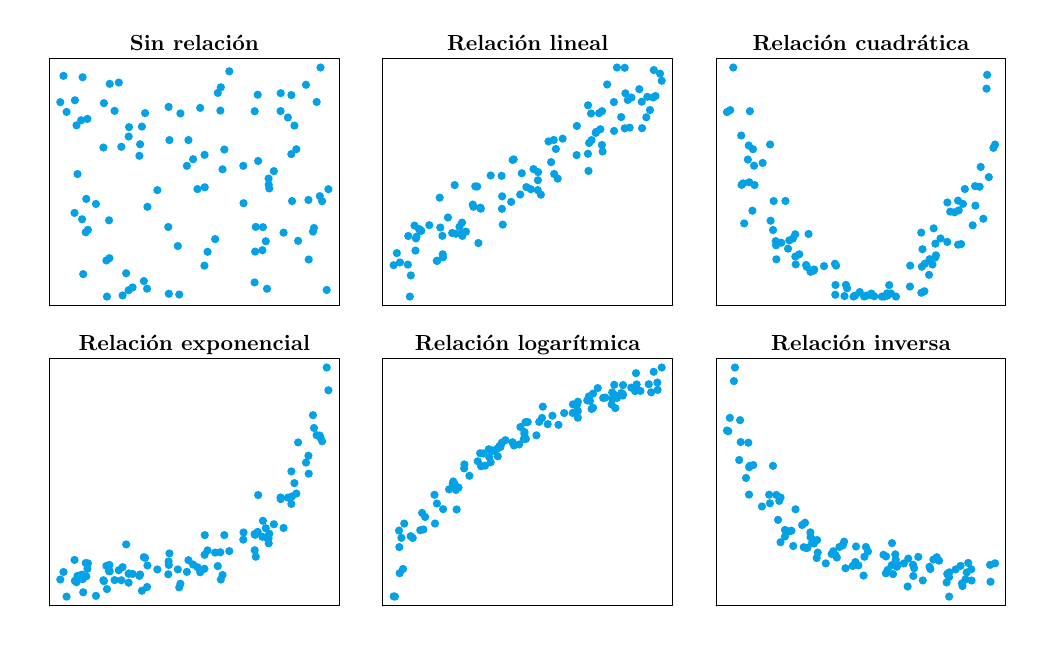
\begin{tikzpicture}[x=1pt,y=1pt]
\definecolor{fillColor}{RGB}{255,255,255}
\path[use as bounding box,fill=fillColor,fill opacity=0.00] (0,0) rectangle (361.35,216.81);
\begin{scope}
\path[clip] (  7.92,116.33) rectangle (112.53,205.72);
\definecolor{fillColor}{RGB}{5,161,230}

\path[fill=fillColor] (100.57,196.18) circle (  1.49);

\path[fill=fillColor] ( 63.92,170.85) circle (  1.49);

\path[fill=fillColor] ( 67.74,140.41) circle (  1.49);

\path[fill=fillColor] ( 43.15,122.50) circle (  1.49);

\path[fill=fillColor] ( 72.86,201.04) circle (  1.49);

\path[fill=fillColor] ( 92.47,142.73) circle (  1.49);

\path[fill=fillColor] ( 29.40,147.19) circle (  1.49);

\path[fill=fillColor] ( 55.18,185.82) circle (  1.49);

\path[fill=fillColor] ( 95.28,171.12) circle (  1.49);

\path[fill=fillColor] ( 27.55,189.53) circle (  1.49);

\path[fill=fillColor] (106.40,154.10) circle (  1.49);

\path[fill=fillColor] ( 94.02,184.36) circle (  1.49);

\path[fill=fillColor] ( 78.01,153.38) circle (  1.49);

\path[fill=fillColor] ( 71.06,172.78) circle (  1.49);

\path[fill=fillColor] ( 34.31,120.06) circle (  1.49);

\path[fill=fillColor] ( 42.42,185.93) circle (  1.49);

\path[fill=fillColor] ( 31.40,186.76) circle (  1.49);

\path[fill=fillColor] ( 41.28,181.07) circle (  1.49);

\path[fill=fillColor] ( 50.81,144.79) circle (  1.49);

\path[fill=fillColor] ( 43.28,152.08) circle (  1.49);

\path[fill=fillColor] ( 68.69,193.23) circle (  1.49);

\path[fill=fillColor] ( 91.38,186.67) circle (  1.49);

\path[fill=fillColor] ( 88.95,164.97) circle (  1.49);

\path[fill=fillColor] ( 87.05,162.28) circle (  1.49);

\path[fill=fillColor] ( 40.63,174.67) circle (  1.49);

\path[fill=fillColor] ( 40.38,170.52) circle (  1.49);

\path[fill=fillColor] (103.46,144.43) circle (  1.49);

\path[fill=fillColor] (104.42,189.97) circle (  1.49);

\path[fill=fillColor] ( 50.93,188.18) circle (  1.49);

\path[fill=fillColor] ( 82.03,186.61) circle (  1.49);

\path[fill=fillColor] (108.06,122.02) circle (  1.49);

\path[fill=fillColor] ( 46.86,158.10) circle (  1.49);

\path[fill=fillColor] ( 77.91,166.90) circle (  1.49);

\path[fill=fillColor] ( 62.33,187.82) circle (  1.49);

\path[fill=fillColor] ( 69.79,195.26) circle (  1.49);

\path[fill=fillColor] ( 97.73,139.78) circle (  1.49);

\path[fill=fillColor] ( 85.00,144.73) circle (  1.49);

\path[fill=fillColor] ( 17.65,181.52) circle (  1.49);

\path[fill=fillColor] (105.81,202.41) circle (  1.49);

\path[fill=fillColor] ( 82.00,124.76) circle (  1.49);

\path[fill=fillColor] ( 35.59,128.06) circle (  1.49);

\path[fill=fillColor] ( 17.06,190.57) circle (  1.49);

\path[fill=fillColor] ( 82.20,135.89) circle (  1.49);

\path[fill=fillColor] ( 86.48,122.46) circle (  1.49);

\path[fill=fillColor] ( 83.29,168.64) circle (  1.49);

\path[fill=fillColor] ( 32.92,196.97) circle (  1.49);

\path[fill=fillColor] ( 87.10,160.06) circle (  1.49);

\path[fill=fillColor] ( 14.06,186.37) circle (  1.49);

\path[fill=fillColor] ( 33.85,173.77) circle (  1.49);

\path[fill=fillColor] ( 69.63,186.84) circle (  1.49);

\path[fill=fillColor] ( 96.39,181.42) circle (  1.49);

\path[fill=fillColor] ( 63.86,130.81) circle (  1.49);

\path[fill=fillColor] ( 57.52,166.88) circle (  1.49);

\path[fill=fillColor] ( 24.68,153.11) circle (  1.49);

\path[fill=fillColor] ( 63.99,159.13) circle (  1.49);

\path[fill=fillColor] ( 12.95,199.40) circle (  1.49);

\path[fill=fillColor] ( 19.85,198.89) circle (  1.49);

\path[fill=fillColor] ( 61.34,158.48) circle (  1.49);

\path[fill=fillColor] ( 28.65,119.64) circle (  1.49);

\path[fill=fillColor] ( 16.93,149.87) circle (  1.49);

\path[fill=fillColor] ( 51.22,176.18) circle (  1.49);

\path[fill=fillColor] ( 37.91,122.94) circle (  1.49);

\path[fill=fillColor] ( 36.46,121.93) circle (  1.49);

\path[fill=fillColor] ( 54.77,120.38) circle (  1.49);

\path[fill=fillColor] (105.57,155.93) circle (  1.49);

\path[fill=fillColor] ( 29.64,196.51) circle (  1.49);

\path[fill=fillColor] ( 65.00,135.82) circle (  1.49);

\path[fill=fillColor] ( 51.00,120.67) circle (  1.49);

\path[fill=fillColor] (108.66,158.44) circle (  1.49);

\path[fill=fillColor] ( 21.18,154.93) circle (  1.49);

\path[fill=fillColor] ( 58.09,176.19) circle (  1.49);

\path[fill=fillColor] ( 20.07,127.75) circle (  1.49);

\path[fill=fillColor] ( 28.44,132.70) circle (  1.49);

\path[fill=fillColor] ( 95.29,192.45) circle (  1.49);

\path[fill=fillColor] ( 27.37,173.50) circle (  1.49);

\path[fill=fillColor] ( 18.01,163.92) circle (  1.49);

\path[fill=fillColor] ( 11.79,189.89) circle (  1.49);

\path[fill=fillColor] ( 20.98,142.88) circle (  1.49);

\path[fill=fillColor] ( 21.58,183.85) circle (  1.49);

\path[fill=fillColor] ( 29.53,133.51) circle (  1.49);

\path[fill=fillColor] ( 70.41,165.63) circle (  1.49);

\path[fill=fillColor] ( 59.77,169.28) circle (  1.49);

\path[fill=fillColor] ( 19.34,183.35) circle (  1.49);

\path[fill=fillColor] ( 82.43,144.82) circle (  1.49);

\path[fill=fillColor] ( 41.98,125.24) circle (  1.49);

\path[fill=fillColor] ( 86.04,139.63) circle (  1.49);

\path[fill=fillColor] (103.09,143.11) circle (  1.49);

\path[fill=fillColor] ( 83.12,192.58) circle (  1.49);

\path[fill=fillColor] ( 87.30,158.72) circle (  1.49);

\path[fill=fillColor] ( 21.77,143.75) circle (  1.49);

\path[fill=fillColor] (101.45,154.56) circle (  1.49);

\path[fill=fillColor] ( 95.54,154.15) circle (  1.49);

\path[fill=fillColor] ( 36.50,177.47) circle (  1.49);

\path[fill=fillColor] ( 91.43,193.13) circle (  1.49);

\path[fill=fillColor] ( 84.81,136.38) circle (  1.49);

\path[fill=fillColor] ( 36.63,180.87) circle (  1.49);

\path[fill=fillColor] (101.55,133.04) circle (  1.49);

\path[fill=fillColor] ( 97.07,172.88) circle (  1.49);

\path[fill=fillColor] ( 54.26,137.90) circle (  1.49);

\path[fill=fillColor] ( 19.67,147.57) circle (  1.49);
\end{scope}
\begin{scope}
\path[clip] (  0.00,108.41) rectangle (120.45,216.81);
\definecolor{drawColor}{RGB}{0,0,0}

\node[text=drawColor,anchor=base,inner sep=0pt, outer sep=0pt, scale=  0.79] at ( 60.22,208.50) {\bfseries Sin relación};

\node[text=drawColor,anchor=base,inner sep=0pt, outer sep=0pt, scale=  0.66] at ( 60.22, 86.23) {$X$};
\end{scope}
\begin{scope}
\path[clip] (  0.00,  0.00) rectangle (361.35,216.81);
\definecolor{drawColor}{RGB}{0,0,0}

\path[draw=drawColor,line width= 0.4pt,line join=round,line cap=round] (  7.92,116.33) --
	(112.53,116.33) --
	(112.53,205.72) --
	(  7.92,205.72) --
	(  7.92,116.33);
\end{scope}
\begin{scope}
\path[clip] (128.37,116.33) rectangle (232.98,205.72);
\definecolor{fillColor}{RGB}{5,161,230}

\path[fill=fillColor] (221.02,194.57) circle (  1.49);

\path[fill=fillColor] (184.37,161.67) circle (  1.49);

\path[fill=fillColor] (188.19,175.70) circle (  1.49);

\path[fill=fillColor] (163.60,151.76) circle (  1.49);

\path[fill=fillColor] (193.31,176.70) circle (  1.49);

\path[fill=fillColor] (212.92,202.41) circle (  1.49);

\path[fill=fillColor] (149.85,141.58) circle (  1.49);

\path[fill=fillColor] (175.63,169.22) circle (  1.49);

\path[fill=fillColor] (215.73,202.31) circle (  1.49);

\path[fill=fillColor] (148.00,132.56) circle (  1.49);

\path[fill=fillColor] (226.85,192.11) circle (  1.49);

\path[fill=fillColor] (214.47,184.51) circle (  1.49);

\path[fill=fillColor] (198.46,181.30) circle (  1.49);

\path[fill=fillColor] (191.51,162.26) circle (  1.49);

\path[fill=fillColor] (154.76,142.34) circle (  1.49);

\path[fill=fillColor] (162.87,138.99) circle (  1.49);

\path[fill=fillColor] (151.85,148.21) circle (  1.49);

\path[fill=fillColor] (161.73,159.47) circle (  1.49);

\path[fill=fillColor] (171.26,163.26) circle (  1.49);

\path[fill=fillColor] (163.73,151.39) circle (  1.49);

\path[fill=fillColor] (189.14,168.22) circle (  1.49);

\path[fill=fillColor] (211.83,189.92) circle (  1.49);

\path[fill=fillColor] (209.40,196.30) circle (  1.49);

\path[fill=fillColor] (207.50,174.41) circle (  1.49);

\path[fill=fillColor] (161.08,152.08) circle (  1.49);

\path[fill=fillColor] (160.83,152.88) circle (  1.49);

\path[fill=fillColor] (223.91,191.82) circle (  1.49);

\path[fill=fillColor] (224.87,187.05) circle (  1.49);

\path[fill=fillColor] (171.38,151.35) circle (  1.49);

\path[fill=fillColor] (202.48,188.77) circle (  1.49);

\path[fill=fillColor] (228.51,200.19) circle (  1.49);

\path[fill=fillColor] (167.31,163.40) circle (  1.49);

\path[fill=fillColor] (198.36,170.76) circle (  1.49);

\path[fill=fillColor] (182.78,165.71) circle (  1.49);

\path[fill=fillColor] (190.24,163.94) circle (  1.49);

\path[fill=fillColor] (218.18,191.55) circle (  1.49);

\path[fill=fillColor] (205.45,179.17) circle (  1.49);

\path[fill=fillColor] (138.10,119.64) circle (  1.49);

\path[fill=fillColor] (226.26,201.49) circle (  1.49);

\path[fill=fillColor] (202.45,171.26) circle (  1.49);

\path[fill=fillColor] (156.04,144.86) circle (  1.49);

\path[fill=fillColor] (137.51,141.53) circle (  1.49);

\path[fill=fillColor] (202.65,165.05) circle (  1.49);

\path[fill=fillColor] (206.93,180.10) circle (  1.49);

\path[fill=fillColor] (203.74,176.17) circle (  1.49);

\path[fill=fillColor] (153.37,142.62) circle (  1.49);

\path[fill=fillColor] (207.55,186.64) circle (  1.49);

\path[fill=fillColor] (134.51,131.97) circle (  1.49);

\path[fill=fillColor] (154.30,159.93) circle (  1.49);

\path[fill=fillColor] (190.08,176.23) circle (  1.49);

\path[fill=fillColor] (216.84,190.68) circle (  1.49);

\path[fill=fillColor] (184.31,158.11) circle (  1.49);

\path[fill=fillColor] (177.97,156.52) circle (  1.49);

\path[fill=fillColor] (145.13,145.44) circle (  1.49);

\path[fill=fillColor] (184.44,164.62) circle (  1.49);

\path[fill=fillColor] (133.40,135.35) circle (  1.49);

\path[fill=fillColor] (140.30,140.66) circle (  1.49);

\path[fill=fillColor] (181.79,158.44) circle (  1.49);

\path[fill=fillColor] (149.10,144.59) circle (  1.49);

\path[fill=fillColor] (137.38,131.19) circle (  1.49);

\path[fill=fillColor] (171.67,145.64) circle (  1.49);

\path[fill=fillColor] (158.36,143.10) circle (  1.49);

\path[fill=fillColor] (156.91,142.27) circle (  1.49);

\path[fill=fillColor] (175.22,169.00) circle (  1.49);

\path[fill=fillColor] (226.02,191.60) circle (  1.49);

\path[fill=fillColor] (150.09,133.85) circle (  1.49);

\path[fill=fillColor] (185.45,156.46) circle (  1.49);

\path[fill=fillColor] (171.45,155.87) circle (  1.49);

\path[fill=fillColor] (229.11,197.62) circle (  1.49);

\path[fill=fillColor] (141.63,143.87) circle (  1.49);

\path[fill=fillColor] (178.54,164.20) circle (  1.49);

\path[fill=fillColor] (140.52,141.26) circle (  1.49);

\path[fill=fillColor] (148.89,155.38) circle (  1.49);

\path[fill=fillColor] (215.74,180.43) circle (  1.49);

\path[fill=fillColor] (147.82,132.55) circle (  1.49);

\path[fill=fillColor] (138.46,127.29) circle (  1.49);

\path[fill=fillColor] (132.24,130.99) circle (  1.49);

\path[fill=fillColor] (141.43,144.00) circle (  1.49);

\path[fill=fillColor] (142.03,143.48) circle (  1.49);

\path[fill=fillColor] (149.98,134.92) circle (  1.49);

\path[fill=fillColor] (190.86,172.98) circle (  1.49);

\path[fill=fillColor] (180.22,159.20) circle (  1.49);

\path[fill=fillColor] (139.79,145.29) circle (  1.49);

\path[fill=fillColor] (202.88,175.15) circle (  1.49);

\path[fill=fillColor] (162.43,159.39) circle (  1.49);

\path[fill=fillColor] (206.49,185.92) circle (  1.49);

\path[fill=fillColor] (223.54,184.43) circle (  1.49);

\path[fill=fillColor] (203.57,185.81) circle (  1.49);

\path[fill=fillColor] (207.75,172.08) circle (  1.49);

\path[fill=fillColor] (142.22,143.38) circle (  1.49);

\path[fill=fillColor] (221.90,190.05) circle (  1.49);

\path[fill=fillColor] (215.99,193.08) circle (  1.49);

\path[fill=fillColor] (156.95,146.38) circle (  1.49);

\path[fill=fillColor] (211.88,179.49) circle (  1.49);

\path[fill=fillColor] (205.26,178.78) circle (  1.49);

\path[fill=fillColor] (157.08,141.56) circle (  1.49);

\path[fill=fillColor] (222.00,180.49) circle (  1.49);

\path[fill=fillColor] (217.52,180.69) circle (  1.49);

\path[fill=fillColor] (174.71,153.86) circle (  1.49);

\path[fill=fillColor] (140.12,136.26) circle (  1.49);
\end{scope}
\begin{scope}
\path[clip] (120.45,108.41) rectangle (240.90,216.81);
\definecolor{drawColor}{RGB}{0,0,0}

\node[text=drawColor,anchor=base,inner sep=0pt, outer sep=0pt, scale=  0.79] at (180.68,208.50) {\bfseries Relación lineal};

\node[text=drawColor,anchor=base,inner sep=0pt, outer sep=0pt, scale=  0.66] at (180.68, 86.23) {$X$};

\node[text=drawColor,rotate= 90.00,anchor=base,inner sep=0pt, outer sep=0pt, scale=  0.66] at (103.03,161.02) {$Y$};
\end{scope}
\begin{scope}
\path[clip] (  0.00,  0.00) rectangle (361.35,216.81);
\definecolor{drawColor}{RGB}{0,0,0}

\path[draw=drawColor,line width= 0.4pt,line join=round,line cap=round] (128.37,116.33) --
	(232.98,116.33) --
	(232.98,205.72) --
	(128.37,205.72) --
	(128.37,116.33);
\end{scope}
\begin{scope}
\path[clip] (248.82,116.33) rectangle (353.43,205.72);
\definecolor{fillColor}{RGB}{5,161,230}

\path[fill=fillColor] (341.47,145.38) circle (  1.49);

\path[fill=fillColor] (304.82,120.43) circle (  1.49);

\path[fill=fillColor] (308.64,119.64) circle (  1.49);

\path[fill=fillColor] (284.05,129.03) circle (  1.49);

\path[fill=fillColor] (313.76,119.64) circle (  1.49);

\path[fill=fillColor] (333.37,150.33) circle (  1.49);

\path[fill=fillColor] (270.30,139.67) circle (  1.49);

\path[fill=fillColor] (296.08,122.65) circle (  1.49);

\path[fill=fillColor] (336.18,154.32) circle (  1.49);

\path[fill=fillColor] (268.45,147.06) circle (  1.49);

\path[fill=fillColor] (347.30,162.81) circle (  1.49);

\path[fill=fillColor] (334.92,150.08) circle (  1.49);

\path[fill=fillColor] (318.91,130.83) circle (  1.49);

\path[fill=fillColor] (311.96,120.75) circle (  1.49);

\path[fill=fillColor] (275.21,139.94) circle (  1.49);

\path[fill=fillColor] (283.32,128.85) circle (  1.49);

\path[fill=fillColor] (272.30,139.11) circle (  1.49);

\path[fill=fillColor] (282.18,142.26) circle (  1.49);

\path[fill=fillColor] (291.71,131.49) circle (  1.49);

\path[fill=fillColor] (284.18,129.42) circle (  1.49);

\path[fill=fillColor] (309.59,119.65) circle (  1.49);

\path[fill=fillColor] (332.28,139.39) circle (  1.49);

\path[fill=fillColor] (329.85,140.64) circle (  1.49);

\path[fill=fillColor] (327.95,133.78) circle (  1.49);

\path[fill=fillColor] (281.53,130.38) circle (  1.49);

\path[fill=fillColor] (281.28,131.05) circle (  1.49);

\path[fill=fillColor] (344.36,166.49) circle (  1.49);

\path[fill=fillColor] (345.32,147.77) circle (  1.49);

\path[fill=fillColor] (291.83,120.30) circle (  1.49);

\path[fill=fillColor] (322.93,121.02) circle (  1.49);

\path[fill=fillColor] (348.96,173.38) circle (  1.49);

\path[fill=fillColor] (287.76,130.66) circle (  1.49);

\path[fill=fillColor] (318.81,123.26) circle (  1.49);

\path[fill=fillColor] (303.23,120.03) circle (  1.49);

\path[fill=fillColor] (310.69,120.02) circle (  1.49);

\path[fill=fillColor] (338.63,158.49) circle (  1.49);

\path[fill=fillColor] (325.90,133.14) circle (  1.49);

\path[fill=fillColor] (258.55,160.55) circle (  1.49);

\path[fill=fillColor] (346.71,199.76) circle (  1.49);

\path[fill=fillColor] (322.90,142.75) circle (  1.49);

\path[fill=fillColor] (276.49,140.57) circle (  1.49);

\path[fill=fillColor] (257.96,159.99) circle (  1.49);

\path[fill=fillColor] (323.10,130.43) circle (  1.49);

\path[fill=fillColor] (327.38,144.29) circle (  1.49);

\path[fill=fillColor] (324.19,131.53) circle (  1.49);

\path[fill=fillColor] (273.82,154.19) circle (  1.49);

\path[fill=fillColor] (328.00,138.75) circle (  1.49);

\path[fill=fillColor] (254.96,202.41) circle (  1.49);

\path[fill=fillColor] (274.75,136.95) circle (  1.49);

\path[fill=fillColor] (310.53,120.80) circle (  1.49);

\path[fill=fillColor] (337.29,138.60) circle (  1.49);

\path[fill=fillColor] (304.76,120.24) circle (  1.49);

\path[fill=fillColor] (298.42,119.64) circle (  1.49);

\path[fill=fillColor] (265.58,167.92) circle (  1.49);

\path[fill=fillColor] (304.89,120.72) circle (  1.49);

\path[fill=fillColor] (253.85,187.01) circle (  1.49);

\path[fill=fillColor] (260.75,160.92) circle (  1.49);

\path[fill=fillColor] (302.24,119.66) circle (  1.49);

\path[fill=fillColor] (269.55,154.17) circle (  1.49);

\path[fill=fillColor] (257.83,177.84) circle (  1.49);

\path[fill=fillColor] (292.12,130.83) circle (  1.49);

\path[fill=fillColor] (278.81,134.91) circle (  1.49);

\path[fill=fillColor] (277.36,142.15) circle (  1.49);

\path[fill=fillColor] (295.67,123.86) circle (  1.49);

\path[fill=fillColor] (346.47,194.78) circle (  1.49);

\path[fill=fillColor] (270.54,133.10) circle (  1.49);

\path[fill=fillColor] (305.90,119.77) circle (  1.49);

\path[fill=fillColor] (291.90,123.83) circle (  1.49);

\path[fill=fillColor] (349.56,174.57) circle (  1.49);

\path[fill=fillColor] (262.08,172.89) circle (  1.49);

\path[fill=fillColor] (298.99,119.99) circle (  1.49);

\path[fill=fillColor] (260.97,186.63) circle (  1.49);

\path[fill=fillColor] (269.34,143.69) circle (  1.49);

\path[fill=fillColor] (336.19,138.40) circle (  1.49);

\path[fill=fillColor] (268.27,174.60) circle (  1.49);

\path[fill=fillColor] (258.91,146.08) circle (  1.49);

\path[fill=fillColor] (252.69,186.31) circle (  1.49);

\path[fill=fillColor] (261.88,150.67) circle (  1.49);

\path[fill=fillColor] (262.48,166.93) circle (  1.49);

\path[fill=fillColor] (270.43,138.17) circle (  1.49);

\path[fill=fillColor] (311.31,123.77) circle (  1.49);

\path[fill=fillColor] (300.67,121.29) circle (  1.49);

\path[fill=fillColor] (260.24,169.15) circle (  1.49);

\path[fill=fillColor] (323.33,136.75) circle (  1.49);

\path[fill=fillColor] (282.88,128.60) circle (  1.49);

\path[fill=fillColor] (326.94,131.24) circle (  1.49);

\path[fill=fillColor] (343.99,159.33) circle (  1.49);

\path[fill=fillColor] (324.02,121.56) circle (  1.49);

\path[fill=fillColor] (328.20,134.54) circle (  1.49);

\path[fill=fillColor] (262.67,159.93) circle (  1.49);

\path[fill=fillColor] (342.35,159.55) circle (  1.49);

\path[fill=fillColor] (336.44,150.78) circle (  1.49);

\path[fill=fillColor] (277.40,134.12) circle (  1.49);

\path[fill=fillColor] (332.33,153.64) circle (  1.49);

\path[fill=fillColor] (325.71,127.51) circle (  1.49);

\path[fill=fillColor] (277.53,131.27) circle (  1.49);

\path[fill=fillColor] (342.45,152.50) circle (  1.49);

\path[fill=fillColor] (337.97,153.12) circle (  1.49);

\path[fill=fillColor] (295.16,119.83) circle (  1.49);

\path[fill=fillColor] (260.57,174.22) circle (  1.49);
\end{scope}
\begin{scope}
\path[clip] (240.90,108.41) rectangle (361.35,216.81);
\definecolor{drawColor}{RGB}{0,0,0}

\node[text=drawColor,anchor=base,inner sep=0pt, outer sep=0pt, scale=  0.79] at (301.12,208.50) {\bfseries Relación cuadrática};

\node[text=drawColor,anchor=base,inner sep=0pt, outer sep=0pt, scale=  0.66] at (301.12, 86.23) {$X$};

\node[text=drawColor,rotate= 90.00,anchor=base,inner sep=0pt, outer sep=0pt, scale=  0.66] at (223.48,161.02) {$Y$};
\end{scope}
\begin{scope}
\path[clip] (  0.00,  0.00) rectangle (361.35,216.81);
\definecolor{drawColor}{RGB}{0,0,0}

\path[draw=drawColor,line width= 0.4pt,line join=round,line cap=round] (248.82,116.33) --
	(353.43,116.33) --
	(353.43,205.72) --
	(248.82,205.72) --
	(248.82,116.33);
\end{scope}
\begin{scope}
\path[clip] (  7.92,  7.92) rectangle (112.53, 97.32);
\definecolor{fillColor}{RGB}{5,161,230}

\path[fill=fillColor] (100.57, 59.65) circle (  1.49);

\path[fill=fillColor] ( 63.92, 26.33) circle (  1.49);

\path[fill=fillColor] ( 67.74, 27.13) circle (  1.49);

\path[fill=fillColor] ( 43.15, 14.70) circle (  1.49);

\path[fill=fillColor] ( 72.86, 27.67) circle (  1.49);

\path[fill=fillColor] ( 92.47, 36.03) circle (  1.49);

\path[fill=fillColor] ( 29.40, 20.42) circle (  1.49);

\path[fill=fillColor] ( 55.18, 15.87) circle (  1.49);

\path[fill=fillColor] ( 95.28, 44.72) circle (  1.49);

\path[fill=fillColor] ( 27.55, 16.81) circle (  1.49);

\path[fill=fillColor] (106.40, 67.35) circle (  1.49);

\path[fill=fillColor] ( 94.02, 47.01) circle (  1.49);

\path[fill=fillColor] ( 78.01, 34.41) circle (  1.49);

\path[fill=fillColor] ( 71.06, 33.45) circle (  1.49);

\path[fill=fillColor] ( 34.31, 21.87) circle (  1.49);

\path[fill=fillColor] ( 42.42, 25.23) circle (  1.49);

\path[fill=fillColor] ( 31.40, 17.19) circle (  1.49);

\path[fill=fillColor] ( 41.28, 13.34) circle (  1.49);

\path[fill=fillColor] ( 50.81, 19.29) circle (  1.49);

\path[fill=fillColor] ( 43.28, 22.47) circle (  1.49);

\path[fill=fillColor] ( 68.69, 22.26) circle (  1.49);

\path[fill=fillColor] ( 91.38, 47.04) circle (  1.49);

\path[fill=fillColor] ( 88.95, 37.37) circle (  1.49);

\path[fill=fillColor] ( 87.05, 32.35) circle (  1.49);

\path[fill=fillColor] ( 40.63, 19.22) circle (  1.49);

\path[fill=fillColor] ( 40.38, 18.72) circle (  1.49);

\path[fill=fillColor] (103.46, 72.16) circle (  1.49);

\path[fill=fillColor] (104.42, 69.55) circle (  1.49);

\path[fill=fillColor] ( 50.93, 23.95) circle (  1.49);

\path[fill=fillColor] ( 82.03, 27.98) circle (  1.49);

\path[fill=fillColor] (108.06, 94.01) circle (  1.49);

\path[fill=fillColor] ( 46.86, 21.04) circle (  1.49);

\path[fill=fillColor] ( 77.91, 31.81) circle (  1.49);

\path[fill=fillColor] ( 62.33, 20.03) circle (  1.49);

\path[fill=fillColor] ( 69.79, 17.40) circle (  1.49);

\path[fill=fillColor] ( 97.73, 66.94) circle (  1.49);

\path[fill=fillColor] ( 85.00, 38.61) circle (  1.49);

\path[fill=fillColor] ( 17.65, 16.42) circle (  1.49);

\path[fill=fillColor] (105.81, 68.63) circle (  1.49);

\path[fill=fillColor] ( 82.00, 33.81) circle (  1.49);

\path[fill=fillColor] ( 35.59, 30.09) circle (  1.49);

\path[fill=fillColor] ( 17.06, 16.91) circle (  1.49);

\path[fill=fillColor] ( 82.20, 33.54) circle (  1.49);

\path[fill=fillColor] ( 86.48, 32.40) circle (  1.49);

\path[fill=fillColor] ( 83.29, 47.92) circle (  1.49);

\path[fill=fillColor] ( 32.92, 20.77) circle (  1.49);

\path[fill=fillColor] ( 87.10, 30.48) circle (  1.49);

\path[fill=fillColor] ( 14.06, 11.23) circle (  1.49);

\path[fill=fillColor] ( 33.85, 17.14) circle (  1.49);

\path[fill=fillColor] ( 69.63, 27.24) circle (  1.49);

\path[fill=fillColor] ( 96.39, 52.23) circle (  1.49);

\path[fill=fillColor] ( 63.86, 21.28) circle (  1.49);

\path[fill=fillColor] ( 57.52, 20.16) circle (  1.49);

\path[fill=fillColor] ( 24.68, 11.50) circle (  1.49);

\path[fill=fillColor] ( 63.99, 33.44) circle (  1.49);

\path[fill=fillColor] ( 12.95, 20.12) circle (  1.49);

\path[fill=fillColor] ( 19.85, 17.53) circle (  1.49);

\path[fill=fillColor] ( 61.34, 21.85) circle (  1.49);

\path[fill=fillColor] ( 28.65, 13.94) circle (  1.49);

\path[fill=fillColor] ( 16.93, 24.48) circle (  1.49);

\path[fill=fillColor] ( 51.22, 26.84) circle (  1.49);

\path[fill=fillColor] ( 37.91, 19.41) circle (  1.49);

\path[fill=fillColor] ( 36.46, 16.26) circle (  1.49);

\path[fill=fillColor] ( 54.77, 14.57) circle (  1.49);

\path[fill=fillColor] (105.57, 69.41) circle (  1.49);

\path[fill=fillColor] ( 29.64, 20.37) circle (  1.49);

\path[fill=fillColor] ( 65.00, 27.93) circle (  1.49);

\path[fill=fillColor] ( 51.00, 22.67) circle (  1.49);

\path[fill=fillColor] (108.66, 85.78) circle (  1.49);

\path[fill=fillColor] ( 21.18, 18.54) circle (  1.49);

\path[fill=fillColor] ( 58.09, 24.37) circle (  1.49);

\path[fill=fillColor] ( 20.07, 12.79) circle (  1.49);

\path[fill=fillColor] ( 28.44, 22.34) circle (  1.49);

\path[fill=fillColor] ( 95.29, 56.47) circle (  1.49);

\path[fill=fillColor] ( 27.37, 17.14) circle (  1.49);

\path[fill=fillColor] ( 18.01, 18.72) circle (  1.49);

\path[fill=fillColor] ( 11.79, 17.40) circle (  1.49);

\path[fill=fillColor] ( 20.98, 23.36) circle (  1.49);

\path[fill=fillColor] ( 21.58, 21.27) circle (  1.49);

\path[fill=fillColor] ( 29.53, 22.67) circle (  1.49);

\path[fill=fillColor] ( 70.41, 19.04) circle (  1.49);

\path[fill=fillColor] ( 59.77, 22.81) circle (  1.49);

\path[fill=fillColor] ( 19.34, 19.04) circle (  1.49);

\path[fill=fillColor] ( 82.43, 25.64) circle (  1.49);

\path[fill=fillColor] ( 41.98, 25.47) circle (  1.49);

\path[fill=fillColor] ( 86.04, 35.93) circle (  1.49);

\path[fill=fillColor] (103.09, 76.78) circle (  1.49);

\path[fill=fillColor] ( 83.12, 34.61) circle (  1.49);

\path[fill=fillColor] ( 87.30, 33.92) circle (  1.49);

\path[fill=fillColor] ( 21.77, 23.24) circle (  1.49);

\path[fill=fillColor] (101.45, 62.12) circle (  1.49);

\path[fill=fillColor] ( 95.54, 47.43) circle (  1.49);

\path[fill=fillColor] ( 36.50, 19.48) circle (  1.49);

\path[fill=fillColor] ( 91.43, 46.47) circle (  1.49);

\path[fill=fillColor] ( 84.81, 32.84) circle (  1.49);

\path[fill=fillColor] ( 36.63, 19.56) circle (  1.49);

\path[fill=fillColor] (101.55, 55.64) circle (  1.49);

\path[fill=fillColor] ( 97.07, 48.47) circle (  1.49);

\path[fill=fillColor] ( 54.26, 21.04) circle (  1.49);

\path[fill=fillColor] ( 19.67, 19.15) circle (  1.49);
\end{scope}
\begin{scope}
\path[clip] (  0.00,  0.00) rectangle (120.45,108.41);
\definecolor{drawColor}{RGB}{0,0,0}

\node[text=drawColor,anchor=base,inner sep=0pt, outer sep=0pt, scale=  0.79] at ( 60.22,100.09) {\bfseries Relación exponencial};
\end{scope}
\begin{scope}
\path[clip] (  0.00,  0.00) rectangle (361.35,216.81);
\definecolor{drawColor}{RGB}{0,0,0}

\path[draw=drawColor,line width= 0.4pt,line join=round,line cap=round] (  7.92,  7.92) --
	(112.53,  7.92) --
	(112.53, 97.32) --
	(  7.92, 97.32) --
	(  7.92,  7.92);
\end{scope}
\begin{scope}
\path[clip] (128.37,  7.92) rectangle (232.98, 97.32);
\definecolor{fillColor}{RGB}{5,161,230}

\path[fill=fillColor] (166.79, 61.64) circle (  1.49);

\path[fill=fillColor] (153.61, 52.04) circle (  1.49);

\path[fill=fillColor] (227.52, 88.58) circle (  1.49);

\path[fill=fillColor] (225.29, 85.05) circle (  1.49);

\path[fill=fillColor] (143.62, 40.01) circle (  1.49);

\path[fill=fillColor] (185.85, 75.79) circle (  1.49);

\path[fill=fillColor] (134.43, 19.68) circle (  1.49);

\path[fill=fillColor] (211.21, 85.02) circle (  1.49);

\path[fill=fillColor] (179.53, 70.69) circle (  1.49);

\path[fill=fillColor] (211.25, 82.67) circle (  1.49);

\path[fill=fillColor] (164.70, 62.95) circle (  1.49);

\path[fill=fillColor] (179.89, 74.28) circle (  1.49);

\path[fill=fillColor] (154.36, 51.77) circle (  1.49);

\path[fill=fillColor] (218.09, 86.74) circle (  1.49);

\path[fill=fillColor] (153.80, 52.82) circle (  1.49);

\path[fill=fillColor] (142.98, 35.48) circle (  1.49);

\path[fill=fillColor] (229.11, 94.01) circle (  1.49);

\path[fill=fillColor] (165.26, 58.54) circle (  1.49);

\path[fill=fillColor] (135.63, 21.22) circle (  1.49);

\path[fill=fillColor] (202.20, 82.14) circle (  1.49);

\path[fill=fillColor] (196.95, 77.59) circle (  1.49);

\path[fill=fillColor] (207.96, 83.03) circle (  1.49);

\path[fill=fillColor] (175.19, 67.01) circle (  1.49);

\path[fill=fillColor] (220.06, 87.91) circle (  1.49);

\path[fill=fillColor] (205.98, 86.57) circle (  1.49);

\path[fill=fillColor] (179.25, 68.12) circle (  1.49);

\path[fill=fillColor] (147.89, 44.85) circle (  1.49);

\path[fill=fillColor] (134.30, 29.12) circle (  1.49);

\path[fill=fillColor] (135.06, 32.45) circle (  1.49);

\path[fill=fillColor] (170.86, 65.32) circle (  1.49);

\path[fill=fillColor] (134.20, 35.09) circle (  1.49);

\path[fill=fillColor] (178.06, 72.51) circle (  1.49);

\path[fill=fillColor] (187.92, 73.54) circle (  1.49);

\path[fill=fillColor] (159.62, 54.88) circle (  1.49);

\path[fill=fillColor] (147.17, 37.63) circle (  1.49);

\path[fill=fillColor] (168.04, 63.99) circle (  1.49);

\path[fill=fillColor] (191.80, 73.30) circle (  1.49);

\path[fill=fillColor] (162.62, 60.12) circle (  1.49);

\path[fill=fillColor] (203.20, 81.93) circle (  1.49);

\path[fill=fillColor] (193.86, 77.55) circle (  1.49);

\path[fill=fillColor] (215.07, 84.37) circle (  1.49);

\path[fill=fillColor] (198.83, 81.64) circle (  1.49);

\path[fill=fillColor] (186.15, 79.87) circle (  1.49);

\path[fill=fillColor] (139.14, 32.42) circle (  1.49);

\path[fill=fillColor] (183.83, 69.50) circle (  1.49);

\path[fill=fillColor] (177.58, 66.21) circle (  1.49);

\path[fill=fillColor] (180.04, 68.23) circle (  1.49);

\path[fill=fillColor] (157.71, 57.58) circle (  1.49);

\path[fill=fillColor] (198.80, 75.87) circle (  1.49);

\path[fill=fillColor] (175.69, 65.85) circle (  1.49);

\path[fill=fillColor] (226.19, 92.46) circle (  1.49);

\path[fill=fillColor] (203.78, 79.02) circle (  1.49);

\path[fill=fillColor] (180.69, 74.30) circle (  1.49);

\path[fill=fillColor] (198.81, 78.26) circle (  1.49);

\path[fill=fillColor] (147.00, 48.02) circle (  1.49);

\path[fill=fillColor] (138.38, 33.06) circle (  1.49);

\path[fill=fillColor] (211.00, 80.67) circle (  1.49);

\path[fill=fillColor] (179.48, 69.99) circle (  1.49);

\path[fill=fillColor] (197.02, 80.69) circle (  1.49);

\path[fill=fillColor] (169.64, 64.62) circle (  1.49);

\path[fill=fillColor] (154.77, 49.77) circle (  1.49);

\path[fill=fillColor] (214.53, 84.80) circle (  1.49);

\path[fill=fillColor] (198.52, 80.75) circle (  1.49);

\path[fill=fillColor] (202.80, 83.57) circle (  1.49);

\path[fill=fillColor] (212.34, 79.34) circle (  1.49);

\path[fill=fillColor] (204.30, 79.44) circle (  1.49);

\path[fill=fillColor] (212.07, 84.09) circle (  1.49);

\path[fill=fillColor] (141.86, 35.22) circle (  1.49);

\path[fill=fillColor] (167.31, 59.77) circle (  1.49);

\path[fill=fillColor] (163.50, 63.03) circle (  1.49);

\path[fill=fillColor] (142.52, 41.46) circle (  1.49);

\path[fill=fillColor] (189.61, 76.60) circle (  1.49);

\path[fill=fillColor] (163.82, 58.36) circle (  1.49);

\path[fill=fillColor] (211.96, 87.76) circle (  1.49);

\path[fill=fillColor] (227.63, 85.92) circle (  1.49);

\path[fill=fillColor] (132.71, 11.23) circle (  1.49);

\path[fill=fillColor] (221.42, 85.54) circle (  1.49);

\path[fill=fillColor] (198.30, 80.24) circle (  1.49);

\path[fill=fillColor] (219.82, 91.96) circle (  1.49);

\path[fill=fillColor] (224.42, 87.97) circle (  1.49);

\path[fill=fillColor] (168.29, 63.80) circle (  1.49);

\path[fill=fillColor] (157.80, 58.99) circle (  1.49);

\path[fill=fillColor] (219.48, 85.49) circle (  1.49);

\path[fill=fillColor] (136.07, 37.61) circle (  1.49);

\path[fill=fillColor] (155.68, 50.62) circle (  1.49);

\path[fill=fillColor] (132.24, 11.31) circle (  1.49);

\path[fill=fillColor] (208.73, 83.14) circle (  1.49);

\path[fill=fillColor] (150.10, 42.82) circle (  1.49);

\path[fill=fillColor] (170.45, 65.55) circle (  1.49);

\path[fill=fillColor] (184.84, 74.37) circle (  1.49);

\path[fill=fillColor] (215.13, 87.66) circle (  1.49);

\path[fill=fillColor] (172.64, 67.74) circle (  1.49);

\path[fill=fillColor] (166.61, 64.47) circle (  1.49);

\path[fill=fillColor] (155.01, 42.71) circle (  1.49);

\path[fill=fillColor] (171.33, 66.84) circle (  1.49);

\path[fill=fillColor] (215.02, 83.87) circle (  1.49);

\path[fill=fillColor] (169.86, 61.92) circle (  1.49);

\path[fill=fillColor] (212.94, 82.98) circle (  1.49);

\path[fill=fillColor] (204.26, 84.57) circle (  1.49);

\path[fill=fillColor] (152.27, 49.99) circle (  1.49);
\end{scope}
\begin{scope}
\path[clip] (120.45,  0.00) rectangle (240.90,108.41);
\definecolor{drawColor}{RGB}{0,0,0}

\node[text=drawColor,anchor=base,inner sep=0pt, outer sep=0pt, scale=  0.79] at (180.68,100.09) {\bfseries Relación logarítmica};

\node[text=drawColor,rotate= 90.00,anchor=base,inner sep=0pt, outer sep=0pt, scale=  0.66] at (103.03, 52.62) {$Y$};
\end{scope}
\begin{scope}
\path[clip] (  0.00,  0.00) rectangle (361.35,216.81);
\definecolor{drawColor}{RGB}{0,0,0}

\path[draw=drawColor,line width= 0.4pt,line join=round,line cap=round] (128.37,  7.92) --
	(232.98,  7.92) --
	(232.98, 97.32) --
	(128.37, 97.32) --
	(128.37,  7.92);
\end{scope}
\begin{scope}
\path[clip] (248.82,  7.92) rectangle (353.43, 97.32);
\definecolor{fillColor}{RGB}{5,161,230}

\path[fill=fillColor] (288.38, 23.23) circle (  1.49);

\path[fill=fillColor] (260.41, 66.84) circle (  1.49);

\path[fill=fillColor] (327.30, 24.62) circle (  1.49);

\path[fill=fillColor] (340.98, 21.10) circle (  1.49);

\path[fill=fillColor] (312.22, 22.57) circle (  1.49);

\path[fill=fillColor] (284.12, 30.42) circle (  1.49);

\path[fill=fillColor] (294.54, 29.74) circle (  1.49);

\path[fill=fillColor] (291.10, 27.61) circle (  1.49);

\path[fill=fillColor] (323.44, 17.07) circle (  1.49);

\path[fill=fillColor] (332.93, 18.25) circle (  1.49);

\path[fill=fillColor] (271.57, 45.81) circle (  1.49);

\path[fill=fillColor] (291.86, 26.29) circle (  1.49);

\path[fill=fillColor] (282.83, 34.45) circle (  1.49);

\path[fill=fillColor] (313.50, 26.49) circle (  1.49);

\path[fill=fillColor] (283.45, 30.70) circle (  1.49);

\path[fill=fillColor] (310.74, 20.87) circle (  1.49);

\path[fill=fillColor] (298.11, 22.30) circle (  1.49);

\path[fill=fillColor] (302.36, 25.63) circle (  1.49);

\path[fill=fillColor] (299.09, 23.72) circle (  1.49);

\path[fill=fillColor] (255.19, 89.10) circle (  1.49);

\path[fill=fillColor] (252.69, 71.24) circle (  1.49);

\path[fill=fillColor] (312.33, 30.55) circle (  1.49);

\path[fill=fillColor] (270.54, 47.97) circle (  1.49);

\path[fill=fillColor] (332.28, 19.46) circle (  1.49);

\path[fill=fillColor] (318.19, 24.96) circle (  1.49);

\path[fill=fillColor] (337.09, 22.33) circle (  1.49);

\path[fill=fillColor] (337.80, 15.04) circle (  1.49);

\path[fill=fillColor] (326.18, 21.20) circle (  1.49);

\path[fill=fillColor] (281.76, 28.87) circle (  1.49);

\path[fill=fillColor] (253.16, 70.99) circle (  1.49);

\path[fill=fillColor] (260.70, 57.99) circle (  1.49);

\path[fill=fillColor] (285.26, 31.65) circle (  1.49);

\path[fill=fillColor] (317.97, 14.88) circle (  1.49);

\path[fill=fillColor] (314.06, 22.02) circle (  1.49);

\path[fill=fillColor] (273.64, 32.95) circle (  1.49);

\path[fill=fillColor] (269.31, 58.48) circle (  1.49);

\path[fill=fillColor] (257.43, 74.99) circle (  1.49);

\path[fill=fillColor] (290.51, 26.63) circle (  1.49);

\path[fill=fillColor] (260.65, 48.09) circle (  1.49);

\path[fill=fillColor] (329.32, 24.22) circle (  1.49);

\path[fill=fillColor] (274.94, 34.76) circle (  1.49);

\path[fill=fillColor] (332.97, 11.23) circle (  1.49);

\path[fill=fillColor] (320.02, 18.69) circle (  1.49);

\path[fill=fillColor] (265.34, 43.80) circle (  1.49);

\path[fill=fillColor] (295.52, 21.48) circle (  1.49);

\path[fill=fillColor] (333.05, 20.00) circle (  1.49);

\path[fill=fillColor] (349.56, 23.25) circle (  1.49);

\path[fill=fillColor] (276.63, 29.52) circle (  1.49);

\path[fill=fillColor] (257.12, 60.58) circle (  1.49);

\path[fill=fillColor] (335.32, 21.06) circle (  1.49);

\path[fill=fillColor] (295.02, 31.09) circle (  1.49);

\path[fill=fillColor] (316.58, 23.21) circle (  1.49);

\path[fill=fillColor] (285.49, 27.14) circle (  1.49);

\path[fill=fillColor] (268.22, 44.95) circle (  1.49);

\path[fill=fillColor] (302.05, 18.83) circle (  1.49);

\path[fill=fillColor] (262.19, 58.76) circle (  1.49);

\path[fill=fillColor] (284.07, 31.62) circle (  1.49);

\path[fill=fillColor] (253.73, 75.83) circle (  1.49);

\path[fill=fillColor] (325.87, 22.01) circle (  1.49);

\path[fill=fillColor] (281.38, 28.76) circle (  1.49);

\path[fill=fillColor] (292.39, 25.35) circle (  1.49);

\path[fill=fillColor] (347.92, 16.59) circle (  1.49);

\path[fill=fillColor] (321.82, 25.58) circle (  1.49);

\path[fill=fillColor] (277.46, 42.77) circle (  1.49);

\path[fill=fillColor] (312.70, 19.35) circle (  1.49);

\path[fill=fillColor] (267.93, 48.05) circle (  1.49);

\path[fill=fillColor] (280.89, 37.91) circle (  1.49);

\path[fill=fillColor] (280.42, 29.08) circle (  1.49);

\path[fill=fillColor] (260.92, 58.46) circle (  1.49);

\path[fill=fillColor] (313.66, 24.53) circle (  1.49);

\path[fill=fillColor] (271.15, 38.94) circle (  1.49);

\path[fill=fillColor] (320.31, 21.52) circle (  1.49);

\path[fill=fillColor] (300.18, 22.50) circle (  1.49);

\path[fill=fillColor] (332.06, 16.33) circle (  1.49);

\path[fill=fillColor] (310.18, 25.75) circle (  1.49);

\path[fill=fillColor] (285.10, 25.16) circle (  1.49);

\path[fill=fillColor] (341.09, 17.04) circle (  1.49);

\path[fill=fillColor] (328.49, 25.46) circle (  1.49);

\path[fill=fillColor] (337.62, 15.98) circle (  1.49);

\path[fill=fillColor] (339.33, 19.98) circle (  1.49);

\path[fill=fillColor] (339.87, 23.39) circle (  1.49);

\path[fill=fillColor] (310.10, 19.64) circle (  1.49);

\path[fill=fillColor] (299.32, 29.33) circle (  1.49);

\path[fill=fillColor] (257.64, 67.07) circle (  1.49);

\path[fill=fillColor] (279.86, 37.09) circle (  1.49);

\path[fill=fillColor] (255.57, 94.01) circle (  1.49);

\path[fill=fillColor] (272.04, 30.87) circle (  1.49);

\path[fill=fillColor] (293.33, 29.17) circle (  1.49);

\path[fill=fillColor] (302.89, 29.16) circle (  1.49);

\path[fill=fillColor] (314.47, 22.68) circle (  1.49);

\path[fill=fillColor] (275.96, 35.04) circle (  1.49);

\path[fill=fillColor] (338.89, 17.47) circle (  1.49);

\path[fill=fillColor] (272.05, 47.04) circle (  1.49);

\path[fill=fillColor] (319.90, 22.76) circle (  1.49);

\path[fill=fillColor] (347.77, 22.70) circle (  1.49);

\path[fill=fillColor] (259.57, 54.09) circle (  1.49);

\path[fill=fillColor] (303.63, 27.52) circle (  1.49);

\path[fill=fillColor] (273.64, 35.33) circle (  1.49);

\path[fill=fillColor] (282.89, 32.69) circle (  1.49);

\path[fill=fillColor] (309.25, 26.32) circle (  1.49);
\end{scope}
\begin{scope}
\path[clip] (240.90,  0.00) rectangle (361.35,108.41);
\definecolor{drawColor}{RGB}{0,0,0}

\node[text=drawColor,anchor=base,inner sep=0pt, outer sep=0pt, scale=  0.79] at (301.12,100.09) {\bfseries Relación inversa};

\node[text=drawColor,rotate= 90.00,anchor=base,inner sep=0pt, outer sep=0pt, scale=  0.66] at (223.48, 52.62) {$Y$};
\end{scope}
\begin{scope}
\path[clip] (  0.00,  0.00) rectangle (361.35,216.81);
\definecolor{drawColor}{RGB}{0,0,0}

\path[draw=drawColor,line width= 0.4pt,line join=round,line cap=round] (248.82,  7.92) --
	(353.43,  7.92) --
	(353.43, 97.32) --
	(248.82, 97.32) --
	(248.82,  7.92);
\end{scope}
\end{tikzpicture}
}

\note{Dependiendo del tipo de relación entre las variables, la nube de puntos del diagrama de dispersión tendrá distintas formas. Aquí se
presentan algunos ejemplos.

En el primer caso tenemos un diagrama de dispersión de dos variables independientes. En este caso la nube de
puntos no tendrá una forma definida aunque normalmentes los puntos formarán un cúmulo circular.

En el segundo caso tenemos el diagrama de dispersión de dos variables relacionadas linealmente. En este caso la nube de puntos tendrá una
forma más o menos de recta.

En el tercer caso tenemos el diagrama de dispersión de dos variables relacionadas parabólicamente, de forma que la nube de puntos tiene
forma de parábola.

El cuarto caso se corresponde con una relación exponencial, donde la nube de puntos tiene más o menos la forma de una curva exponencial.

El quinto caso corresponde a una relación logarítmica, donde la nube de puntos tiene forma de curva logarítmica.

Y finalmente el último caso correspondería a una relación inversa.}
\end{frame}


%---------------------------------------------------------------------slide----
\begin{frame}
\frametitle{Distribuciones marginales}
A cada una de las distribuciones de las variables que conforman la variable bidimensional se les llama \structure{\textbf{distribuciones marginales}}.

Las distribuciones marginales se pueden obtener a partir de la tabla de frecuencias bidimensional, sumando las frecuencias por filas y columnas.
\begin{center}
\[
\begin{array}{|c|ccccc|>{\columncolor{color1!50}}c|}
\hline
X\backslash Y & y_1 & \cdots & y_j & \cdots & y_q & n_x\\
\hline
x_1 & n_{11} & \cdots & n_{1j} & \cdots & n_{1q} & n_{x_1}\\
\vdots & \vdots & \vdots & \tikz[baseline=-0.5ex]{\node at (0,0) [fill=color2!50,single arrow,shape border
rotate=270, single arrow head extend=1mm]{$+$\phantom{}}; } & \vdots &
\vdots & \vdots \\
x_i & n_{i1} & \tikz[baseline=-0.5ex]{\node at (0,0) [fill=color1!50,single arrow,shape border rotate=0,
single arrow head extend=1mm]{$+$\phantom{}}; }  & n_{ij} & \tikz[baseline=-0.5ex]{\node
at (0,0) [fill=color1!50,single arrow,shape border rotate=0, single
arrow head extend=1mm]{$+$\phantom{}}; } & n_{iq} & n_{x_i}\\
\vdots & \vdots & \vdots & \tikz[baseline=-0.5ex]{\node at (0,0) [fill=color2!50,single arrow,shape border
rotate=270, single arrow head extend=1mm]{$+$\phantom{}}; } & \vdots & \vdots & \vdots\\
x_p & n_{p1} & \cdots & n_{pj} & \cdots & n_{pq} & n_{x_p} \\
\hline
\rowcolor{color2!50}
n_y & n_{y_1} & \cdots & n_{y_j} & \cdots & n_{y_q} & \cellcolor{white} n\\
\hline
\end{array}
\]
\end{center}

\note{A partir de la tabla de frecuencias bidimensional es posible obtener la distribución de frecuencias de cada una de las variables
individuales que componenen la variable bidimensional sumando las frecuencias de la tabla por filas para una de las variables y por columnas
para otra. Por ejemplo, para obtener la frecuencia absoluta de $x_i$ basta sumar las frecuencias absolutas que aparecen en la fila
correspondiente a $x_i$, mientras que para obtener la frecuencia de $y_i$ hay que sumar las frecuencias absolutas que aparecen en la
columna correspondiente a $y_j$. 

Como las distribuciones de cada variable aparecen en los márgenes de la tabla, se les llama distribuciones
marginales.}
\end{frame}


%---------------------------------------------------------------------slide----
\begin{frame}
\frametitle{Distribuciones marginales}
\framesubtitle{Ejemplo con estaturas y pesos}
En el ejemplo anterior de las estaturas y los pesos, las distribuciones marginales son
\[
\begin{array}{|c||c|c|c|c|c|c|>{\columncolor{royalblue1}}c|}
\hline
  X/Y & [50,60) & [60,70) & [70,80) & [80,90) & [90,100) & [100,110) & n_x\\
  \hline\hline
  (150,160] & 2 & 0 & 0 & 0 & 0 & 0 & 2\\
  \hline
  (160,170] & 4 & 4 & 0 & 0 & 0 & 0 & 8\\
  \hline
  (170,180] & 1 & 6 & 3 & 1 & 0 & 0 & 11 \\
  \hline
  (180,190] & 0 & 1 & 4 & 1 & 1 & 0 & 7 \\
  \hline
  (190,200] & 0 & 0 & 0 & 0 & 1 & 1 & 2\\
  \hline
  \rowcolor{coral}
  n_y & 7 & 11 & 7 & 2 & 2 & 1 & \cellcolor{white} 30\\
  \hline
\end{array}
\]
y los estadísticos correspondientes son
\[
\begin{array}{lllll}
\bar x = 174.67 \mbox{ cm} & \quad & s^2_x = 102.06 \mbox{ cm}^2 & \quad & s_x = 10.1 \mbox{ cm}\\
\bar y = 69.67 \mbox{ Kg} & & s^2_y = 164.42 \mbox{ Kg}^2 & & s_y = 12.82 \mbox{ Kg}
\end{array}
\]

\note{En el ejemplo de las estaturas y los pesos, para obtener la distribución marginal de la Estatura, sumamos las frecuencias por filas.
Así, para calcular la frecuencia absoluta del intervalo $(150,160]$ sumamos las frecuencias de su fila ya que todas esas personas miden
entre 150 y 160 cm, es decir, 2 + 0 + 0 etc., lo que nos da 2. La frecuencia absoluta del intervalo $(160,170]$ es 4 + 4 + 0 etc. lo que
nos da 8 y así sucesivamente.

Por otro lado, para obtener la distribución marginal del peso hay que sumar las frecuencias por columnas. La frecuencia absoluta del
intervalo [50,60) es 2 + 4 + 1 + 0 + 0, ya que todas las personas de esta columna pesan entre 50 y 60 kg, lo que nos da 7. La frecuencia absoluta del
intervalo [60,70) es 0 + 4 + 6 + 1 + 0, lo que da 11, y así con el resto. 

Una vez calculadas las frecuencias marginales de cada variable por separado, se pueden calcular los estadísticos descriptivos de cada uno
de ellos como se indicaba en el tema anterior. En particular la media de la estatura es $174.67$ cm, y su varianza $102.06$ cm$^2$ y su
desviación típica $10.1$ cm, mientras que para el peso se tiene una media de $69.67$ kg, una varianza de $164.42$ kg$^2$ y una desviación
típica de $12.82$ kg.}
\end{frame}


\subsection{Covarianza}
%---------------------------------------------------------------------slide----
\begin{frame}
\frametitle{Desviaciones respecto de las medias}
Para analizar la relación entre dos variables cuantitativas es importante hacer un estudio conjunto de las desviaciones respecto de la media de cada variable.
\begin{center}
\tikzsetnextfilename{regresion/desviaciones_media}
\mode<article>{\resizebox{0.7\textwidth}{!}{% Created by tikzDevice version 0.10.1 on 2016-02-27 12:43:39
% !TEX encoding = UTF-8 Unicode
\begin{tikzpicture}[x=1pt,y=1pt]
\definecolor{fillColor}{RGB}{255,255,255}
\path[use as bounding box,fill=fillColor,fill opacity=0.00] (0,0) rectangle (325.21,238.49);
\begin{scope}
\path[clip] ( 34.80, 34.80) rectangle (313.21,236.09);
\definecolor{fillColor}{RGB}{5,161,230}

\path[fill=fillColor] (194.63,152.82) circle (  2.25);

\path[fill=fillColor] (163.70, 89.64) circle (  2.25);

\path[fill=fillColor] (204.94,108.59) circle (  2.25);

\path[fill=fillColor] (148.23, 89.64) circle (  2.25);

\path[fill=fillColor] ( 86.36, 45.41) circle (  2.25);

\path[fill=fillColor] (168.85, 92.80) circle (  2.25);

\path[fill=fillColor] (158.54, 80.16) circle (  2.25);

\path[fill=fillColor] (127.61, 73.85) circle (  2.25);

\path[fill=fillColor] (271.97,168.61) circle (  2.25);

\path[fill=fillColor] (225.57,121.23) circle (  2.25);

\path[fill=fillColor] (106.98, 58.05) circle (  2.25);

\path[fill=fillColor] (235.88,130.71) circle (  2.25);

\path[fill=fillColor] (292.59,228.64) circle (  2.25);

\path[fill=fillColor] (184.32, 77.00) circle (  2.25);

\path[fill=fillColor] (189.48,105.44) circle (  2.25);

\path[fill=fillColor] (122.45, 67.53) circle (  2.25);

\path[fill=fillColor] ( 65.73, 42.26) circle (  2.25);

\path[fill=fillColor] (215.25,178.09) circle (  2.25);

\path[fill=fillColor] (127.61, 45.41) circle (  2.25);

\path[fill=fillColor] (153.38, 89.64) circle (  2.25);

\path[fill=fillColor] (174.01,105.44) circle (  2.25);

\path[fill=fillColor] (210.10, 73.85) circle (  2.25);

\path[fill=fillColor] (132.76, 70.69) circle (  2.25);

\path[fill=fillColor] (143.07, 80.16) circle (  2.25);

\path[fill=fillColor] (158.54,105.44) circle (  2.25);

\path[fill=fillColor] (230.72,108.59) circle (  2.25);

\path[fill=fillColor] (158.54, 54.89) circle (  2.25);

\path[fill=fillColor] (179.16, 99.12) circle (  2.25);

\path[fill=fillColor] (137.92, 95.96) circle (  2.25);

\path[fill=fillColor] (235.88,137.02) circle (  2.25);
\end{scope}
\begin{scope}
\path[clip] (  0.00,  0.00) rectangle (325.21,238.49);
\definecolor{drawColor}{RGB}{0,0,0}

\node[text=drawColor,anchor=base,inner sep=0pt, outer sep=0pt, scale=  1.00] at (174.01,  3.60) {$X$};

\node[text=drawColor,rotate= 90.00,anchor=base,inner sep=0pt, outer sep=0pt, scale=  1.00] at ( 10.80,135.45) {$Y$};
\end{scope}
\begin{scope}
\path[clip] (  0.00,  0.00) rectangle (325.21,238.49);
\definecolor{drawColor}{RGB}{0,0,0}

\path[draw=drawColor,line width= 0.4pt,line join=round,line cap=round] ( 34.80, 34.80) --
	(313.21, 34.80) --
	(313.21,236.09) --
	( 34.80,236.09) --
	( 34.80, 34.80);

\path[draw=drawColor,line width= 0.4pt,line join=round,line cap=round] (172.31, 34.80) -- (172.31, 34.80);

\path[draw=drawColor,line width= 0.4pt,line join=round,line cap=round] (172.31, 34.80) -- (172.31, 30.77);

\node[text=drawColor,anchor=base,inner sep=0pt, outer sep=0pt, scale=  1.00] at (172.31, 20.40) {$\bar x$};

\path[draw=drawColor,line width= 0.4pt,line join=round,line cap=round] ( 34.80,104.39) -- ( 34.80,104.39);

\path[draw=drawColor,line width= 0.4pt,line join=round,line cap=round] ( 34.80,104.39) -- ( 30.77,104.39);

\node[text=drawColor,anchor=base east,inner sep=0pt, outer sep=0pt, scale=  1.00] at ( 30.00,100.95) {$\bar y$};
\end{scope}
\begin{scope}
\path[clip] ( 34.80, 34.80) rectangle (313.21,236.09);
\definecolor{drawColor}{RGB}{190,190,190}

\path[draw=drawColor,line width= 0.4pt,dash pattern=on 4pt off 4pt ,line join=round,line cap=round] ( 34.80,104.39) -- (313.21,104.39);

\path[draw=drawColor,line width= 0.4pt,dash pattern=on 4pt off 4pt ,line join=round,line cap=round] (172.31, 34.80) -- (172.31,236.09);
\definecolor{fillColor}{RGB}{238,50,36}

\path[fill=fillColor] (172.31,104.39) circle (  2.25);
\definecolor{drawColor}{RGB}{238,50,36}

\node[text=drawColor,anchor=base,inner sep=0pt, outer sep=0pt, scale=  1.00] at (158.54,112.41) {$(\bar x, \bar y)$};
\definecolor{drawColor}{RGB}{0,0,0}

\node[text=drawColor,anchor=base,inner sep=0pt, outer sep=0pt, scale=  1.00] at (287.44,175.59) {$(x_i,y_j)$};
\definecolor{drawColor}{RGB}{238,50,36}

\path[draw=drawColor,line width= 0.4pt,line join=round,line cap=round] (172.31,168.61) -- (271.97,168.61);

\path[draw=drawColor,line width= 0.4pt,line join=round,line cap=round,fill=fillColor] (264.89,165.96) --
	(271.97,168.61) --
	(264.89,171.27) --
	cycle;

\path[draw=drawColor,line width= 0.4pt,line join=round,line cap=round,fill=fillColor] (179.39,171.27) --
	(172.31,168.61) --
	(179.39,165.96) --
	cycle;

\node[text=drawColor,anchor=base,inner sep=0pt, outer sep=0pt, scale=  1.00] at (230.72,172.43) {$x_i-\bar x$};

\path[draw=drawColor,line width= 0.4pt,line join=round,line cap=round] (271.97,104.39) -- (271.97,168.61);

\path[draw=drawColor,line width= 0.4pt,line join=round,line cap=round,fill=fillColor] (274.62,161.54) --
	(271.97,168.61) --
	(269.31,161.54) --
	cycle;

\path[draw=drawColor,line width= 0.4pt,line join=round,line cap=round,fill=fillColor] (269.31,111.47) --
	(271.97,104.39) --
	(274.62,111.47) --
	cycle;

\node[text=drawColor,anchor=base,inner sep=0pt, outer sep=0pt, scale=  1.00] at (292.59,134.52) {$y_j-\bar y$};
\end{scope}
\end{tikzpicture}
}}
\mode<presentation>{\resizebox{0.8\textwidth}{!}{% Created by tikzDevice version 0.10.1 on 2016-02-27 12:43:39
% !TEX encoding = UTF-8 Unicode
\begin{tikzpicture}[x=1pt,y=1pt]
\definecolor{fillColor}{RGB}{255,255,255}
\path[use as bounding box,fill=fillColor,fill opacity=0.00] (0,0) rectangle (325.21,238.49);
\begin{scope}
\path[clip] ( 34.80, 34.80) rectangle (313.21,236.09);
\definecolor{fillColor}{RGB}{5,161,230}

\path[fill=fillColor] (194.63,152.82) circle (  2.25);

\path[fill=fillColor] (163.70, 89.64) circle (  2.25);

\path[fill=fillColor] (204.94,108.59) circle (  2.25);

\path[fill=fillColor] (148.23, 89.64) circle (  2.25);

\path[fill=fillColor] ( 86.36, 45.41) circle (  2.25);

\path[fill=fillColor] (168.85, 92.80) circle (  2.25);

\path[fill=fillColor] (158.54, 80.16) circle (  2.25);

\path[fill=fillColor] (127.61, 73.85) circle (  2.25);

\path[fill=fillColor] (271.97,168.61) circle (  2.25);

\path[fill=fillColor] (225.57,121.23) circle (  2.25);

\path[fill=fillColor] (106.98, 58.05) circle (  2.25);

\path[fill=fillColor] (235.88,130.71) circle (  2.25);

\path[fill=fillColor] (292.59,228.64) circle (  2.25);

\path[fill=fillColor] (184.32, 77.00) circle (  2.25);

\path[fill=fillColor] (189.48,105.44) circle (  2.25);

\path[fill=fillColor] (122.45, 67.53) circle (  2.25);

\path[fill=fillColor] ( 65.73, 42.26) circle (  2.25);

\path[fill=fillColor] (215.25,178.09) circle (  2.25);

\path[fill=fillColor] (127.61, 45.41) circle (  2.25);

\path[fill=fillColor] (153.38, 89.64) circle (  2.25);

\path[fill=fillColor] (174.01,105.44) circle (  2.25);

\path[fill=fillColor] (210.10, 73.85) circle (  2.25);

\path[fill=fillColor] (132.76, 70.69) circle (  2.25);

\path[fill=fillColor] (143.07, 80.16) circle (  2.25);

\path[fill=fillColor] (158.54,105.44) circle (  2.25);

\path[fill=fillColor] (230.72,108.59) circle (  2.25);

\path[fill=fillColor] (158.54, 54.89) circle (  2.25);

\path[fill=fillColor] (179.16, 99.12) circle (  2.25);

\path[fill=fillColor] (137.92, 95.96) circle (  2.25);

\path[fill=fillColor] (235.88,137.02) circle (  2.25);
\end{scope}
\begin{scope}
\path[clip] (  0.00,  0.00) rectangle (325.21,238.49);
\definecolor{drawColor}{RGB}{0,0,0}

\node[text=drawColor,anchor=base,inner sep=0pt, outer sep=0pt, scale=  1.00] at (174.01,  3.60) {$X$};

\node[text=drawColor,rotate= 90.00,anchor=base,inner sep=0pt, outer sep=0pt, scale=  1.00] at ( 10.80,135.45) {$Y$};
\end{scope}
\begin{scope}
\path[clip] (  0.00,  0.00) rectangle (325.21,238.49);
\definecolor{drawColor}{RGB}{0,0,0}

\path[draw=drawColor,line width= 0.4pt,line join=round,line cap=round] ( 34.80, 34.80) --
	(313.21, 34.80) --
	(313.21,236.09) --
	( 34.80,236.09) --
	( 34.80, 34.80);

\path[draw=drawColor,line width= 0.4pt,line join=round,line cap=round] (172.31, 34.80) -- (172.31, 34.80);

\path[draw=drawColor,line width= 0.4pt,line join=round,line cap=round] (172.31, 34.80) -- (172.31, 30.77);

\node[text=drawColor,anchor=base,inner sep=0pt, outer sep=0pt, scale=  1.00] at (172.31, 20.40) {$\bar x$};

\path[draw=drawColor,line width= 0.4pt,line join=round,line cap=round] ( 34.80,104.39) -- ( 34.80,104.39);

\path[draw=drawColor,line width= 0.4pt,line join=round,line cap=round] ( 34.80,104.39) -- ( 30.77,104.39);

\node[text=drawColor,anchor=base east,inner sep=0pt, outer sep=0pt, scale=  1.00] at ( 30.00,100.95) {$\bar y$};
\end{scope}
\begin{scope}
\path[clip] ( 34.80, 34.80) rectangle (313.21,236.09);
\definecolor{drawColor}{RGB}{190,190,190}

\path[draw=drawColor,line width= 0.4pt,dash pattern=on 4pt off 4pt ,line join=round,line cap=round] ( 34.80,104.39) -- (313.21,104.39);

\path[draw=drawColor,line width= 0.4pt,dash pattern=on 4pt off 4pt ,line join=round,line cap=round] (172.31, 34.80) -- (172.31,236.09);
\definecolor{fillColor}{RGB}{238,50,36}

\path[fill=fillColor] (172.31,104.39) circle (  2.25);
\definecolor{drawColor}{RGB}{238,50,36}

\node[text=drawColor,anchor=base,inner sep=0pt, outer sep=0pt, scale=  1.00] at (158.54,112.41) {$(\bar x, \bar y)$};
\definecolor{drawColor}{RGB}{0,0,0}

\node[text=drawColor,anchor=base,inner sep=0pt, outer sep=0pt, scale=  1.00] at (287.44,175.59) {$(x_i,y_j)$};
\definecolor{drawColor}{RGB}{238,50,36}

\path[draw=drawColor,line width= 0.4pt,line join=round,line cap=round] (172.31,168.61) -- (271.97,168.61);

\path[draw=drawColor,line width= 0.4pt,line join=round,line cap=round,fill=fillColor] (264.89,165.96) --
	(271.97,168.61) --
	(264.89,171.27) --
	cycle;

\path[draw=drawColor,line width= 0.4pt,line join=round,line cap=round,fill=fillColor] (179.39,171.27) --
	(172.31,168.61) --
	(179.39,165.96) --
	cycle;

\node[text=drawColor,anchor=base,inner sep=0pt, outer sep=0pt, scale=  1.00] at (230.72,172.43) {$x_i-\bar x$};

\path[draw=drawColor,line width= 0.4pt,line join=round,line cap=round] (271.97,104.39) -- (271.97,168.61);

\path[draw=drawColor,line width= 0.4pt,line join=round,line cap=round,fill=fillColor] (274.62,161.54) --
	(271.97,168.61) --
	(269.31,161.54) --
	cycle;

\path[draw=drawColor,line width= 0.4pt,line join=round,line cap=round,fill=fillColor] (269.31,111.47) --
	(271.97,104.39) --
	(274.62,111.47) --
	cycle;

\node[text=drawColor,anchor=base,inner sep=0pt, outer sep=0pt, scale=  1.00] at (292.59,134.52) {$y_j-\bar y$};
\end{scope}
\end{tikzpicture}
}}
\end{center}

\note{Como ya hemos dicho, para describir la relación entre dos variables no podemos estudiarlas por separado, sino que hay que estudiarlas
en conjunto. Para estudiar la variabilidad conjunta de ambas variables se suelen medir las desviaciones de cada una de las variables a sus
respectivas medias. 

Si en el diagrama de dispersión representamos el punto de medias, cuyas coordenadas son las medias de $X$ e $Y$ resprectivamente, las
desviaciones de la variable $X$ se calculan midiendo la distancia horizontal de cada valor a la media de $X$ mientras que para las
desviaciones de la variable $Y$ se mide la distancia vertical de cada valor a la media de $Y$.}
\end{frame}


%---------------------------------------------------------------------slide----
\begin{frame}
\frametitle{Signo de las desviaciones respecto de las medias}
Si dividimos la nube de puntos del diagrama de dispersión en 4 cuadrantes centrados en el punto de medias $(\bar x, \bar y)$, el signo de las desviaciones será:
\begin{center}
\mode<presentation>{\rowcolors{1}{red!20}{red!10}}
\begin{tabular}{cccc}
Cuadrante & $(x_i-\bar x)$ & $(y_j-\bar y)$ & $(x_i-\bar x)(y_j-\bar y)$\\
\hline
1 & $+$ & $+$ & \alert{$+$}\\
2 & $-$ & $+$ & \alert{$-$}\\
3 & $-$ & $-$ & \alert{$+$}\\
4 & $+$ & $-$ & \alert{$-$}\\
\hline
\end{tabular}

\tikzsetnextfilename{regresion/cuadrantes_diagrama_dispersion}
\resizebox{0.4\textwidth}{!}{% Author: Alfredo Sánchez Alberca (asalber@ceu.es)

\pgfplotsset{
    standard/.style={
        %axis x line=bottom,
        %axis y line=left,
        %enlarge x limits=-0.15,
        %enlarge y limits=-0.15,
        %every axis x label/.style={at={(current axis.right of origin)},anchor=north west},
        %every axis y label/.style={at={(current axis.above origin)},anchor=east},
    }
}

\begin{tikzpicture}
\begin{axis}[standard,xmin=-3,xmax=3,ymin=-3,ymax=3,xlabel={$X$},ylabel={$Y$},xtick={0},xticklabels={$\bar
x$},ytick={0},yticklabels={$\bar y$}] 
\addplot[color=color1,mark=*,domain=-3:3] coordinates {(0,0)}; 
\coordinate (O) at (axis cs:0,0); 
\coordinate (A) at (axis cs:1.5,1.5); 
\coordinate (B) at (axis cs:-1.5,1.5); 
\coordinate (C) at (axis cs:-1.5,-1.5); 
\coordinate (D) at (axis cs:1.5,-1.5); 
\draw[dashed,color=gray] (axis cs:-3,0) -- (axis cs:3,0);
\draw[dashed,color=gray] (axis cs:0,-3) -- (axis cs:0,3);
\node at (axis cs:2.5,2.5) {\large 1};
\node at (axis cs:-2.5,2.5) {\large 2};
\node at (axis cs:-2.5,-2.5) {\large 3};
\node at (axis cs:2.5,-2.5) {\large 4};
\node[text=color2] at (A) {\Huge $+$};
\node[text=color2] at (B) {\Huge $-$};
\node[text=color2] at (C) {\Huge $+$};
\node[text=color2] at (D) {\Huge $-$};

\end{axis}


\end{tikzpicture}}
\end{center}

\note{Si dividimos la nube de puntos del diagrama de dispersión en 4 cuadrantes centrados en el punto de medias $(\bar x, \bar y)$, el signo
dependiendo del cuadrante donde caiga cada punto de la muestra, tendremos desviaciones con distinto signo:
\begin{enumerate}
\item Los puntos que caigan en el primer cuadrante tendrán desviación en $X$ y en $Y$ positivas ya que $x_i$ estará por encima de $\bar x$ e
$y_j$ estará por encima de $\bar y$.
\item Los puntos que caigan en el segundo cuadrante tendrán desviación en $X$ negativa, porque estarán por debajo de $\bar x$, pero
desviación en $Y$ positiva puesto que estarán por encima de $\bar y$.
\item Los puntos que caigan en el tercer cuadrante tendrán desviación en $X$ y en $Y$ negativas, por que estarán por debajo de la $\bar x$ y
$\bar y$.
\item Y los puntos que caigan en el cuarto cuadrante tendrán desviación en $X$ positiva, ya que estarán por encima de $\bar x$ pero
desviación en $Y$ negativa ya que estarán por debajo de $\bar y$.
\end{enumerate} 

Para ver la variabilidad conjunta en ambas varibles, se puede tomar el producto de las desviaciones, que para los puntos del primer
cuadrante tendrá signo positivo ya que tanto las desviaciones en $X$ como las desviaciones en $Y$ son positivas. Para los puntos del segundo
cuadrante tendremos, menos por más, menos, para los del tercero menos por menos, más, y para los del cuarto más por menos, menos.

Así pues, en los puntos del primer y tercer cuadrantes, los productos de las desviaciones a las medias tendrán signo positivo, mientras que
en el segundo y cuarto cuadrantes tendrán signo negativo.}
\end{frame}


%---------------------------------------------------------------------slide----
\begin{frame}
\frametitle{Estudio de las desviaciones respecto de las medias}
\begin{columns}
\begin{column}{0.5\textwidth}
Si la relación entre las variables es \emph{lineal y creciente}, entonces la
mayor parte de los puntos estarán en los cuadrantes 1 y 3 y la suma de los productos de desviaciones será positiva.
\centering
\tikzsetnextfilename{regresion/diagrama_dispersion_lineal_creciente}
\mode<article>{\resizebox{0.6\textwidth}{!}{% Created by tikzDevice version 0.10.1 on 2016-02-27 12:54:11
% !TEX encoding = UTF-8 Unicode
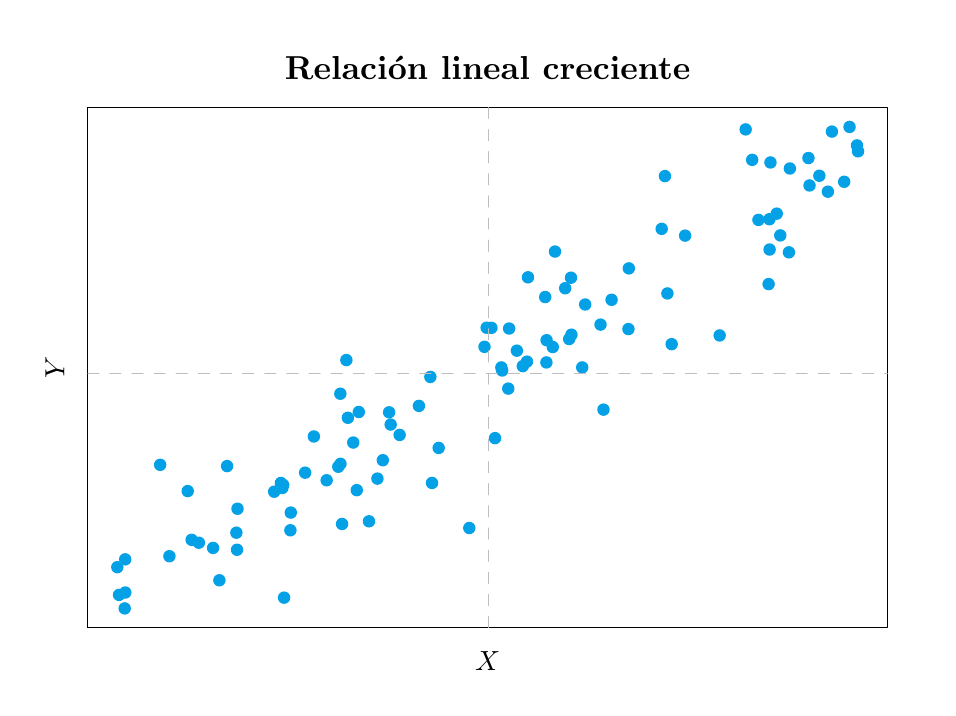
\begin{tikzpicture}[x=1pt,y=1pt]
\definecolor{fillColor}{RGB}{255,255,255}
\path[use as bounding box,fill=fillColor,fill opacity=0.00] (0,0) rectangle (325.21,238.49);
\begin{scope}
\path[clip] ( 21.68, 21.68) rectangle (310.76,209.58);
\definecolor{fillColor}{RGB}{5,161,230}

\path[fill=fillColor] (267.74,145.83) circle (  2.25);

\path[fill=fillColor] (229.09,165.79) circle (  2.25);

\path[fill=fillColor] (112.98,106.21) circle (  2.25);

\path[fill=fillColor] (264.06,169.03) circle (  2.25);

\path[fill=fillColor] (167.57,130.03) circle (  2.25);

\path[fill=fillColor] ( 92.65, 32.53) circle (  2.25);

\path[fill=fillColor] ( 47.87, 80.52) circle (  2.25);

\path[fill=fillColor] ( 33.02, 33.52) circle (  2.25);

\path[fill=fillColor] (187.00,141.15) circle (  2.25);

\path[fill=fillColor] (194.23,144.34) circle (  2.25);

\path[fill=fillColor] ( 95.08, 63.27) circle (  2.25);

\path[fill=fillColor] ( 69.27, 38.81) circle (  2.25);

\path[fill=fillColor] (250.05,127.27) circle (  2.25);

\path[fill=fillColor] (141.38,101.82) circle (  2.25);

\path[fill=fillColor] (189.74,123.09) circle (  2.25);

\path[fill=fillColor] (126.38, 75.54) circle (  2.25);

\path[fill=fillColor] ( 75.82, 64.65) circle (  2.25);

\path[fill=fillColor] (128.33, 82.19) circle (  2.25);

\path[fill=fillColor] (196.33,148.14) circle (  2.25);

\path[fill=fillColor] (100.26, 77.69) circle (  2.25);

\path[fill=fillColor] (282.52,181.47) circle (  2.25);

\path[fill=fillColor] (180.42,117.81) circle (  2.25);

\path[fill=fillColor] ( 75.65, 49.84) circle (  2.25);

\path[fill=fillColor] (113.03, 80.89) circle (  2.25);

\path[fill=fillColor] (275.42,187.60) circle (  2.25);

\path[fill=fillColor] (134.41, 91.33) circle (  2.25);

\path[fill=fillColor] (296.98,202.62) circle (  2.25);

\path[fill=fillColor] (108.04, 74.94) circle (  2.25);

\path[fill=fillColor] (268.04,169.27) circle (  2.25);

\path[fill=fillColor] ( 89.07, 70.81) circle (  2.25);

\path[fill=fillColor] ( 61.87, 52.37) circle (  2.25);

\path[fill=fillColor] ( 59.24, 53.43) circle (  2.25);

\path[fill=fillColor] (123.33, 60.12) circle (  2.25);

\path[fill=fillColor] ( 35.06, 28.64) circle (  2.25);

\path[fill=fillColor] (259.44,201.73) circle (  2.25);

\path[fill=fillColor] (146.11, 73.97) circle (  2.25);

\path[fill=fillColor] (208.07,100.47) circle (  2.25);

\path[fill=fillColor] (112.25, 79.83) circle (  2.25);

\path[fill=fillColor] (103.42, 90.77) circle (  2.25);

\path[fill=fillColor] (237.56,163.34) circle (  2.25);

\path[fill=fillColor] (195.67,125.98) circle (  2.25);

\path[fill=fillColor] (173.66,108.07) circle (  2.25);

\path[fill=fillColor] (290.61,200.94) circle (  2.25);

\path[fill=fillColor] (115.16,118.38) circle (  2.25);

\path[fill=fillColor] (119.65, 99.61) circle (  2.25);

\path[fill=fillColor] ( 57.83, 71.04) circle (  2.25);

\path[fill=fillColor] (113.60, 59.15) circle (  2.25);

\path[fill=fillColor] (217.09,129.58) circle (  2.25);

\path[fill=fillColor] (115.71, 97.52) circle (  2.25);

\path[fill=fillColor] ( 92.32, 73.26) circle (  2.25);

\path[fill=fillColor] (270.67,171.29) circle (  2.25);

\path[fill=fillColor] (268.40,189.78) circle (  2.25);

\path[fill=fillColor] (286.06,184.98) circle (  2.25);

\path[fill=fillColor] (282.13,191.38) circle (  2.25);

\path[fill=fillColor] (200.38,115.72) circle (  2.25);

\path[fill=fillColor] (275.08,157.31) circle (  2.25);

\path[fill=fillColor] (230.28,184.86) circle (  2.25);

\path[fill=fillColor] (187.51,125.55) circle (  2.25);

\path[fill=fillColor] (190.55,157.59) circle (  2.25);

\path[fill=fillColor] (289.16,179.23) circle (  2.25);

\path[fill=fillColor] (196.49,127.54) circle (  2.25);

\path[fill=fillColor] ( 67.00, 50.50) circle (  2.25);

\path[fill=fillColor] (148.51, 86.63) circle (  2.25);

\path[fill=fillColor] (171.16,115.72) circle (  2.25);

\path[fill=fillColor] (210.99,140.16) circle (  2.25);

\path[fill=fillColor] ( 32.39, 43.54) circle (  2.25);

\path[fill=fillColor] ( 94.94, 56.87) circle (  2.25);

\path[fill=fillColor] (176.77,121.78) circle (  2.25);

\path[fill=fillColor] (178.91,116.19) circle (  2.25);

\path[fill=fillColor] (159.58, 57.70) circle (  2.25);

\path[fill=fillColor] ( 72.06, 80.07) circle (  2.25);

\path[fill=fillColor] (201.45,138.46) circle (  2.25);

\path[fill=fillColor] ( 91.50, 73.96) circle (  2.25);

\path[fill=fillColor] (117.65, 88.58) circle (  2.25);

\path[fill=fillColor] (206.99,131.19) circle (  2.25);

\path[fill=fillColor] (271.95,163.43) circle (  2.25);

\path[fill=fillColor] (165.07,123.16) circle (  2.25);

\path[fill=fillColor] (268.09,158.32) circle (  2.25);

\path[fill=fillColor] (261.79,190.72) circle (  2.25);

\path[fill=fillColor] ( 92.03, 72.17) circle (  2.25);

\path[fill=fillColor] ( 75.41, 56.00) circle (  2.25);

\path[fill=fillColor] (217.23,151.51) circle (  2.25);

\path[fill=fillColor] ( 35.27, 34.38) circle (  2.25);

\path[fill=fillColor] (173.96,129.78) circle (  2.25);

\path[fill=fillColor] (231.16,142.45) circle (  2.25);

\path[fill=fillColor] (145.51,112.29) circle (  2.25);

\path[fill=fillColor] (299.67,195.94) circle (  2.25);

\path[fill=fillColor] (168.88, 90.17) circle (  2.25);

\path[fill=fillColor] (165.85,130.07) circle (  2.25);

\path[fill=fillColor] (232.70,124.13) circle (  2.25);

\path[fill=fillColor] (295.04,182.80) circle (  2.25);

\path[fill=fillColor] (187.44,117.52) circle (  2.25);

\path[fill=fillColor] (171.45,114.61) circle (  2.25);

\path[fill=fillColor] (130.61, 99.50) circle (  2.25);

\path[fill=fillColor] (118.92, 71.37) circle (  2.25);

\path[fill=fillColor] (300.05,193.81) circle (  2.25);

\path[fill=fillColor] (180.78,148.28) circle (  2.25);

\path[fill=fillColor] ( 51.22, 47.50) circle (  2.25);

\path[fill=fillColor] (131.17, 95.07) circle (  2.25);

\path[fill=fillColor] ( 35.24, 46.37) circle (  2.25);
\end{scope}
\begin{scope}
\path[clip] (  0.00,  0.00) rectangle (325.21,238.49);
\definecolor{drawColor}{RGB}{0,0,0}

\node[text=drawColor,anchor=base,inner sep=0pt, outer sep=0pt, scale=  1.20] at (166.22,219.84) {\bfseries Relación lineal creciente};

\node[text=drawColor,anchor=base,inner sep=0pt, outer sep=0pt, scale=  1.00] at (166.22,  6.08) {$X$};

\node[text=drawColor,rotate= 90.00,anchor=base,inner sep=0pt, outer sep=0pt, scale=  1.00] at ( 13.28,115.63) {$Y$};
\end{scope}
\begin{scope}
\path[clip] (  0.00,  0.00) rectangle (325.21,238.49);
\definecolor{drawColor}{RGB}{0,0,0}

\path[draw=drawColor,line width= 0.4pt,line join=round,line cap=round] ( 21.68, 21.68) --
	(310.76, 21.68) --
	(310.76,209.58) --
	( 21.68,209.58) --
	( 21.68, 21.68);
\end{scope}
\begin{scope}
\path[clip] ( 21.68, 21.68) rectangle (310.76,209.58);
\definecolor{drawColor}{RGB}{190,190,190}

\path[draw=drawColor,line width= 0.4pt,dash pattern=on 4pt off 4pt ,line join=round,line cap=round] ( 21.68,113.44) -- (310.76,113.44);

\path[draw=drawColor,line width= 0.4pt,dash pattern=on 4pt off 4pt ,line join=round,line cap=round] (166.43, 21.68) -- (166.43,209.58);
\end{scope}
\end{tikzpicture}
}}
\mode<presentation>{\resizebox{0.9\textwidth}{!}{% Created by tikzDevice version 0.10.1 on 2016-02-27 12:54:11
% !TEX encoding = UTF-8 Unicode
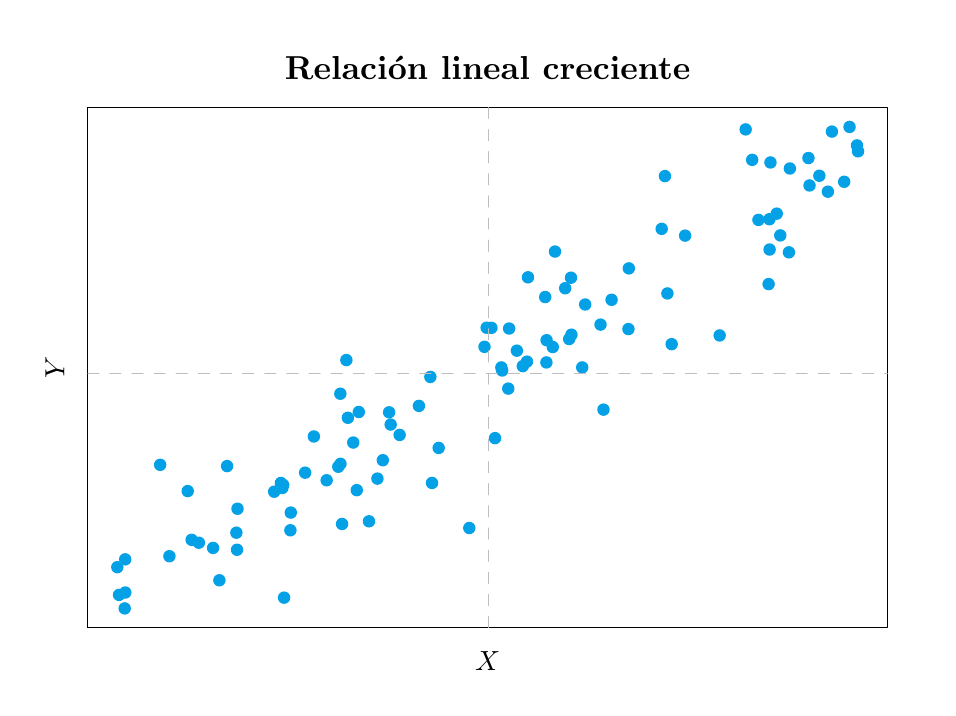
\begin{tikzpicture}[x=1pt,y=1pt]
\definecolor{fillColor}{RGB}{255,255,255}
\path[use as bounding box,fill=fillColor,fill opacity=0.00] (0,0) rectangle (325.21,238.49);
\begin{scope}
\path[clip] ( 21.68, 21.68) rectangle (310.76,209.58);
\definecolor{fillColor}{RGB}{5,161,230}

\path[fill=fillColor] (267.74,145.83) circle (  2.25);

\path[fill=fillColor] (229.09,165.79) circle (  2.25);

\path[fill=fillColor] (112.98,106.21) circle (  2.25);

\path[fill=fillColor] (264.06,169.03) circle (  2.25);

\path[fill=fillColor] (167.57,130.03) circle (  2.25);

\path[fill=fillColor] ( 92.65, 32.53) circle (  2.25);

\path[fill=fillColor] ( 47.87, 80.52) circle (  2.25);

\path[fill=fillColor] ( 33.02, 33.52) circle (  2.25);

\path[fill=fillColor] (187.00,141.15) circle (  2.25);

\path[fill=fillColor] (194.23,144.34) circle (  2.25);

\path[fill=fillColor] ( 95.08, 63.27) circle (  2.25);

\path[fill=fillColor] ( 69.27, 38.81) circle (  2.25);

\path[fill=fillColor] (250.05,127.27) circle (  2.25);

\path[fill=fillColor] (141.38,101.82) circle (  2.25);

\path[fill=fillColor] (189.74,123.09) circle (  2.25);

\path[fill=fillColor] (126.38, 75.54) circle (  2.25);

\path[fill=fillColor] ( 75.82, 64.65) circle (  2.25);

\path[fill=fillColor] (128.33, 82.19) circle (  2.25);

\path[fill=fillColor] (196.33,148.14) circle (  2.25);

\path[fill=fillColor] (100.26, 77.69) circle (  2.25);

\path[fill=fillColor] (282.52,181.47) circle (  2.25);

\path[fill=fillColor] (180.42,117.81) circle (  2.25);

\path[fill=fillColor] ( 75.65, 49.84) circle (  2.25);

\path[fill=fillColor] (113.03, 80.89) circle (  2.25);

\path[fill=fillColor] (275.42,187.60) circle (  2.25);

\path[fill=fillColor] (134.41, 91.33) circle (  2.25);

\path[fill=fillColor] (296.98,202.62) circle (  2.25);

\path[fill=fillColor] (108.04, 74.94) circle (  2.25);

\path[fill=fillColor] (268.04,169.27) circle (  2.25);

\path[fill=fillColor] ( 89.07, 70.81) circle (  2.25);

\path[fill=fillColor] ( 61.87, 52.37) circle (  2.25);

\path[fill=fillColor] ( 59.24, 53.43) circle (  2.25);

\path[fill=fillColor] (123.33, 60.12) circle (  2.25);

\path[fill=fillColor] ( 35.06, 28.64) circle (  2.25);

\path[fill=fillColor] (259.44,201.73) circle (  2.25);

\path[fill=fillColor] (146.11, 73.97) circle (  2.25);

\path[fill=fillColor] (208.07,100.47) circle (  2.25);

\path[fill=fillColor] (112.25, 79.83) circle (  2.25);

\path[fill=fillColor] (103.42, 90.77) circle (  2.25);

\path[fill=fillColor] (237.56,163.34) circle (  2.25);

\path[fill=fillColor] (195.67,125.98) circle (  2.25);

\path[fill=fillColor] (173.66,108.07) circle (  2.25);

\path[fill=fillColor] (290.61,200.94) circle (  2.25);

\path[fill=fillColor] (115.16,118.38) circle (  2.25);

\path[fill=fillColor] (119.65, 99.61) circle (  2.25);

\path[fill=fillColor] ( 57.83, 71.04) circle (  2.25);

\path[fill=fillColor] (113.60, 59.15) circle (  2.25);

\path[fill=fillColor] (217.09,129.58) circle (  2.25);

\path[fill=fillColor] (115.71, 97.52) circle (  2.25);

\path[fill=fillColor] ( 92.32, 73.26) circle (  2.25);

\path[fill=fillColor] (270.67,171.29) circle (  2.25);

\path[fill=fillColor] (268.40,189.78) circle (  2.25);

\path[fill=fillColor] (286.06,184.98) circle (  2.25);

\path[fill=fillColor] (282.13,191.38) circle (  2.25);

\path[fill=fillColor] (200.38,115.72) circle (  2.25);

\path[fill=fillColor] (275.08,157.31) circle (  2.25);

\path[fill=fillColor] (230.28,184.86) circle (  2.25);

\path[fill=fillColor] (187.51,125.55) circle (  2.25);

\path[fill=fillColor] (190.55,157.59) circle (  2.25);

\path[fill=fillColor] (289.16,179.23) circle (  2.25);

\path[fill=fillColor] (196.49,127.54) circle (  2.25);

\path[fill=fillColor] ( 67.00, 50.50) circle (  2.25);

\path[fill=fillColor] (148.51, 86.63) circle (  2.25);

\path[fill=fillColor] (171.16,115.72) circle (  2.25);

\path[fill=fillColor] (210.99,140.16) circle (  2.25);

\path[fill=fillColor] ( 32.39, 43.54) circle (  2.25);

\path[fill=fillColor] ( 94.94, 56.87) circle (  2.25);

\path[fill=fillColor] (176.77,121.78) circle (  2.25);

\path[fill=fillColor] (178.91,116.19) circle (  2.25);

\path[fill=fillColor] (159.58, 57.70) circle (  2.25);

\path[fill=fillColor] ( 72.06, 80.07) circle (  2.25);

\path[fill=fillColor] (201.45,138.46) circle (  2.25);

\path[fill=fillColor] ( 91.50, 73.96) circle (  2.25);

\path[fill=fillColor] (117.65, 88.58) circle (  2.25);

\path[fill=fillColor] (206.99,131.19) circle (  2.25);

\path[fill=fillColor] (271.95,163.43) circle (  2.25);

\path[fill=fillColor] (165.07,123.16) circle (  2.25);

\path[fill=fillColor] (268.09,158.32) circle (  2.25);

\path[fill=fillColor] (261.79,190.72) circle (  2.25);

\path[fill=fillColor] ( 92.03, 72.17) circle (  2.25);

\path[fill=fillColor] ( 75.41, 56.00) circle (  2.25);

\path[fill=fillColor] (217.23,151.51) circle (  2.25);

\path[fill=fillColor] ( 35.27, 34.38) circle (  2.25);

\path[fill=fillColor] (173.96,129.78) circle (  2.25);

\path[fill=fillColor] (231.16,142.45) circle (  2.25);

\path[fill=fillColor] (145.51,112.29) circle (  2.25);

\path[fill=fillColor] (299.67,195.94) circle (  2.25);

\path[fill=fillColor] (168.88, 90.17) circle (  2.25);

\path[fill=fillColor] (165.85,130.07) circle (  2.25);

\path[fill=fillColor] (232.70,124.13) circle (  2.25);

\path[fill=fillColor] (295.04,182.80) circle (  2.25);

\path[fill=fillColor] (187.44,117.52) circle (  2.25);

\path[fill=fillColor] (171.45,114.61) circle (  2.25);

\path[fill=fillColor] (130.61, 99.50) circle (  2.25);

\path[fill=fillColor] (118.92, 71.37) circle (  2.25);

\path[fill=fillColor] (300.05,193.81) circle (  2.25);

\path[fill=fillColor] (180.78,148.28) circle (  2.25);

\path[fill=fillColor] ( 51.22, 47.50) circle (  2.25);

\path[fill=fillColor] (131.17, 95.07) circle (  2.25);

\path[fill=fillColor] ( 35.24, 46.37) circle (  2.25);
\end{scope}
\begin{scope}
\path[clip] (  0.00,  0.00) rectangle (325.21,238.49);
\definecolor{drawColor}{RGB}{0,0,0}

\node[text=drawColor,anchor=base,inner sep=0pt, outer sep=0pt, scale=  1.20] at (166.22,219.84) {\bfseries Relación lineal creciente};

\node[text=drawColor,anchor=base,inner sep=0pt, outer sep=0pt, scale=  1.00] at (166.22,  6.08) {$X$};

\node[text=drawColor,rotate= 90.00,anchor=base,inner sep=0pt, outer sep=0pt, scale=  1.00] at ( 13.28,115.63) {$Y$};
\end{scope}
\begin{scope}
\path[clip] (  0.00,  0.00) rectangle (325.21,238.49);
\definecolor{drawColor}{RGB}{0,0,0}

\path[draw=drawColor,line width= 0.4pt,line join=round,line cap=round] ( 21.68, 21.68) --
	(310.76, 21.68) --
	(310.76,209.58) --
	( 21.68,209.58) --
	( 21.68, 21.68);
\end{scope}
\begin{scope}
\path[clip] ( 21.68, 21.68) rectangle (310.76,209.58);
\definecolor{drawColor}{RGB}{190,190,190}

\path[draw=drawColor,line width= 0.4pt,dash pattern=on 4pt off 4pt ,line join=round,line cap=round] ( 21.68,113.44) -- (310.76,113.44);

\path[draw=drawColor,line width= 0.4pt,dash pattern=on 4pt off 4pt ,line join=round,line cap=round] (166.43, 21.68) -- (166.43,209.58);
\end{scope}
\end{tikzpicture}
}}

\[
\sum(x_i-\bar x)(y_j-\bar y) = +
\]
\end{column}
\begin{column}{0.5\textwidth}
Si la relación entre las variables es \emph{lineal y decreciente}, entonces la mayor parte de los puntos estarán en los cuadrantes 2 y 4 y la suma de los productos de desviaciones será negativa.

\centering
\tikzsetnextfilename{regresion/diagrama_dispersion_lineal_decreciente}
\mode<article>{\resizebox{0.6\textwidth}{!}{% Created by tikzDevice version 0.10.1 on 2016-02-27 12:54:12
% !TEX encoding = UTF-8 Unicode
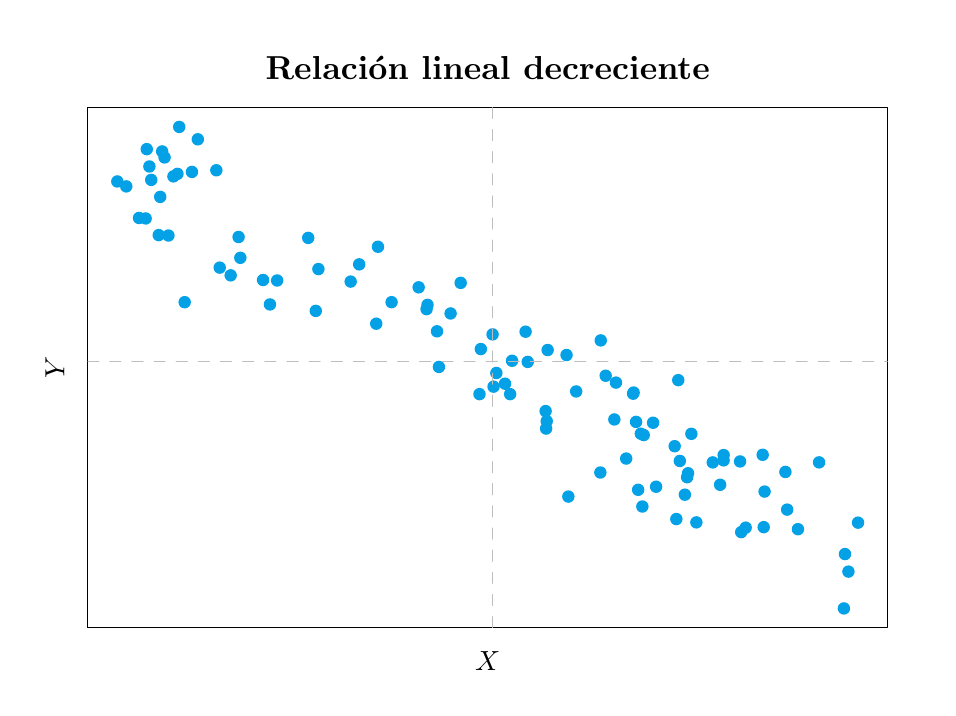
\begin{tikzpicture}[x=1pt,y=1pt]
\definecolor{fillColor}{RGB}{255,255,255}
\path[use as bounding box,fill=fillColor,fill opacity=0.00] (0,0) rectangle (325.21,238.49);
\begin{scope}
\path[clip] ( 21.68, 21.68) rectangle (310.76,209.58);
\definecolor{fillColor}{RGB}{5,161,230}

\path[fill=fillColor] (257.84, 56.21) circle (  2.25);

\path[fill=fillColor] (247.55, 81.40) circle (  2.25);

\path[fill=fillColor] (172.49,109.84) circle (  2.25);

\path[fill=fillColor] (180.69,117.72) circle (  2.25);

\path[fill=fillColor] (207.08,125.48) circle (  2.25);

\path[fill=fillColor] (187.55, 96.32) circle (  2.25);

\path[fill=fillColor] (156.46,146.27) circle (  2.25);

\path[fill=fillColor] ( 35.63,181.13) circle (  2.25);

\path[fill=fillColor] (222.11, 65.46) circle (  2.25);

\path[fill=fillColor] ( 73.35,148.99) circle (  2.25);

\path[fill=fillColor] (167.99,127.66) circle (  2.25);

\path[fill=fillColor] ( 47.35,163.54) circle (  2.25);

\path[fill=fillColor] (233.79, 87.25) circle (  2.25);

\path[fill=fillColor] (194.72,120.20) circle (  2.25);

\path[fill=fillColor] (104.10,136.14) circle (  2.25);

\path[fill=fillColor] ( 48.59,193.77) circle (  2.25);

\path[fill=fillColor] (273.80, 77.96) circle (  2.25);

\path[fill=fillColor] ( 42.63,169.55) circle (  2.25);

\path[fill=fillColor] (219.84, 96.04) circle (  2.25);

\path[fill=fillColor] (195.37, 69.05) circle (  2.25);

\path[fill=fillColor] (152.82,135.22) circle (  2.25);

\path[fill=fillColor] (169.36,113.71) circle (  2.25);

\path[fill=fillColor] (265.96, 58.00) circle (  2.25);

\path[fill=fillColor] (296.58, 41.94) circle (  2.25);

\path[fill=fillColor] (147.92,128.77) circle (  2.25);

\path[fill=fillColor] ( 43.03,194.59) circle (  2.25);

\path[fill=fillColor] (105.05,151.26) circle (  2.25);

\path[fill=fillColor] ( 59.35,186.37) circle (  2.25);

\path[fill=fillColor] ( 50.87,163.38) circle (  2.25);

\path[fill=fillColor] ( 43.98,188.33) circle (  2.25);

\path[fill=fillColor] (218.95,106.65) circle (  2.25);

\path[fill=fillColor] (250.22, 73.32) circle (  2.25);

\path[fill=fillColor] (119.79,152.96) circle (  2.25);

\path[fill=fillColor] (116.71,146.74) circle (  2.25);

\path[fill=fillColor] (251.49, 84.05) circle (  2.25);

\path[fill=fillColor] ( 44.65,183.48) circle (  2.25);

\path[fill=fillColor] ( 61.48,198.15) circle (  2.25);

\path[fill=fillColor] (222.61, 91.28) circle (  2.25);

\path[fill=fillColor] (266.28, 70.86) circle (  2.25);

\path[fill=fillColor] (126.58,159.32) circle (  2.25);

\path[fill=fillColor] ( 54.76,202.62) circle (  2.25);

\path[fill=fillColor] (251.47, 82.13) circle (  2.25);

\path[fill=fillColor] (144.14,136.78) circle (  2.25);

\path[fill=fillColor] (144.48,138.31) circle (  2.25);

\path[fill=fillColor] (216.27, 82.79) circle (  2.25);

\path[fill=fillColor] ( 47.89,177.34) circle (  2.25);

\path[fill=fillColor] (175.03,118.13) circle (  2.25);

\path[fill=fillColor] (274.44, 64.34) circle (  2.25);

\path[fill=fillColor] (163.26,106.07) circle (  2.25);

\path[fill=fillColor] (148.60,115.90) circle (  2.25);

\path[fill=fillColor] ( 90.15,147.14) circle (  2.25);

\path[fill=fillColor] ( 49.47,191.59) circle (  2.25);

\path[fill=fillColor] (218.77,106.23) circle (  2.25);

\path[fill=fillColor] (300.05, 59.63) circle (  2.25);

\path[fill=fillColor] (101.37,162.52) circle (  2.25);

\path[fill=fillColor] ( 76.21,162.85) circle (  2.25);

\path[fill=fillColor] (241.63, 59.72) circle (  2.25);

\path[fill=fillColor] (259.45, 57.82) circle (  2.25);

\path[fill=fillColor] (235.65, 81.92) circle (  2.25);

\path[fill=fillColor] (221.56, 91.77) circle (  2.25);

\path[fill=fillColor] (187.34, 93.63) circle (  2.25);

\path[fill=fillColor] ( 76.85,155.33) circle (  2.25);

\path[fill=fillColor] (285.97, 81.41) circle (  2.25);

\path[fill=fillColor] (212.58,110.24) circle (  2.25);

\path[fill=fillColor] (206.94, 77.75) circle (  2.25);

\path[fill=fillColor] ( 40.24,169.73) circle (  2.25);

\path[fill=fillColor] ( 87.55,138.48) circle (  2.25);

\path[fill=fillColor] ( 32.39,182.92) circle (  2.25);

\path[fill=fillColor] ( 52.67,184.75) circle (  2.25);

\path[fill=fillColor] (278.34, 57.27) circle (  2.25);

\path[fill=fillColor] (257.42, 81.74) circle (  2.25);

\path[fill=fillColor] ( 69.39,151.78) circle (  2.25);

\path[fill=fillColor] (187.16, 99.94) circle (  2.25);

\path[fill=fillColor] (198.20,107.04) circle (  2.25);

\path[fill=fillColor] (220.59, 71.50) circle (  2.25);

\path[fill=fillColor] (238.28, 76.05) circle (  2.25);

\path[fill=fillColor] (131.50,139.30) circle (  2.25);

\path[fill=fillColor] (227.08, 72.61) circle (  2.25);

\path[fill=fillColor] (141.28,144.66) circle (  2.25);

\path[fill=fillColor] (163.75,122.35) circle (  2.25);

\path[fill=fillColor] ( 68.17,186.96) circle (  2.25);

\path[fill=fillColor] (265.59, 84.15) circle (  2.25);

\path[fill=fillColor] ( 85.06,147.31) circle (  2.25);

\path[fill=fillColor] (168.35,108.77) circle (  2.25);

\path[fill=fillColor] (211.99, 96.92) circle (  2.25);

\path[fill=fillColor] (174.34,106.07) circle (  2.25);

\path[fill=fillColor] ( 56.73,139.29) circle (  2.25);

\path[fill=fillColor] (294.94, 28.64) circle (  2.25);

\path[fill=fillColor] (225.99, 95.73) circle (  2.25);

\path[fill=fillColor] (239.82, 91.72) circle (  2.25);

\path[fill=fillColor] (237.48, 69.74) circle (  2.25);

\path[fill=fillColor] (187.89,122.01) circle (  2.25);

\path[fill=fillColor] (295.34, 48.28) circle (  2.25);

\path[fill=fillColor] (208.86,112.72) circle (  2.25);

\path[fill=fillColor] ( 54.11,185.66) circle (  2.25);

\path[fill=fillColor] (235.09,111.12) circle (  2.25);

\path[fill=fillColor] (234.40, 60.93) circle (  2.25);

\path[fill=fillColor] (179.92,128.63) circle (  2.25);

\path[fill=fillColor] (125.95,131.52) circle (  2.25);

\path[fill=fillColor] (238.62, 77.48) circle (  2.25);
\end{scope}
\begin{scope}
\path[clip] (  0.00,  0.00) rectangle (325.21,238.49);
\definecolor{drawColor}{RGB}{0,0,0}

\node[text=drawColor,anchor=base,inner sep=0pt, outer sep=0pt, scale=  1.20] at (166.22,219.84) {\bfseries Relación lineal decreciente};

\node[text=drawColor,anchor=base,inner sep=0pt, outer sep=0pt, scale=  1.00] at (166.22,  6.08) {$X$};

\node[text=drawColor,rotate= 90.00,anchor=base,inner sep=0pt, outer sep=0pt, scale=  1.00] at ( 13.28,115.63) {$Y$};
\end{scope}
\begin{scope}
\path[clip] (  0.00,  0.00) rectangle (325.21,238.49);
\definecolor{drawColor}{RGB}{0,0,0}

\path[draw=drawColor,line width= 0.4pt,line join=round,line cap=round] ( 21.68, 21.68) --
	(310.76, 21.68) --
	(310.76,209.58) --
	( 21.68,209.58) --
	( 21.68, 21.68);
\end{scope}
\begin{scope}
\path[clip] ( 21.68, 21.68) rectangle (310.76,209.58);
\definecolor{drawColor}{RGB}{190,190,190}

\path[draw=drawColor,line width= 0.4pt,dash pattern=on 4pt off 4pt ,line join=round,line cap=round] ( 21.68,117.96) -- (310.76,117.96);

\path[draw=drawColor,line width= 0.4pt,dash pattern=on 4pt off 4pt ,line join=round,line cap=round] (167.81, 21.68) -- (167.81,209.58);
\end{scope}
\end{tikzpicture}
}}
\mode<presentation>{\resizebox{0.9\textwidth}{!}{% Created by tikzDevice version 0.10.1 on 2016-02-27 12:54:12
% !TEX encoding = UTF-8 Unicode
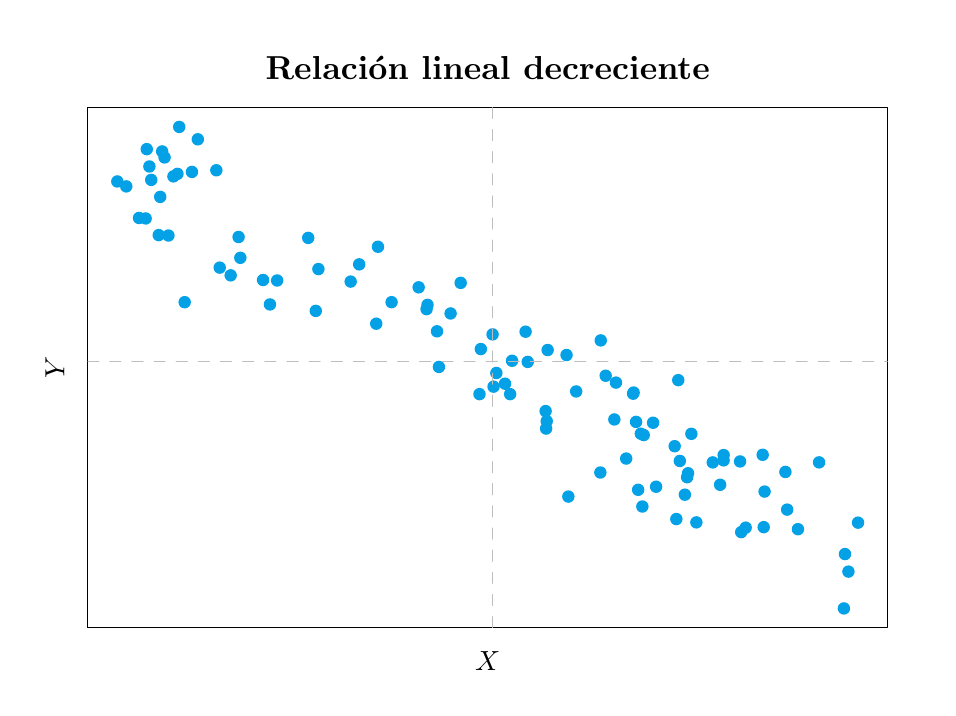
\begin{tikzpicture}[x=1pt,y=1pt]
\definecolor{fillColor}{RGB}{255,255,255}
\path[use as bounding box,fill=fillColor,fill opacity=0.00] (0,0) rectangle (325.21,238.49);
\begin{scope}
\path[clip] ( 21.68, 21.68) rectangle (310.76,209.58);
\definecolor{fillColor}{RGB}{5,161,230}

\path[fill=fillColor] (257.84, 56.21) circle (  2.25);

\path[fill=fillColor] (247.55, 81.40) circle (  2.25);

\path[fill=fillColor] (172.49,109.84) circle (  2.25);

\path[fill=fillColor] (180.69,117.72) circle (  2.25);

\path[fill=fillColor] (207.08,125.48) circle (  2.25);

\path[fill=fillColor] (187.55, 96.32) circle (  2.25);

\path[fill=fillColor] (156.46,146.27) circle (  2.25);

\path[fill=fillColor] ( 35.63,181.13) circle (  2.25);

\path[fill=fillColor] (222.11, 65.46) circle (  2.25);

\path[fill=fillColor] ( 73.35,148.99) circle (  2.25);

\path[fill=fillColor] (167.99,127.66) circle (  2.25);

\path[fill=fillColor] ( 47.35,163.54) circle (  2.25);

\path[fill=fillColor] (233.79, 87.25) circle (  2.25);

\path[fill=fillColor] (194.72,120.20) circle (  2.25);

\path[fill=fillColor] (104.10,136.14) circle (  2.25);

\path[fill=fillColor] ( 48.59,193.77) circle (  2.25);

\path[fill=fillColor] (273.80, 77.96) circle (  2.25);

\path[fill=fillColor] ( 42.63,169.55) circle (  2.25);

\path[fill=fillColor] (219.84, 96.04) circle (  2.25);

\path[fill=fillColor] (195.37, 69.05) circle (  2.25);

\path[fill=fillColor] (152.82,135.22) circle (  2.25);

\path[fill=fillColor] (169.36,113.71) circle (  2.25);

\path[fill=fillColor] (265.96, 58.00) circle (  2.25);

\path[fill=fillColor] (296.58, 41.94) circle (  2.25);

\path[fill=fillColor] (147.92,128.77) circle (  2.25);

\path[fill=fillColor] ( 43.03,194.59) circle (  2.25);

\path[fill=fillColor] (105.05,151.26) circle (  2.25);

\path[fill=fillColor] ( 59.35,186.37) circle (  2.25);

\path[fill=fillColor] ( 50.87,163.38) circle (  2.25);

\path[fill=fillColor] ( 43.98,188.33) circle (  2.25);

\path[fill=fillColor] (218.95,106.65) circle (  2.25);

\path[fill=fillColor] (250.22, 73.32) circle (  2.25);

\path[fill=fillColor] (119.79,152.96) circle (  2.25);

\path[fill=fillColor] (116.71,146.74) circle (  2.25);

\path[fill=fillColor] (251.49, 84.05) circle (  2.25);

\path[fill=fillColor] ( 44.65,183.48) circle (  2.25);

\path[fill=fillColor] ( 61.48,198.15) circle (  2.25);

\path[fill=fillColor] (222.61, 91.28) circle (  2.25);

\path[fill=fillColor] (266.28, 70.86) circle (  2.25);

\path[fill=fillColor] (126.58,159.32) circle (  2.25);

\path[fill=fillColor] ( 54.76,202.62) circle (  2.25);

\path[fill=fillColor] (251.47, 82.13) circle (  2.25);

\path[fill=fillColor] (144.14,136.78) circle (  2.25);

\path[fill=fillColor] (144.48,138.31) circle (  2.25);

\path[fill=fillColor] (216.27, 82.79) circle (  2.25);

\path[fill=fillColor] ( 47.89,177.34) circle (  2.25);

\path[fill=fillColor] (175.03,118.13) circle (  2.25);

\path[fill=fillColor] (274.44, 64.34) circle (  2.25);

\path[fill=fillColor] (163.26,106.07) circle (  2.25);

\path[fill=fillColor] (148.60,115.90) circle (  2.25);

\path[fill=fillColor] ( 90.15,147.14) circle (  2.25);

\path[fill=fillColor] ( 49.47,191.59) circle (  2.25);

\path[fill=fillColor] (218.77,106.23) circle (  2.25);

\path[fill=fillColor] (300.05, 59.63) circle (  2.25);

\path[fill=fillColor] (101.37,162.52) circle (  2.25);

\path[fill=fillColor] ( 76.21,162.85) circle (  2.25);

\path[fill=fillColor] (241.63, 59.72) circle (  2.25);

\path[fill=fillColor] (259.45, 57.82) circle (  2.25);

\path[fill=fillColor] (235.65, 81.92) circle (  2.25);

\path[fill=fillColor] (221.56, 91.77) circle (  2.25);

\path[fill=fillColor] (187.34, 93.63) circle (  2.25);

\path[fill=fillColor] ( 76.85,155.33) circle (  2.25);

\path[fill=fillColor] (285.97, 81.41) circle (  2.25);

\path[fill=fillColor] (212.58,110.24) circle (  2.25);

\path[fill=fillColor] (206.94, 77.75) circle (  2.25);

\path[fill=fillColor] ( 40.24,169.73) circle (  2.25);

\path[fill=fillColor] ( 87.55,138.48) circle (  2.25);

\path[fill=fillColor] ( 32.39,182.92) circle (  2.25);

\path[fill=fillColor] ( 52.67,184.75) circle (  2.25);

\path[fill=fillColor] (278.34, 57.27) circle (  2.25);

\path[fill=fillColor] (257.42, 81.74) circle (  2.25);

\path[fill=fillColor] ( 69.39,151.78) circle (  2.25);

\path[fill=fillColor] (187.16, 99.94) circle (  2.25);

\path[fill=fillColor] (198.20,107.04) circle (  2.25);

\path[fill=fillColor] (220.59, 71.50) circle (  2.25);

\path[fill=fillColor] (238.28, 76.05) circle (  2.25);

\path[fill=fillColor] (131.50,139.30) circle (  2.25);

\path[fill=fillColor] (227.08, 72.61) circle (  2.25);

\path[fill=fillColor] (141.28,144.66) circle (  2.25);

\path[fill=fillColor] (163.75,122.35) circle (  2.25);

\path[fill=fillColor] ( 68.17,186.96) circle (  2.25);

\path[fill=fillColor] (265.59, 84.15) circle (  2.25);

\path[fill=fillColor] ( 85.06,147.31) circle (  2.25);

\path[fill=fillColor] (168.35,108.77) circle (  2.25);

\path[fill=fillColor] (211.99, 96.92) circle (  2.25);

\path[fill=fillColor] (174.34,106.07) circle (  2.25);

\path[fill=fillColor] ( 56.73,139.29) circle (  2.25);

\path[fill=fillColor] (294.94, 28.64) circle (  2.25);

\path[fill=fillColor] (225.99, 95.73) circle (  2.25);

\path[fill=fillColor] (239.82, 91.72) circle (  2.25);

\path[fill=fillColor] (237.48, 69.74) circle (  2.25);

\path[fill=fillColor] (187.89,122.01) circle (  2.25);

\path[fill=fillColor] (295.34, 48.28) circle (  2.25);

\path[fill=fillColor] (208.86,112.72) circle (  2.25);

\path[fill=fillColor] ( 54.11,185.66) circle (  2.25);

\path[fill=fillColor] (235.09,111.12) circle (  2.25);

\path[fill=fillColor] (234.40, 60.93) circle (  2.25);

\path[fill=fillColor] (179.92,128.63) circle (  2.25);

\path[fill=fillColor] (125.95,131.52) circle (  2.25);

\path[fill=fillColor] (238.62, 77.48) circle (  2.25);
\end{scope}
\begin{scope}
\path[clip] (  0.00,  0.00) rectangle (325.21,238.49);
\definecolor{drawColor}{RGB}{0,0,0}

\node[text=drawColor,anchor=base,inner sep=0pt, outer sep=0pt, scale=  1.20] at (166.22,219.84) {\bfseries Relación lineal decreciente};

\node[text=drawColor,anchor=base,inner sep=0pt, outer sep=0pt, scale=  1.00] at (166.22,  6.08) {$X$};

\node[text=drawColor,rotate= 90.00,anchor=base,inner sep=0pt, outer sep=0pt, scale=  1.00] at ( 13.28,115.63) {$Y$};
\end{scope}
\begin{scope}
\path[clip] (  0.00,  0.00) rectangle (325.21,238.49);
\definecolor{drawColor}{RGB}{0,0,0}

\path[draw=drawColor,line width= 0.4pt,line join=round,line cap=round] ( 21.68, 21.68) --
	(310.76, 21.68) --
	(310.76,209.58) --
	( 21.68,209.58) --
	( 21.68, 21.68);
\end{scope}
\begin{scope}
\path[clip] ( 21.68, 21.68) rectangle (310.76,209.58);
\definecolor{drawColor}{RGB}{190,190,190}

\path[draw=drawColor,line width= 0.4pt,dash pattern=on 4pt off 4pt ,line join=round,line cap=round] ( 21.68,117.96) -- (310.76,117.96);

\path[draw=drawColor,line width= 0.4pt,dash pattern=on 4pt off 4pt ,line join=round,line cap=round] (167.81, 21.68) -- (167.81,209.58);
\end{scope}
\end{tikzpicture}
}}

\[
\sum(x_i-\bar x)(y_j-\bar y) = -
\]
\end{column}
\end{columns}

\note{Si la relación entre las variables es lineal y creciente, como refleja el primer diagrama de dispersión, entonces la mayor parte de
los puntos estarán en los cuadrantes 1 y 3, y por tanto habrá muchos más puntos cuyo producto de desviaciones sea positivo, que puntos
cuyo producto de desviaciones sea negativo, de manera que la suma de los productos de desviaciones de todos los puntos será positiva.

Por contra, cuando la relación entre las variables sea lineal y decreciente, como ocurre en el segundo diagrama, entonces la la mayor parte de
los puntos estarán en los cuadrantes 2 y 4, y por tanto habrá muchos más puntos cuyo producto de desviaciones sea negativo, que puntos
cuyo producto de desviaciones sea positivo, de manera que la suma de los productos de desviaciones de todos los puntos será negativa.
}
\end{frame}


%---------------------------------------------------------------------slide----
\begin{frame}
\frametitle{Covarianza}
Usando el producto de las desviaciones respecto de las medias surge el siguiente estadístico.

\begin{definicion}[Covarianza muestral]
La \emph{covarianza muestral} de una variable aleatoria bidimensional $(X,Y)$ se define como el promedio de los
productos de las respectivas desviaciones respecto de las medias de $X$ e $Y$.
\[
s_{xy}=\frac{\sum (x_i-\bar x)(y_j-\bar y)n_{ij}}{n}
\]
\end{definicion}
También puede calcularse de manera más sencilla mediante la fórmula
\[
s_{xy}=\frac{\sum x_iy_jn_{ij}}{n}-\bar x\bar y.
\]
La covarianza sirve para estudiar la relación lineal entre dos variables:
\begin{itemize}
\item Si $s_{xy}>0$ existe una relación lineal creciente entre las variables.
\item Si $s_{xy}<0$ existe una relación lineal decreciente entre las variables.
\item Si $s_{xy}=0$ no existe relación lineal entre las variables. 
\end{itemize} 

\note{Del razonamiento anterior surge un estadístico conocido como covarianza para estudiar la relación lineal entre variables.

La covarianza, que se representa $s_{xy}$ se define como la suma de los productos de las desviaciones a las respectivas medias,
multiplicadas por la frecuencia absoluta relativa de cada par y dividido por el tamaño de la muestra.

Si se desarrolla el producto de las desviaciones y se simplifica, se llega a una fórmula equivalente para el cálculo de la covarianza que
consiste en sumar los productos del valor de $X$ por el valor de $Y$ en cada individuo, por la frecuencia absoluta del par, dividido por el
tamaño de la muestra y restarle al cociente el producto de las medias de $X$ e $Y$. Esta fórmula es un poco más fácil de aplicar y por
tanto será la que utilizaremos a lo largo del tema.

A la hora de interpretar la covarianza como medida de relación lineal, lo más importante es su signo, ya que como vimos antes, si existe
relación lineal creciente entre las variables, la suma de los productos de las desviaciones será positiva y también lo será la
covarianza; si la relación es lineal decreciente, la suma de los productos de las desviaciones será negativa y también lo será la
covarianza; mientras que si no hay relación lineal, los puntos se distribuirán más o menos por igual en los cuatro cuadrantes y se
compensarán los productos de desviaciones positivos con los negativos, con lo que la covarianza valdrá aproximadamente 0.

Hay que tener en cuenta que la covarianza tiene unidades, que son el producto de las unidades de $X$ e $Y$, lo cual dificulta su
interpretación a la hora de valorar el grado de dependencia lineal entre las variables, aunque, como veremos más adelante, a partir de ella
es posible obtener una medida adimensional que si permitirá estudiar el grado de dependencia lineal.}
\end{frame}


%---------------------------------------------------------------------slide----
\begin{frame}
\frametitle{Cálculo de la covarianza}
\framesubtitle{Ejemplo con estaturas y pesos}
En el ejemplo de las estaturas y pesos, teniendo en cuenta que 
\[
\begin{array}{|c||c|c|c|c|c|c|c|}
\hline
  X/Y & [50,60) & [60,70) & [70,80) & [80,90) & [90,100) & [100,110) & n_x\\
  \hline\hline
  (150,160] & 2 & 0 & 0 & 0 & 0 & 0 & 2\\
  \hline
  (160,170] & 4 & 4 & 0 & 0 & 0 & 0 & 8\\
  \hline
  (170,180] & 1 & 6 & 3 & 1 & 0 & 0 & 11 \\
  \hline
  (180,190] & 0 & 1 & 4 & 1 & 1 & 0 & 7 \\
  \hline
  (190,200] & 0 & 0 & 0 & 0 & 1 & 1 & 2\\
  \hline
  n_y & 7 & 11 & 7 & 2 & 2 & 1 & 30\\
  \hline
\end{array}
\]
\[
\bar x = 174.67 \mbox{ cm} \qquad \bar y = 69.67 \mbox{ Kg} 
\]
la covarianza vale
\begin{align*}
s_{xy} &=\frac{\sum x_iy_jn_{ij}}{n}-\bar x\bar y =  \frac{155\cdot 55\cdot 2 + 165\cdot 55\cdot 4 + \cdots + 195\cdot 105\cdot 1}{30}-174.67\cdot 69.67 =\\
& = \frac{368200}{30}-12169.26 = 104.07 \mbox{ cm$\cdot$ Kg},
\end{align*}
lo que indica que existe una relación lineal creciente entre la estatura y el peso. 

\note{En el ejemplo de las estaturas y los pesos, para calcular la covarianza a partir de la tabla de frecuencias bidimensional, iremos
sumando el producto de la componente $X$ por la componente $Y$ por su frecuencia absoluta para cada posible par. Como en este caso, además,
los datos se habían agrupado en intervalos, a la hora de hacer estos productos tomaremos las marcas de cada clase, es decir, para el primer
par, correspondiente al intervalo $(150,160]$ de estatura y $[50,60)$ de peso, haremos el producto de 155 que es la marca de clase del
intervalo de la estatura, por 55 que es la marca de clase del intervalo del peso, por su frecuencia absoluta que es 2. A continuación vamos
calculando el resto de productos de igual modo. 155 por 65 y por su frecuencia que es 0, lo que nos da 0, etc. Una vez calculados los
productos se suman, lo que da 368200, esto se divide por el tamaño de la muestra que era 30 y al resultado del cociente se le resta el
producto de las medias que eran $174.67$ cm y $69.67$ kg, lo que nos da una covarianza de $104.07$ cm por kg.

Esto indica que existe una relación lineal creciente entre el peso y la estatura, es decir, que a mayor estatura le corresponde mayor peso
y a mayor peso le corresponde mayor estatura, aunque resulta complicado establecer si esa relación es fuerte o débil ya que no es fácil
interpretar las unidades de cm por kg.}
\end{frame}


\subsection{Regresión}
%---------------------------------------------------------------------slide----
\begin{frame}
\frametitle{Regresión}
En muchos casos el objetivo de un estudio no es solo detectar una relación entre dos variables, sino explicarla mediante alguna función matemática
\[y=f(x)\]
que permita predecir la variable dependiente para cada valor de la independiente.

La \highlight{regresion} es la parte de la Estadística encargada de construir esta función, que se conoce como \highlight{función de regresión} o \highlight{odelo de regresión}.

\note{En muchos casos el objetivo de un estudio no es solo detectar si existe cierta relación entre variables, sino explicarla mediante
alguna función matemática.

De esto se encarga la regresión que trata de buscar un modelo funcional que explique lo mejor posible la relación entre una variable
dependiente $Y$ y un conjunto de variables independientes $X_1,\ldots,X_n$. 

El caso más simple, y el que estudiaremos aquí, es cuando sólo hay una variable independiente $X$ y entonces el modelo es una función de una
sóla variable $y=f(x)$ que se conoce como función de regresión simple.
}
\end{frame}


%---------------------------------------------------------------------slide----
\begin{frame}
\frametitle{Modelos de regresión simple}
Dependiendo de la forma de función de regresión, existen muchos tipos de regresión simple. 
Los más habituales son los que aparecen en la siguiente tabla:
\begin{center}
\mode<presentation>{\rowcolors{1}{red!20}{red!10}}
\begin{tabular}{|l|c|}
\hline
 Familia de curvas       &     Ecuación genérica      \\
\hline\hline
 Lineal                  &          $y=a+bx$          \\
\hline
 Parabólica              &       $y=a+bx+cx^2$        \\
\hline
 Polinómica de grado $n$ & $y=a_0+a_1x+\cdots+a_nx^n$ \\
\hline
 Potencial               &       $y=a\cdot x^b$       \\
\hline
 Exponencial             &     $y=a\cdot e^{bx}$      \\
\hline
 Logarítmica             &       $y=a+b\log x$        \\
\hline
 Inverso                 &       $y = a+\frac{b}{x}$  \\
\hline
 Curva S                 &      $y= e^{a+\frac{b}{x}}$ \\
\hline
\end{tabular}
\end{center}

La elección de un tipo u otro depende de la forma que tenga la nube de puntos del diagrama de dispersión. 

\note{Dependiendo de la forma de función de regresión, existen muchos tipos de regresión simple. Los más habituales son:
\begin{enumerate}
\item El modelo lineal, en el que la función de regresión es una recta.
\item El modelo parabólico, en el que la función de regresión es una parabola, es decir, un polinomio de grado 2.
\item El modelo polinómico de grado $n$, en el que la función de regresión es un polinomio de grado $n$.
\item El modelo potencial, en el que la función de regresión es una función potencial donde el exponente puede ser un númro no entero.
\item El modelo exponencia, en el que la función de regresión es una función exponencial, habitualmente de base $e$, la constante de Euler,
y donde la variable independiente aparece en el exponente.
\item El modelo logarítmico, en el que la función de regresión es una función logarítmica.
\item El modelo inverso, en el que en la función de regresión la variable independiente aparece dividiendo a una constante.
\item Y el modelo de curva S o sigmoidal, que es una combinación del modelo exponencial e inverso.
\end{enumerate}

A la hora de decidir qué modelo construir habrá que tener en cuenta la forma que tenga la nube de puntos del diagrama de dispersión.
}
\end{frame}


%---------------------------------------------------------------------slide----
\begin{frame}
\frametitle{Residuos o errores predictivos}
Una vez elegida la familia de curvas que mejor se adapta a la nube de puntos, se determina, dentro de dicha familia, la curva que mejor se ajusta a la distribución, es decir, la función que mejor predice la variable dependiente.

El objetivo es encontrar la función de regresión que haga mínimas las distancias entre los valores de la variable dependiente observados en la muestra, y los predichos por la función de regresión. 
Estas distancias se conocen como \emph{residuos} o \emph{errores predictivos}.

\begin{definicion}[Residuos o Errores predictivos]
Dado el modelo de regresión $y=f(x)$ para una variable bidimensional $(X,Y)$, el \emph{residuo} o \emph{error predictivo} de un valor $(x_i,y_j)$ observado en la muestra, es la diferencia entre el valor observado de la variable dependiente $y_j$ y el predicho por la función de regresión para $x_i$:
\[
e_{ij} = y_j-f(x_i) .
\]
\end{definicion}

\note{Una vez elegida la familia de curvas que mejor se adapta a la nube de puntos, se determina, dentro de dicha familia, la curva que mejor se
ajusta a la distribución.

El objetivo es encontrar la función de regresión que haga mínimas las distancias entre los valores de la variable dependiente observados en
la muestra, y los predichos por la función de regresión. Estas distancias se conocen como \emph{residuos} o \emph{errores predictivos} en
$Y$ y se calculan para cada punto $(x_i,y_j)$ restando al valor observado en la variable dependiente $y_j$ lo que vale la función de regresión para
el valor observado en la variable dependiente $f(x_i)$..
}
\end{frame}


%---------------------------------------------------------------------slide----
\begin{frame}
\frametitle{Residuos o errores predictivos en $Y$}
\centering
\tikzsetnextfilename{regresion/residuos_y}
\mode<article>{\resizebox{0.7\textwidth}{!}{%% Input file name: residuos_y.fig
%% FIG version: 3.2
%% Orientation: Landscape
%% Justification: Flush Left
%% Units: Inches
%% Paper size: A4
%% Magnification: 100.0
%% Resolution: 1200ppi

\begin{pspicture}(7.13cm,3.92cm)(16.36cm,13.49cm)
\psset{unit=0.8cm}
%%
%% Depth: 2147483647
%%
\newrgbcolor{mycolor0}{1.00 0.50 0.31}\definecolor{mycolor0}{rgb}{1.00,0.50,0.31}
\newrgbcolor{mycolor1}{0.28 0.46 1.00}\definecolor{mycolor1}{rgb}{0.28,0.46,1.00}
\newgray{mycolor2}{0.74}\definecolor{mycolor2}{gray}{0.74}
%%
%% Depth: 100
%%
\psset{linestyle=solid,linewidth=0.03175,linecolor=mycolor0}
\qdisk(15.82,12.35){0.1}
\qdisk(14.74,9.32){0.1}
\qdisk(16.18,10.23){0.1}
\qdisk(14.21,9.32){0.1}
\qdisk(12.06,7.20){0.1}
\qdisk(14.92,9.47){0.1}
\qdisk(14.57,8.86){0.1}
\qdisk(13.49,8.56){0.1}
\qdisk(18.50,13.11){0.1}
\qdisk(16.89,10.83){0.1}
\qdisk(12.78,7.80){0.1}
\qdisk(17.25,11.29){0.1}
\qdisk(19.22,15.98){0.1}
\qdisk(15.46,8.71){0.1}
\qdisk(15.64,10.08){0.1}
\qdisk(13.32,8.26){0.1}
\qdisk(11.35,7.05){0.1}
\qdisk(17.43,13.56){0.1}
\qdisk(13.49,7.20){0.1}
\qdisk(14.39,9.32){0.1}
\qdisk(15.10,10.08){0.1}
\qdisk(16.36,8.56){0.1}
\qdisk(13.67,8.41){0.1}
\qdisk(14.03,8.86){0.1}
\qdisk(14.57,10.08){0.1}
\qdisk(17.07,10.23){0.1}
\qdisk(14.57,7.65){0.1}
\qdisk(15.28,9.77){0.1}
\qdisk(13.85,9.62){0.1}
\qdisk(17.25,11.59){0.1}
\rput[l](14.96,5.42){$X$}
\rput[l](9,11.37){$Y$}
\psset{linecolor=black,fillstyle=none}
\psline(10.28,6.69)(19.93,6.69)(19.93,16.34)(10.28,16.34)(10.28,6.69)
\psset{linewidth=0.0635}
\psline(11.87,6.69)(19.93,14.36)
\psset{linestyle=dashed,linewidth=0.03175,linecolor=mycolor2}
\psline(17.43,6.69)(17.43,13.56)
\psline(10.28,11.98)(17.43,11.98)
\psline(10.28,13.56)(17.43,13.56)
\psset{linewidth=0.0635, linestyle=solid,linecolor=mycolor1}
\psline{<->}(17.43,11.98)(17.43,13.56)
\rput[r](10.13,11.87){$f(x_i)$}
\rput[t](17.43,6.5){$x_i$}
\rput[r](10,13.53){$y_j$}
\rput[r](16.89,12.62){$e_{ij}=y_j-f(x_i)$}
\rput[l](16.8,13.9){$(x_i,y_j)$}
\end{pspicture}
%% End
}}
\mode<presentation>{\resizebox{0.9\textwidth}{!}{%% Input file name: residuos_y.fig
%% FIG version: 3.2
%% Orientation: Landscape
%% Justification: Flush Left
%% Units: Inches
%% Paper size: A4
%% Magnification: 100.0
%% Resolution: 1200ppi

\begin{pspicture}(7.13cm,3.92cm)(16.36cm,13.49cm)
\psset{unit=0.8cm}
%%
%% Depth: 2147483647
%%
\newrgbcolor{mycolor0}{1.00 0.50 0.31}\definecolor{mycolor0}{rgb}{1.00,0.50,0.31}
\newrgbcolor{mycolor1}{0.28 0.46 1.00}\definecolor{mycolor1}{rgb}{0.28,0.46,1.00}
\newgray{mycolor2}{0.74}\definecolor{mycolor2}{gray}{0.74}
%%
%% Depth: 100
%%
\psset{linestyle=solid,linewidth=0.03175,linecolor=mycolor0}
\qdisk(15.82,12.35){0.1}
\qdisk(14.74,9.32){0.1}
\qdisk(16.18,10.23){0.1}
\qdisk(14.21,9.32){0.1}
\qdisk(12.06,7.20){0.1}
\qdisk(14.92,9.47){0.1}
\qdisk(14.57,8.86){0.1}
\qdisk(13.49,8.56){0.1}
\qdisk(18.50,13.11){0.1}
\qdisk(16.89,10.83){0.1}
\qdisk(12.78,7.80){0.1}
\qdisk(17.25,11.29){0.1}
\qdisk(19.22,15.98){0.1}
\qdisk(15.46,8.71){0.1}
\qdisk(15.64,10.08){0.1}
\qdisk(13.32,8.26){0.1}
\qdisk(11.35,7.05){0.1}
\qdisk(17.43,13.56){0.1}
\qdisk(13.49,7.20){0.1}
\qdisk(14.39,9.32){0.1}
\qdisk(15.10,10.08){0.1}
\qdisk(16.36,8.56){0.1}
\qdisk(13.67,8.41){0.1}
\qdisk(14.03,8.86){0.1}
\qdisk(14.57,10.08){0.1}
\qdisk(17.07,10.23){0.1}
\qdisk(14.57,7.65){0.1}
\qdisk(15.28,9.77){0.1}
\qdisk(13.85,9.62){0.1}
\qdisk(17.25,11.59){0.1}
\rput[l](14.96,5.42){$X$}
\rput[l](9,11.37){$Y$}
\psset{linecolor=black,fillstyle=none}
\psline(10.28,6.69)(19.93,6.69)(19.93,16.34)(10.28,16.34)(10.28,6.69)
\psset{linewidth=0.0635}
\psline(11.87,6.69)(19.93,14.36)
\psset{linestyle=dashed,linewidth=0.03175,linecolor=mycolor2}
\psline(17.43,6.69)(17.43,13.56)
\psline(10.28,11.98)(17.43,11.98)
\psline(10.28,13.56)(17.43,13.56)
\psset{linewidth=0.0635, linestyle=solid,linecolor=mycolor1}
\psline{<->}(17.43,11.98)(17.43,13.56)
\rput[r](10.13,11.87){$f(x_i)$}
\rput[t](17.43,6.5){$x_i$}
\rput[r](10,13.53){$y_j$}
\rput[r](16.89,12.62){$e_{ij}=y_j-f(x_i)$}
\rput[l](16.8,13.9){$(x_i,y_j)$}
\end{pspicture}
%% End
}}

\note{Es decir, en el caso de representar la variable dependiente en el eje $Y$ los residuos de cada punto serían las distancias verticales
desde el punto hasta la curva de la función de regresión.

Está claro que cuanto más pequeños sean los residuos, máx próxima estará la curva de regresión a los puntos de la nube de puntos y
mejor explicará la relación entre las variables. 
}
\end{frame}


%---------------------------------------------------------------------slide----
\begin{frame}
\frametitle{Ajuste de mínimos cuadrados}
Una forma posible de obtener la función de regresión es mediante el método de \emph{mínimos cuadrados} que consiste en calcular la función que haga mínima la suma de los cuadrados de los residuos
\[
\sum e_{ij}^2.
\]

En el caso de un modelo de regresión lineal $f(x) = a + bx$, como la recta depende de dos parámetros (el término independiente $a$ y la pendiente $b$), la suma también dependerá de estos parámetros
\[
\theta(a,b) = \sum e_{ij}^2 =\sum (y_j - f(x_i))^2 =\sum (y_j-a-bx_i)^2.
\]

Así pues, todo se reduce a buscar los valores $a$ y $b$ que hacen mínima esta suma. 

\note{Según este criterio, para buscar la curva de regresión mejor se ajuste a la nube de puntos se suele utilizar un método conocido como
método de los mínimos cuadrados, que consiste en calcular la curva que haga mínima la suma de los residuos al cuadrado. Se toman los
cuadrados porque como los residuos pueden ser positivos y negativos, al sumarlos sin más podrían compensarse. 

Por ejemplo, en el caso del ajuste de una recta de ecuación $f(x) = a + bx$, hay que determinar los dos parámetros $a$ y $b$ que definen la
recta. En este caso, los residuos de cada punto $e_{ij}=y_j-f(x_i)$ se convierten en $e_{ij}=y_j-a-bx_i$ ya que $f(x_i)$ es el valor de la
recta en $x_i$, y por tanto los residuos dependen de los parámetros de la recta $a$ y $b$. 
En consecuencia, el problema se reduce a calcular los valores de $a$ y $b$ que hagan mínima la suma de los residuos al cuadrado. Es decir,
se trata de un problema de minimización.}
\end{frame}


\subsection{Recta de regresión}
%---------------------------------------------------------------------slide----
\begin{frame}
\frametitle{Cálculo de la recta de regresión}
\framesubtitle{Método de mínimos cuadrados}
Considerando la suma de los cuadrados de los residuos como una función de dos variables $\theta(a,b)$, se pueden calcular los valores de los
parámetros del modelo que hacen mínima esta suma derivando e igualando a 0 las derivadas:
\begin{align*}
\frac{\partial \theta(a,b)}{\partial a} &=  \frac{\partial \sum (y_j-a-bx_i)^2 }{\partial a} =0\\
\frac{\partial \theta(a,b)}{\partial b} &=  \frac{\partial \sum (y_j-a-bx_i)^2 }{\partial b} =0
\end{align*}

Tras resolver el sistema se obtienen los valores
\[
a= \bar y - \frac{s_{xy}}{s_x^2}\bar x \qquad b=\frac{s_{xy}}{s_x^2}
\]
Estos valores hacen mínimos los residuos en $Y$ y por tanto dan la recta de regresión óptima.

\note{Aunque no insistiremos en los detalles matemáticos del cálculo de mínimos, hay que recordar que el cálculo del mínimo de una función
se hacía entre los puntos que anulaban su derivada. En nuestro caso, puesto que la suma de los residuos al cuadrado depende de dos
parámetros $a$ y $b$, habría que tomar las derivadas parciales con respecto a $a$ y $b$, igualarlas a cero y resolver el sistema de
ecuaciones que forman.

Tras resolver el sistema se obtiene que los valores de $a$ y $b$ que hacen mínima la suma de los residuos al cuadrado son $a= \bar y -
\frac{s_{xy}}{s_x^2}\bar x$ y $b=\frac{s_{xy}}{s_x^2}$.
}
\end{frame}


%---------------------------------------------------------------------slide----
\begin{frame}
\frametitle{Recta de regresión}
\begin{definicion}[Recta de regresión]
Dada una variable bidimensional $(X,Y)$, la \emph{recta de regresión} de $Y$ sobre $X$ es
\[
y = \bar y +\frac{s_{xy}}{s_x^2}(x-\bar x).
\] 
\end{definicion}

La recta de regresión de $Y$ sobre $X$ es la recta que hace mínimos los errores predictivos en $Y$, y por tanto es la recta que hará mejores predicciones de $Y$ para cualquier valor de $X$.

\note{Al sustituir estos valores en la ecuación genérica de la recta $f(x)=a+bx$, se obtiene la recta de ecuación $y = \bar y
+\frac{s_{xy}}{s_x^2}(x-\bar x)$ que se conoce como recta de regresión de $Y$ sobre $X$ y es la recta que mejor explica la relación lineal
entre $Y$ y $X$ ya que hace mínimos los residuos o errores predictivos en $Y$, y por tanto es la recta que hará mejores predicciones de $Y$
en función de $X$.
}
\end{frame}


%---------------------------------------------------------------------slide----
\begin{frame}
\frametitle{Cálculo de la recta de regresión}
\framesubtitle{Ejemplo con estaturas y pesos}
Siguiendo con el ejemplo de las estaturas ($X$) y los pesos ($Y$) con los siguientes estadísticos:
\[
\begin{array}{lllll}
\bar x = 174.67 \mbox{ cm} & \quad & s^2_x = 102.06 \mbox{ cm}^2 & \quad & s_x = 10.1 \mbox{ cm}\\
\bar y = 69.67 \mbox{ Kg} & & s^2_y = 164.42 \mbox{ Kg}^2 & & s_y = 12.82 \mbox{ Kg}\\
& & s_{xy} = 104.07 \mbox{ cm$\cdot$ Kg} & &
\end{array}
\]
Entonces, la recta de regresión del peso sobre la estatura es
\[
y = \bar y +\frac{s_{xy}}{s_x^2}(x-\bar x) = 69.67+\frac{104.07}{102.06}(x-174.67) = - 108.49+1.02 x .
\]
De igual modo, si tomamos la estatura como variable dependiente, la recta de regresión de la estatura sobre el peso es
\[
x = \bar x +\frac{s_{xy}}{s_y^2}(y-\bar y) = 174.67+\frac{104.07}{164.42}(y-69.67) = 130.78+0.63 y .
\]

\begin{center}
\emph{¡Obsérvese que ambas rectas de regresión son diferentes!}
\end{center}

\note{Siguiendo con el ejemplo de las estaturas y los pesos, si tomamos como variable independiente $X$ la estatura, y como variable
dependiente $Y$ los pesos, la recta de regresión del peso sobre la estarura tendrá como ecuación 
\[
y = \bar y +\frac{s_{xy}}{s_x^2}(x-\bar x) = 69.67+\frac{104.07}{102.06}(x-174.67) = 1.02 x - 108.49.
\]

De igual modo, si en lugar de considerar el peso como variable dependiente, tomamos la estatura, entonces la recta de regresión de la estatura sobre el peso es:
\[
x = \bar x +\frac{s_{xy}}{s_y^2}(y-\bar y) = 174.67+\frac{104.07}{164.42}(y-69.67) = 0.63 y +130.78.
\]
}
\end{frame}


%---------------------------------------------------------------------slide----
\begin{frame}
\frametitle{Rectas de regresión}
\framesubtitle{Ejemplo de estaturas y pesos}
\begin{center}
\tikzsetnextfilename{regresion/rectas_regresion}
\mode<article>{\resizebox{0.7\textwidth}{!}{% Created by tikzDevice version 0.10.1 on 2016-02-27 13:06:07
% !TEX encoding = UTF-8 Unicode
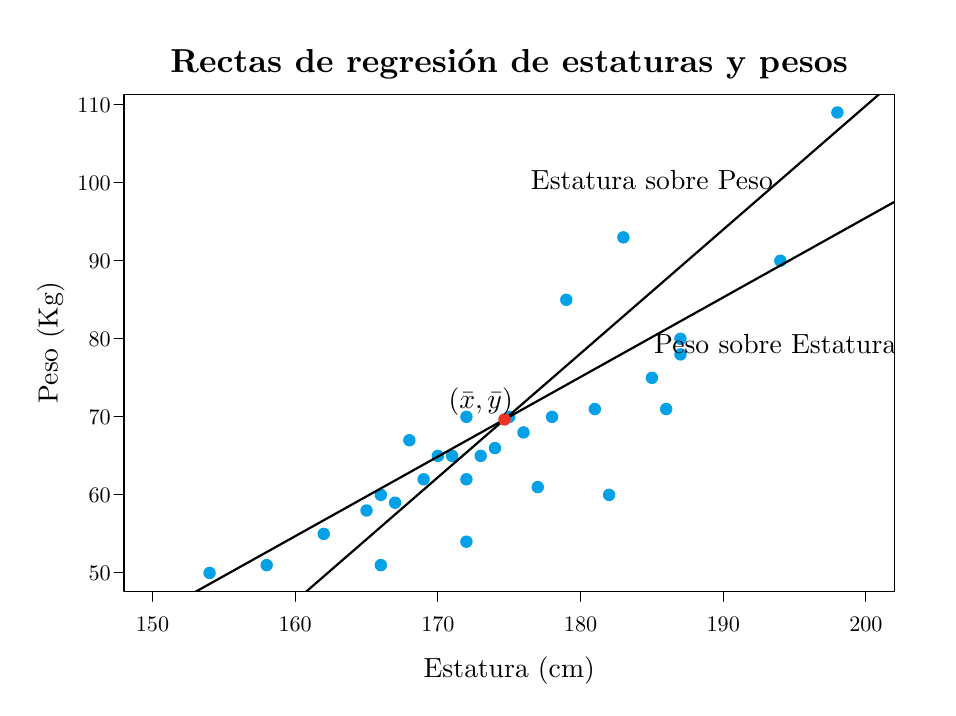
\begin{tikzpicture}[x=1pt,y=1pt]
\definecolor{fillColor}{RGB}{255,255,255}
\path[use as bounding box,fill=fillColor,fill opacity=0.00] (0,0) rectangle (325.21,238.49);
\begin{scope}
\path[clip] ( 34.80, 34.80) rectangle (313.21,214.49);
\definecolor{fillColor}{RGB}{5,161,230}

\path[fill=fillColor] (194.63,140.16) circle (  2.25);

\path[fill=fillColor] (163.70, 83.76) circle (  2.25);

\path[fill=fillColor] (204.94,100.68) circle (  2.25);

\path[fill=fillColor] (148.23, 83.76) circle (  2.25);

\path[fill=fillColor] ( 86.36, 44.28) circle (  2.25);

\path[fill=fillColor] (168.85, 86.58) circle (  2.25);

\path[fill=fillColor] (158.54, 75.30) circle (  2.25);

\path[fill=fillColor] (127.61, 69.66) circle (  2.25);

\path[fill=fillColor] (271.97,154.26) circle (  2.25);

\path[fill=fillColor] (225.57,111.96) circle (  2.25);

\path[fill=fillColor] (106.98, 55.56) circle (  2.25);

\path[fill=fillColor] (235.88,120.42) circle (  2.25);

\path[fill=fillColor] (292.59,207.84) circle (  2.25);

\path[fill=fillColor] (184.32, 72.48) circle (  2.25);

\path[fill=fillColor] (189.48, 97.86) circle (  2.25);

\path[fill=fillColor] (122.45, 64.02) circle (  2.25);

\path[fill=fillColor] ( 65.73, 41.46) circle (  2.25);

\path[fill=fillColor] (215.25,162.72) circle (  2.25);

\path[fill=fillColor] (127.61, 44.28) circle (  2.25);

\path[fill=fillColor] (153.38, 83.76) circle (  2.25);

\path[fill=fillColor] (174.01, 97.86) circle (  2.25);

\path[fill=fillColor] (210.10, 69.66) circle (  2.25);

\path[fill=fillColor] (132.76, 66.84) circle (  2.25);

\path[fill=fillColor] (143.07, 75.30) circle (  2.25);

\path[fill=fillColor] (158.54, 97.86) circle (  2.25);

\path[fill=fillColor] (230.72,100.68) circle (  2.25);

\path[fill=fillColor] (158.54, 52.74) circle (  2.25);

\path[fill=fillColor] (179.16, 92.22) circle (  2.25);

\path[fill=fillColor] (137.92, 89.40) circle (  2.25);

\path[fill=fillColor] (235.88,126.06) circle (  2.25);
\end{scope}
\begin{scope}
\path[clip] (  0.00,  0.00) rectangle (325.21,238.49);
\definecolor{drawColor}{RGB}{0,0,0}

\path[draw=drawColor,line width= 0.4pt,line join=round,line cap=round] ( 45.11, 34.80) -- (302.90, 34.80);

\path[draw=drawColor,line width= 0.4pt,line join=round,line cap=round] ( 45.11, 34.80) -- ( 45.11, 31.21);

\path[draw=drawColor,line width= 0.4pt,line join=round,line cap=round] ( 96.67, 34.80) -- ( 96.67, 31.21);

\path[draw=drawColor,line width= 0.4pt,line join=round,line cap=round] (148.23, 34.80) -- (148.23, 31.21);

\path[draw=drawColor,line width= 0.4pt,line join=round,line cap=round] (199.79, 34.80) -- (199.79, 31.21);

\path[draw=drawColor,line width= 0.4pt,line join=round,line cap=round] (251.34, 34.80) -- (251.34, 31.21);

\path[draw=drawColor,line width= 0.4pt,line join=round,line cap=round] (302.90, 34.80) -- (302.90, 31.21);

\node[text=drawColor,anchor=base,inner sep=0pt, outer sep=0pt, scale=  0.80] at ( 45.11, 20.40) {150};

\node[text=drawColor,anchor=base,inner sep=0pt, outer sep=0pt, scale=  0.80] at ( 96.67, 20.40) {160};

\node[text=drawColor,anchor=base,inner sep=0pt, outer sep=0pt, scale=  0.80] at (148.23, 20.40) {170};

\node[text=drawColor,anchor=base,inner sep=0pt, outer sep=0pt, scale=  0.80] at (199.79, 20.40) {180};

\node[text=drawColor,anchor=base,inner sep=0pt, outer sep=0pt, scale=  0.80] at (251.34, 20.40) {190};

\node[text=drawColor,anchor=base,inner sep=0pt, outer sep=0pt, scale=  0.80] at (302.90, 20.40) {200};

\path[draw=drawColor,line width= 0.4pt,line join=round,line cap=round] ( 34.80, 41.46) -- ( 34.80,210.66);

\path[draw=drawColor,line width= 0.4pt,line join=round,line cap=round] ( 34.80, 41.46) -- ( 31.21, 41.46);

\path[draw=drawColor,line width= 0.4pt,line join=round,line cap=round] ( 34.80, 69.66) -- ( 31.21, 69.66);

\path[draw=drawColor,line width= 0.4pt,line join=round,line cap=round] ( 34.80, 97.86) -- ( 31.21, 97.86);

\path[draw=drawColor,line width= 0.4pt,line join=round,line cap=round] ( 34.80,126.06) -- ( 31.21,126.06);

\path[draw=drawColor,line width= 0.4pt,line join=round,line cap=round] ( 34.80,154.26) -- ( 31.21,154.26);

\path[draw=drawColor,line width= 0.4pt,line join=round,line cap=round] ( 34.80,182.46) -- ( 31.21,182.46);

\path[draw=drawColor,line width= 0.4pt,line join=round,line cap=round] ( 34.80,210.66) -- ( 31.21,210.66);

\node[text=drawColor,anchor=base east,inner sep=0pt, outer sep=0pt, scale=  0.80] at ( 30.00, 38.70) {50};

\node[text=drawColor,anchor=base east,inner sep=0pt, outer sep=0pt, scale=  0.80] at ( 30.00, 66.90) {60};

\node[text=drawColor,anchor=base east,inner sep=0pt, outer sep=0pt, scale=  0.80] at ( 30.00, 95.10) {70};

\node[text=drawColor,anchor=base east,inner sep=0pt, outer sep=0pt, scale=  0.80] at ( 30.00,123.30) {80};

\node[text=drawColor,anchor=base east,inner sep=0pt, outer sep=0pt, scale=  0.80] at ( 30.00,151.50) {90};

\node[text=drawColor,anchor=base east,inner sep=0pt, outer sep=0pt, scale=  0.80] at ( 30.00,179.70) {100};

\node[text=drawColor,anchor=base east,inner sep=0pt, outer sep=0pt, scale=  0.80] at ( 30.00,207.90) {110};

\path[draw=drawColor,line width= 0.4pt,line join=round,line cap=round] ( 34.80, 34.80) --
	(313.21, 34.80) --
	(313.21,214.49) --
	( 34.80,214.49) --
	( 34.80, 34.80);
\end{scope}
\begin{scope}
\path[clip] (  0.00,  0.00) rectangle (325.21,238.49);
\definecolor{drawColor}{RGB}{0,0,0}

\node[text=drawColor,anchor=base,inner sep=0pt, outer sep=0pt, scale=  1.20] at (174.01,222.30) {\bfseries Rectas de regresión de estaturas y pesos};

\node[text=drawColor,anchor=base,inner sep=0pt, outer sep=0pt, scale=  1.00] at (174.01,  3.60) {Estatura (cm)};

\node[text=drawColor,rotate= 90.00,anchor=base,inner sep=0pt, outer sep=0pt, scale=  1.00] at ( 10.80,124.65) {Peso (Kg)};
\end{scope}
\begin{scope}
\path[clip] ( 34.80, 34.80) rectangle (313.21,214.49);
\definecolor{drawColor}{RGB}{0,0,0}

\path[draw=drawColor,line width= 0.8pt,line join=round,line cap=round] ( 34.80, 20.22) -- (313.21,175.55);

\path[draw=drawColor,line width= 0.8pt,line join=round,line cap=round] ( 60.68,  0.00) -- (313.21,219.25);
\definecolor{fillColor}{RGB}{238,50,36}

\path[fill=fillColor] (172.31, 96.92) circle (  2.25);

\node[text=drawColor,anchor=base,inner sep=0pt, outer sep=0pt, scale=  1.00] at (163.70,101.00) {$(\bar x, \bar y)$};

\node[text=drawColor,anchor=base,inner sep=0pt, outer sep=0pt, scale=  1.00] at (270.12,120.58) {Peso sobre Estatura};

\node[text=drawColor,anchor=base,inner sep=0pt, outer sep=0pt, scale=  1.00] at (225.57,179.98) {Estatura sobre Peso};
\end{scope}
\end{tikzpicture}
}}
\mode<presentation>{\resizebox{0.9\textwidth}{!}{% Created by tikzDevice version 0.10.1 on 2016-02-27 13:06:07
% !TEX encoding = UTF-8 Unicode
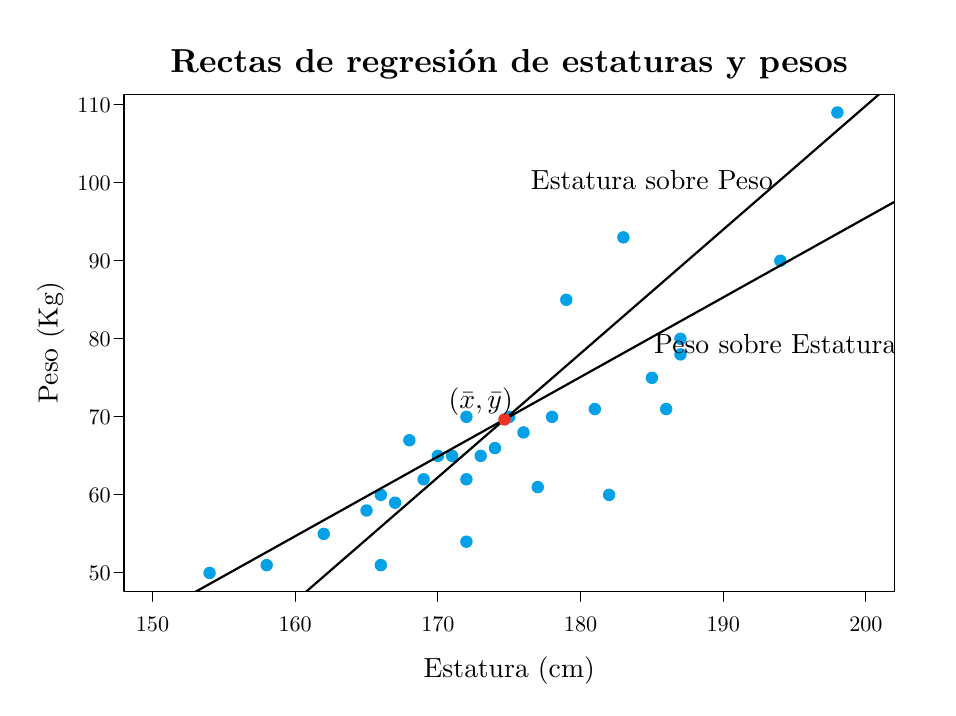
\begin{tikzpicture}[x=1pt,y=1pt]
\definecolor{fillColor}{RGB}{255,255,255}
\path[use as bounding box,fill=fillColor,fill opacity=0.00] (0,0) rectangle (325.21,238.49);
\begin{scope}
\path[clip] ( 34.80, 34.80) rectangle (313.21,214.49);
\definecolor{fillColor}{RGB}{5,161,230}

\path[fill=fillColor] (194.63,140.16) circle (  2.25);

\path[fill=fillColor] (163.70, 83.76) circle (  2.25);

\path[fill=fillColor] (204.94,100.68) circle (  2.25);

\path[fill=fillColor] (148.23, 83.76) circle (  2.25);

\path[fill=fillColor] ( 86.36, 44.28) circle (  2.25);

\path[fill=fillColor] (168.85, 86.58) circle (  2.25);

\path[fill=fillColor] (158.54, 75.30) circle (  2.25);

\path[fill=fillColor] (127.61, 69.66) circle (  2.25);

\path[fill=fillColor] (271.97,154.26) circle (  2.25);

\path[fill=fillColor] (225.57,111.96) circle (  2.25);

\path[fill=fillColor] (106.98, 55.56) circle (  2.25);

\path[fill=fillColor] (235.88,120.42) circle (  2.25);

\path[fill=fillColor] (292.59,207.84) circle (  2.25);

\path[fill=fillColor] (184.32, 72.48) circle (  2.25);

\path[fill=fillColor] (189.48, 97.86) circle (  2.25);

\path[fill=fillColor] (122.45, 64.02) circle (  2.25);

\path[fill=fillColor] ( 65.73, 41.46) circle (  2.25);

\path[fill=fillColor] (215.25,162.72) circle (  2.25);

\path[fill=fillColor] (127.61, 44.28) circle (  2.25);

\path[fill=fillColor] (153.38, 83.76) circle (  2.25);

\path[fill=fillColor] (174.01, 97.86) circle (  2.25);

\path[fill=fillColor] (210.10, 69.66) circle (  2.25);

\path[fill=fillColor] (132.76, 66.84) circle (  2.25);

\path[fill=fillColor] (143.07, 75.30) circle (  2.25);

\path[fill=fillColor] (158.54, 97.86) circle (  2.25);

\path[fill=fillColor] (230.72,100.68) circle (  2.25);

\path[fill=fillColor] (158.54, 52.74) circle (  2.25);

\path[fill=fillColor] (179.16, 92.22) circle (  2.25);

\path[fill=fillColor] (137.92, 89.40) circle (  2.25);

\path[fill=fillColor] (235.88,126.06) circle (  2.25);
\end{scope}
\begin{scope}
\path[clip] (  0.00,  0.00) rectangle (325.21,238.49);
\definecolor{drawColor}{RGB}{0,0,0}

\path[draw=drawColor,line width= 0.4pt,line join=round,line cap=round] ( 45.11, 34.80) -- (302.90, 34.80);

\path[draw=drawColor,line width= 0.4pt,line join=round,line cap=round] ( 45.11, 34.80) -- ( 45.11, 31.21);

\path[draw=drawColor,line width= 0.4pt,line join=round,line cap=round] ( 96.67, 34.80) -- ( 96.67, 31.21);

\path[draw=drawColor,line width= 0.4pt,line join=round,line cap=round] (148.23, 34.80) -- (148.23, 31.21);

\path[draw=drawColor,line width= 0.4pt,line join=round,line cap=round] (199.79, 34.80) -- (199.79, 31.21);

\path[draw=drawColor,line width= 0.4pt,line join=round,line cap=round] (251.34, 34.80) -- (251.34, 31.21);

\path[draw=drawColor,line width= 0.4pt,line join=round,line cap=round] (302.90, 34.80) -- (302.90, 31.21);

\node[text=drawColor,anchor=base,inner sep=0pt, outer sep=0pt, scale=  0.80] at ( 45.11, 20.40) {150};

\node[text=drawColor,anchor=base,inner sep=0pt, outer sep=0pt, scale=  0.80] at ( 96.67, 20.40) {160};

\node[text=drawColor,anchor=base,inner sep=0pt, outer sep=0pt, scale=  0.80] at (148.23, 20.40) {170};

\node[text=drawColor,anchor=base,inner sep=0pt, outer sep=0pt, scale=  0.80] at (199.79, 20.40) {180};

\node[text=drawColor,anchor=base,inner sep=0pt, outer sep=0pt, scale=  0.80] at (251.34, 20.40) {190};

\node[text=drawColor,anchor=base,inner sep=0pt, outer sep=0pt, scale=  0.80] at (302.90, 20.40) {200};

\path[draw=drawColor,line width= 0.4pt,line join=round,line cap=round] ( 34.80, 41.46) -- ( 34.80,210.66);

\path[draw=drawColor,line width= 0.4pt,line join=round,line cap=round] ( 34.80, 41.46) -- ( 31.21, 41.46);

\path[draw=drawColor,line width= 0.4pt,line join=round,line cap=round] ( 34.80, 69.66) -- ( 31.21, 69.66);

\path[draw=drawColor,line width= 0.4pt,line join=round,line cap=round] ( 34.80, 97.86) -- ( 31.21, 97.86);

\path[draw=drawColor,line width= 0.4pt,line join=round,line cap=round] ( 34.80,126.06) -- ( 31.21,126.06);

\path[draw=drawColor,line width= 0.4pt,line join=round,line cap=round] ( 34.80,154.26) -- ( 31.21,154.26);

\path[draw=drawColor,line width= 0.4pt,line join=round,line cap=round] ( 34.80,182.46) -- ( 31.21,182.46);

\path[draw=drawColor,line width= 0.4pt,line join=round,line cap=round] ( 34.80,210.66) -- ( 31.21,210.66);

\node[text=drawColor,anchor=base east,inner sep=0pt, outer sep=0pt, scale=  0.80] at ( 30.00, 38.70) {50};

\node[text=drawColor,anchor=base east,inner sep=0pt, outer sep=0pt, scale=  0.80] at ( 30.00, 66.90) {60};

\node[text=drawColor,anchor=base east,inner sep=0pt, outer sep=0pt, scale=  0.80] at ( 30.00, 95.10) {70};

\node[text=drawColor,anchor=base east,inner sep=0pt, outer sep=0pt, scale=  0.80] at ( 30.00,123.30) {80};

\node[text=drawColor,anchor=base east,inner sep=0pt, outer sep=0pt, scale=  0.80] at ( 30.00,151.50) {90};

\node[text=drawColor,anchor=base east,inner sep=0pt, outer sep=0pt, scale=  0.80] at ( 30.00,179.70) {100};

\node[text=drawColor,anchor=base east,inner sep=0pt, outer sep=0pt, scale=  0.80] at ( 30.00,207.90) {110};

\path[draw=drawColor,line width= 0.4pt,line join=round,line cap=round] ( 34.80, 34.80) --
	(313.21, 34.80) --
	(313.21,214.49) --
	( 34.80,214.49) --
	( 34.80, 34.80);
\end{scope}
\begin{scope}
\path[clip] (  0.00,  0.00) rectangle (325.21,238.49);
\definecolor{drawColor}{RGB}{0,0,0}

\node[text=drawColor,anchor=base,inner sep=0pt, outer sep=0pt, scale=  1.20] at (174.01,222.30) {\bfseries Rectas de regresión de estaturas y pesos};

\node[text=drawColor,anchor=base,inner sep=0pt, outer sep=0pt, scale=  1.00] at (174.01,  3.60) {Estatura (cm)};

\node[text=drawColor,rotate= 90.00,anchor=base,inner sep=0pt, outer sep=0pt, scale=  1.00] at ( 10.80,124.65) {Peso (Kg)};
\end{scope}
\begin{scope}
\path[clip] ( 34.80, 34.80) rectangle (313.21,214.49);
\definecolor{drawColor}{RGB}{0,0,0}

\path[draw=drawColor,line width= 0.8pt,line join=round,line cap=round] ( 34.80, 20.22) -- (313.21,175.55);

\path[draw=drawColor,line width= 0.8pt,line join=round,line cap=round] ( 60.68,  0.00) -- (313.21,219.25);
\definecolor{fillColor}{RGB}{238,50,36}

\path[fill=fillColor] (172.31, 96.92) circle (  2.25);

\node[text=drawColor,anchor=base,inner sep=0pt, outer sep=0pt, scale=  1.00] at (163.70,101.00) {$(\bar x, \bar y)$};

\node[text=drawColor,anchor=base,inner sep=0pt, outer sep=0pt, scale=  1.00] at (270.12,120.58) {Peso sobre Estatura};

\node[text=drawColor,anchor=base,inner sep=0pt, outer sep=0pt, scale=  1.00] at (225.57,179.98) {Estatura sobre Peso};
\end{scope}
\end{tikzpicture}
}}
\end{center}

\note{Si dibujamos ambas rectas, la del peso sobre la estatura y la de la estatura sobre el peso, podemos comprobar que se trata de rectas
distintas, ya que la primera hace mínimos los residuos del peso, y por tanto es la que debe utilizarse para predecir el peso en función de
la estatura, mientras que la segunda es la que hace mínimos los residuos de la estatura, y por tanto debe utilizarse para predecir la
estatura en función del peso.

Además puede comprobarse que las rectas de regresión se cortan en el punto de medias, lo cual se deduce fácilmente de sus respectivas
ecuaciones.
}
\end{frame}


%---------------------------------------------------------------------slide----
\begin{frame}
\frametitle{Posición relativa de las rectas de regresión}
Habitualmente, las rectas de regresión $Y$ sobre $X$ y de $X$
sobre $Y$ no coinciden, pero siempre se cortan en el punto de medias $(\bar x,\bar y)$.

\begin{columns}
\begin{column}{0.48\textwidth}
Si entre las variables la relación lineal es perfecta, entonces ambas rectas coinciden ya que sus residuos son nulos.
\begin{center}
\tikzsetnextfilename{regresion/regresion_lineal_perfecta}
\mode<article>{\resizebox{0.6\textwidth}{!}{% Created by tikzDevice version 0.10.1 on 2016-02-27 13:20:05
% !TEX encoding = UTF-8 Unicode
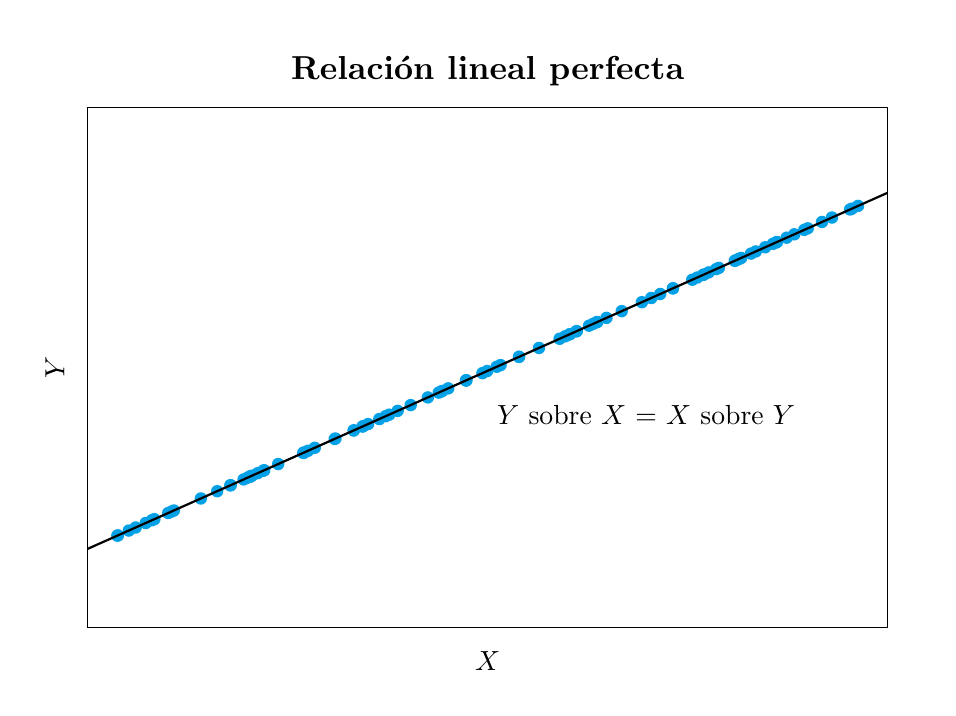
\begin{tikzpicture}[x=1pt,y=1pt]
\definecolor{fillColor}{RGB}{255,255,255}
\path[use as bounding box,fill=fillColor,fill opacity=0.00] (0,0) rectangle (325.21,238.49);
\begin{scope}
\path[clip] ( 21.68, 21.68) rectangle (310.76,209.58);
\definecolor{fillColor}{RGB}{5,161,230}

\path[fill=fillColor] (170.88,116.57) circle (  2.25);

\path[fill=fillColor] (177.53,119.53) circle (  2.25);

\path[fill=fillColor] ( 50.79, 63.12) circle (  2.25);

\path[fill=fillColor] ( 32.62, 55.02) circle (  2.25);

\path[fill=fillColor] (111.23, 90.02) circle (  2.25);

\path[fill=fillColor] (246.09,150.05) circle (  2.25);

\path[fill=fillColor] (266.49,159.13) circle (  2.25);

\path[fill=fillColor] (255.80,154.38) circle (  2.25);

\path[fill=fillColor] (148.53,106.62) circle (  2.25);

\path[fill=fillColor] ( 62.58, 68.36) circle (  2.25);

\path[fill=fillColor] ( 32.39, 54.92) circle (  2.25);

\path[fill=fillColor] ( 80.30, 76.25) circle (  2.25);

\path[fill=fillColor] (198.23,128.75) circle (  2.25);

\path[fill=fillColor] (228.57,142.26) circle (  2.25);

\path[fill=fillColor] (297.17,172.79) circle (  2.25);

\path[fill=fillColor] (101.29, 85.59) circle (  2.25);

\path[fill=fillColor] (184.76,122.75) circle (  2.25);

\path[fill=fillColor] (127.05, 97.06) circle (  2.25);

\path[fill=fillColor] (209.14,133.61) circle (  2.25);

\path[fill=fillColor] ( 99.88, 84.97) circle (  2.25);

\path[fill=fillColor] (277.02,163.82) circle (  2.25);

\path[fill=fillColor] ( 83.08, 77.49) circle (  2.25);

\path[fill=fillColor] (133.69,100.02) circle (  2.25);

\path[fill=fillColor] (123.00, 95.26) circle (  2.25);

\path[fill=fillColor] ( 52.00, 63.65) circle (  2.25);

\path[fill=fillColor] (202.86,130.81) circle (  2.25);

\path[fill=fillColor] (221.94,139.30) circle (  2.25);

\path[fill=fillColor] (255.50,154.24) circle (  2.25);

\path[fill=fillColor] (300.05,174.08) circle (  2.25);

\path[fill=fillColor] (164.33,113.66) circle (  2.25);

\path[fill=fillColor] (204.32,131.46) circle (  2.25);

\path[fill=fillColor] ( 45.77, 60.88) circle (  2.25);

\path[fill=fillColor] ( 80.54, 76.36) circle (  2.25);

\path[fill=fillColor] (257.83,155.28) circle (  2.25);

\path[fill=fillColor] ( 78.03, 75.24) circle (  2.25);

\path[fill=fillColor] (248.79,151.25) circle (  2.25);

\path[fill=fillColor] (270.78,161.04) circle (  2.25);

\path[fill=fillColor] (129.34, 98.08) circle (  2.25);

\path[fill=fillColor] (280.63,165.43) circle (  2.25);

\path[fill=fillColor] (195.95,127.73) circle (  2.25);

\path[fill=fillColor] (192.21,126.07) circle (  2.25);

\path[fill=fillColor] ( 52.84, 64.02) circle (  2.25);

\path[fill=fillColor] (151.97,108.15) circle (  2.25);

\path[fill=fillColor] (158.55,111.08) circle (  2.25);

\path[fill=fillColor] (256.72,154.79) circle (  2.25);

\path[fill=fillColor] (297.87,173.10) circle (  2.25);

\path[fill=fillColor] (263.10,157.63) circle (  2.25);

\path[fill=fillColor] ( 99.60, 84.84) circle (  2.25);

\path[fill=fillColor] ( 42.65, 59.49) circle (  2.25);

\path[fill=fillColor] (257.02,154.92) circle (  2.25);

\path[fill=fillColor] ( 79.42, 75.86) circle (  2.25);

\path[fill=fillColor] (225.33,140.81) circle (  2.25);

\path[fill=fillColor] ( 36.54, 56.77) circle (  2.25);

\path[fill=fillColor] ( 85.08, 78.38) circle (  2.25);

\path[fill=fillColor] (244.03,149.14) circle (  2.25);

\path[fill=fillColor] (158.39,111.01) circle (  2.25);

\path[fill=fillColor] ( 39.03, 57.88) circle (  2.25);

\path[fill=fillColor] (130.61, 98.64) circle (  2.25);

\path[fill=fillColor] (117.88, 92.98) circle (  2.25);

\path[fill=fillColor] (149.86,107.22) circle (  2.25);

\path[fill=fillColor] (261.37,156.85) circle (  2.25);

\path[fill=fillColor] (144.60,104.88) circle (  2.25);

\path[fill=fillColor] (205.84,132.14) circle (  2.25);

\path[fill=fillColor] (117.77, 92.93) circle (  2.25);

\path[fill=fillColor] (194.22,126.96) circle (  2.25);

\path[fill=fillColor] ( 68.49, 70.99) circle (  2.25);

\path[fill=fillColor] (198.43,128.84) circle (  2.25);

\path[fill=fillColor] (121.26, 94.49) circle (  2.25);

\path[fill=fillColor] (270.34,160.85) circle (  2.25);

\path[fill=fillColor] (233.15,144.29) circle (  2.25);

\path[fill=fillColor] ( 73.22, 73.10) circle (  2.25);

\path[fill=fillColor] (249.77,151.69) circle (  2.25);

\path[fill=fillColor] (103.73, 86.68) circle (  2.25);

\path[fill=fillColor] (120.96, 94.35) circle (  2.25);

\path[fill=fillColor] ( 80.43, 76.31) circle (  2.25);

\path[fill=fillColor] ( 85.48, 78.56) circle (  2.25);

\path[fill=fillColor] (214.66,136.06) circle (  2.25);

\path[fill=fillColor] ( 99.68, 84.88) circle (  2.25);

\path[fill=fillColor] (241.94,148.21) circle (  2.25);

\path[fill=fillColor] (281.87,165.98) circle (  2.25);

\path[fill=fillColor] ( 44.88, 60.48) circle (  2.25);

\path[fill=fillColor] (195.76,127.65) circle (  2.25);

\path[fill=fillColor] ( 81.05, 76.59) circle (  2.25);

\path[fill=fillColor] ( 90.53, 80.81) circle (  2.25);

\path[fill=fillColor] (290.62,169.88) circle (  2.25);

\path[fill=fillColor] (158.42,111.03) circle (  2.25);

\path[fill=fillColor] (177.57,119.55) circle (  2.25);

\path[fill=fillColor] (205.60,132.03) circle (  2.25);

\path[fill=fillColor] (110.95, 89.89) circle (  2.25);

\path[fill=fillColor] (138.40,102.11) circle (  2.25);

\path[fill=fillColor] ( 73.37, 73.17) circle (  2.25);

\path[fill=fillColor] (233.18,144.31) circle (  2.25);

\path[fill=fillColor] (240.15,147.41) circle (  2.25);

\path[fill=fillColor] (244.40,149.30) circle (  2.25);

\path[fill=fillColor] (149.31,106.97) circle (  2.25);

\path[fill=fillColor] (166.05,114.42) circle (  2.25);

\path[fill=fillColor] (274.27,162.60) circle (  2.25);

\path[fill=fillColor] (287.03,168.28) circle (  2.25);

\path[fill=fillColor] (169.50,115.96) circle (  2.25);

\path[fill=fillColor] (269.30,160.39) circle (  2.25);
\end{scope}
\begin{scope}
\path[clip] (  0.00,  0.00) rectangle (325.21,238.49);
\definecolor{drawColor}{RGB}{0,0,0}

\node[text=drawColor,anchor=base,inner sep=0pt, outer sep=0pt, scale=  1.20] at (166.22,219.84) {\bfseries Relación lineal perfecta};

\node[text=drawColor,anchor=base,inner sep=0pt, outer sep=0pt, scale=  1.00] at (166.22,  6.08) {$X$};

\node[text=drawColor,rotate= 90.00,anchor=base,inner sep=0pt, outer sep=0pt, scale=  1.00] at ( 13.28,115.63) {$Y$};
\end{scope}
\begin{scope}
\path[clip] (  0.00,  0.00) rectangle (325.21,238.49);
\definecolor{drawColor}{RGB}{0,0,0}

\path[draw=drawColor,line width= 0.4pt,line join=round,line cap=round] ( 21.68, 21.68) --
	(310.76, 21.68) --
	(310.76,209.58) --
	( 21.68,209.58) --
	( 21.68, 21.68);
\end{scope}
\begin{scope}
\path[clip] ( 21.68, 21.68) rectangle (310.76,209.58);
\definecolor{drawColor}{RGB}{0,0,0}

\path[draw=drawColor,line width= 0.8pt,line join=round,line cap=round] ( 21.68, 50.16) -- (310.76,178.84);

\node[text=drawColor,anchor=base,inner sep=0pt, outer sep=0pt, scale=  1.00] at (223.48, 94.97) {$Y$ sobre $X$ = $X$ sobre $Y$};
\end{scope}
\end{tikzpicture}
}}
\mode<presentation>{\resizebox{0.9\textwidth}{!}{% Created by tikzDevice version 0.10.1 on 2016-02-27 13:20:05
% !TEX encoding = UTF-8 Unicode
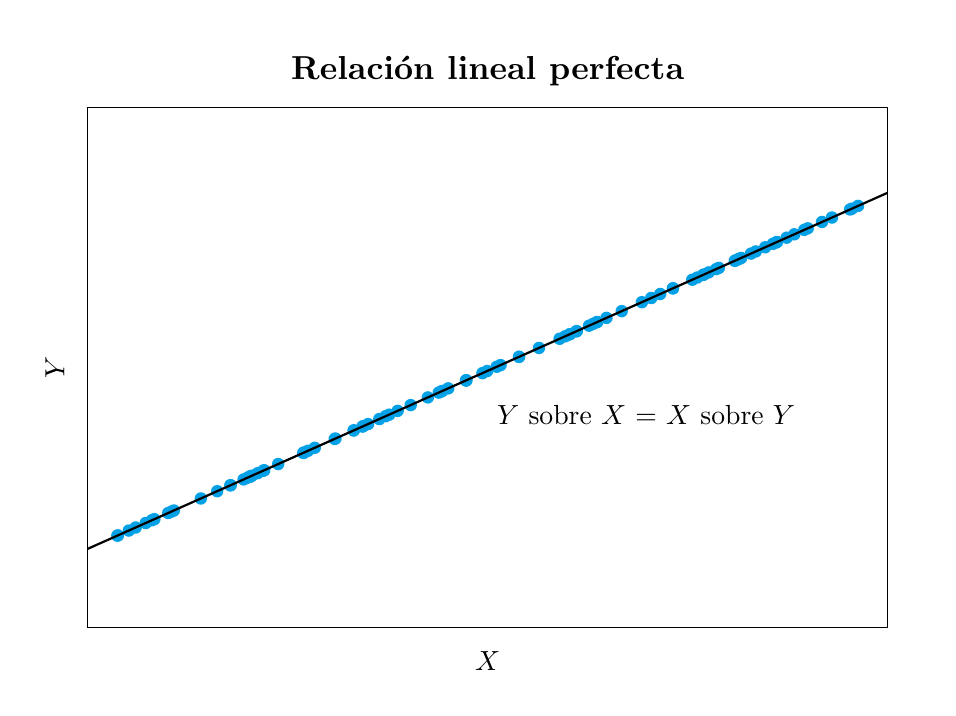
\begin{tikzpicture}[x=1pt,y=1pt]
\definecolor{fillColor}{RGB}{255,255,255}
\path[use as bounding box,fill=fillColor,fill opacity=0.00] (0,0) rectangle (325.21,238.49);
\begin{scope}
\path[clip] ( 21.68, 21.68) rectangle (310.76,209.58);
\definecolor{fillColor}{RGB}{5,161,230}

\path[fill=fillColor] (170.88,116.57) circle (  2.25);

\path[fill=fillColor] (177.53,119.53) circle (  2.25);

\path[fill=fillColor] ( 50.79, 63.12) circle (  2.25);

\path[fill=fillColor] ( 32.62, 55.02) circle (  2.25);

\path[fill=fillColor] (111.23, 90.02) circle (  2.25);

\path[fill=fillColor] (246.09,150.05) circle (  2.25);

\path[fill=fillColor] (266.49,159.13) circle (  2.25);

\path[fill=fillColor] (255.80,154.38) circle (  2.25);

\path[fill=fillColor] (148.53,106.62) circle (  2.25);

\path[fill=fillColor] ( 62.58, 68.36) circle (  2.25);

\path[fill=fillColor] ( 32.39, 54.92) circle (  2.25);

\path[fill=fillColor] ( 80.30, 76.25) circle (  2.25);

\path[fill=fillColor] (198.23,128.75) circle (  2.25);

\path[fill=fillColor] (228.57,142.26) circle (  2.25);

\path[fill=fillColor] (297.17,172.79) circle (  2.25);

\path[fill=fillColor] (101.29, 85.59) circle (  2.25);

\path[fill=fillColor] (184.76,122.75) circle (  2.25);

\path[fill=fillColor] (127.05, 97.06) circle (  2.25);

\path[fill=fillColor] (209.14,133.61) circle (  2.25);

\path[fill=fillColor] ( 99.88, 84.97) circle (  2.25);

\path[fill=fillColor] (277.02,163.82) circle (  2.25);

\path[fill=fillColor] ( 83.08, 77.49) circle (  2.25);

\path[fill=fillColor] (133.69,100.02) circle (  2.25);

\path[fill=fillColor] (123.00, 95.26) circle (  2.25);

\path[fill=fillColor] ( 52.00, 63.65) circle (  2.25);

\path[fill=fillColor] (202.86,130.81) circle (  2.25);

\path[fill=fillColor] (221.94,139.30) circle (  2.25);

\path[fill=fillColor] (255.50,154.24) circle (  2.25);

\path[fill=fillColor] (300.05,174.08) circle (  2.25);

\path[fill=fillColor] (164.33,113.66) circle (  2.25);

\path[fill=fillColor] (204.32,131.46) circle (  2.25);

\path[fill=fillColor] ( 45.77, 60.88) circle (  2.25);

\path[fill=fillColor] ( 80.54, 76.36) circle (  2.25);

\path[fill=fillColor] (257.83,155.28) circle (  2.25);

\path[fill=fillColor] ( 78.03, 75.24) circle (  2.25);

\path[fill=fillColor] (248.79,151.25) circle (  2.25);

\path[fill=fillColor] (270.78,161.04) circle (  2.25);

\path[fill=fillColor] (129.34, 98.08) circle (  2.25);

\path[fill=fillColor] (280.63,165.43) circle (  2.25);

\path[fill=fillColor] (195.95,127.73) circle (  2.25);

\path[fill=fillColor] (192.21,126.07) circle (  2.25);

\path[fill=fillColor] ( 52.84, 64.02) circle (  2.25);

\path[fill=fillColor] (151.97,108.15) circle (  2.25);

\path[fill=fillColor] (158.55,111.08) circle (  2.25);

\path[fill=fillColor] (256.72,154.79) circle (  2.25);

\path[fill=fillColor] (297.87,173.10) circle (  2.25);

\path[fill=fillColor] (263.10,157.63) circle (  2.25);

\path[fill=fillColor] ( 99.60, 84.84) circle (  2.25);

\path[fill=fillColor] ( 42.65, 59.49) circle (  2.25);

\path[fill=fillColor] (257.02,154.92) circle (  2.25);

\path[fill=fillColor] ( 79.42, 75.86) circle (  2.25);

\path[fill=fillColor] (225.33,140.81) circle (  2.25);

\path[fill=fillColor] ( 36.54, 56.77) circle (  2.25);

\path[fill=fillColor] ( 85.08, 78.38) circle (  2.25);

\path[fill=fillColor] (244.03,149.14) circle (  2.25);

\path[fill=fillColor] (158.39,111.01) circle (  2.25);

\path[fill=fillColor] ( 39.03, 57.88) circle (  2.25);

\path[fill=fillColor] (130.61, 98.64) circle (  2.25);

\path[fill=fillColor] (117.88, 92.98) circle (  2.25);

\path[fill=fillColor] (149.86,107.22) circle (  2.25);

\path[fill=fillColor] (261.37,156.85) circle (  2.25);

\path[fill=fillColor] (144.60,104.88) circle (  2.25);

\path[fill=fillColor] (205.84,132.14) circle (  2.25);

\path[fill=fillColor] (117.77, 92.93) circle (  2.25);

\path[fill=fillColor] (194.22,126.96) circle (  2.25);

\path[fill=fillColor] ( 68.49, 70.99) circle (  2.25);

\path[fill=fillColor] (198.43,128.84) circle (  2.25);

\path[fill=fillColor] (121.26, 94.49) circle (  2.25);

\path[fill=fillColor] (270.34,160.85) circle (  2.25);

\path[fill=fillColor] (233.15,144.29) circle (  2.25);

\path[fill=fillColor] ( 73.22, 73.10) circle (  2.25);

\path[fill=fillColor] (249.77,151.69) circle (  2.25);

\path[fill=fillColor] (103.73, 86.68) circle (  2.25);

\path[fill=fillColor] (120.96, 94.35) circle (  2.25);

\path[fill=fillColor] ( 80.43, 76.31) circle (  2.25);

\path[fill=fillColor] ( 85.48, 78.56) circle (  2.25);

\path[fill=fillColor] (214.66,136.06) circle (  2.25);

\path[fill=fillColor] ( 99.68, 84.88) circle (  2.25);

\path[fill=fillColor] (241.94,148.21) circle (  2.25);

\path[fill=fillColor] (281.87,165.98) circle (  2.25);

\path[fill=fillColor] ( 44.88, 60.48) circle (  2.25);

\path[fill=fillColor] (195.76,127.65) circle (  2.25);

\path[fill=fillColor] ( 81.05, 76.59) circle (  2.25);

\path[fill=fillColor] ( 90.53, 80.81) circle (  2.25);

\path[fill=fillColor] (290.62,169.88) circle (  2.25);

\path[fill=fillColor] (158.42,111.03) circle (  2.25);

\path[fill=fillColor] (177.57,119.55) circle (  2.25);

\path[fill=fillColor] (205.60,132.03) circle (  2.25);

\path[fill=fillColor] (110.95, 89.89) circle (  2.25);

\path[fill=fillColor] (138.40,102.11) circle (  2.25);

\path[fill=fillColor] ( 73.37, 73.17) circle (  2.25);

\path[fill=fillColor] (233.18,144.31) circle (  2.25);

\path[fill=fillColor] (240.15,147.41) circle (  2.25);

\path[fill=fillColor] (244.40,149.30) circle (  2.25);

\path[fill=fillColor] (149.31,106.97) circle (  2.25);

\path[fill=fillColor] (166.05,114.42) circle (  2.25);

\path[fill=fillColor] (274.27,162.60) circle (  2.25);

\path[fill=fillColor] (287.03,168.28) circle (  2.25);

\path[fill=fillColor] (169.50,115.96) circle (  2.25);

\path[fill=fillColor] (269.30,160.39) circle (  2.25);
\end{scope}
\begin{scope}
\path[clip] (  0.00,  0.00) rectangle (325.21,238.49);
\definecolor{drawColor}{RGB}{0,0,0}

\node[text=drawColor,anchor=base,inner sep=0pt, outer sep=0pt, scale=  1.20] at (166.22,219.84) {\bfseries Relación lineal perfecta};

\node[text=drawColor,anchor=base,inner sep=0pt, outer sep=0pt, scale=  1.00] at (166.22,  6.08) {$X$};

\node[text=drawColor,rotate= 90.00,anchor=base,inner sep=0pt, outer sep=0pt, scale=  1.00] at ( 13.28,115.63) {$Y$};
\end{scope}
\begin{scope}
\path[clip] (  0.00,  0.00) rectangle (325.21,238.49);
\definecolor{drawColor}{RGB}{0,0,0}

\path[draw=drawColor,line width= 0.4pt,line join=round,line cap=round] ( 21.68, 21.68) --
	(310.76, 21.68) --
	(310.76,209.58) --
	( 21.68,209.58) --
	( 21.68, 21.68);
\end{scope}
\begin{scope}
\path[clip] ( 21.68, 21.68) rectangle (310.76,209.58);
\definecolor{drawColor}{RGB}{0,0,0}

\path[draw=drawColor,line width= 0.8pt,line join=round,line cap=round] ( 21.68, 50.16) -- (310.76,178.84);

\node[text=drawColor,anchor=base,inner sep=0pt, outer sep=0pt, scale=  1.00] at (223.48, 94.97) {$Y$ sobre $X$ = $X$ sobre $Y$};
\end{scope}
\end{tikzpicture}
}}
\end{center}
\end{column}
\begin{column}{0.48\textwidth}
Si no hay relación lineal, entonces las ecuaciones de las rectas son\\
\qquad \qquad $y = \bar y$, \qquad $x = \bar x,$\\
y se cortan perpendicularmente  
\begin{center}
\tikzsetnextfilename{regresion/rectas_independencia_lineal}
\mode<article>{\resizebox{0.6\textwidth}{!}{%% Input file name: rectas_independencia_lineal.fig
%% FIG version: 3.2
%% Orientation: Landscape
%% Justification: Flush Left
%% Units: Inches
%% Paper size: A4
%% Magnification: 100.0
%% Resolution: 1200ppi
%% Include the following in the preamble:
%% \usepackage{textcomp}
%% End

\begin{pspicture}(7.06cm,3.29cm)(16.36cm,13.56cm)
\psset{unit=0.8cm}
%%
%% Depth: 2147483647
%%
\newrgbcolor{mycolor0}{1.00 0.50 0.31}\definecolor{mycolor0}{rgb}{1.00,0.50,0.31}
%%
%% Depth: 100
%%
\psset{linestyle=solid,linewidth=0.03175,linecolor=mycolor0}
\qdisk(16.63,9.96){0.1}
\qdisk(18.53,10.92){0.1}
\qdisk(13.60,12.64){0.1}
\qdisk(12.83,13.91){0.1}
\qdisk(16.21,6.16){0.1}
\qdisk(16.04,9.07){0.1}
\qdisk(17.89,6.74){0.1}
\qdisk(13.39,11.97){0.1}
\qdisk(13.66,9.79){0.1}
\qdisk(18.77,11.43){0.1}
\qdisk(18.79,10.20){0.1}
\qdisk(15.90,13.76){0.1}
\qdisk(16.33,11.13){0.1}
\qdisk(18.47,9.84){0.1}
\qdisk(11.42,6.20){0.1}
\qdisk(10.15,9.35){0.1}
\qdisk(15.48,12.85){0.1}
\qdisk(12.40,9.99){0.1}
\qdisk(13.81,13.59){0.1}
\qdisk(17.18,6.11){0.1}
\qdisk(17.94,8.41){0.1}
\qdisk(17.76,13.78){0.1}
\qdisk(13.97,8.58){0.1}
\qdisk(18.60,5.92){0.1}
\qdisk(10.92,14.58){0.1}
\qdisk(16.44,12.66){0.1}
\qdisk(18.74,14.83){0.1}
\qdisk(12.98,11.21){0.1}
\qdisk(10.70,8.89){0.1}
\qdisk(10.33,7.27){0.1}
\qdisk(17.96,11.10){0.1}
\qdisk(12.36,15.04){0.1}
\qdisk(17.98,13.34){0.1}
\qdisk(19.55,8.17){0.1}
\qdisk(10.25,6.88){0.1}
\qdisk(12.06,15.26){0.1}
\qdisk(15.21,8.56){0.1}
\qdisk(11.72,8.30){0.1}
\qdisk(12.25,10.12){0.1}
\qdisk(12.58,12.44){0.1}
\qdisk(11.91,12.42){0.1}
\qdisk(14.86,11.21){0.1}
\qdisk(13.75,13.21){0.1}
\qdisk(15.09,15.10){0.1}
\qdisk(12.35,7.22){0.1}
\qdisk(10.73,9.81){0.1}
\qdisk(10.43,14.15){0.1}
\qdisk(11.32,8.59){0.1}
\qdisk(16.15,12.81){0.1}
\qdisk(19.51,7.91){0.1}
\qdisk(11.44,13.64){0.1}
\qdisk(11.21,12.44){0.1}
\qdisk(18.86,6.46){0.1}
\qdisk(10.31,10.08){0.1}
\qdisk(14.02,13.31){0.1}
\qdisk(17.26,8.80){0.1}
\qdisk(13.32,8.87){0.1}
\qdisk(11.63,6.47){0.1}
\qdisk(18.64,9.07){0.1}
\qdisk(11.00,7.62){0.1}
\qdisk(11.52,5.85){0.1}
\qdisk(15.30,7.81){0.1}
\qdisk(10.55,6.39){0.1}
\qdisk(17.38,12.21){0.1}
\qdisk(15.61,13.11){0.1}
\qdisk(10.75,12.83){0.1}
\qdisk(12.50,8.51){0.1}
\qdisk(17.62,13.47){0.1}
\qdisk(12.53,11.83){0.1}
\qdisk(12.42,6.73){0.1}
\qdisk(16.71,12.34){0.1}
\qdisk(13.96,13.40){0.1}
\qdisk(12.70,14.84){0.1}
\qdisk(18.84,8.00){0.1}
\qdisk(10.69,9.75){0.1}
\qdisk(14.34,8.62){0.1}
\qdisk(18.00,11.21){0.1}
\qdisk(14.23,6.39){0.1}
\qdisk(11.13,8.85){0.1}
\qdisk(16.74,7.02){0.1}
\qdisk(13.69,13.22){0.1}
\qdisk(11.43,10.96){0.1}
\qdisk(14.30,6.05){0.1}
\qdisk(18.77,13.78){0.1}
\qdisk(12.15,6.08){0.1}
\qdisk(10.41,12.01){0.1}
\qdisk(16.28,10.93){0.1}
\qdisk(19.51,12.10){0.1}
\qdisk(10.27,7.83){0.1}
\qdisk(17.47,8.75){0.1}
\qdisk(15.26,9.19){0.1}
\qdisk(17.82,6.24){0.1}
\qdisk(16.99,15.21){0.1}
\qdisk(10.35,7.39){0.1}
\qdisk(15.29,8.17){0.1}
\qdisk(19.06,6.05){0.1}
\qdisk(17.96,8.48){0.1}
\qdisk(15.95,8.06){0.1}
\qdisk(15.13,6.57){0.1}
\qdisk(14.13,10.01){0.1}
\rput(14.85,16.12){Sin relación lineal}
\rput[l](14.71,4.63){$X$}
\rput[l]{90}(9.35,10.42){$Y$}
\psset{linecolor=black,fillstyle=none}
\psline(9.77,5.48)(19.93,5.48)(19.93,15.64)(9.77,15.64)(9.77,5.48)
\psset{linewidth=0.0635}
\psline(9.77,10.16)(19.93,10.16)
\psline(14.57,5.48)(14.57,15.64)
\rput[l](14.72,6.85){$X$ sobre $Y$}
\rput[l](17.82,9.57){$Y$ sobre $X$}
\end{pspicture}
%% End
}}
\mode<presentation>{\resizebox{0.9\textwidth}{!}{%% Input file name: rectas_independencia_lineal.fig
%% FIG version: 3.2
%% Orientation: Landscape
%% Justification: Flush Left
%% Units: Inches
%% Paper size: A4
%% Magnification: 100.0
%% Resolution: 1200ppi
%% Include the following in the preamble:
%% \usepackage{textcomp}
%% End

\begin{pspicture}(7.06cm,3.29cm)(16.36cm,13.56cm)
\psset{unit=0.8cm}
%%
%% Depth: 2147483647
%%
\newrgbcolor{mycolor0}{1.00 0.50 0.31}\definecolor{mycolor0}{rgb}{1.00,0.50,0.31}
%%
%% Depth: 100
%%
\psset{linestyle=solid,linewidth=0.03175,linecolor=mycolor0}
\qdisk(16.63,9.96){0.1}
\qdisk(18.53,10.92){0.1}
\qdisk(13.60,12.64){0.1}
\qdisk(12.83,13.91){0.1}
\qdisk(16.21,6.16){0.1}
\qdisk(16.04,9.07){0.1}
\qdisk(17.89,6.74){0.1}
\qdisk(13.39,11.97){0.1}
\qdisk(13.66,9.79){0.1}
\qdisk(18.77,11.43){0.1}
\qdisk(18.79,10.20){0.1}
\qdisk(15.90,13.76){0.1}
\qdisk(16.33,11.13){0.1}
\qdisk(18.47,9.84){0.1}
\qdisk(11.42,6.20){0.1}
\qdisk(10.15,9.35){0.1}
\qdisk(15.48,12.85){0.1}
\qdisk(12.40,9.99){0.1}
\qdisk(13.81,13.59){0.1}
\qdisk(17.18,6.11){0.1}
\qdisk(17.94,8.41){0.1}
\qdisk(17.76,13.78){0.1}
\qdisk(13.97,8.58){0.1}
\qdisk(18.60,5.92){0.1}
\qdisk(10.92,14.58){0.1}
\qdisk(16.44,12.66){0.1}
\qdisk(18.74,14.83){0.1}
\qdisk(12.98,11.21){0.1}
\qdisk(10.70,8.89){0.1}
\qdisk(10.33,7.27){0.1}
\qdisk(17.96,11.10){0.1}
\qdisk(12.36,15.04){0.1}
\qdisk(17.98,13.34){0.1}
\qdisk(19.55,8.17){0.1}
\qdisk(10.25,6.88){0.1}
\qdisk(12.06,15.26){0.1}
\qdisk(15.21,8.56){0.1}
\qdisk(11.72,8.30){0.1}
\qdisk(12.25,10.12){0.1}
\qdisk(12.58,12.44){0.1}
\qdisk(11.91,12.42){0.1}
\qdisk(14.86,11.21){0.1}
\qdisk(13.75,13.21){0.1}
\qdisk(15.09,15.10){0.1}
\qdisk(12.35,7.22){0.1}
\qdisk(10.73,9.81){0.1}
\qdisk(10.43,14.15){0.1}
\qdisk(11.32,8.59){0.1}
\qdisk(16.15,12.81){0.1}
\qdisk(19.51,7.91){0.1}
\qdisk(11.44,13.64){0.1}
\qdisk(11.21,12.44){0.1}
\qdisk(18.86,6.46){0.1}
\qdisk(10.31,10.08){0.1}
\qdisk(14.02,13.31){0.1}
\qdisk(17.26,8.80){0.1}
\qdisk(13.32,8.87){0.1}
\qdisk(11.63,6.47){0.1}
\qdisk(18.64,9.07){0.1}
\qdisk(11.00,7.62){0.1}
\qdisk(11.52,5.85){0.1}
\qdisk(15.30,7.81){0.1}
\qdisk(10.55,6.39){0.1}
\qdisk(17.38,12.21){0.1}
\qdisk(15.61,13.11){0.1}
\qdisk(10.75,12.83){0.1}
\qdisk(12.50,8.51){0.1}
\qdisk(17.62,13.47){0.1}
\qdisk(12.53,11.83){0.1}
\qdisk(12.42,6.73){0.1}
\qdisk(16.71,12.34){0.1}
\qdisk(13.96,13.40){0.1}
\qdisk(12.70,14.84){0.1}
\qdisk(18.84,8.00){0.1}
\qdisk(10.69,9.75){0.1}
\qdisk(14.34,8.62){0.1}
\qdisk(18.00,11.21){0.1}
\qdisk(14.23,6.39){0.1}
\qdisk(11.13,8.85){0.1}
\qdisk(16.74,7.02){0.1}
\qdisk(13.69,13.22){0.1}
\qdisk(11.43,10.96){0.1}
\qdisk(14.30,6.05){0.1}
\qdisk(18.77,13.78){0.1}
\qdisk(12.15,6.08){0.1}
\qdisk(10.41,12.01){0.1}
\qdisk(16.28,10.93){0.1}
\qdisk(19.51,12.10){0.1}
\qdisk(10.27,7.83){0.1}
\qdisk(17.47,8.75){0.1}
\qdisk(15.26,9.19){0.1}
\qdisk(17.82,6.24){0.1}
\qdisk(16.99,15.21){0.1}
\qdisk(10.35,7.39){0.1}
\qdisk(15.29,8.17){0.1}
\qdisk(19.06,6.05){0.1}
\qdisk(17.96,8.48){0.1}
\qdisk(15.95,8.06){0.1}
\qdisk(15.13,6.57){0.1}
\qdisk(14.13,10.01){0.1}
\rput(14.85,16.12){Sin relación lineal}
\rput[l](14.71,4.63){$X$}
\rput[l]{90}(9.35,10.42){$Y$}
\psset{linecolor=black,fillstyle=none}
\psline(9.77,5.48)(19.93,5.48)(19.93,15.64)(9.77,15.64)(9.77,5.48)
\psset{linewidth=0.0635}
\psline(9.77,10.16)(19.93,10.16)
\psline(14.57,5.48)(14.57,15.64)
\rput[l](14.72,6.85){$X$ sobre $Y$}
\rput[l](17.82,9.57){$Y$ sobre $X$}
\end{pspicture}
%% End
}}
\end{center}
\end{column}
\end{columns}

\note{La posición relativa de las rectas de regresión depende del grado de relación lineal entre las variables. 

Si la relación lineal entre las variables es perfecta, entonces los puntos de la nube de puntos estarán perfectamente alineados y la
recta de regresión de $Y$ sobre $X$ y de $X$ sobre $Y$ coincidirán en la recta que pasa por todos los puntos ya que para esta recta tanto
los residuos en $Y$ como los residuos en $X$ serán nulos.

Mientras que si no hay relación lineal entre las variables, entonces la covarianza será nula y la ecuación de las rectas será constante, $y
= \bar y$, para la recta de $Y$ sobre $X$, y $x = \bar x$ para la de $X$ sobre $Y$, de manera que las rectas se cortarán perpendicularmente en el punto
de medias.

Así pues, cuanto menor sea el ángulo con que se cortan las rectas, mayor será la dependencia lineal entre las variables.
}
\end{frame}


%---------------------------------------------------------------------slide----
\begin{frame}
\frametitle{Coeficiente de regresión}
El parámetro más importante de una recta de regresión es su pendiente.

\begin{definicion}[Coeficiente de regresión $b_{yx}$]
Dada una variable bidimensional $(X,Y)$, el \emph{coeficiente de regresión} de la recta de regresión de $Y$ sobre $X$ es su pendiente,
\[
b_{yx} = \frac{s_{xy}}{s_x^2} 
\]
\end{definicion}

El coeficiente de regresión siempre tiene el mismo signo que la covarianza.

Refleja el crecimiento de la variable dependiente en relación a la independiente según la recta de regresión. 
En concreto da el número de unidades que aumenta o disminuye la variable dependiente por cada unidad que aumenta la variable independiente.
\note{En la ecuación de la recta de regresión de $Y$ sobre $X$, la parte más importante es la pendiente que se conoce como coeficiente de
regresión de $Y$ sobre $X$ y vale $b_{yx} = \frac{s_{xy}}{s_x^2}$.

El coeficiente de regresión siempre tiene el mismo signo que la covarianza. 

Refleja el crecimiento de la variable dependiente en relación a la independiente según la recta de regresión. En concreto da el número de unidades que aumenta o disminuye la variable dependiente por cada unidad que aumenta la variable independiente.}
\end{frame}

%---------------------------------------------------------------------slide----
\begin{frame}
\frametitle{Regression coefficient}
\framesubtitle{Example of heights and weights}

En el ejemplo de las estaturas y los pesos, la recta de regresión del peso sobre la estatura era
\[
y=-108.49 +1.02 x,
\]
de manera que el coeficiente de regresión del peso sobre la estatura es 
\[
b_{yx}= 1.02 \mbox{Kg/cm.}
\]
Esto significa que, según la recta de regresión del peso sobre la estatura, por cada cm más de estatura, la persona pesará $1.02$ Kg más.

\begin{center}
\tikzsetnextfilename{regresion/interpretacion_pendiente}
% Author: Alfredo Sánchez Alberca (asalber@ceu.es)
\begin{tikzpicture}
\draw[color=color2] (0,0) -- (2,2.04);
\draw (0,0) -- (2,0) -- (2,2.04);
\node[align=center] at (-0.7,1.2) {Recta de regresión\\ Peso sobre Estatura};
\node[anchor=north] at (1,0) {1 cm};
\node at (1,-0.7){Estatura};
\node[anchor=west] at (2,1.02) {1.02 Kg  Peso};
\end{tikzpicture}

\end{center}


\note{En el ejemplo de las estaturas y los pesos, el coeficiente de regresión del peso sobre la estatura es $b_{yx}= 1.02$ Kg/cm, lo que indica
que, según la recta de regresión del peso sobre la estatura, por cada cm más de estatura, la persona pesará $1.02$ Kg más.
}
\end{frame}


%---------------------------------------------------------------------slide----
\begin{frame}
\frametitle{Predicciones con las rectas de regresión}
\framesubtitle{Ejemplo con estaturas y pesos}
Las rectas de regresión, y en general cualquier modelo de regresión, suele utilizarse con fines predictivos. 

\begin{center}
\alert{\emph{¡Ojo! Para predecir una variable, esta siempre debe considerarse como dependiente en el modelo de regresión que se utilice.}}
\end{center}

Así, en el ejemplo de las estaturas y los pesos, si se quiere predecir el peso de una persona que mide 180 cm, se debe utilizar la recta de
regresión del peso sobre la estatura:
\[
y = 1.02 \cdot 180 -108.49 = 75.11 \mbox{ Kg}.
\] 
Y si se quiere predecir la estatura de una persona que pesa 79 Kg, se debe utilizar la recta de regresión de la estatura sobre el peso:
\[
x = 0.63\cdot 79+ 130.78 = 180.55 \mbox{ cm}. 
\]
\begin{center}
\emph{Ahora bien, ¿qué fiabilidad tienen estas predicciones?}
\end{center}

\note{Las rectas de regresión, y en general cualquier modelo de regresión, suele utilizarse con fines predictivos. 

Como hemos visto, dependiendo de si se toma $X$ o $Y$ como la variable dependiente, tendremos modelos de regresión, el de $Y$ sobre $X$ y
el de $X$ sobre $Y$, pero a la hora de hacer predicciones de una variable, siempre debe utilizarse el modelo en el que dicha variable sea la
variable dependiente, ya que ese será el modelo que haga mínimos los errores predictivos en dicha variable.

Por ejemplo, en el caso de las estaturas y los pesos,  si se quiere predecir el peso de una persona que mide 180 cm, se debe utilizar la recta de
regresión del peso sobre la estatura. Sutituyendo en esta recta $X$ por 180 cm se obtiene una predicción del peso de $75.11$ kg.

Y si se quiere predecir la estatura de una persona que pesa 79 Kg, se debe utilizar la recta de regresión de la estatura sobre el peso.
Sustituyendo en esta otra recta $Y$ por 79 kg, se obtiene una predicción de la estatura de $180.55$ cm.
}
\end{frame}


\subsection{Correlación}
% ---------------------------------------------------------------------slide----
\begin{frame}
\frametitle{Correlación}
Una vez construido un modelo de regresión, para saber si se trata de un buen modelo predictivo, se tiene que analizar el grado de dependencia entre las variables según el tipo de dependencia planteada en el modelo. 
De ello se encarga la parte de la estadística conocida como \highlight{{correlación}}.

La correlación se basa en el estudio de los residuos: cuanto menores sean éstos, más se ajustará la curva de regresión a los puntos, y más intensa será la correlación.

\note{Una vez construido un modelo de regresión, para saber si se trata de un buen modelo predictivo, se tiene que analizar
el grado de dependencia entre las variables según el tipo de dependencia planteada en el modelo. De ello se encarga la
parte de la estadística conocida como \structure{\textbf{correlación}}.

Para cada tipo de modelo existe el correspondiente tipo de correlación. Así por ejemplo, si se ha construido la recta de regresión
hablaremos de correlación lineal, si se ha construído un modelo parabólico hablaremos de correlación parabólica, y lo mismo para cualquier
tipo de modelo de regresión.

La correlación se basa de nuevo en el estudio de los residuos para el modelo de regresión construido. Cuanto menores sean éstos, más se
ajustará la curva de regresión a los puntos, mejor explicará dicho modelo la relación entre las variables.
}
\end{frame}


%---------------------------------------------------------------------slide----
\begin{frame}
\frametitle{Varianza residual muestral}
Una medida de la bondad del ajuste del modelo de regresión es la \emph{varianza residual}.
\begin{definicion}[Varianza residual $s_{ry}^2$]
Dado un modelo de regresión simple $y=f(x)$ de una variable bidimensional $(X,Y)$, su \emph{varianza residual muestral} es el promedio de los cuadrados de los residuos para los valores de la muestra,
\[
s_{ry}^2 = \frac{\sum e_{ij}^2n_{ij}}{n} = \frac{\sum (y_j - f(x_i))^2n_{ij}}{n}.
\]
\end{definicion}
Cuanto más alejados estén los puntos de la curva de regresión, mayor será la varianza residual y menor la dependencia.

Cuando la relación lineal es perfecta los residuos se anulan y la varianza residual vale cero. 
Por contra, cuando no existe relación, los residuos coinciden con las desviaciones de la media, y la varianza residual es igual a la varianza de la variable dependiente.
\[
0\leq s_{ry}^2\leq s_y^2
\]

\note{A partir de los residuos se puede calcular una primera medida de la bondad del ajuste del modelo de regresión de $Y$ sobre $X$,
conocida como varianza residual. La varianza residual se representa $s_{ry}$ y es la suma de los residuos al cuadrado, dividida por el
tamaño de la muestra.

Resulta evidente que cuanto más alejados estén los puntos del modelo de regresión, mayores serán los residuos y mayor será la varianza
residual, lo que indicará una menor dependencia del tipo que plantea el modelo de regresión.

Ahora bien, la varianza residual tiene el problema de que sus unidades son las unidades de la variable dependiente al cuadrado, y por tanto
resulta difícil de interpretar.
}
\end{frame}


%---------------------------------------------------------------------slide----
\begin{frame}
\frametitle{Descomposición de la variabilidad total: \\Variabilidad explicada y no explicada}
\begin{center}
\tikzsetnextfilename{regresion/descomposicion_variabilidad}
\mode<article>{\resizebox{0.7\textwidth}{!}{% Created by tikzDevice version 0.10.1 on 2016-02-27 13:10:16
% !TEX encoding = UTF-8 Unicode
\begin{tikzpicture}[x=1pt,y=1pt]
\begin{scope}
\path[clip] (0.00, 0.00) rectangle (325.21,238.49);
\draw ( 34.80, 34.80) -- 	(313.21, 34.80) -- (313.21,214.49) -- ( 34.80,214.49) -- ( 34.80, 34.80);
\node[anchor=base,] at (174.01,  3.60) {$X$};
\node[rotate= 90.00,anchor=base,] at ( 10.80,124.65) {$Y$};
\end{scope}

% Cloud of points
\begin{scope}
\path[clip] ( 34.80, 34.80) rectangle (313.21,214.49);
\path[fill=color1] (181.04,140.16) circle (2);
\path[fill=color1] (152.92, 83.76) circle (2);
\path[fill=color1] (190.41,100.68) circle (2);
\path[fill=color1] (138.85, 83.76) circle (2);
\path[fill=color1] ( 82.61, 44.28) circle (2);
\path[fill=color1] (157.60, 86.58) circle (2);
\path[fill=color1] (148.23, 75.30) circle (2);
\path[fill=color1] (120.11, 69.66) circle (2);
\path[fill=color1] (251.35,154.26) circle (2);
\path[fill=color1] (209.16,111.96) circle (2);
\path[fill=color1] (101.36, 55.56) circle (2);
\path[fill=color1] (218.54,120.42) circle (2);
\path[fill=color1] (270.09,207.84) circle (2);
\path[fill=color1] (171.66, 72.48) circle (2);
\path[fill=color1] (176.35, 97.86) circle (2);
\path[fill=color1] (115.42, 64.02) circle (2);
\path[fill=color1] ( 63.86, 41.46) circle (2);
\path[fill=color1] (199.79,162.72) circle (2);
\path[fill=color1] (120.11, 44.28) circle (2);
\path[fill=color1] (143.54, 83.76) circle (2);
\path[fill=color1] (162.29, 97.86) circle (2);
\path[fill=color1] (195.10, 69.66) circle (2);
\path[fill=color1] (124.79, 66.84) circle (2);
\path[fill=color1] (134.17, 75.30) circle (2);
\path[fill=color1] (148.23, 97.86) circle (2);
\path[fill=color1] (213.85,100.68) circle (2);
\path[fill=color1] (148.23, 52.74) circle (2);
\path[fill=color1] (166.98, 92.22) circle (2);
\path[fill=color1] (129.48, 89.40) circle (2);
\path[fill=color1] (218.54,126.06) circle (2);
\end{scope}

\begin{scope}
\path[clip] (0.00, 0.00) rectangle (325.21,238.49);
\node[anchor=base,] at (213.85,168.68) {$(x_i,y_j)$};
\draw[visible on=<2->] (34.80, 92.31) -- (31.21, 92.31);
\node[anchor=base east, visible on=<2->] at (30.00, 88.87) {$\bar y$};
\draw (199.79, 34.80) -- (199.79, 31.21);
\node[anchor=base,] at (199.79, 20.40) {$x_i$};
\draw (34.80,162.72) -- (31.21,162.72);
\node[anchor=base east,] at (30.00,159.27) {$y_j$};

\draw[visible on=<6->] (34.80,117.89) -- (31.21,117.89);
\node[anchor=base east, visible on=<5->] at (30.00,114.44) {$f(x_i)$};
\end{scope}

\begin{scope}
\path[clip] ( 34.80, 34.80) rectangle (313.21,214.49);
\draw[dotted, gray] (0.00,162.72) -- (199.79,162.72);
\draw[dotted, gray] (199.79, 0.00) -- (199.79,162.72);
\draw[visible on=<2->] ( 34.80, 92.31) -- (313.21, 92.31);

\draw[<->, color2, visible on=<3->] ( 40.42, 92.31) -- ( 40.42,162.72);
\node[anchor=west, visible on=<3->] at ( 40,135.40) {Variabilidad total};
\node[anchor=west, visible on=<3->] at ( 40,122.94) {$y_j-\bar y$};
% Regression line 
\draw[line width= 0.8pt, visible on=<4->] ( 34.80,  6.74) -- (313.21,194.30);
\node[anchor=base, visible on=<4->] at (256.03,185.62) {Recta de regresión};
\node[anchor=base, visible on=<4->] at (256.03,176.37) {$Y$ sobre $X$};
% Prediction
\draw[dotted, gray, visible on=<5->] (0.00,117.89) -- (199.79,117.89);
 
\draw[<->, color2, visible on=<6->] (199.79, 92.31) -- (199.79,117.89);
\node[anchor=base west, visible on=<6->] at (205,107.84) {Variabilidad explicada};
\node[anchor=base west, visible on=<6->] at (205.47, 97.38) {$f(x_i)-\bar y$};

\draw[<->, color2, visible on=<7->] (199.79,117.89) -- (199.79,162.72);
\node[anchor=base east, visible on=<7->] at (200,146.32) {Variabilidad};
\node[anchor=base east, visible on=<7->] at (200,137.86) {no explicada};
\node[anchor=base east, visible on=<7->] at (200,128.40) {$e_{ij}=y_j-f(x_i)$};
\end{scope}
\end{tikzpicture}
}}
\mode<presentation>{\resizebox{0.9\textwidth}{!}{% Created by tikzDevice version 0.10.1 on 2016-02-27 13:10:16
% !TEX encoding = UTF-8 Unicode
\begin{tikzpicture}[x=1pt,y=1pt]
\begin{scope}
\path[clip] (0.00, 0.00) rectangle (325.21,238.49);
\draw ( 34.80, 34.80) -- 	(313.21, 34.80) -- (313.21,214.49) -- ( 34.80,214.49) -- ( 34.80, 34.80);
\node[anchor=base,] at (174.01,  3.60) {$X$};
\node[rotate= 90.00,anchor=base,] at ( 10.80,124.65) {$Y$};
\end{scope}

% Cloud of points
\begin{scope}
\path[clip] ( 34.80, 34.80) rectangle (313.21,214.49);
\path[fill=color1] (181.04,140.16) circle (2);
\path[fill=color1] (152.92, 83.76) circle (2);
\path[fill=color1] (190.41,100.68) circle (2);
\path[fill=color1] (138.85, 83.76) circle (2);
\path[fill=color1] ( 82.61, 44.28) circle (2);
\path[fill=color1] (157.60, 86.58) circle (2);
\path[fill=color1] (148.23, 75.30) circle (2);
\path[fill=color1] (120.11, 69.66) circle (2);
\path[fill=color1] (251.35,154.26) circle (2);
\path[fill=color1] (209.16,111.96) circle (2);
\path[fill=color1] (101.36, 55.56) circle (2);
\path[fill=color1] (218.54,120.42) circle (2);
\path[fill=color1] (270.09,207.84) circle (2);
\path[fill=color1] (171.66, 72.48) circle (2);
\path[fill=color1] (176.35, 97.86) circle (2);
\path[fill=color1] (115.42, 64.02) circle (2);
\path[fill=color1] ( 63.86, 41.46) circle (2);
\path[fill=color1] (199.79,162.72) circle (2);
\path[fill=color1] (120.11, 44.28) circle (2);
\path[fill=color1] (143.54, 83.76) circle (2);
\path[fill=color1] (162.29, 97.86) circle (2);
\path[fill=color1] (195.10, 69.66) circle (2);
\path[fill=color1] (124.79, 66.84) circle (2);
\path[fill=color1] (134.17, 75.30) circle (2);
\path[fill=color1] (148.23, 97.86) circle (2);
\path[fill=color1] (213.85,100.68) circle (2);
\path[fill=color1] (148.23, 52.74) circle (2);
\path[fill=color1] (166.98, 92.22) circle (2);
\path[fill=color1] (129.48, 89.40) circle (2);
\path[fill=color1] (218.54,126.06) circle (2);
\end{scope}

\begin{scope}
\path[clip] (0.00, 0.00) rectangle (325.21,238.49);
\node[anchor=base,] at (213.85,168.68) {$(x_i,y_j)$};
\draw[visible on=<2->] (34.80, 92.31) -- (31.21, 92.31);
\node[anchor=base east, visible on=<2->] at (30.00, 88.87) {$\bar y$};
\draw (199.79, 34.80) -- (199.79, 31.21);
\node[anchor=base,] at (199.79, 20.40) {$x_i$};
\draw (34.80,162.72) -- (31.21,162.72);
\node[anchor=base east,] at (30.00,159.27) {$y_j$};

\draw[visible on=<6->] (34.80,117.89) -- (31.21,117.89);
\node[anchor=base east, visible on=<5->] at (30.00,114.44) {$f(x_i)$};
\end{scope}

\begin{scope}
\path[clip] ( 34.80, 34.80) rectangle (313.21,214.49);
\draw[dotted, gray] (0.00,162.72) -- (199.79,162.72);
\draw[dotted, gray] (199.79, 0.00) -- (199.79,162.72);
\draw[visible on=<2->] ( 34.80, 92.31) -- (313.21, 92.31);

\draw[<->, color2, visible on=<3->] ( 40.42, 92.31) -- ( 40.42,162.72);
\node[anchor=west, visible on=<3->] at ( 40,135.40) {Variabilidad total};
\node[anchor=west, visible on=<3->] at ( 40,122.94) {$y_j-\bar y$};
% Regression line 
\draw[line width= 0.8pt, visible on=<4->] ( 34.80,  6.74) -- (313.21,194.30);
\node[anchor=base, visible on=<4->] at (256.03,185.62) {Recta de regresión};
\node[anchor=base, visible on=<4->] at (256.03,176.37) {$Y$ sobre $X$};
% Prediction
\draw[dotted, gray, visible on=<5->] (0.00,117.89) -- (199.79,117.89);
 
\draw[<->, color2, visible on=<6->] (199.79, 92.31) -- (199.79,117.89);
\node[anchor=base west, visible on=<6->] at (205,107.84) {Variabilidad explicada};
\node[anchor=base west, visible on=<6->] at (205.47, 97.38) {$f(x_i)-\bar y$};

\draw[<->, color2, visible on=<7->] (199.79,117.89) -- (199.79,162.72);
\node[anchor=base east, visible on=<7->] at (200,146.32) {Variabilidad};
\node[anchor=base east, visible on=<7->] at (200,137.86) {no explicada};
\node[anchor=base east, visible on=<7->] at (200,128.40) {$e_{ij}=y_j-f(x_i)$};
\end{scope}
\end{tikzpicture}
}}
\end{center}

\note{Para interpretar mejor la varianza residual, si dibujamos sobre el diagrama de dispersión, podemos comprobar que la variabilidad de
la variable dependiente depende de las desviaciones de sus valores a su media que en el gráfico aparece representada por esta línea
horizontal. La suma de estas desviaciones la cuadrado, divididas por el tamaño de la muestra nos daba precisamente la varianza de $Y$.

Si ahora dibujamos sobre el diagrama de dispersión el modelo de regresión de $Y$ sobre $X$, en este caso la recta de regresión, podemos
comprobar que la recta divide en dos la desviación de cada valor de $Y$ a su media. Una parte es precisamente el residuo en $Y$, ya que es
la distancia vertical del punto a la recta, y se dice que es la variablidad no explicada por el modelo de regresión, mientras que la otra
parte, la distancia vertical desde la recta a la media de $Y$ se dice que es la variabilidad explicada por el modelo de regresión.

Cuanto mayor sea la variabilidad explicada, menor será la no explicada, es decir menores serán los residuos y mejor explicará el modelo de
regresión la dependencia entre las variables. Cuando el ajuste sea perfecto, la variabilidad no explicada será nula y diremos que el modelo
de regresión de $Y$ sobre $X$ explica toda la variabilidad de $Y$, mientras que cuando no haya relación entre las variables del tipo que
plantee el modelo de regresión, entonces la variablidad explicada será nula y los residuos coincidirán con las desviaciones a la media de
$Y$, de manera que la varianza residual coincidirá con la varianza de $Y$.
}
\end{frame}


\subsection{Coeficientes de determinación y correlación}
%---------------------------------------------------------------------slide----
\begin{frame}
\frametitle{Coeficiente de determinación}
A partir de la varianza residual se puede definir otro estadístico más sencillo de interpretar.
\begin{definicion}[Coeficiente de determinación muestral]
Dado un modelo de regresión simple $y=f(x)$ de una variable bidimensional $(X,Y)$, su \emph{coeficiente de determinación muestral} es
\[
r^2 = 1- \frac{s_{ry}^2}{s_y^2} 
\]
\end{definicion}
Como la varianza residual puede tomar valores entre 0 y $s_y^2$, se tiene que
\[
\alert{0\leq r^2\leq 1}
\]
Cuanto mayor sea $r^2$, mejor explicará el modelo de regresión la relación entre las variables, en particular:
\begin{itemize}
\item Si $r^2 =0$ entonces no existe relación del tipo planteado por el modelo.
\item Si $r^2=1$ entonces la relación que plantea el modelo es perfecta.
\end{itemize}

\note{Como hemos visto, la varianza residual tiene el problema de que es difícil de interpretar porque tiene como unidades las de la
variable dependiente al cuadrado. Teniendo en cuenta, como hemos visto antes, que la varianza residual puede valer entre 0, cuando el
ajueste del modelo de regresión es perfecto, hasta como máximo la varianza de $Y$ cuando entre las variables no hay relación del tipo que
plantea el modelo de regresión, es posible calcular una nueva medida que no tenga unidades y sea más fácil de interpretar. Dicho
estadísticos se llama coeficiente de regresión, se representa por $r^2$ y se define como 1 menos el cociente de la varianza residual entre
la varianza de $Y$.

Como la varianza residual tiene las mismas unidades que la varianza de $Y$, al hacer el cociente las unidades se cancelarán por lo que el
coeficiente de determinación es adimensinal. 

Cuando el ajuste del modelo sea perfecto, la varianza residual valdrá 0 y el cociente también, de manera que el coeficiente de determinación
valdrá 1, mientras que en el otro extremo, cuano no haya relación entre las variables del tipo del modelo de regresión, la varianza residual
coincidirá con la varianza de $Y$ y el cociente valdrá 1, con lo que el coeficiente de determinación valdrá 0.

Así pues, el coeficiente de determinación siempre oscila entre 0 y 1 y será mayor cuanto mejor explique el modelo de regresión la relación
entre las variables. 

Si se multiplica por 100, el coeficiente de determinación nos dará el porcentaje de la variabilidad de la variable dependiente explicado
por el modelo de regresión.}
\end{frame}


%---------------------------------------------------------------------slide----
\begin{frame}
\frametitle{Coeficiente de determinación lineal}
En el caso de las rectas de regresión, la varianza residual vale
\begin{align*}
s_{ry}^2 & = \sum e_{ij}^2f_{ij} = \sum (y_j - f(x_i))^2f_{ij} = \sum \left(y_j - \bar y -\frac{s_{xy}}{s_x^2}(x_i-\bar x) \right)^2f_{ij}=\\
& = \sum \left((y_j - \bar y)^2 +\frac{s_{xy}^2}{s_x^4}(x_i-\bar x)^2 - 2\frac{s_{xy}}{s_x^2}(x_i-\bar x)(y_j -\bar y)\right)f_{ij} =\\ 
& = \sum (y_j - \bar y)^2f_{ij} +\frac{s_{xy}^2}{s_x^4}\sum (x_i-\bar x)^2f_{ij}- 2\frac{s_{xy}}{s_x^2}\sum (x_i-\bar x)(y_j -\bar y)f_{ij}=\\
& = s_y^2 + \frac{s_{xy}^2}{s_x^4}s_x^2 - 2 \frac{s_{xy}}{s_x^2}s_{xy} = s_y^2 - \frac{s_{xy}^2}{s_x^2}.
\end{align*}
y, por tanto, el coeficiente de determinación lineal vale
\begin{align*}
r^2 &= 1- \frac{s_{ry}^2}{s_y^2} = 1- \frac{s_y^2 - \frac{s_{xy}^2}{s_x^2}}{s_y^2} = 1 - 1 + \frac{s_{xy}^2}{s_x^2s_y^2} = \frac{s_{xy}^2}{s_x^2s_y^2}.
\end{align*}

\note{En el caso del ajuste de un modelo lineal, teniendo en cuenta la ecuación de la recta de regresión de $Y$ sobre $X$, los residuos
serán $y_j$ menos el valor de la recta de regresión para $x_i$, es decir $y_j - \bar y -\frac{s_{xy}}{s_x^2}(x_i-\bar x)$. Si en la fórmula
de la varianza residual desarrollamos el cuadrado de estos residuos, y simplificamos, llegamos a que la varianza residual para el modelo
lineal se puede calcular como la varianza de $Y$ menos la covarianza al cuadrado entre la varianza de $X$. Y si sustituimos en la fórmula
del coeficiente de determinación, obtenemos que el coeficiente de determinación lineal puede calcularse como la covarianza al cuadrado entre
el producto de las varianzas de $X$ e $Y$.
}
\end{frame}


%---------------------------------------------------------------------slide----
\begin{frame}
\frametitle{Cálculo del coeficiente de determinación lineal}
\framesubtitle{Ejemplo de estaturas y pesos}
En el ejemplo de las estaturas y pesos se tenía
\[
\begin{array}{lll}
\bar x = 174.67 \mbox{ cm} & \quad & s^2_x = 102.06 \mbox{ cm}^2\\
\bar y = 69.67 \mbox{ Kg} & & s^2_y = 164.42 \mbox{ Kg}^2\\
s_{xy} = 104.07 \mbox{ cm$\cdot$Kg}
\end{array}
\]
De modo que el coeficiente de determinación lineal vale
\[
r^2 = \frac{s_{xy}^2}{s_x^2s_y^2} = \frac{(104.07 \mbox{ cm$\cdot$Kg})^2}{102.06 \mbox{ cm}^2 \cdot 164.42 \mbox{ Kg}^2} = 0.65.
\]
Esto indica que la recta de regresión del peso sobre la estatura explica el 65\% de la variabilidad del peso, y de igual modo, la recta de regresión de la estatura sobre el peso explica el  65\% de la variabilidad de la estatura.
\note{En el ejemplo de las estaturas y los pesos, como la covarianza valía $104.7$ cm por kg, la varianza de la estatura era $102.06$ kg$^2$
y la varianza del peso era $164.42$ kg$^2$, el coeficiente de determinación lineal valdrá 
\[
r^2 = \frac{(104.07 \mbox{ cm$\cdot$Kg})^2}{102.06 \mbox{ cm}^2 \cdot 164.42 \mbox{ Kg}^2} = 0.65,
\]
lo que indica que la recta de regresión del peso sobre la estatura explica el 65\% de la variabilidad del peso, y de igual modo, la recta de
regresión de la estatura sobre el peso explica el  65\% de la variabilidad de la estatura.
}
\end{frame}


%---------------------------------------------------------------------slide----
\begin{frame}
\frametitle{Coeficiente de correlación lineal}
\begin{definicion}[Coeficiente de correlación lineal]
Dada una variable bidimensional $(X,Y)$, el \emph{coeficiente de correlación lineal muestral} es
la raíz cuadrada de su coeficiente de determinación lineal, con signo el de la covarianza
\[
r = \sqrt{r^2} = \dfrac{s_{xy}}{s_xs_y}. 
\]
\end{definicion}
Como $r^2$ toma valores entre 0 y 1, $r$ tomará valores entre -1 y 1:
\[
\alert{-1\leq r\leq 1}
\]
El coeficiente de correlación lineal no sólo mide mide el grado de dependencia lineal sino también su dirección (creciente o decreciente):
\begin{itemize}
\item Si $r =0$ entonces no existe relación lineal.
\item Si $r=1$ entonces existe una relación lineal creciente perfecta.
\item Si $r=-1$ entonces existe una relación lineal decreciente perfecta.
\end{itemize}

\note{Otra media habitual del grado de relación lineal entre dos variables es el coeficiente de correlación lineal, es la raíz cuadrada del
coeficiente de determinación lineal y por tanto se calcula dividiendo la covarianza entre el producto de las desviaciones típicas de $X$ e
$Y$.

Como el coeficiente de determinación podía tomar valores entre 0 y 1, el coeficiente de correlación lineal tomará valores entre -1 y 1, de
manera que un cuando no haya relación lineal entre las variables valdrá 0, cuando haya una relación lineal creciente perfecta valdrá 1
y cuado haya una relación lineal decreciente perfecta valdrá -1. 
}
\end{frame}


%---------------------------------------------------------------------slide----
\begin{frame}
\frametitle{Coeficiente de correlación lineal}
\framesubtitle{Ejemplo}
En el ejemplo de las estaturas y los pesos se tenía 
\[
\begin{array}{lll}
\bar x = 174.67 \mbox{ cm} & \quad & s^2_x = 102.06 \mbox{ cm}^2\\
\bar y = 69.67 \mbox{ Kg} & & s^2_y = 164.42 \mbox{ Kg}^2\\
s_{xy} = 104.07 \mbox{ cm$\cdot$Kg}
\end{array}
\]
De modo que el coeficiente de correlación lineal vale
\[
r = \frac{s_{xy}}{s_xs_y} = \frac{104.07 \mbox{ cm$\cdot$Kg}}{10.1 \mbox{ cm} \cdot 12.82 \mbox{ Kg}} = +0.8.
\]
Esto indica que la relación lineal entre el peso y la estatura es fuerte, y además creciente.

\note{
Por ejemplo, en el caso de las estaturas y los pesos, el coeficiente de correlación lineal vale 
\[
r = \frac{104.07 \mbox{ cm$\cdot$Kg}}{10.1 \mbox{ cm} \cdot 12.82 \mbox{ Kg}} = +0.8.
\]
lo que indica que la relación lineal entre el peso y la estatura es fuerte, y además creciente.
}
\end{frame}



%---------------------------------------------------------------------slide----
\begin{frame}
\frametitle{Distintos grados de correlación}
\centering
\tikzsetnextfilename{regresion/grados_correlacion}
\resizebox{\textwidth}{!}{% Created by tikzDevice version 0.10.1 on 2016-02-27 13:14:33
% !TEX encoding = UTF-8 Unicode
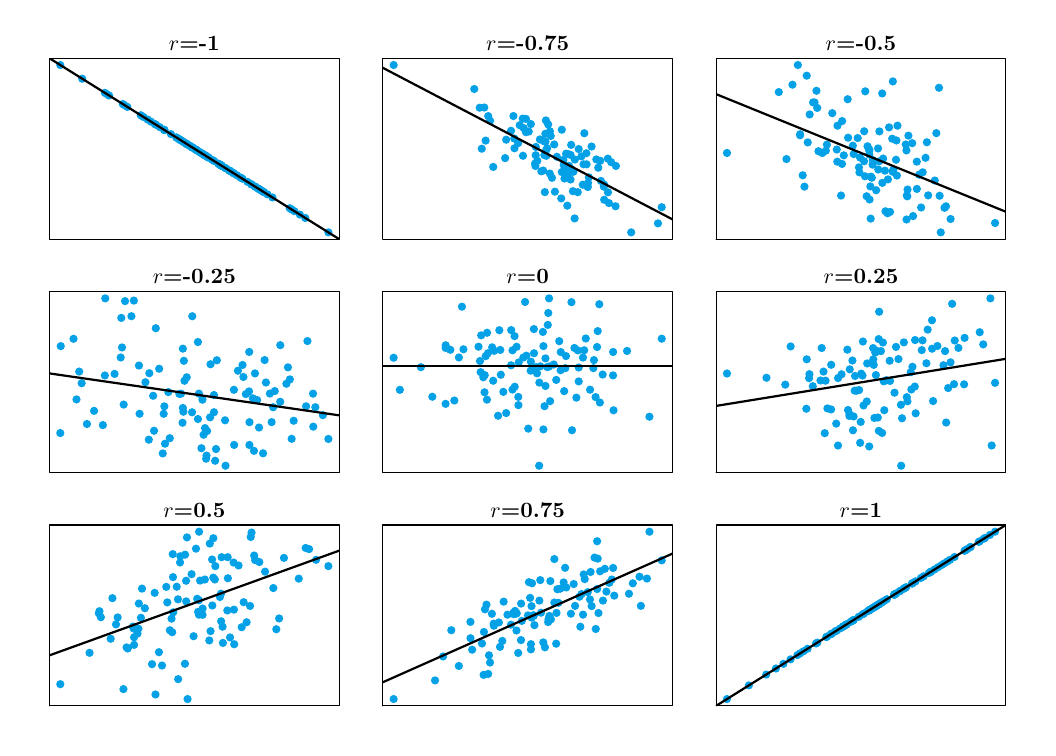
\begin{tikzpicture}[x=1pt,y=1pt]
\definecolor{fillColor}{RGB}{255,255,255}
\path[use as bounding box,fill=fillColor,fill opacity=0.00] (0,0) rectangle (361.35,252.94);
\begin{scope}
\path[clip] (  7.92,176.55) rectangle (112.53,241.86);
\definecolor{fillColor}{RGB}{5,161,230}

\path[fill=fillColor] ( 34.83,225.06) circle (  1.49);

\path[fill=fillColor] ( 57.37,210.99) circle (  1.49);

\path[fill=fillColor] ( 47.72,217.01) circle (  1.49);

\path[fill=fillColor] ( 60.53,209.02) circle (  1.49);

\path[fill=fillColor] ( 68.84,203.83) circle (  1.49);

\path[fill=fillColor] ( 69.51,203.41) circle (  1.49);

\path[fill=fillColor] ( 59.64,209.57) circle (  1.49);

\path[fill=fillColor] ( 56.31,211.65) circle (  1.49);

\path[fill=fillColor] ( 46.35,217.87) circle (  1.49);

\path[fill=fillColor] ( 49.43,215.94) circle (  1.49);

\path[fill=fillColor] ( 55.63,212.07) circle (  1.49);

\path[fill=fillColor] ( 63.20,207.35) circle (  1.49);

\path[fill=fillColor] ( 70.11,203.03) circle (  1.49);

\path[fill=fillColor] ( 63.40,207.22) circle (  1.49);

\path[fill=fillColor] ( 57.58,210.86) circle (  1.49);

\path[fill=fillColor] ( 28.57,228.97) circle (  1.49);

\path[fill=fillColor] ( 95.36,187.27) circle (  1.49);

\path[fill=fillColor] ( 71.32,202.28) circle (  1.49);

\path[fill=fillColor] ( 54.58,212.73) circle (  1.49);

\path[fill=fillColor] ( 58.68,210.17) circle (  1.49);

\path[fill=fillColor] ( 64.07,206.80) circle (  1.49);

\path[fill=fillColor] ( 96.35,186.65) circle (  1.49);

\path[fill=fillColor] ( 45.95,218.12) circle (  1.49);

\path[fill=fillColor] ( 29.44,228.42) circle (  1.49);

\path[fill=fillColor] ( 69.90,203.16) circle (  1.49);

\path[fill=fillColor] ( 63.45,207.19) circle (  1.49);

\path[fill=fillColor] ( 57.14,211.13) circle (  1.49);

\path[fill=fillColor] ( 65.11,206.15) circle (  1.49);

\path[fill=fillColor] ( 53.67,213.30) circle (  1.49);

\path[fill=fillColor] ( 57.52,210.89) circle (  1.49);

\path[fill=fillColor] ( 65.40,205.97) circle (  1.49);

\path[fill=fillColor] ( 61.18,208.61) circle (  1.49);

\path[fill=fillColor] ( 58.49,210.29) circle (  1.49);

\path[fill=fillColor] ( 44.58,218.97) circle (  1.49);

\path[fill=fillColor] ( 27.90,229.39) circle (  1.49);

\path[fill=fillColor] ( 85.37,193.50) circle (  1.49);

\path[fill=fillColor] ( 83.86,194.45) circle (  1.49);

\path[fill=fillColor] ( 59.50,209.65) circle (  1.49);

\path[fill=fillColor] ( 55.34,212.25) circle (  1.49);

\path[fill=fillColor] ( 88.44,191.59) circle (  1.49);

\path[fill=fillColor] ( 75.54,199.64) circle (  1.49);

\path[fill=fillColor] ( 72.90,201.29) circle (  1.49);

\path[fill=fillColor] ( 62.28,207.92) circle (  1.49);

\path[fill=fillColor] ( 62.15,208.00) circle (  1.49);

\path[fill=fillColor] ( 40.86,221.29) circle (  1.49);

\path[fill=fillColor] ( 77.09,198.68) circle (  1.49);

\path[fill=fillColor] ( 57.64,210.81) circle (  1.49);

\path[fill=fillColor] ( 73.60,200.86) circle (  1.49);

\path[fill=fillColor] ( 64.40,206.60) circle (  1.49);

\path[fill=fillColor] ( 19.71,234.49) circle (  1.49);

\path[fill=fillColor] ( 62.68,207.67) circle (  1.49);

\path[fill=fillColor] ( 80.77,196.38) circle (  1.49);

\path[fill=fillColor] ( 60.71,208.90) circle (  1.49);

\path[fill=fillColor] ( 74.29,200.42) circle (  1.49);

\path[fill=fillColor] ( 76.85,198.82) circle (  1.49);

\path[fill=fillColor] ( 41.84,220.68) circle (  1.49);

\path[fill=fillColor] ( 56.42,211.58) circle (  1.49);

\path[fill=fillColor] ( 94.68,187.69) circle (  1.49);

\path[fill=fillColor] ( 74.46,200.32) circle (  1.49);

\path[fill=fillColor] ( 49.25,216.06) circle (  1.49);

\path[fill=fillColor] ( 54.81,212.59) circle (  1.49);

\path[fill=fillColor] ( 63.92,206.89) circle (  1.49);

\path[fill=fillColor] ( 83.44,194.71) circle (  1.49);

\path[fill=fillColor] ( 64.34,206.63) circle (  1.49);

\path[fill=fillColor] ( 53.90,213.15) circle (  1.49);

\path[fill=fillColor] ( 69.22,203.59) circle (  1.49);

\path[fill=fillColor] ( 80.89,196.31) circle (  1.49);

\path[fill=fillColor] ( 57.29,211.03) circle (  1.49);

\path[fill=fillColor] ( 83.19,194.87) circle (  1.49);

\path[fill=fillColor] ( 77.65,198.33) circle (  1.49);

\path[fill=fillColor] ( 73.07,201.18) circle (  1.49);

\path[fill=fillColor] ( 86.67,192.70) circle (  1.49);

\path[fill=fillColor] ( 66.77,205.11) circle (  1.49);

\path[fill=fillColor] ( 51.75,214.49) circle (  1.49);

\path[fill=fillColor] ( 61.09,208.66) circle (  1.49);

\path[fill=fillColor] ( 36.02,224.31) circle (  1.49);

\path[fill=fillColor] ( 98.35,185.40) circle (  1.49);

\path[fill=fillColor] ( 59.45,209.69) circle (  1.49);

\path[fill=fillColor] ( 11.79,239.44) circle (  1.49);

\path[fill=fillColor] ( 34.38,225.34) circle (  1.49);

\path[fill=fillColor] ( 79.44,197.21) circle (  1.49);

\path[fill=fillColor] ( 65.23,206.08) circle (  1.49);

\path[fill=fillColor] ( 69.73,203.27) circle (  1.49);

\path[fill=fillColor] ( 43.38,219.72) circle (  1.49);

\path[fill=fillColor] (108.66,178.97) circle (  1.49);

\path[fill=fillColor] ( 49.38,215.98) circle (  1.49);

\path[fill=fillColor] ( 70.16,203.00) circle (  1.49);

\path[fill=fillColor] ( 85.12,193.66) circle (  1.49);

\path[fill=fillColor] (100.31,184.18) circle (  1.49);

\path[fill=fillColor] ( 59.36,209.74) circle (  1.49);

\path[fill=fillColor] ( 84.57,194.00) circle (  1.49);

\path[fill=fillColor] ( 71.71,202.03) circle (  1.49);

\path[fill=fillColor] ( 82.23,195.47) circle (  1.49);

\path[fill=fillColor] ( 82.12,195.53) circle (  1.49);

\path[fill=fillColor] ( 70.13,203.02) circle (  1.49);

\path[fill=fillColor] ( 73.04,201.20) circle (  1.49);

\path[fill=fillColor] ( 55.07,212.42) circle (  1.49);

\path[fill=fillColor] ( 83.92,194.41) circle (  1.49);

\path[fill=fillColor] ( 69.38,203.49) circle (  1.49);

\path[fill=fillColor] ( 67.35,204.76) circle (  1.49);
\end{scope}
\begin{scope}
\path[clip] (  0.00,168.63) rectangle (120.45,252.94);
\definecolor{drawColor}{RGB}{0,0,0}

\node[text=drawColor,anchor=base,inner sep=0pt, outer sep=0pt, scale=  0.79] at ( 60.22,244.63) {\bfseries $r$=-1};

\node[text=drawColor,anchor=base,inner sep=0pt, outer sep=0pt, scale=  0.66] at ( 60.22,146.45) {$X$};
\end{scope}
\begin{scope}
\path[clip] (  7.92,176.55) rectangle (112.53,241.86);
\definecolor{drawColor}{RGB}{0,0,0}

\path[draw=drawColor,line width= 0.8pt,line join=round,line cap=round] (  7.92,241.86) -- (112.53,176.55);
\end{scope}
\begin{scope}
\path[clip] (  0.00,  0.00) rectangle (361.35,252.94);
\definecolor{drawColor}{RGB}{0,0,0}

\path[draw=drawColor,line width= 0.4pt,line join=round,line cap=round] (  7.92,176.55) --
	(112.53,176.55) --
	(112.53,241.86) --
	(  7.92,241.86) --
	(  7.92,176.55);
\end{scope}
\begin{scope}
\path[clip] (128.37,176.55) rectangle (232.98,241.86);
\definecolor{fillColor}{RGB}{5,161,230}

\path[fill=fillColor] (196.17,198.07) circle (  1.49);

\path[fill=fillColor] (208.32,190.76) circle (  1.49);

\path[fill=fillColor] (183.57,206.85) circle (  1.49);

\path[fill=fillColor] (174.65,215.66) circle (  1.49);

\path[fill=fillColor] (218.08,178.97) circle (  1.49);

\path[fill=fillColor] (167.10,219.28) circle (  1.49);

\path[fill=fillColor] (199.11,209.08) circle (  1.49);

\path[fill=fillColor] (201.96,203.56) circle (  1.49);

\path[fill=fillColor] (186.70,206.91) circle (  1.49);

\path[fill=fillColor] (201.89,207.56) circle (  1.49);

\path[fill=fillColor] (181.84,218.10) circle (  1.49);

\path[fill=fillColor] (205.48,205.33) circle (  1.49);

\path[fill=fillColor] (206.88,204.83) circle (  1.49);

\path[fill=fillColor] (172.91,212.46) circle (  1.49);

\path[fill=fillColor] (178.88,220.07) circle (  1.49);

\path[fill=fillColor] (198.77,193.50) circle (  1.49);

\path[fill=fillColor] (192.80,191.23) circle (  1.49);

\path[fill=fillColor] (187.06,214.58) circle (  1.49);

\path[fill=fillColor] (172.53,205.80) circle (  1.49);

\path[fill=fillColor] (187.33,208.67) circle (  1.49);

\path[fill=fillColor] (227.76,182.22) circle (  1.49);

\path[fill=fillColor] (161.38,230.78) circle (  1.49);

\path[fill=fillColor] (188.69,200.21) circle (  1.49);

\path[fill=fillColor] (208.18,195.48) circle (  1.49);

\path[fill=fillColor] (183.64,209.83) circle (  1.49);

\path[fill=fillColor] (165.48,212.13) circle (  1.49);

\path[fill=fillColor] (189.46,198.68) circle (  1.49);

\path[fill=fillColor] (132.24,239.44) circle (  1.49);

\path[fill=fillColor] (178.97,206.65) circle (  1.49);

\path[fill=fillColor] (175.84,212.87) circle (  1.49);

\path[fill=fillColor] (191.24,206.28) circle (  1.49);

\path[fill=fillColor] (196.18,206.97) circle (  1.49);

\path[fill=fillColor] (179.24,216.66) circle (  1.49);

\path[fill=fillColor] (183.32,203.80) circle (  1.49);

\path[fill=fillColor] (187.11,211.75) circle (  1.49);

\path[fill=fillColor] (181.07,215.41) circle (  1.49);

\path[fill=fillColor] (190.51,193.68) circle (  1.49);

\path[fill=fillColor] (186.87,193.51) circle (  1.49);

\path[fill=fillColor] (210.04,189.55) circle (  1.49);

\path[fill=fillColor] (208.29,196.24) circle (  1.49);

\path[fill=fillColor] (212.56,202.97) circle (  1.49);

\path[fill=fillColor] (195.16,199.85) circle (  1.49);

\path[fill=fillColor] (202.28,195.68) circle (  1.49);

\path[fill=fillColor] (193.58,205.14) circle (  1.49);

\path[fill=fillColor] (185.59,201.05) circle (  1.49);

\path[fill=fillColor] (186.43,211.94) circle (  1.49);

\path[fill=fillColor] (194.99,188.62) circle (  1.49);

\path[fill=fillColor] (175.90,209.36) circle (  1.49);

\path[fill=fillColor] (180.04,215.18) circle (  1.49);

\path[fill=fillColor] (210.84,204.34) circle (  1.49);

\path[fill=fillColor] (187.26,219.42) circle (  1.49);

\path[fill=fillColor] (206.18,202.33) circle (  1.49);

\path[fill=fillColor] (193.70,203.27) circle (  1.49);

\path[fill=fillColor] (202.49,196.82) circle (  1.49);

\path[fill=fillColor] (193.98,198.43) circle (  1.49);

\path[fill=fillColor] (168.23,202.62) circle (  1.49);

\path[fill=fillColor] (188.71,215.51) circle (  1.49);

\path[fill=fillColor] (196.39,210.60) circle (  1.49);

\path[fill=fillColor] (190.27,210.74) circle (  1.49);

\path[fill=fillColor] (200.86,203.57) circle (  1.49);

\path[fill=fillColor] (183.48,202.96) circle (  1.49);

\path[fill=fillColor] (195.27,207.26) circle (  1.49);

\path[fill=fillColor] (163.34,224.02) circle (  1.49);

\path[fill=fillColor] (207.15,197.57) circle (  1.49);

\path[fill=fillColor] (193.01,200.76) circle (  1.49);

\path[fill=fillColor] (196.41,201.81) circle (  1.49);

\path[fill=fillColor] (185.09,212.55) circle (  1.49);

\path[fill=fillColor] (202.77,198.85) circle (  1.49);

\path[fill=fillColor] (175.52,221.01) circle (  1.49);

\path[fill=fillColor] (195.62,203.01) circle (  1.49);

\path[fill=fillColor] (177.80,217.70) circle (  1.49);

\path[fill=fillColor] (202.39,195.35) circle (  1.49);

\path[fill=fillColor] (187.42,206.64) circle (  1.49);

\path[fill=fillColor] (197.02,193.85) circle (  1.49);

\path[fill=fillColor] (180.05,219.97) circle (  1.49);

\path[fill=fillColor] (166.41,220.98) circle (  1.49);

\path[fill=fillColor] (200.08,206.43) circle (  1.49);

\path[fill=fillColor] (197.71,205.28) circle (  1.49);

\path[fill=fillColor] (212.43,188.41) circle (  1.49);

\path[fill=fillColor] (165.00,224.09) circle (  1.49);

\path[fill=fillColor] (187.71,209.37) circle (  1.49);

\path[fill=fillColor] (193.00,216.06) circle (  1.49);

\path[fill=fillColor] (209.65,205.62) circle (  1.49);

\path[fill=fillColor] (186.29,201.29) circle (  1.49);

\path[fill=fillColor] (197.64,184.01) circle (  1.49);

\path[fill=fillColor] (200.58,196.19) circle (  1.49);

\path[fill=fillColor] (189.00,213.81) circle (  1.49);

\path[fill=fillColor] (193.84,201.35) circle (  1.49);

\path[fill=fillColor] (195.45,200.56) circle (  1.49);

\path[fill=fillColor] (209.69,193.45) circle (  1.49);

\path[fill=fillColor] (188.08,217.99) circle (  1.49);

\path[fill=fillColor] (194.53,207.39) circle (  1.49);

\path[fill=fillColor] (229.11,188.07) circle (  1.49);

\path[fill=fillColor] (164.08,209.20) circle (  1.49);

\path[fill=fillColor] (184.16,204.83) circle (  1.49);

\path[fill=fillColor] (201.14,214.79) circle (  1.49);

\path[fill=fillColor] (203.76,209.99) circle (  1.49);

\path[fill=fillColor] (197.20,200.87) circle (  1.49);

\path[fill=fillColor] (177.25,211.24) circle (  1.49);

\path[fill=fillColor] (196.25,200.79) circle (  1.49);
\end{scope}
\begin{scope}
\path[clip] (120.45,168.63) rectangle (240.90,252.94);
\definecolor{drawColor}{RGB}{0,0,0}

\node[text=drawColor,anchor=base,inner sep=0pt, outer sep=0pt, scale=  0.79] at (180.68,244.63) {\bfseries $r$=-0.75};

\node[text=drawColor,anchor=base,inner sep=0pt, outer sep=0pt, scale=  0.66] at (180.68,146.45) {$X$};

\node[text=drawColor,rotate= 90.00,anchor=base,inner sep=0pt, outer sep=0pt, scale=  0.66] at (103.03,209.20) {$Y$};
\end{scope}
\begin{scope}
\path[clip] (128.37,176.55) rectangle (232.98,241.86);
\definecolor{drawColor}{RGB}{0,0,0}

\path[draw=drawColor,line width= 0.8pt,line join=round,line cap=round] (128.37,238.41) -- (232.98,183.67);
\end{scope}
\begin{scope}
\path[clip] (  0.00,  0.00) rectangle (361.35,252.94);
\definecolor{drawColor}{RGB}{0,0,0}

\path[draw=drawColor,line width= 0.4pt,line join=round,line cap=round] (128.37,176.55) --
	(232.98,176.55) --
	(232.98,241.86) --
	(128.37,241.86) --
	(128.37,176.55);
\end{scope}
\begin{scope}
\path[clip] (248.82,176.55) rectangle (353.43,241.86);
\definecolor{fillColor}{RGB}{5,161,230}

\path[fill=fillColor] (299.93,213.05) circle (  1.49);

\path[fill=fillColor] (324.45,205.91) circle (  1.49);

\path[fill=fillColor] (298.48,207.26) circle (  1.49);

\path[fill=fillColor] (284.35,225.91) circle (  1.49);

\path[fill=fillColor] (324.92,211.53) circle (  1.49);

\path[fill=fillColor] (252.69,207.66) circle (  1.49);

\path[fill=fillColor] (305.39,205.08) circle (  1.49);

\path[fill=fillColor] (303.15,192.02) circle (  1.49);

\path[fill=fillColor] (312.83,201.68) circle (  1.49);

\path[fill=fillColor] (329.94,178.97) circle (  1.49);

\path[fill=fillColor] (309.12,205.64) circle (  1.49);

\path[fill=fillColor] (292.55,204.51) circle (  1.49);

\path[fill=fillColor] (294.27,203.70) circle (  1.49);

\path[fill=fillColor] (288.80,210.69) circle (  1.49);

\path[fill=fillColor] (296.46,213.17) circle (  1.49);

\path[fill=fillColor] (304.07,209.01) circle (  1.49);

\path[fill=fillColor] (313.78,205.21) circle (  1.49);

\path[fill=fillColor] (281.87,211.48) circle (  1.49);

\path[fill=fillColor] (300.79,205.99) circle (  1.49);

\path[fill=fillColor] (311.62,186.36) circle (  1.49);

\path[fill=fillColor] (302.57,199.24) circle (  1.49);

\path[fill=fillColor] (313.91,212.18) circle (  1.49);

\path[fill=fillColor] (309.97,186.59) circle (  1.49);

\path[fill=fillColor] (285.30,223.94) circle (  1.49);

\path[fill=fillColor] (285.03,230.13) circle (  1.49);

\path[fill=fillColor] (302.66,229.93) circle (  1.49);

\path[fill=fillColor] (305.03,198.72) circle (  1.49);

\path[fill=fillColor] (302.27,215.50) circle (  1.49);

\path[fill=fillColor] (333.49,183.80) circle (  1.49);

\path[fill=fillColor] (304.23,190.85) circle (  1.49);

\path[fill=fillColor] (314.30,217.53) circle (  1.49);

\path[fill=fillColor] (298.17,210.28) circle (  1.49);

\path[fill=fillColor] (312.51,200.90) circle (  1.49);

\path[fill=fillColor] (309.76,201.27) circle (  1.49);

\path[fill=fillColor] (294.90,206.80) circle (  1.49);

\path[fill=fillColor] (318.25,213.92) circle (  1.49);

\path[fill=fillColor] (308.78,229.17) circle (  1.49);

\path[fill=fillColor] (310.87,198.12) circle (  1.49);

\path[fill=fillColor] (319.93,184.86) circle (  1.49);

\path[fill=fillColor] (304.50,195.58) circle (  1.49);

\path[fill=fillColor] (331.82,188.39) circle (  1.49);

\path[fill=fillColor] (329.53,192.20) circle (  1.49);

\path[fill=fillColor] (290.75,222.04) circle (  1.49);

\path[fill=fillColor] (307.34,201.69) circle (  1.49);

\path[fill=fillColor] (307.76,215.46) circle (  1.49);

\path[fill=fillColor] (305.31,203.44) circle (  1.49);

\path[fill=fillColor] (317.58,183.62) circle (  1.49);

\path[fill=fillColor] (323.40,200.67) circle (  1.49);

\path[fill=fillColor] (329.30,231.22) circle (  1.49);

\path[fill=fillColor] (300.38,202.46) circle (  1.49);

\path[fill=fillColor] (303.48,210.07) circle (  1.49);

\path[fill=fillColor] (276.36,232.34) circle (  1.49);

\path[fill=fillColor] (285.75,208.29) circle (  1.49);

\path[fill=fillColor] (306.60,194.20) circle (  1.49);

\path[fill=fillColor] (317.55,208.59) circle (  1.49);

\path[fill=fillColor] (319.62,211.19) circle (  1.49);

\path[fill=fillColor] (304.11,208.50) circle (  1.49);

\path[fill=fillColor] (317.29,210.73) circle (  1.49);

\path[fill=fillColor] (317.69,192.36) circle (  1.49);

\path[fill=fillColor] (328.34,214.82) circle (  1.49);

\path[fill=fillColor] (302.22,204.67) circle (  1.49);

\path[fill=fillColor] (279.12,214.43) circle (  1.49);

\path[fill=fillColor] (321.29,204.53) circle (  1.49);

\path[fill=fillColor] (283.79,225.92) circle (  1.49);

\path[fill=fillColor] (304.70,199.10) circle (  1.49);

\path[fill=fillColor] (325.39,192.34) circle (  1.49);

\path[fill=fillColor] (288.42,208.50) circle (  1.49);

\path[fill=fillColor] (281.51,235.59) circle (  1.49);

\path[fill=fillColor] (307.28,209.29) circle (  1.49);

\path[fill=fillColor] (322.84,187.96) circle (  1.49);

\path[fill=fillColor] (274.19,205.45) circle (  1.49);

\path[fill=fillColor] (312.63,233.51) circle (  1.49);

\path[fill=fillColor] (279.10,214.07) circle (  1.49);

\path[fill=fillColor] (310.70,185.88) circle (  1.49);

\path[fill=fillColor] (293.91,192.28) circle (  1.49);

\path[fill=fillColor] (317.86,192.00) circle (  1.49);

\path[fill=fillColor] (317.94,194.44) circle (  1.49);

\path[fill=fillColor] (321.31,194.67) circle (  1.49);

\path[fill=fillColor] (308.83,196.85) circle (  1.49);

\path[fill=fillColor] (296.31,227.08) circle (  1.49);

\path[fill=fillColor] (294.31,219.19) circle (  1.49);

\path[fill=fillColor] (300.56,200.65) circle (  1.49);

\path[fill=fillColor] (287.14,207.63) circle (  1.49);

\path[fill=fillColor] (280.68,195.50) circle (  1.49);

\path[fill=fillColor] (292.62,217.51) circle (  1.49);

\path[fill=fillColor] (278.30,239.44) circle (  1.49);

\path[fill=fillColor] (322.14,199.82) circle (  1.49);

\path[fill=fillColor] (282.57,221.59) circle (  1.49);

\path[fill=fillColor] (304.12,207.11) circle (  1.49);

\path[fill=fillColor] (331.29,187.84) circle (  1.49);

\path[fill=fillColor] (304.62,183.94) circle (  1.49);

\path[fill=fillColor] (314.09,199.50) circle (  1.49);

\path[fill=fillColor] (311.26,216.91) circle (  1.49);

\path[fill=fillColor] (349.56,182.35) circle (  1.49);

\path[fill=fillColor] (292.37,208.91) circle (  1.49);

\path[fill=fillColor] (307.71,204.66) circle (  1.49);

\path[fill=fillColor] (280.05,199.60) circle (  1.49);

\path[fill=fillColor] (271.41,229.66) circle (  1.49);

\path[fill=fillColor] (327.78,197.70) circle (  1.49);

\path[fill=fillColor] (312.39,212.82) circle (  1.49);
\end{scope}
\begin{scope}
\path[clip] (240.90,168.63) rectangle (361.35,252.94);
\definecolor{drawColor}{RGB}{0,0,0}

\node[text=drawColor,anchor=base,inner sep=0pt, outer sep=0pt, scale=  0.79] at (301.12,244.63) {\bfseries $r$=-0.5};

\node[text=drawColor,anchor=base,inner sep=0pt, outer sep=0pt, scale=  0.66] at (301.12,146.45) {$X$};

\node[text=drawColor,rotate= 90.00,anchor=base,inner sep=0pt, outer sep=0pt, scale=  0.66] at (223.48,209.20) {$Y$};
\end{scope}
\begin{scope}
\path[clip] (248.82,176.55) rectangle (353.43,241.86);
\definecolor{drawColor}{RGB}{0,0,0}

\path[draw=drawColor,line width= 0.8pt,line join=round,line cap=round] (248.82,228.90) -- (353.43,186.43);
\end{scope}
\begin{scope}
\path[clip] (  0.00,  0.00) rectangle (361.35,252.94);
\definecolor{drawColor}{RGB}{0,0,0}

\path[draw=drawColor,line width= 0.4pt,line join=round,line cap=round] (248.82,176.55) --
	(353.43,176.55) --
	(353.43,241.86) --
	(248.82,241.86) --
	(248.82,176.55);
\end{scope}
\begin{scope}
\path[clip] (  7.92, 92.23) rectangle (112.53,157.54);
\definecolor{fillColor}{RGB}{5,161,230}

\path[fill=fillColor] ( 88.70,115.78) circle (  1.49);

\path[fill=fillColor] ( 28.04,155.12) circle (  1.49);

\path[fill=fillColor] ( 71.33,111.06) circle (  1.49);

\path[fill=fillColor] ( 56.07,136.96) circle (  1.49);

\path[fill=fillColor] ( 64.83,107.20) circle (  1.49);

\path[fill=fillColor] ( 16.57,140.51) circle (  1.49);

\path[fill=fillColor] ( 65.91,112.12) circle (  1.49);

\path[fill=fillColor] ( 43.77,104.06) circle (  1.49);

\path[fill=fillColor] ( 74.61,102.16) circle (  1.49);

\path[fill=fillColor] ( 83.60,108.45) circle (  1.49);

\path[fill=fillColor] (103.12,120.69) circle (  1.49);

\path[fill=fillColor] ( 49.39,116.10) circle (  1.49);

\path[fill=fillColor] ( 77.63,131.06) circle (  1.49);

\path[fill=fillColor] ( 63.57,105.84) circle (  1.49);

\path[fill=fillColor] ( 55.96,110.18) circle (  1.49);

\path[fill=fillColor] ( 71.50, 94.65) circle (  1.49);

\path[fill=fillColor] (101.09,139.70) circle (  1.49);

\path[fill=fillColor] ( 75.97,128.98) circle (  1.49);

\path[fill=fillColor] ( 94.05,130.20) circle (  1.49);

\path[fill=fillColor] ( 19.50,124.46) circle (  1.49);

\path[fill=fillColor] ( 68.05,100.67) circle (  1.49);

\path[fill=fillColor] ( 61.88,120.70) circle (  1.49);

\path[fill=fillColor] ( 43.96,128.07) circle (  1.49);

\path[fill=fillColor] ( 62.78,100.97) circle (  1.49);

\path[fill=fillColor] ( 21.42,109.73) circle (  1.49);

\path[fill=fillColor] ( 47.52,129.69) circle (  1.49);

\path[fill=fillColor] (103.20,108.77) circle (  1.49);

\path[fill=fillColor] ( 96.12,110.90) circle (  1.49);

\path[fill=fillColor] ( 49.63,102.61) circle (  1.49);

\path[fill=fillColor] ( 50.82,121.26) circle (  1.49);

\path[fill=fillColor] (106.67,112.92) circle (  1.49);

\path[fill=fillColor] ( 31.41,127.83) circle (  1.49);

\path[fill=fillColor] ( 67.32,113.97) circle (  1.49);

\path[fill=fillColor] ( 51.35,104.59) circle (  1.49);

\path[fill=fillColor] (100.60,116.12) circle (  1.49);

\path[fill=fillColor] ( 94.74,125.85) circle (  1.49);

\path[fill=fillColor] ( 57.48,126.61) circle (  1.49);

\path[fill=fillColor] ( 64.48, 97.18) circle (  1.49);

\path[fill=fillColor] ( 66.06,131.31) circle (  1.49);

\path[fill=fillColor] ( 80.12,102.15) circle (  1.49);

\path[fill=fillColor] ( 56.26,114.17) circle (  1.49);

\path[fill=fillColor] ( 81.76,100.03) circle (  1.49);

\path[fill=fillColor] ( 86.09,124.72) circle (  1.49);

\path[fill=fillColor] ( 82.13,128.01) circle (  1.49);

\path[fill=fillColor] ( 81.38,119.00) circle (  1.49);

\path[fill=fillColor] ( 91.26,117.75) circle (  1.49);

\path[fill=fillColor] ( 33.83,148.07) circle (  1.49);

\path[fill=fillColor] ( 37.49,148.67) circle (  1.49);

\path[fill=fillColor] ( 35.18,154.13) circle (  1.49);

\path[fill=fillColor] ( 88.15,110.40) circle (  1.49);

\path[fill=fillColor] ( 89.27,121.62) circle (  1.49);

\path[fill=fillColor] ( 34.09,137.39) circle (  1.49);

\path[fill=fillColor] ( 48.81, 99.09) circle (  1.49);

\path[fill=fillColor] ( 59.48,148.66) circle (  1.49);

\path[fill=fillColor] ( 80.06,135.77) circle (  1.49);

\path[fill=fillColor] ( 85.05, 99.14) circle (  1.49);

\path[fill=fillColor] ( 45.34,119.93) circle (  1.49);

\path[fill=fillColor] ( 18.62,128.67) circle (  1.49);

\path[fill=fillColor] ( 79.99,121.51) circle (  1.49);

\path[fill=fillColor] ( 40.21,130.85) circle (  1.49);

\path[fill=fillColor] (108.66,104.32) circle (  1.49);

\path[fill=fillColor] ( 45.67,107.28) circle (  1.49);

\path[fill=fillColor] ( 64.08,108.25) circle (  1.49);

\path[fill=fillColor] ( 11.79,106.46) circle (  1.49);

\path[fill=fillColor] ( 55.42,120.68) circle (  1.49);

\path[fill=fillColor] ( 87.52,120.72) circle (  1.49);

\path[fill=fillColor] ( 61.53,111.53) circle (  1.49);

\path[fill=fillColor] ( 46.30,144.34) circle (  1.49);

\path[fill=fillColor] ( 27.89,127.26) circle (  1.49);

\path[fill=fillColor] ( 23.99,114.47) circle (  1.49);

\path[fill=fillColor] ( 56.07,115.52) circle (  1.49);

\path[fill=fillColor] ( 56.44,132.56) circle (  1.49);

\path[fill=fillColor] ( 63.15,118.51) circle (  1.49);

\path[fill=fillColor] ( 61.52,139.34) circle (  1.49);

\path[fill=fillColor] ( 17.64,118.62) circle (  1.49);

\path[fill=fillColor] ( 38.36,154.32) circle (  1.49);

\path[fill=fillColor] ( 54.81,120.60) circle (  1.49);

\path[fill=fillColor] ( 42.55,124.82) circle (  1.49);

\path[fill=fillColor] ( 27.17,109.33) circle (  1.49);

\path[fill=fillColor] ( 77.96,126.73) circle (  1.49);

\path[fill=fillColor] ( 59.40,113.96) circle (  1.49);

\path[fill=fillColor] ( 74.53,122.08) circle (  1.49);

\path[fill=fillColor] ( 78.83,120.53) circle (  1.49);

\path[fill=fillColor] ( 56.66,125.35) circle (  1.49);

\path[fill=fillColor] ( 82.92,118.37) circle (  1.49);

\path[fill=fillColor] ( 95.38,104.37) circle (  1.49);

\path[fill=fillColor] ( 85.62,132.83) circle (  1.49);

\path[fill=fillColor] ( 64.63, 98.32) circle (  1.49);

\path[fill=fillColor] ( 49.15,113.40) circle (  1.49);

\path[fill=fillColor] ( 67.32,120.19) circle (  1.49);

\path[fill=fillColor] ( 33.61,133.76) circle (  1.49);

\path[fill=fillColor] ( 11.95,137.86) circle (  1.49);

\path[fill=fillColor] ( 34.69,116.75) circle (  1.49);

\path[fill=fillColor] ( 80.16,110.38) circle (  1.49);

\path[fill=fillColor] ( 93.49,124.27) circle (  1.49);

\path[fill=fillColor] ( 67.74, 96.45) circle (  1.49);

\path[fill=fillColor] ( 68.35,132.75) circle (  1.49);

\path[fill=fillColor] ( 40.44,113.43) circle (  1.49);

\path[fill=fillColor] (103.94,115.79) circle (  1.49);

\path[fill=fillColor] ( 91.28,138.21) circle (  1.49);
\end{scope}
\begin{scope}
\path[clip] (  0.00, 84.31) rectangle (120.45,168.63);
\definecolor{drawColor}{RGB}{0,0,0}

\node[text=drawColor,anchor=base,inner sep=0pt, outer sep=0pt, scale=  0.79] at ( 60.22,160.32) {\bfseries $r$=-0.25};

\node[text=drawColor,anchor=base,inner sep=0pt, outer sep=0pt, scale=  0.66] at ( 60.22, 62.14) {$X$};
\end{scope}
\begin{scope}
\path[clip] (  7.92, 92.23) rectangle (112.53,157.54);
\definecolor{drawColor}{RGB}{0,0,0}

\path[draw=drawColor,line width= 0.8pt,line join=round,line cap=round] (  7.92,128.00) -- (112.53,112.86);
\end{scope}
\begin{scope}
\path[clip] (  0.00,  0.00) rectangle (361.35,252.94);
\definecolor{drawColor}{RGB}{0,0,0}

\path[draw=drawColor,line width= 0.4pt,line join=round,line cap=round] (  7.92, 92.23) --
	(112.53, 92.23) --
	(112.53,157.54) --
	(  7.92,157.54) --
	(  7.92, 92.23);
\end{scope}
\begin{scope}
\path[clip] (128.37, 92.23) rectangle (232.98,157.54);
\definecolor{fillColor}{RGB}{5,161,230}

\path[fill=fillColor] (180.21,134.42) circle (  1.49);

\path[fill=fillColor] (196.70,107.47) circle (  1.49);

\path[fill=fillColor] (174.72,143.66) circle (  1.49);

\path[fill=fillColor] (186.37,137.87) circle (  1.49);

\path[fill=fillColor] (187.10,133.43) circle (  1.49);

\path[fill=fillColor] (199.11,125.12) circle (  1.49);

\path[fill=fillColor] (175.94,141.47) circle (  1.49);

\path[fill=fillColor] (164.63,126.62) circle (  1.49);

\path[fill=fillColor] (168.22,125.35) circle (  1.49);

\path[fill=fillColor] (132.24,133.67) circle (  1.49);

\path[fill=fillColor] (179.73,153.82) circle (  1.49);

\path[fill=fillColor] (163.87,141.76) circle (  1.49);

\path[fill=fillColor] (211.54,135.75) circle (  1.49);

\path[fill=fillColor] (151.02,117.01) circle (  1.49);

\path[fill=fillColor] (186.36,107.77) circle (  1.49);

\path[fill=fillColor] (181.75,128.99) circle (  1.49);

\path[fill=fillColor] (179.10,133.74) circle (  1.49);

\path[fill=fillColor] (162.91,137.65) circle (  1.49);

\path[fill=fillColor] (198.27,119.25) circle (  1.49);

\path[fill=fillColor] (157.46,136.73) circle (  1.49);

\path[fill=fillColor] (188.12,149.84) circle (  1.49);

\path[fill=fillColor] (204.41,129.91) circle (  1.49);

\path[fill=fillColor] (176.66,137.63) circle (  1.49);

\path[fill=fillColor] (197.58,137.20) circle (  1.49);

\path[fill=fillColor] (196.50,153.75) circle (  1.49);

\path[fill=fillColor] (186.77,116.16) circle (  1.49);

\path[fill=fillColor] (151.03,137.21) circle (  1.49);

\path[fill=fillColor] (192.08,139.66) circle (  1.49);

\path[fill=fillColor] (205.98,143.30) circle (  1.49);

\path[fill=fillColor] (175.99,123.19) circle (  1.49);

\path[fill=fillColor] (165.51,134.25) circle (  1.49);

\path[fill=fillColor] (216.58,136.12) circle (  1.49);

\path[fill=fillColor] (156.92,152.12) circle (  1.49);

\path[fill=fillColor] (166.31,135.31) circle (  1.49);

\path[fill=fillColor] (151.04,138.17) circle (  1.49);

\path[fill=fillColor] (201.10,136.37) circle (  1.49);

\path[fill=fillColor] (224.67,112.36) circle (  1.49);

\path[fill=fillColor] (170.97,127.53) circle (  1.49);

\path[fill=fillColor] (175.20,136.35) circle (  1.49);

\path[fill=fillColor] (154.18,118.21) circle (  1.49);

\path[fill=fillColor] (198.79,136.32) circle (  1.49);

\path[fill=fillColor] (205.22,119.45) circle (  1.49);

\path[fill=fillColor] (229.11,140.55) circle (  1.49);

\path[fill=fillColor] (184.82, 94.65) circle (  1.49);

\path[fill=fillColor] (188.78,117.98) circle (  1.49);

\path[fill=fillColor] (169.98,112.71) circle (  1.49);

\path[fill=fillColor] (174.68,130.94) circle (  1.49);

\path[fill=fillColor] (177.28,119.52) circle (  1.49);

\path[fill=fillColor] (134.49,122.07) circle (  1.49);

\path[fill=fillColor] (168.55,136.16) circle (  1.49);

\path[fill=fillColor] (211.70,114.68) circle (  1.49);

\path[fill=fillColor] (184.89,124.68) circle (  1.49);

\path[fill=fillColor] (170.43,143.61) circle (  1.49);

\path[fill=fillColor] (188.45,130.51) circle (  1.49);

\path[fill=fillColor] (206.77,117.48) circle (  1.49);

\path[fill=fillColor] (163.68,128.46) circle (  1.49);

\path[fill=fillColor] (205.75,137.54) circle (  1.49);

\path[fill=fillColor] (182.91,144.03) circle (  1.49);

\path[fill=fillColor] (200.64,133.73) circle (  1.49);

\path[fill=fillColor] (165.08,121.19) circle (  1.49);

\path[fill=fillColor] (187.75,130.29) circle (  1.49);

\path[fill=fillColor] (186.17,142.99) circle (  1.49);

\path[fill=fillColor] (187.94,145.53) circle (  1.49);

\path[fill=fillColor] (165.96,118.53) circle (  1.49);

\path[fill=fillColor] (181.85,132.23) circle (  1.49);

\path[fill=fillColor] (185.24,130.57) circle (  1.49);

\path[fill=fillColor] (175.18,122.17) circle (  1.49);

\path[fill=fillColor] (182.96,135.29) circle (  1.49);

\path[fill=fillColor] (142.09,130.26) circle (  1.49);

\path[fill=fillColor] (165.16,127.39) circle (  1.49);

\path[fill=fillColor] (177.44,131.99) circle (  1.49);

\path[fill=fillColor] (155.82,133.77) circle (  1.49);

\path[fill=fillColor] (171.88,121.34) circle (  1.49);

\path[fill=fillColor] (146.22,119.58) circle (  1.49);

\path[fill=fillColor] (211.52,127.29) circle (  1.49);

\path[fill=fillColor] (194.29,129.91) circle (  1.49);

\path[fill=fillColor] (152.73,136.53) circle (  1.49);

\path[fill=fillColor] (177.33,116.55) circle (  1.49);

\path[fill=fillColor] (192.57,129.15) circle (  1.49);

\path[fill=fillColor] (167.84,137.43) circle (  1.49);

\path[fill=fillColor] (172.91,113.68) circle (  1.49);

\path[fill=fillColor] (201.67,140.62) circle (  1.49);

\path[fill=fillColor] (206.55,153.00) circle (  1.49);

\path[fill=fillColor] (187.11,123.47) circle (  1.49);

\path[fill=fillColor] (199.12,130.14) circle (  1.49);

\path[fill=fillColor] (188.41,155.12) circle (  1.49);

\path[fill=fillColor] (194.53,134.27) circle (  1.49);

\path[fill=fillColor] (190.09,131.23) circle (  1.49);

\path[fill=fillColor] (183.68,130.27) circle (  1.49);

\path[fill=fillColor] (193.87,121.60) circle (  1.49);

\path[fill=fillColor] (192.63,135.72) circle (  1.49);

\path[fill=fillColor] (163.44,132.47) circle (  1.49);

\path[fill=fillColor] (166.00,142.69) circle (  1.49);

\path[fill=fillColor] (191.00,125.66) circle (  1.49);

\path[fill=fillColor] (170.77,136.49) circle (  1.49);

\path[fill=fillColor] (204.62,132.82) circle (  1.49);

\path[fill=fillColor] (207.77,127.60) circle (  1.49);

\path[fill=fillColor] (180.88,108.05) circle (  1.49);

\path[fill=fillColor] (184.06,128.02) circle (  1.49);

\path[fill=fillColor] (203.21,122.12) circle (  1.49);
\end{scope}
\begin{scope}
\path[clip] (120.45, 84.31) rectangle (240.90,168.63);
\definecolor{drawColor}{RGB}{0,0,0}

\node[text=drawColor,anchor=base,inner sep=0pt, outer sep=0pt, scale=  0.79] at (180.68,160.32) {\bfseries $r$=0};

\node[text=drawColor,anchor=base,inner sep=0pt, outer sep=0pt, scale=  0.66] at (180.68, 62.14) {$X$};

\node[text=drawColor,rotate= 90.00,anchor=base,inner sep=0pt, outer sep=0pt, scale=  0.66] at (103.03,124.89) {$Y$};
\end{scope}
\begin{scope}
\path[clip] (128.37, 92.23) rectangle (232.98,157.54);
\definecolor{drawColor}{RGB}{0,0,0}

\path[draw=drawColor,line width= 0.8pt,line join=round,line cap=round] (128.37,130.66) -- (232.98,130.66);
\end{scope}
\begin{scope}
\path[clip] (  0.00,  0.00) rectangle (361.35,252.94);
\definecolor{drawColor}{RGB}{0,0,0}

\path[draw=drawColor,line width= 0.4pt,line join=round,line cap=round] (128.37, 92.23) --
	(232.98, 92.23) --
	(232.98,157.54) --
	(128.37,157.54) --
	(128.37, 92.23);
\end{scope}
\begin{scope}
\path[clip] (248.82, 92.23) rectangle (353.43,157.54);
\definecolor{fillColor}{RGB}{5,161,230}

\path[fill=fillColor] (305.71,131.09) circle (  1.49);

\path[fill=fillColor] (327.17,118.02) circle (  1.49);

\path[fill=fillColor] (344.02,142.88) circle (  1.49);

\path[fill=fillColor] (281.37,115.24) circle (  1.49);

\path[fill=fillColor] (296.19,136.58) circle (  1.49);

\path[fill=fillColor] (332.61,122.72) circle (  1.49);

\path[fill=fillColor] (345.29,138.49) circle (  1.49);

\path[fill=fillColor] (334.99,139.89) circle (  1.49);

\path[fill=fillColor] (296.92,112.64) circle (  1.49);

\path[fill=fillColor] (331.89,110.26) circle (  1.49);

\path[fill=fillColor] (316.60,139.22) circle (  1.49);

\path[fill=fillColor] (303.35,131.60) circle (  1.49);

\path[fill=fillColor] (319.31,122.20) circle (  1.49);

\path[fill=fillColor] (347.87,155.12) circle (  1.49);

\path[fill=fillColor] (334.74,124.12) circle (  1.49);

\path[fill=fillColor] (298.97,127.09) circle (  1.49);

\path[fill=fillColor] (320.66,140.06) circle (  1.49);

\path[fill=fillColor] (294.09,127.69) circle (  1.49);

\path[fill=fillColor] (296.97,113.28) circle (  1.49);

\path[fill=fillColor] (288.02,106.41) circle (  1.49);

\path[fill=fillColor] (325.21,143.83) circle (  1.49);

\path[fill=fillColor] (323.35,139.95) circle (  1.49);

\path[fill=fillColor] (315.94,111.80) circle (  1.49);

\path[fill=fillColor] (304.09,101.62) circle (  1.49);

\path[fill=fillColor] (303.21,117.87) circle (  1.49);

\path[fill=fillColor] (292.80,101.95) circle (  1.49);

\path[fill=fillColor] (331.50,136.07) circle (  1.49);

\path[fill=fillColor] (323.07,136.42) circle (  1.49);

\path[fill=fillColor] (333.47,132.00) circle (  1.49);

\path[fill=fillColor] (349.56,124.60) circle (  1.49);

\path[fill=fillColor] (286.47,125.45) circle (  1.49);

\path[fill=fillColor] (336.32,137.23) circle (  1.49);

\path[fill=fillColor] (296.42,114.78) circle (  1.49);

\path[fill=fillColor] (309.53,114.70) circle (  1.49);

\path[fill=fillColor] (288.99,115.36) circle (  1.49);

\path[fill=fillColor] (324.76,131.68) circle (  1.49);

\path[fill=fillColor] (311.61,125.29) circle (  1.49);

\path[fill=fillColor] (281.51,133.10) circle (  1.49);

\path[fill=fillColor] (292.84,126.33) circle (  1.49);

\path[fill=fillColor] (338.38,124.06) circle (  1.49);

\path[fill=fillColor] (320.56,123.26) circle (  1.49);

\path[fill=fillColor] (307.00,136.08) circle (  1.49);

\path[fill=fillColor] (319.71,130.40) circle (  1.49);

\path[fill=fillColor] (252.69,127.97) circle (  1.49);

\path[fill=fillColor] (326.78,147.21) circle (  1.49);

\path[fill=fillColor] (288.31,125.38) circle (  1.49);

\path[fill=fillColor] (286.92,137.18) circle (  1.49);

\path[fill=fillColor] (266.96,126.43) circle (  1.49);

\path[fill=fillColor] (298.22,107.46) circle (  1.49);

\path[fill=fillColor] (302.04,116.43) circle (  1.49);

\path[fill=fillColor] (305.56,133.08) circle (  1.49);

\path[fill=fillColor] (309.04,139.16) circle (  1.49);

\path[fill=fillColor] (282.49,127.73) circle (  1.49);

\path[fill=fillColor] (320.87,113.58) circle (  1.49);

\path[fill=fillColor] (306.27,135.56) circle (  1.49);

\path[fill=fillColor] (317.90,117.93) circle (  1.49);

\path[fill=fillColor] (310.28,125.55) circle (  1.49);

\path[fill=fillColor] (313.77,137.58) circle (  1.49);

\path[fill=fillColor] (299.51,121.77) circle (  1.49);

\path[fill=fillColor] (300.81,102.92) circle (  1.49);

\path[fill=fillColor] (301.21,127.92) circle (  1.49);

\path[fill=fillColor] (307.68,150.29) circle (  1.49);

\path[fill=fillColor] (330.92,130.96) circle (  1.49);

\path[fill=fillColor] (298.01,132.66) circle (  1.49);

\path[fill=fillColor] (283.69,123.38) circle (  1.49);

\path[fill=fillColor] (313.23,121.04) circle (  1.49);

\path[fill=fillColor] (308.75,106.48) circle (  1.49);

\path[fill=fillColor] (290.35,131.12) circle (  1.49);

\path[fill=fillColor] (338.55,140.84) circle (  1.49);

\path[fill=fillColor] (319.10,128.44) circle (  1.49);

\path[fill=fillColor] (311.48,132.58) circle (  1.49);

\path[fill=fillColor] (307.56,107.24) circle (  1.49);

\path[fill=fillColor] (348.34,101.96) circle (  1.49);

\path[fill=fillColor] (315.54,116.67) circle (  1.49);

\path[fill=fillColor] (292.17,109.87) circle (  1.49);

\path[fill=fillColor] (301.01,110.48) circle (  1.49);

\path[fill=fillColor] (307.50,140.41) circle (  1.49);

\path[fill=fillColor] (326.81,136.93) circle (  1.49);

\path[fill=fillColor] (273.76,123.95) circle (  1.49);

\path[fill=fillColor] (290.31,114.99) circle (  1.49);

\path[fill=fillColor] (308.33,136.07) circle (  1.49);

\path[fill=fillColor] (328.73,137.91) circle (  1.49);

\path[fill=fillColor] (307.19,112.07) circle (  1.49);

\path[fill=fillColor] (334.05,153.15) circle (  1.49);

\path[fill=fillColor] (300.43,121.98) circle (  1.49);

\path[fill=fillColor] (315.63, 94.65) circle (  1.49);

\path[fill=fillColor] (305.96,111.91) circle (  1.49);

\path[fill=fillColor] (317.67,119.42) circle (  1.49);

\path[fill=fillColor] (287.57,128.66) circle (  1.49);

\path[fill=fillColor] (298.84,121.78) circle (  1.49);

\path[fill=fillColor] (301.66,127.23) circle (  1.49);

\path[fill=fillColor] (309.34,125.15) circle (  1.49);

\path[fill=fillColor] (282.36,126.29) circle (  1.49);

\path[fill=fillColor] (301.81,139.53) circle (  1.49);

\path[fill=fillColor] (297.05,129.48) circle (  1.49);

\path[fill=fillColor] (314.66,133.18) circle (  1.49);

\path[fill=fillColor] (305.50,137.16) circle (  1.49);

\path[fill=fillColor] (275.69,137.75) circle (  1.49);

\path[fill=fillColor] (306.50,127.41) circle (  1.49);

\path[fill=fillColor] (298.45,112.45) circle (  1.49);
\end{scope}
\begin{scope}
\path[clip] (240.90, 84.31) rectangle (361.35,168.63);
\definecolor{drawColor}{RGB}{0,0,0}

\node[text=drawColor,anchor=base,inner sep=0pt, outer sep=0pt, scale=  0.79] at (301.12,160.32) {\bfseries $r$=0.25};

\node[text=drawColor,anchor=base,inner sep=0pt, outer sep=0pt, scale=  0.66] at (301.12, 62.14) {$X$};

\node[text=drawColor,rotate= 90.00,anchor=base,inner sep=0pt, outer sep=0pt, scale=  0.66] at (223.48,124.89) {$Y$};
\end{scope}
\begin{scope}
\path[clip] (248.82, 92.23) rectangle (353.43,157.54);
\definecolor{drawColor}{RGB}{0,0,0}

\path[draw=drawColor,line width= 0.8pt,line join=round,line cap=round] (248.82,116.27) -- (353.43,133.27);
\end{scope}
\begin{scope}
\path[clip] (  0.00,  0.00) rectangle (361.35,252.94);
\definecolor{drawColor}{RGB}{0,0,0}

\path[draw=drawColor,line width= 0.4pt,line join=round,line cap=round] (248.82, 92.23) --
	(353.43, 92.23) --
	(353.43,157.54) --
	(248.82,157.54) --
	(248.82, 92.23);
\end{scope}
\begin{scope}
\path[clip] (  7.92,  7.92) rectangle (112.53, 73.23);
\definecolor{fillColor}{RGB}{5,161,230}

\path[fill=fillColor] (104.21, 60.64) circle (  1.49);

\path[fill=fillColor] ( 69.47, 47.21) circle (  1.49);

\path[fill=fillColor] ( 47.43, 27.27) circle (  1.49);

\path[fill=fillColor] ( 97.95, 53.85) circle (  1.49);

\path[fill=fillColor] ( 61.58, 41.84) circle (  1.49);

\path[fill=fillColor] ( 82.20, 60.55) circle (  1.49);

\path[fill=fillColor] ( 69.90, 38.44) circle (  1.49);

\path[fill=fillColor] ( 60.82, 64.68) circle (  1.49);

\path[fill=fillColor] ( 72.34, 53.98) circle (  1.49);

\path[fill=fillColor] ( 41.31, 50.24) circle (  1.49);

\path[fill=fillColor] ( 63.21, 43.04) circle (  1.49);

\path[fill=fillColor] ( 81.84, 62.20) circle (  1.49);

\path[fill=fillColor] ( 61.94, 70.81) circle (  1.49);

\path[fill=fillColor] ( 63.20, 40.76) circle (  1.49);

\path[fill=fillColor] ( 38.44, 32.66) circle (  1.49);

\path[fill=fillColor] ( 38.04, 36.52) circle (  1.49);

\path[fill=fillColor] (101.69, 64.52) circle (  1.49);

\path[fill=fillColor] ( 59.95, 33.04) circle (  1.49);

\path[fill=fillColor] ( 52.42, 62.70) circle (  1.49);

\path[fill=fillColor] ( 66.08, 34.88) circle (  1.49);

\path[fill=fillColor] ( 34.60, 13.93) circle (  1.49);

\path[fill=fillColor] ( 72.27, 61.60) circle (  1.49);

\path[fill=fillColor] ( 22.36, 27.04) circle (  1.49);

\path[fill=fillColor] ( 88.76, 50.44) circle (  1.49);

\path[fill=fillColor] ( 50.45, 45.27) circle (  1.49);

\path[fill=fillColor] ( 90.86, 39.46) circle (  1.49);

\path[fill=fillColor] ( 35.75, 29.01) circle (  1.49);

\path[fill=fillColor] ( 62.29, 53.14) circle (  1.49);

\path[fill=fillColor] ( 53.85, 50.92) circle (  1.49);

\path[fill=fillColor] ( 67.63, 53.54) circle (  1.49);

\path[fill=fillColor] ( 74.52, 42.65) circle (  1.49);

\path[fill=fillColor] ( 25.94, 42.08) circle (  1.49);

\path[fill=fillColor] ( 65.63, 31.52) circle (  1.49);

\path[fill=fillColor] ( 66.63, 60.76) circle (  1.49);

\path[fill=fillColor] ( 57.56, 68.75) circle (  1.49);

\path[fill=fillColor] ( 70.08, 61.60) circle (  1.49);

\path[fill=fillColor] ( 74.63, 30.14) circle (  1.49);

\path[fill=fillColor] ( 80.90, 70.50) circle (  1.49);

\path[fill=fillColor] ( 51.38, 35.18) circle (  1.49);

\path[fill=fillColor] ( 64.01, 53.52) circle (  1.49);

\path[fill=fillColor] ( 52.59, 41.68) circle (  1.49);

\path[fill=fillColor] ( 30.62, 46.79) circle (  1.49);

\path[fill=fillColor] ( 52.22, 34.49) circle (  1.49);

\path[fill=fillColor] ( 57.78, 10.34) circle (  1.49);

\path[fill=fillColor] ( 69.85, 48.39) circle (  1.49);

\path[fill=fillColor] ( 74.41, 59.66) circle (  1.49);

\path[fill=fillColor] ( 76.21, 58.60) circle (  1.49);

\path[fill=fillColor] ( 55.06, 59.69) circle (  1.49);

\path[fill=fillColor] ( 77.33, 36.30) circle (  1.49);

\path[fill=fillColor] ( 66.72, 44.14) circle (  1.49);

\path[fill=fillColor] ( 85.78, 56.38) circle (  1.49);

\path[fill=fillColor] ( 46.18, 11.99) circle (  1.49);

\path[fill=fillColor] ( 57.26, 53.08) circle (  1.49);

\path[fill=fillColor] ( 40.01, 35.76) circle (  1.49);

\path[fill=fillColor] ( 89.85, 35.55) circle (  1.49);

\path[fill=fillColor] ( 83.72, 59.84) circle (  1.49);

\path[fill=fillColor] ( 61.87, 46.06) circle (  1.49);

\path[fill=fillColor] ( 51.99, 39.39) circle (  1.49);

\path[fill=fillColor] ( 45.89, 48.72) circle (  1.49);

\path[fill=fillColor] ( 38.29, 35.80) circle (  1.49);

\path[fill=fillColor] ( 32.51, 39.84) circle (  1.49);

\path[fill=fillColor] ( 57.28, 45.63) circle (  1.49);

\path[fill=fillColor] ( 31.92, 37.31) circle (  1.49);

\path[fill=fillColor] ( 61.26, 46.56) circle (  1.49);

\path[fill=fillColor] ( 70.44, 36.48) circle (  1.49);

\path[fill=fillColor] ( 67.10, 68.47) circle (  1.49);

\path[fill=fillColor] ( 61.88, 40.82) circle (  1.49);

\path[fill=fillColor] ( 70.55, 30.62) circle (  1.49);

\path[fill=fillColor] (108.66, 58.37) circle (  1.49);

\path[fill=fillColor] ( 54.38, 17.54) circle (  1.49);

\path[fill=fillColor] ( 59.23, 55.46) circle (  1.49);

\path[fill=fillColor] ( 11.79, 15.70) circle (  1.49);

\path[fill=fillColor] ( 40.17, 44.85) circle (  1.49);

\path[fill=fillColor] ( 40.91, 39.70) circle (  1.49);

\path[fill=fillColor] ( 54.31, 46.38) circle (  1.49);

\path[fill=fillColor] ( 80.60, 68.90) circle (  1.49);

\path[fill=fillColor] ( 67.82, 58.36) circle (  1.49);

\path[fill=fillColor] ( 80.35, 43.98) circle (  1.49);

\path[fill=fillColor] ( 92.60, 61.34) circle (  1.49);

\path[fill=fillColor] ( 38.45, 29.91) circle (  1.49);

\path[fill=fillColor] ( 50.08, 50.87) circle (  1.49);

\path[fill=fillColor] ( 52.51, 54.40) circle (  1.49);

\path[fill=fillColor] ( 36.16, 28.61) circle (  1.49);

\path[fill=fillColor] ( 48.54, 22.45) circle (  1.49);

\path[fill=fillColor] ( 56.83, 23.09) circle (  1.49);

\path[fill=fillColor] ( 55.17, 61.94) circle (  1.49);

\path[fill=fillColor] ( 42.34, 43.16) circle (  1.49);

\path[fill=fillColor] ( 65.81, 66.52) circle (  1.49);

\path[fill=fillColor] ( 25.72, 41.30) circle (  1.49);

\path[fill=fillColor] ( 26.45, 39.91) circle (  1.49);

\path[fill=fillColor] (100.44, 64.93) circle (  1.49);

\path[fill=fillColor] ( 44.94, 22.94) circle (  1.49);

\path[fill=fillColor] ( 78.04, 45.34) circle (  1.49);

\path[fill=fillColor] ( 29.99, 32.12) circle (  1.49);

\path[fill=fillColor] ( 72.14, 42.35) circle (  1.49);

\path[fill=fillColor] ( 56.88, 62.51) circle (  1.49);

\path[fill=fillColor] ( 39.70, 34.00) circle (  1.49);

\path[fill=fillColor] ( 67.08, 54.22) circle (  1.49);

\path[fill=fillColor] ( 79.11, 38.09) circle (  1.49);

\path[fill=fillColor] ( 73.13, 32.60) circle (  1.49);
\end{scope}
\begin{scope}
\path[clip] (  0.00,  0.00) rectangle (120.45, 84.31);
\definecolor{drawColor}{RGB}{0,0,0}

\node[text=drawColor,anchor=base,inner sep=0pt, outer sep=0pt, scale=  0.79] at ( 60.22, 76.00) {\bfseries $r$=0.5};
\end{scope}
\begin{scope}
\path[clip] (  7.92,  7.92) rectangle (112.53, 73.23);
\definecolor{drawColor}{RGB}{0,0,0}

\path[draw=drawColor,line width= 0.8pt,line join=round,line cap=round] (  7.92, 26.14) -- (112.53, 63.95);
\end{scope}
\begin{scope}
\path[clip] (  0.00,  0.00) rectangle (361.35,252.94);
\definecolor{drawColor}{RGB}{0,0,0}

\path[draw=drawColor,line width= 0.4pt,line join=round,line cap=round] (  7.92,  7.92) --
	(112.53,  7.92) --
	(112.53, 73.23) --
	(  7.92, 73.23) --
	(  7.92,  7.92);
\end{scope}
\begin{scope}
\path[clip] (128.37,  7.92) rectangle (232.98, 73.23);
\definecolor{fillColor}{RGB}{5,161,230}

\path[fill=fillColor] (203.78, 43.93) circle (  1.49);

\path[fill=fillColor] (200.93, 55.37) circle (  1.49);

\path[fill=fillColor] (175.52, 41.54) circle (  1.49);

\path[fill=fillColor] (221.58, 44.01) circle (  1.49);

\path[fill=fillColor] (194.20, 57.76) circle (  1.49);

\path[fill=fillColor] (175.60, 41.03) circle (  1.49);

\path[fill=fillColor] (159.99, 38.22) circle (  1.49);

\path[fill=fillColor] (204.84, 61.45) circle (  1.49);

\path[fill=fillColor] (167.07, 23.54) circle (  1.49);

\path[fill=fillColor] (176.14, 42.18) circle (  1.49);

\path[fill=fillColor] (171.99, 45.53) circle (  1.49);

\path[fill=fillColor] (150.11, 25.73) circle (  1.49);

\path[fill=fillColor] (160.61, 28.18) circle (  1.49);

\path[fill=fillColor] (153.07, 35.21) circle (  1.49);

\path[fill=fillColor] (183.12, 37.04) circle (  1.49);

\path[fill=fillColor] (218.67, 52.17) circle (  1.49);

\path[fill=fillColor] (211.55, 57.71) circle (  1.49);

\path[fill=fillColor] (186.91, 29.03) circle (  1.49);

\path[fill=fillColor] (189.07, 39.14) circle (  1.49);

\path[fill=fillColor] (188.87, 52.97) circle (  1.49);

\path[fill=fillColor] (191.41, 50.03) circle (  1.49);

\path[fill=fillColor] (170.27, 38.03) circle (  1.49);

\path[fill=fillColor] (202.38, 48.97) circle (  1.49);

\path[fill=fillColor] (190.30, 45.21) circle (  1.49);

\path[fill=fillColor] (178.26, 31.64) circle (  1.49);

\path[fill=fillColor] (193.67, 52.48) circle (  1.49);

\path[fill=fillColor] (164.87, 34.58) circle (  1.49);

\path[fill=fillColor] (217.27, 48.39) circle (  1.49);

\path[fill=fillColor] (208.55, 57.41) circle (  1.49);

\path[fill=fillColor] (203.19, 46.33) circle (  1.49);

\path[fill=fillColor] (190.32, 60.92) circle (  1.49);

\path[fill=fillColor] (197.80, 43.99) circle (  1.49);

\path[fill=fillColor] (155.80, 22.29) circle (  1.49);

\path[fill=fillColor] (207.87, 45.91) circle (  1.49);

\path[fill=fillColor] (178.30, 44.83) circle (  1.49);

\path[fill=fillColor] (182.78, 40.62) circle (  1.49);

\path[fill=fillColor] (180.77, 40.57) circle (  1.49);

\path[fill=fillColor] (188.06, 38.15) circle (  1.49);

\path[fill=fillColor] (188.20, 39.23) circle (  1.49);

\path[fill=fillColor] (176.03, 41.07) circle (  1.49);

\path[fill=fillColor] (200.67, 40.84) circle (  1.49);

\path[fill=fillColor] (191.09, 41.47) circle (  1.49);

\path[fill=fillColor] (182.85, 40.43) circle (  1.49);

\path[fill=fillColor] (165.23, 42.76) circle (  1.49);

\path[fill=fillColor] (209.12, 49.16) circle (  1.49);

\path[fill=fillColor] (178.56, 38.58) circle (  1.49);

\path[fill=fillColor] (167.76, 41.15) circle (  1.49);

\path[fill=fillColor] (176.62, 35.10) circle (  1.49);

\path[fill=fillColor] (206.25, 41.42) circle (  1.49);

\path[fill=fillColor] (182.07, 43.91) circle (  1.49);

\path[fill=fillColor] (205.27, 35.66) circle (  1.49);

\path[fill=fillColor] (211.96, 47.71) circle (  1.49);

\path[fill=fillColor] (132.24, 10.34) circle (  1.49);

\path[fill=fillColor] (181.84, 30.17) circle (  1.49);

\path[fill=fillColor] (181.85, 28.29) circle (  1.49);

\path[fill=fillColor] (186.31, 30.81) circle (  1.49);

\path[fill=fillColor] (181.13, 52.57) circle (  1.49);

\path[fill=fillColor] (229.11, 60.45) circle (  1.49);

\path[fill=fillColor] (160.01, 32.32) circle (  1.49);

\path[fill=fillColor] (199.71, 36.48) circle (  1.49);

\path[fill=fillColor] (173.38, 40.82) circle (  1.49);

\path[fill=fillColor] (197.30, 51.90) circle (  1.49);

\path[fill=fillColor] (221.09, 54.54) circle (  1.49);

\path[fill=fillColor] (164.75, 19.08) circle (  1.49);

\path[fill=fillColor] (201.29, 53.67) circle (  1.49);

\path[fill=fillColor] (205.77, 67.36) circle (  1.49);

\path[fill=fillColor] (224.69, 70.81) circle (  1.49);

\path[fill=fillColor] (223.77, 53.88) circle (  1.49);

\path[fill=fillColor] (192.44, 50.22) circle (  1.49);

\path[fill=fillColor] (211.07, 53.53) circle (  1.49);

\path[fill=fillColor] (182.25, 52.18) circle (  1.49);

\path[fill=fillColor] (185.50, 41.54) circle (  1.49);

\path[fill=fillColor] (166.69, 26.14) circle (  1.49);

\path[fill=fillColor] (166.39, 19.41) circle (  1.49);

\path[fill=fillColor] (147.21, 17.08) circle (  1.49);

\path[fill=fillColor] (171.51, 31.33) circle (  1.49);

\path[fill=fillColor] (188.51, 40.37) circle (  1.49);

\path[fill=fillColor] (203.41, 56.26) circle (  1.49);

\path[fill=fillColor] (177.25, 26.99) circle (  1.49);

\path[fill=fillColor] (168.37, 37.57) circle (  1.49);

\path[fill=fillColor] (170.68, 29.20) circle (  1.49);

\path[fill=fillColor] (176.73, 41.29) circle (  1.49);

\path[fill=fillColor] (210.18, 52.34) circle (  1.49);

\path[fill=fillColor] (205.78, 50.10) circle (  1.49);

\path[fill=fillColor] (194.61, 50.66) circle (  1.49);

\path[fill=fillColor] (205.99, 61.08) circle (  1.49);

\path[fill=fillColor] (200.12, 48.26) circle (  1.49);

\path[fill=fillColor] (182.11, 39.75) circle (  1.49);

\path[fill=fillColor] (181.55, 46.90) circle (  1.49);

\path[fill=fillColor] (184.90, 45.91) circle (  1.49);

\path[fill=fillColor] (196.29, 41.18) circle (  1.49);

\path[fill=fillColor] (164.17, 30.41) circle (  1.49);

\path[fill=fillColor] (168.45, 36.83) circle (  1.49);

\path[fill=fillColor] (190.98, 30.35) circle (  1.49);

\path[fill=fillColor] (199.40, 47.32) circle (  1.49);

\path[fill=fillColor] (165.79, 44.45) circle (  1.49);

\path[fill=fillColor] (174.65, 37.22) circle (  1.49);

\path[fill=fillColor] (191.78, 45.10) circle (  1.49);

\path[fill=fillColor] (206.85, 56.50) circle (  1.49);

\path[fill=fillColor] (185.23, 53.31) circle (  1.49);
\end{scope}
\begin{scope}
\path[clip] (120.45,  0.00) rectangle (240.90, 84.31);
\definecolor{drawColor}{RGB}{0,0,0}

\node[text=drawColor,anchor=base,inner sep=0pt, outer sep=0pt, scale=  0.79] at (180.68, 76.00) {\bfseries $r$=0.75};

\node[text=drawColor,rotate= 90.00,anchor=base,inner sep=0pt, outer sep=0pt, scale=  0.66] at (103.03, 40.57) {$Y$};
\end{scope}
\begin{scope}
\path[clip] (128.37,  7.92) rectangle (232.98, 73.23);
\definecolor{drawColor}{RGB}{0,0,0}

\path[draw=drawColor,line width= 0.8pt,line join=round,line cap=round] (128.37, 16.43) -- (232.98, 62.89);
\end{scope}
\begin{scope}
\path[clip] (  0.00,  0.00) rectangle (361.35,252.94);
\definecolor{drawColor}{RGB}{0,0,0}

\path[draw=drawColor,line width= 0.4pt,line join=round,line cap=round] (128.37,  7.92) --
	(232.98,  7.92) --
	(232.98, 73.23) --
	(128.37, 73.23) --
	(128.37,  7.92);
\end{scope}
\begin{scope}
\path[clip] (248.82,  7.92) rectangle (353.43, 73.23);
\definecolor{fillColor}{RGB}{5,161,230}

\path[fill=fillColor] (294.74, 36.59) circle (  1.49);

\path[fill=fillColor] (347.72, 69.66) circle (  1.49);

\path[fill=fillColor] (315.26, 49.40) circle (  1.49);

\path[fill=fillColor] (297.84, 38.52) circle (  1.49);

\path[fill=fillColor] (339.07, 64.26) circle (  1.49);

\path[fill=fillColor] (333.29, 60.65) circle (  1.49);

\path[fill=fillColor] (345.95, 68.56) circle (  1.49);

\path[fill=fillColor] (304.27, 42.54) circle (  1.49);

\path[fill=fillColor] (293.60, 35.87) circle (  1.49);

\path[fill=fillColor] (300.29, 40.05) circle (  1.49);

\path[fill=fillColor] (332.29, 60.03) circle (  1.49);

\path[fill=fillColor] (325.68, 55.90) circle (  1.49);

\path[fill=fillColor] (298.20, 38.75) circle (  1.49);

\path[fill=fillColor] (305.14, 43.08) circle (  1.49);

\path[fill=fillColor] (295.82, 37.26) circle (  1.49);

\path[fill=fillColor] (307.12, 44.32) circle (  1.49);

\path[fill=fillColor] (326.36, 56.33) circle (  1.49);

\path[fill=fillColor] (290.30, 33.81) circle (  1.49);

\path[fill=fillColor] (290.65, 34.04) circle (  1.49);

\path[fill=fillColor] (304.57, 42.73) circle (  1.49);

\path[fill=fillColor] (339.53, 64.55) circle (  1.49);

\path[fill=fillColor] (302.25, 41.28) circle (  1.49);

\path[fill=fillColor] (252.69, 10.34) circle (  1.49);

\path[fill=fillColor] (343.67, 67.13) circle (  1.49);

\path[fill=fillColor] (315.11, 49.31) circle (  1.49);

\path[fill=fillColor] (308.42, 45.13) circle (  1.49);

\path[fill=fillColor] (297.36, 38.23) circle (  1.49);

\path[fill=fillColor] (316.43, 50.13) circle (  1.49);

\path[fill=fillColor] (298.51, 38.94) circle (  1.49);

\path[fill=fillColor] (306.75, 44.08) circle (  1.49);

\path[fill=fillColor] (313.55, 48.33) circle (  1.49);

\path[fill=fillColor] (305.96, 43.59) circle (  1.49);

\path[fill=fillColor] (308.59, 45.24) circle (  1.49);

\path[fill=fillColor] (323.77, 54.71) circle (  1.49);

\path[fill=fillColor] (279.18, 26.88) circle (  1.49);

\path[fill=fillColor] (317.41, 50.74) circle (  1.49);

\path[fill=fillColor] (303.95, 42.34) circle (  1.49);

\path[fill=fillColor] (326.43, 56.37) circle (  1.49);

\path[fill=fillColor] (303.56, 42.09) circle (  1.49);

\path[fill=fillColor] (334.92, 61.67) circle (  1.49);

\path[fill=fillColor] (319.52, 52.06) circle (  1.49);

\path[fill=fillColor] (309.53, 45.82) circle (  1.49);

\path[fill=fillColor] (305.41, 43.25) circle (  1.49);

\path[fill=fillColor] (307.51, 44.56) circle (  1.49);

\path[fill=fillColor] (284.87, 30.43) circle (  1.49);

\path[fill=fillColor] (301.63, 40.89) circle (  1.49);

\path[fill=fillColor] (313.83, 48.51) circle (  1.49);

\path[fill=fillColor] (344.00, 67.34) circle (  1.49);

\path[fill=fillColor] (288.56, 32.73) circle (  1.49);

\path[fill=fillColor] (307.74, 44.71) circle (  1.49);

\path[fill=fillColor] (329.05, 58.01) circle (  1.49);

\path[fill=fillColor] (313.07, 48.03) circle (  1.49);

\path[fill=fillColor] (273.07, 23.06) circle (  1.49);

\path[fill=fillColor] (280.37, 27.62) circle (  1.49);

\path[fill=fillColor] (307.60, 44.61) circle (  1.49);

\path[fill=fillColor] (304.13, 42.45) circle (  1.49);

\path[fill=fillColor] (317.20, 50.61) circle (  1.49);

\path[fill=fillColor] (295.69, 37.18) circle (  1.49);

\path[fill=fillColor] (320.82, 52.87) circle (  1.49);

\path[fill=fillColor] (288.93, 32.96) circle (  1.49);

\path[fill=fillColor] (340.69, 65.27) circle (  1.49);

\path[fill=fillColor] (305.64, 43.39) circle (  1.49);

\path[fill=fillColor] (306.77, 44.10) circle (  1.49);

\path[fill=fillColor] (295.82, 37.26) circle (  1.49);

\path[fill=fillColor] (313.10, 48.05) circle (  1.49);

\path[fill=fillColor] (313.17, 48.10) circle (  1.49);

\path[fill=fillColor] (322.79, 54.10) circle (  1.49);

\path[fill=fillColor] (308.76, 45.34) circle (  1.49);

\path[fill=fillColor] (330.30, 58.79) circle (  1.49);

\path[fill=fillColor] (326.30, 56.29) circle (  1.49);

\path[fill=fillColor] (304.41, 42.62) circle (  1.49);

\path[fill=fillColor] (338.66, 64.01) circle (  1.49);

\path[fill=fillColor] (270.38, 21.38) circle (  1.49);

\path[fill=fillColor] (281.81, 28.51) circle (  1.49);

\path[fill=fillColor] (278.15, 26.23) circle (  1.49);

\path[fill=fillColor] (260.60, 15.28) circle (  1.49);

\path[fill=fillColor] (295.76, 37.22) circle (  1.49);

\path[fill=fillColor] (294.75, 36.59) circle (  1.49);

\path[fill=fillColor] (291.80, 34.75) circle (  1.49);

\path[fill=fillColor] (327.78, 57.21) circle (  1.49);

\path[fill=fillColor] (345.45, 68.25) circle (  1.49);

\path[fill=fillColor] (306.36, 43.84) circle (  1.49);

\path[fill=fillColor] (340.64, 65.25) circle (  1.49);

\path[fill=fillColor] (298.23, 38.77) circle (  1.49);

\path[fill=fillColor] (349.56, 70.81) circle (  1.49);

\path[fill=fillColor] (331.22, 59.36) circle (  1.49);

\path[fill=fillColor] (319.64, 52.13) circle (  1.49);

\path[fill=fillColor] (310.48, 46.42) circle (  1.49);

\path[fill=fillColor] (319.87, 52.28) circle (  1.49);

\path[fill=fillColor] (338.55, 63.94) circle (  1.49);

\path[fill=fillColor] (316.81, 50.37) circle (  1.49);

\path[fill=fillColor] (292.30, 35.06) circle (  1.49);

\path[fill=fillColor] (306.47, 43.91) circle (  1.49);

\path[fill=fillColor] (285.34, 30.72) circle (  1.49);

\path[fill=fillColor] (290.26, 33.79) circle (  1.49);

\path[fill=fillColor] (307.49, 44.55) circle (  1.49);

\path[fill=fillColor] (266.85, 19.17) circle (  1.49);

\path[fill=fillColor] (294.57, 36.48) circle (  1.49);

\path[fill=fillColor] (275.66, 24.68) circle (  1.49);

\path[fill=fillColor] (313.22, 48.13) circle (  1.49);
\end{scope}
\begin{scope}
\path[clip] (240.90,  0.00) rectangle (361.35, 84.31);
\definecolor{drawColor}{RGB}{0,0,0}

\node[text=drawColor,anchor=base,inner sep=0pt, outer sep=0pt, scale=  0.79] at (301.12, 76.00) {\bfseries $r$=1};

\node[text=drawColor,rotate= 90.00,anchor=base,inner sep=0pt, outer sep=0pt, scale=  0.66] at (223.48, 40.57) {$Y$};
\end{scope}
\begin{scope}
\path[clip] (248.82,  7.92) rectangle (353.43, 73.23);
\definecolor{drawColor}{RGB}{0,0,0}

\path[draw=drawColor,line width= 0.8pt,line join=round,line cap=round] (248.82,  7.92) -- (353.43, 73.23);
\end{scope}
\begin{scope}
\path[clip] (  0.00,  0.00) rectangle (361.35,252.94);
\definecolor{drawColor}{RGB}{0,0,0}

\path[draw=drawColor,line width= 0.4pt,line join=round,line cap=round] (248.82,  7.92) --
	(353.43,  7.92) --
	(353.43, 73.23) --
	(248.82, 73.23) --
	(248.82,  7.92);
\end{scope}
\end{tikzpicture}
}
\end{frame}


%---------------------------------------------------------------------slide----
\begin{frame}
\frametitle{Fiabilidad de las predicciones de un modelo de regresión}
Aunque el coeficiente de determinación o el de correlación determinan la bondad de ajuste de un modelo de regresión, existen otros factores que influyen en la fiabilidad de las predicciones de un modelo de regresión:
\begin{itemize}
\item El coeficiente de determinación: Cuanto mayor sea, menores serán los errores predictivos y mayor la fiabilidad de las predicciones.
\item La variabilidad de la población: Cuanto más variable es una población, más difícil es predecir y por tanto menos fiables serán las
predicciones.
\item El tamaño muestral: Cuanto mayor sea, más información tendremos y, en consecuencia, más fiables serán las predicciones. 
\end{itemize} 

Además, hay que tener en cuenta que un modelo de regresión es válido únicamente para el rango de valores observados en la muestra.
Fuera de ese rango no hay información del tipo de relación entre las variables, por lo que no deben hacerse predicciones para valores lejos de los observados en la muestra.

\note{Aunque el coeficiente de determinación o el de correlación hablan de la bondad de un modelo de regresión, no es el único dato que hay que
tener en cuenta a la hora de hacer predicciones.

La fiabilidad de las predicciones que hagamos con un modelo de regresión depende de varios factores como son:
\begin{itemize}
\item El coeficiente de determinación: Cuanto mayor sea, menores serán los errores predictivos y mayor la fiabilidad de las predicciones.
\item La variabilidad de la población: Cuanto más variable es una población, más difícil es predecir y por tanto menos fiables serán las predicciones del modelo.
\item El tamaño muestral: Cuanto mayor sea, más información tendremos y, en consecuencia, más fiables serán las predicciones. 
\end{itemize} 

Además, hay que tener en cuenta que un modelo de regresión es válido únicamente para el rango de valores observados en la muestra.
Fuera de ese rango, al no disponer de información del tipo de relación entre las variables, no deben hacerse predicciones.
}
\end{frame}


\subsection{Regresión no lineal}
%---------------------------------------------------------------------slide----
\begin{frame}
\frametitle{Regresión no lineal}
El ajuste de un modelo de regresión no lineal es similar al del modelo lineal y también puede realizarse mediante la técnica de mínimos cuadrados.
 
No obstante, en determinados casos un ajuste no lineal puede convertirse en un ajuste lineal mediante una sencilla transformación de alguna de las variables del modelo.

\note{Ya hemos visto cómo se construyen las rectas de regresión. Para la construcción de los modelos de regresión no lineales el
prodecidimiento es similar mediante el método de los mínimos cuadrados, aunque en determinados, transformando alguna de las variables del
modelo, es posible convertir el modelo no lineal en uno lineal que ya sabemos construir.
}
\end{frame}


%---------------------------------------------------------------------slide----
\begin{frame}
\frametitle{Transformación de modelos de regresión no lineales}
\begin{itemize}
\mode<presentation>{\small}
\item \highlight{Modelo logarítmico}: Un modelo logarítmico $y = a+b \log x$ se convierte en un modelo lineal haciendo el cambio
$t=\log x$:
\[y=a+b\log x = a+bt.\]
\item \highlight{Modelo exponencial}: Un modelo exponencial $y = ae^{bx}$ se convierte en un modelo lineal haciendo el cambio $z = \log y$:
\[z = \log y = \log(ae^{bx}) =  \log a + \log e^{bx} = a^\prime +bx. \] 
\item \highlight{Modelo potencial}: Un modelo potencial $y = ax^b$ se convierte en un modelo lineal haciendo los cambios
$t=\log x$ y $z=\log y$:
\[z = \log y = \log(ax^b) = \log a + b \log x = a^\prime+bt.\]
\item \highlight{Modelo inverso}: Un modelo inverso $y = a+b/x$ se convierte en un modelo lineal haciendo el cambio $t=1/x$:
\[y = a + b(1/x) = a+bt.\]
\item \highlight{Modelo curva S}: Un modelo curva S $y = e^{a+b/x}$ se convierte en un modelo lineal haciendo los cambios $t=1/x$ y $z=\log y$:
\[z = \log y = \log (e^{a+b/x}) = a+b(1/x) = a+bt.\]
\end{itemize}

\note{
\begin{itemize}
\item El modelo logarítmico, $y = a+b \log x$, que se transforma en un modelo lineal aplicando el logaritmo a la variable independiente
$t=\log x$.
\item El modelo exponencial, $y = ae^{bx}$, que se convierte en lineal aplicando el logaritmo a la variable dependiente $z=\log y$.
\item El modelo potencial $y = ax^b$ se convierte en un modelo lineal aplicando el logaritmo tanto a la variable independiente
$t=\log x$ como a la variable dependiente $z=\log y$.
\item El modelo inverso $y = a+b/x$ se convierte en un modelo lineal tomando el inverso de la variable independiente $t=1/x$.
\item El modelo curva S $y = e^{a+b/x}$ se convierte en un modelo lineal tomando el inverso de la variable independiente $t=1/x$ y el
logaritmo de la variable dependiente $z=\log y$.
\end{itemize}
}
\end{frame}


%---------------------------------------------------------------------slide----
\begin{frame}
\frametitle{Relación exponencial}
\framesubtitle{Evolución del número de bacterias de un cultivo}
El número de bacterias de un cultivo evoluciona con el tiempo según la siguiente tabla:
\begin{columns}
\begin{column}{0.3\textwidth}
\[
\begin{array}{c|c}
\mbox{Horas} & \mbox{Bacterias}\\
\hline
0 &  25 \\
1 & 28 \\
2 &  47\\
3 & 65 \\
4 & 86\\
5 & 121\\
6 & 190\\
7 & 290\\
8 & 362
\end{array}
\]
\end{column}
\begin{column}{0.6\textwidth}
El diagrama de dispersión asociado es
\begin{center}
\tikzsetnextfilename{regresion/evolucion_bacterias}
\mode<article>{\resizebox{0.7\textwidth}{!}{% Created by tikzDevice version 0.10.1 on 2016-02-27 13:45:41
% !TEX encoding = UTF-8 Unicode
\begin{tikzpicture}[x=1pt,y=1pt]
\definecolor{fillColor}{RGB}{255,255,255}
\path[use as bounding box,fill=fillColor,fill opacity=0.00] (0,0) rectangle (325.21,238.49);
\begin{scope}
\path[clip] ( 34.80, 34.80) rectangle (313.21,214.49);
\definecolor{fillColor}{RGB}{5,161,230}

\path[fill=fillColor] ( 45.11, 41.46) circle (  2.25);

\path[fill=fillColor] ( 77.34, 42.94) circle (  2.25);

\path[fill=fillColor] (109.56, 52.32) circle (  2.25);

\path[fill=fillColor] (141.78, 61.20) circle (  2.25);

\path[fill=fillColor] (174.01, 71.57) circle (  2.25);

\path[fill=fillColor] (206.23, 88.85) circle (  2.25);

\path[fill=fillColor] (238.46,122.92) circle (  2.25);

\path[fill=fillColor] (270.68,172.29) circle (  2.25);

\path[fill=fillColor] (302.90,207.84) circle (  2.25);
\end{scope}
\begin{scope}
\path[clip] (  0.00,  0.00) rectangle (325.21,238.49);
\definecolor{drawColor}{RGB}{0,0,0}

\path[draw=drawColor,line width= 0.4pt,line join=round,line cap=round] ( 45.11, 34.80) -- (302.90, 34.80);

\path[draw=drawColor,line width= 0.4pt,line join=round,line cap=round] ( 45.11, 34.80) -- ( 45.11, 31.21);

\path[draw=drawColor,line width= 0.4pt,line join=round,line cap=round] (109.56, 34.80) -- (109.56, 31.21);

\path[draw=drawColor,line width= 0.4pt,line join=round,line cap=round] (174.01, 34.80) -- (174.01, 31.21);

\path[draw=drawColor,line width= 0.4pt,line join=round,line cap=round] (238.46, 34.80) -- (238.46, 31.21);

\path[draw=drawColor,line width= 0.4pt,line join=round,line cap=round] (302.90, 34.80) -- (302.90, 31.21);

\node[text=drawColor,anchor=base,inner sep=0pt, outer sep=0pt, scale=  0.80] at ( 45.11, 20.40) {0};

\node[text=drawColor,anchor=base,inner sep=0pt, outer sep=0pt, scale=  0.80] at (109.56, 20.40) {2};

\node[text=drawColor,anchor=base,inner sep=0pt, outer sep=0pt, scale=  0.80] at (174.01, 20.40) {4};

\node[text=drawColor,anchor=base,inner sep=0pt, outer sep=0pt, scale=  0.80] at (238.46, 20.40) {6};

\node[text=drawColor,anchor=base,inner sep=0pt, outer sep=0pt, scale=  0.80] at (302.90, 20.40) {8};

\path[draw=drawColor,line width= 0.4pt,line join=round,line cap=round] ( 34.80, 53.80) -- ( 34.80,201.91);

\path[draw=drawColor,line width= 0.4pt,line join=round,line cap=round] ( 34.80, 53.80) -- ( 31.21, 53.80);

\path[draw=drawColor,line width= 0.4pt,line join=round,line cap=round] ( 34.80, 78.48) -- ( 31.21, 78.48);

\path[draw=drawColor,line width= 0.4pt,line join=round,line cap=round] ( 34.80,103.17) -- ( 31.21,103.17);

\path[draw=drawColor,line width= 0.4pt,line join=round,line cap=round] ( 34.80,127.85) -- ( 31.21,127.85);

\path[draw=drawColor,line width= 0.4pt,line join=round,line cap=round] ( 34.80,152.54) -- ( 31.21,152.54);

\path[draw=drawColor,line width= 0.4pt,line join=round,line cap=round] ( 34.80,177.23) -- ( 31.21,177.23);

\path[draw=drawColor,line width= 0.4pt,line join=round,line cap=round] ( 34.80,201.91) -- ( 31.21,201.91);

\node[text=drawColor,anchor=base east,inner sep=0pt, outer sep=0pt, scale=  0.80] at ( 30.00, 51.04) {50};

\node[text=drawColor,anchor=base east,inner sep=0pt, outer sep=0pt, scale=  0.80] at ( 30.00, 75.73) {100};

\node[text=drawColor,anchor=base east,inner sep=0pt, outer sep=0pt, scale=  0.80] at ( 30.00,100.41) {150};

\node[text=drawColor,anchor=base east,inner sep=0pt, outer sep=0pt, scale=  0.80] at ( 30.00,125.10) {200};

\node[text=drawColor,anchor=base east,inner sep=0pt, outer sep=0pt, scale=  0.80] at ( 30.00,149.78) {250};

\node[text=drawColor,anchor=base east,inner sep=0pt, outer sep=0pt, scale=  0.80] at ( 30.00,174.47) {300};

\node[text=drawColor,anchor=base east,inner sep=0pt, outer sep=0pt, scale=  0.80] at ( 30.00,199.16) {350};

\path[draw=drawColor,line width= 0.4pt,line join=round,line cap=round] ( 34.80, 34.80) --
	(313.21, 34.80) --
	(313.21,214.49) --
	( 34.80,214.49) --
	( 34.80, 34.80);
\end{scope}
\begin{scope}
\path[clip] (  0.00,  0.00) rectangle (325.21,238.49);
\definecolor{drawColor}{RGB}{0,0,0}

\node[text=drawColor,anchor=base,inner sep=0pt, outer sep=0pt, scale=  1.20] at (174.01,222.30) {\bfseries Evolución de bacterias};

\node[text=drawColor,anchor=base,inner sep=0pt, outer sep=0pt, scale=  1.00] at (174.01,  3.60) {Horas};

\node[text=drawColor,rotate= 90.00,anchor=base,inner sep=0pt, outer sep=0pt, scale=  1.00] at ( 10.80,124.65) {Bacterias};
\end{scope}
\end{tikzpicture}
}}
\mode<presentation>{\resizebox{0.9\textwidth}{!}{% Created by tikzDevice version 0.10.1 on 2016-02-27 13:45:41
% !TEX encoding = UTF-8 Unicode
\begin{tikzpicture}[x=1pt,y=1pt]
\definecolor{fillColor}{RGB}{255,255,255}
\path[use as bounding box,fill=fillColor,fill opacity=0.00] (0,0) rectangle (325.21,238.49);
\begin{scope}
\path[clip] ( 34.80, 34.80) rectangle (313.21,214.49);
\definecolor{fillColor}{RGB}{5,161,230}

\path[fill=fillColor] ( 45.11, 41.46) circle (  2.25);

\path[fill=fillColor] ( 77.34, 42.94) circle (  2.25);

\path[fill=fillColor] (109.56, 52.32) circle (  2.25);

\path[fill=fillColor] (141.78, 61.20) circle (  2.25);

\path[fill=fillColor] (174.01, 71.57) circle (  2.25);

\path[fill=fillColor] (206.23, 88.85) circle (  2.25);

\path[fill=fillColor] (238.46,122.92) circle (  2.25);

\path[fill=fillColor] (270.68,172.29) circle (  2.25);

\path[fill=fillColor] (302.90,207.84) circle (  2.25);
\end{scope}
\begin{scope}
\path[clip] (  0.00,  0.00) rectangle (325.21,238.49);
\definecolor{drawColor}{RGB}{0,0,0}

\path[draw=drawColor,line width= 0.4pt,line join=round,line cap=round] ( 45.11, 34.80) -- (302.90, 34.80);

\path[draw=drawColor,line width= 0.4pt,line join=round,line cap=round] ( 45.11, 34.80) -- ( 45.11, 31.21);

\path[draw=drawColor,line width= 0.4pt,line join=round,line cap=round] (109.56, 34.80) -- (109.56, 31.21);

\path[draw=drawColor,line width= 0.4pt,line join=round,line cap=round] (174.01, 34.80) -- (174.01, 31.21);

\path[draw=drawColor,line width= 0.4pt,line join=round,line cap=round] (238.46, 34.80) -- (238.46, 31.21);

\path[draw=drawColor,line width= 0.4pt,line join=round,line cap=round] (302.90, 34.80) -- (302.90, 31.21);

\node[text=drawColor,anchor=base,inner sep=0pt, outer sep=0pt, scale=  0.80] at ( 45.11, 20.40) {0};

\node[text=drawColor,anchor=base,inner sep=0pt, outer sep=0pt, scale=  0.80] at (109.56, 20.40) {2};

\node[text=drawColor,anchor=base,inner sep=0pt, outer sep=0pt, scale=  0.80] at (174.01, 20.40) {4};

\node[text=drawColor,anchor=base,inner sep=0pt, outer sep=0pt, scale=  0.80] at (238.46, 20.40) {6};

\node[text=drawColor,anchor=base,inner sep=0pt, outer sep=0pt, scale=  0.80] at (302.90, 20.40) {8};

\path[draw=drawColor,line width= 0.4pt,line join=round,line cap=round] ( 34.80, 53.80) -- ( 34.80,201.91);

\path[draw=drawColor,line width= 0.4pt,line join=round,line cap=round] ( 34.80, 53.80) -- ( 31.21, 53.80);

\path[draw=drawColor,line width= 0.4pt,line join=round,line cap=round] ( 34.80, 78.48) -- ( 31.21, 78.48);

\path[draw=drawColor,line width= 0.4pt,line join=round,line cap=round] ( 34.80,103.17) -- ( 31.21,103.17);

\path[draw=drawColor,line width= 0.4pt,line join=round,line cap=round] ( 34.80,127.85) -- ( 31.21,127.85);

\path[draw=drawColor,line width= 0.4pt,line join=round,line cap=round] ( 34.80,152.54) -- ( 31.21,152.54);

\path[draw=drawColor,line width= 0.4pt,line join=round,line cap=round] ( 34.80,177.23) -- ( 31.21,177.23);

\path[draw=drawColor,line width= 0.4pt,line join=round,line cap=round] ( 34.80,201.91) -- ( 31.21,201.91);

\node[text=drawColor,anchor=base east,inner sep=0pt, outer sep=0pt, scale=  0.80] at ( 30.00, 51.04) {50};

\node[text=drawColor,anchor=base east,inner sep=0pt, outer sep=0pt, scale=  0.80] at ( 30.00, 75.73) {100};

\node[text=drawColor,anchor=base east,inner sep=0pt, outer sep=0pt, scale=  0.80] at ( 30.00,100.41) {150};

\node[text=drawColor,anchor=base east,inner sep=0pt, outer sep=0pt, scale=  0.80] at ( 30.00,125.10) {200};

\node[text=drawColor,anchor=base east,inner sep=0pt, outer sep=0pt, scale=  0.80] at ( 30.00,149.78) {250};

\node[text=drawColor,anchor=base east,inner sep=0pt, outer sep=0pt, scale=  0.80] at ( 30.00,174.47) {300};

\node[text=drawColor,anchor=base east,inner sep=0pt, outer sep=0pt, scale=  0.80] at ( 30.00,199.16) {350};

\path[draw=drawColor,line width= 0.4pt,line join=round,line cap=round] ( 34.80, 34.80) --
	(313.21, 34.80) --
	(313.21,214.49) --
	( 34.80,214.49) --
	( 34.80, 34.80);
\end{scope}
\begin{scope}
\path[clip] (  0.00,  0.00) rectangle (325.21,238.49);
\definecolor{drawColor}{RGB}{0,0,0}

\node[text=drawColor,anchor=base,inner sep=0pt, outer sep=0pt, scale=  1.20] at (174.01,222.30) {\bfseries Evolución de bacterias};

\node[text=drawColor,anchor=base,inner sep=0pt, outer sep=0pt, scale=  1.00] at (174.01,  3.60) {Horas};

\node[text=drawColor,rotate= 90.00,anchor=base,inner sep=0pt, outer sep=0pt, scale=  1.00] at ( 10.80,124.65) {Bacterias};
\end{scope}
\end{tikzpicture}
}}
\end{center}
\end{column}
\end{columns}

\note{Veamos un ejemplo de construcción de un modelo exponencial. En esta muestra se presenta la evolución del número de bacterias en un
cultivo, en función del tiempo. 

Si dibujamos el diagrama de dispersión asociado podemos observar que hay una clara relación exponencial entre el número de bacterias y el
tiempo transcurrido.
}
\end{frame}


%---------------------------------------------------------------------slide----
\begin{frame}
\frametitle{Relación exponencial}
\framesubtitle{Evolución del número de bacterias de un cultivo}
Si realizamos un ajuste lineal, obtenemos la siguiente recta de regresión
\begin{columns}
\begin{column}{0.3\textwidth}
\[
\begin{array}{c|c}
\mbox{Horas} & \mbox{Bacterias}\\
\hline
0 &  25 \\
1 & 28 \\
2 &  47\\
3 & 65 \\
4 & 86\\
5 & 121\\
6 & 190\\
7 & 290\\
8 & 362
\end{array}
\]
\[
\mbox{Bacterias} = -30.18+41,27\,\mbox{Horas}
\]
\end{column}
\begin{column}{0.6\textwidth}
\begin{center}
\tikzsetnextfilename{regresion/regresion_lineal_bacterias}
\mode<article>{\resizebox{0.7\textwidth}{!}{% Created by tikzDevice version 0.10.1 on 2016-02-27 13:16:26
% !TEX encoding = UTF-8 Unicode
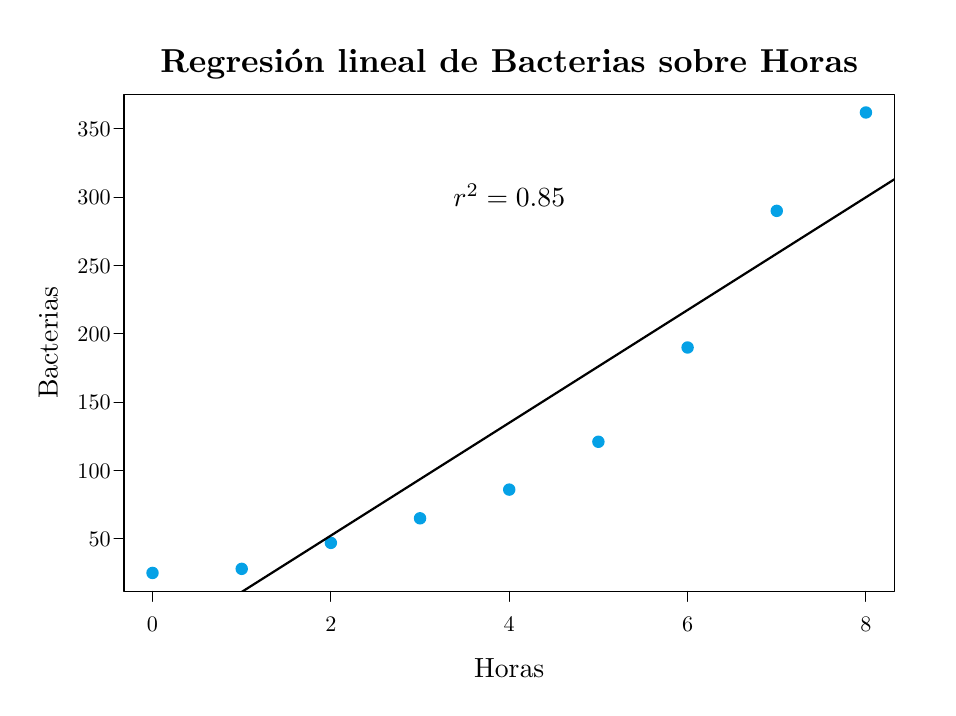
\begin{tikzpicture}[x=1pt,y=1pt]
\definecolor{fillColor}{RGB}{255,255,255}
\path[use as bounding box,fill=fillColor,fill opacity=0.00] (0,0) rectangle (325.21,238.49);
\begin{scope}
\path[clip] ( 34.80, 34.80) rectangle (313.21,214.49);
\definecolor{fillColor}{RGB}{5,161,230}

\path[fill=fillColor] ( 45.11, 41.46) circle (  2.25);

\path[fill=fillColor] ( 77.34, 42.94) circle (  2.25);

\path[fill=fillColor] (109.56, 52.32) circle (  2.25);

\path[fill=fillColor] (141.78, 61.20) circle (  2.25);

\path[fill=fillColor] (174.01, 71.57) circle (  2.25);

\path[fill=fillColor] (206.23, 88.85) circle (  2.25);

\path[fill=fillColor] (238.46,122.92) circle (  2.25);

\path[fill=fillColor] (270.68,172.29) circle (  2.25);

\path[fill=fillColor] (302.90,207.84) circle (  2.25);
\end{scope}
\begin{scope}
\path[clip] (  0.00,  0.00) rectangle (325.21,238.49);
\definecolor{drawColor}{RGB}{0,0,0}

\path[draw=drawColor,line width= 0.4pt,line join=round,line cap=round] ( 45.11, 34.80) -- (302.90, 34.80);

\path[draw=drawColor,line width= 0.4pt,line join=round,line cap=round] ( 45.11, 34.80) -- ( 45.11, 31.21);

\path[draw=drawColor,line width= 0.4pt,line join=round,line cap=round] (109.56, 34.80) -- (109.56, 31.21);

\path[draw=drawColor,line width= 0.4pt,line join=round,line cap=round] (174.01, 34.80) -- (174.01, 31.21);

\path[draw=drawColor,line width= 0.4pt,line join=round,line cap=round] (238.46, 34.80) -- (238.46, 31.21);

\path[draw=drawColor,line width= 0.4pt,line join=round,line cap=round] (302.90, 34.80) -- (302.90, 31.21);

\node[text=drawColor,anchor=base,inner sep=0pt, outer sep=0pt, scale=  0.80] at ( 45.11, 20.40) {0};

\node[text=drawColor,anchor=base,inner sep=0pt, outer sep=0pt, scale=  0.80] at (109.56, 20.40) {2};

\node[text=drawColor,anchor=base,inner sep=0pt, outer sep=0pt, scale=  0.80] at (174.01, 20.40) {4};

\node[text=drawColor,anchor=base,inner sep=0pt, outer sep=0pt, scale=  0.80] at (238.46, 20.40) {6};

\node[text=drawColor,anchor=base,inner sep=0pt, outer sep=0pt, scale=  0.80] at (302.90, 20.40) {8};

\path[draw=drawColor,line width= 0.4pt,line join=round,line cap=round] ( 34.80, 53.80) -- ( 34.80,201.91);

\path[draw=drawColor,line width= 0.4pt,line join=round,line cap=round] ( 34.80, 53.80) -- ( 31.21, 53.80);

\path[draw=drawColor,line width= 0.4pt,line join=round,line cap=round] ( 34.80, 78.48) -- ( 31.21, 78.48);

\path[draw=drawColor,line width= 0.4pt,line join=round,line cap=round] ( 34.80,103.17) -- ( 31.21,103.17);

\path[draw=drawColor,line width= 0.4pt,line join=round,line cap=round] ( 34.80,127.85) -- ( 31.21,127.85);

\path[draw=drawColor,line width= 0.4pt,line join=round,line cap=round] ( 34.80,152.54) -- ( 31.21,152.54);

\path[draw=drawColor,line width= 0.4pt,line join=round,line cap=round] ( 34.80,177.23) -- ( 31.21,177.23);

\path[draw=drawColor,line width= 0.4pt,line join=round,line cap=round] ( 34.80,201.91) -- ( 31.21,201.91);

\node[text=drawColor,anchor=base east,inner sep=0pt, outer sep=0pt, scale=  0.80] at ( 30.00, 51.04) {50};

\node[text=drawColor,anchor=base east,inner sep=0pt, outer sep=0pt, scale=  0.80] at ( 30.00, 75.73) {100};

\node[text=drawColor,anchor=base east,inner sep=0pt, outer sep=0pt, scale=  0.80] at ( 30.00,100.41) {150};

\node[text=drawColor,anchor=base east,inner sep=0pt, outer sep=0pt, scale=  0.80] at ( 30.00,125.10) {200};

\node[text=drawColor,anchor=base east,inner sep=0pt, outer sep=0pt, scale=  0.80] at ( 30.00,149.78) {250};

\node[text=drawColor,anchor=base east,inner sep=0pt, outer sep=0pt, scale=  0.80] at ( 30.00,174.47) {300};

\node[text=drawColor,anchor=base east,inner sep=0pt, outer sep=0pt, scale=  0.80] at ( 30.00,199.16) {350};

\path[draw=drawColor,line width= 0.4pt,line join=round,line cap=round] ( 34.80, 34.80) --
	(313.21, 34.80) --
	(313.21,214.49) --
	( 34.80,214.49) --
	( 34.80, 34.80);
\end{scope}
\begin{scope}
\path[clip] (  0.00,  0.00) rectangle (325.21,238.49);
\definecolor{drawColor}{RGB}{0,0,0}

\node[text=drawColor,anchor=base,inner sep=0pt, outer sep=0pt, scale=  1.20] at (174.01,222.30) {\bfseries Regresión lineal de Bacterias sobre Horas};

\node[text=drawColor,anchor=base,inner sep=0pt, outer sep=0pt, scale=  1.00] at (174.01,  3.60) {Horas};

\node[text=drawColor,rotate= 90.00,anchor=base,inner sep=0pt, outer sep=0pt, scale=  1.00] at ( 10.80,124.65) {Bacterias};
\end{scope}
\begin{scope}
\path[clip] ( 34.80, 34.80) rectangle (313.21,214.49);
\definecolor{drawColor}{RGB}{0,0,0}

\path[draw=drawColor,line width= 0.8pt,line join=round,line cap=round] ( 34.80,  7.69) -- (313.21,183.72);

\node[text=drawColor,anchor=base,inner sep=0pt, outer sep=0pt, scale=  1.00] at (174.01,173.76) {$r^2=0.85$};
\end{scope}
\end{tikzpicture}
}}
\mode<presentation>{\resizebox{0.9\textwidth}{!}{% Created by tikzDevice version 0.10.1 on 2016-02-27 13:16:26
% !TEX encoding = UTF-8 Unicode
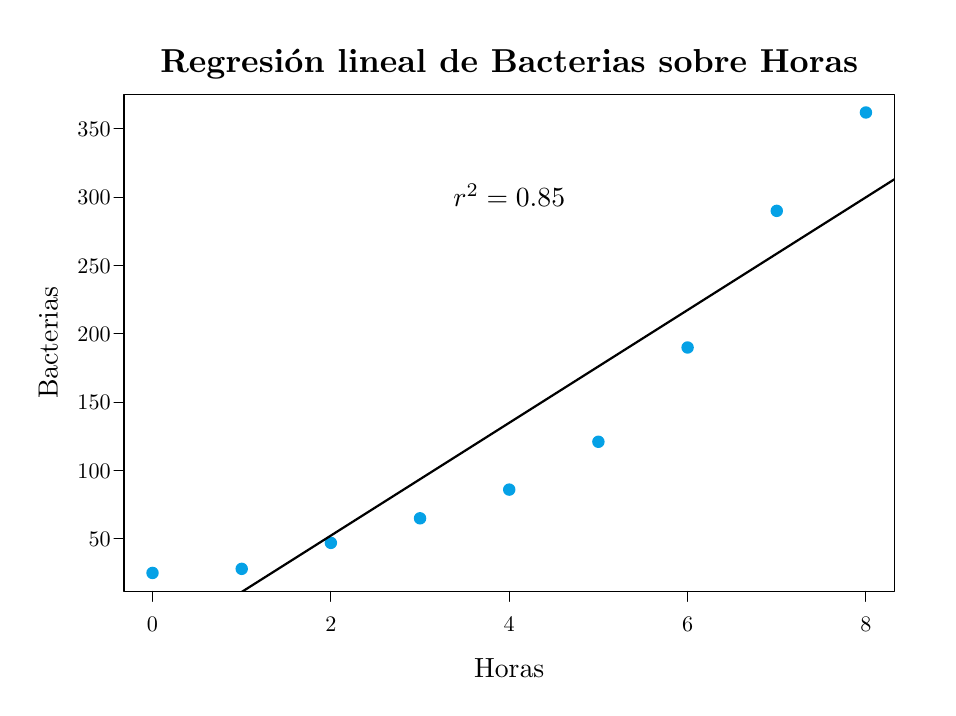
\begin{tikzpicture}[x=1pt,y=1pt]
\definecolor{fillColor}{RGB}{255,255,255}
\path[use as bounding box,fill=fillColor,fill opacity=0.00] (0,0) rectangle (325.21,238.49);
\begin{scope}
\path[clip] ( 34.80, 34.80) rectangle (313.21,214.49);
\definecolor{fillColor}{RGB}{5,161,230}

\path[fill=fillColor] ( 45.11, 41.46) circle (  2.25);

\path[fill=fillColor] ( 77.34, 42.94) circle (  2.25);

\path[fill=fillColor] (109.56, 52.32) circle (  2.25);

\path[fill=fillColor] (141.78, 61.20) circle (  2.25);

\path[fill=fillColor] (174.01, 71.57) circle (  2.25);

\path[fill=fillColor] (206.23, 88.85) circle (  2.25);

\path[fill=fillColor] (238.46,122.92) circle (  2.25);

\path[fill=fillColor] (270.68,172.29) circle (  2.25);

\path[fill=fillColor] (302.90,207.84) circle (  2.25);
\end{scope}
\begin{scope}
\path[clip] (  0.00,  0.00) rectangle (325.21,238.49);
\definecolor{drawColor}{RGB}{0,0,0}

\path[draw=drawColor,line width= 0.4pt,line join=round,line cap=round] ( 45.11, 34.80) -- (302.90, 34.80);

\path[draw=drawColor,line width= 0.4pt,line join=round,line cap=round] ( 45.11, 34.80) -- ( 45.11, 31.21);

\path[draw=drawColor,line width= 0.4pt,line join=round,line cap=round] (109.56, 34.80) -- (109.56, 31.21);

\path[draw=drawColor,line width= 0.4pt,line join=round,line cap=round] (174.01, 34.80) -- (174.01, 31.21);

\path[draw=drawColor,line width= 0.4pt,line join=round,line cap=round] (238.46, 34.80) -- (238.46, 31.21);

\path[draw=drawColor,line width= 0.4pt,line join=round,line cap=round] (302.90, 34.80) -- (302.90, 31.21);

\node[text=drawColor,anchor=base,inner sep=0pt, outer sep=0pt, scale=  0.80] at ( 45.11, 20.40) {0};

\node[text=drawColor,anchor=base,inner sep=0pt, outer sep=0pt, scale=  0.80] at (109.56, 20.40) {2};

\node[text=drawColor,anchor=base,inner sep=0pt, outer sep=0pt, scale=  0.80] at (174.01, 20.40) {4};

\node[text=drawColor,anchor=base,inner sep=0pt, outer sep=0pt, scale=  0.80] at (238.46, 20.40) {6};

\node[text=drawColor,anchor=base,inner sep=0pt, outer sep=0pt, scale=  0.80] at (302.90, 20.40) {8};

\path[draw=drawColor,line width= 0.4pt,line join=round,line cap=round] ( 34.80, 53.80) -- ( 34.80,201.91);

\path[draw=drawColor,line width= 0.4pt,line join=round,line cap=round] ( 34.80, 53.80) -- ( 31.21, 53.80);

\path[draw=drawColor,line width= 0.4pt,line join=round,line cap=round] ( 34.80, 78.48) -- ( 31.21, 78.48);

\path[draw=drawColor,line width= 0.4pt,line join=round,line cap=round] ( 34.80,103.17) -- ( 31.21,103.17);

\path[draw=drawColor,line width= 0.4pt,line join=round,line cap=round] ( 34.80,127.85) -- ( 31.21,127.85);

\path[draw=drawColor,line width= 0.4pt,line join=round,line cap=round] ( 34.80,152.54) -- ( 31.21,152.54);

\path[draw=drawColor,line width= 0.4pt,line join=round,line cap=round] ( 34.80,177.23) -- ( 31.21,177.23);

\path[draw=drawColor,line width= 0.4pt,line join=round,line cap=round] ( 34.80,201.91) -- ( 31.21,201.91);

\node[text=drawColor,anchor=base east,inner sep=0pt, outer sep=0pt, scale=  0.80] at ( 30.00, 51.04) {50};

\node[text=drawColor,anchor=base east,inner sep=0pt, outer sep=0pt, scale=  0.80] at ( 30.00, 75.73) {100};

\node[text=drawColor,anchor=base east,inner sep=0pt, outer sep=0pt, scale=  0.80] at ( 30.00,100.41) {150};

\node[text=drawColor,anchor=base east,inner sep=0pt, outer sep=0pt, scale=  0.80] at ( 30.00,125.10) {200};

\node[text=drawColor,anchor=base east,inner sep=0pt, outer sep=0pt, scale=  0.80] at ( 30.00,149.78) {250};

\node[text=drawColor,anchor=base east,inner sep=0pt, outer sep=0pt, scale=  0.80] at ( 30.00,174.47) {300};

\node[text=drawColor,anchor=base east,inner sep=0pt, outer sep=0pt, scale=  0.80] at ( 30.00,199.16) {350};

\path[draw=drawColor,line width= 0.4pt,line join=round,line cap=round] ( 34.80, 34.80) --
	(313.21, 34.80) --
	(313.21,214.49) --
	( 34.80,214.49) --
	( 34.80, 34.80);
\end{scope}
\begin{scope}
\path[clip] (  0.00,  0.00) rectangle (325.21,238.49);
\definecolor{drawColor}{RGB}{0,0,0}

\node[text=drawColor,anchor=base,inner sep=0pt, outer sep=0pt, scale=  1.20] at (174.01,222.30) {\bfseries Regresión lineal de Bacterias sobre Horas};

\node[text=drawColor,anchor=base,inner sep=0pt, outer sep=0pt, scale=  1.00] at (174.01,  3.60) {Horas};

\node[text=drawColor,rotate= 90.00,anchor=base,inner sep=0pt, outer sep=0pt, scale=  1.00] at ( 10.80,124.65) {Bacterias};
\end{scope}
\begin{scope}
\path[clip] ( 34.80, 34.80) rectangle (313.21,214.49);
\definecolor{drawColor}{RGB}{0,0,0}

\path[draw=drawColor,line width= 0.8pt,line join=round,line cap=round] ( 34.80,  7.69) -- (313.21,183.72);

\node[text=drawColor,anchor=base,inner sep=0pt, outer sep=0pt, scale=  1.00] at (174.01,173.76) {$r^2=0.85$};
\end{scope}
\end{tikzpicture}
}}
\end{center}
\end{column}
\end{columns}
\begin{center}
\emph{¿Es un buen modelo?}
\end{center}

\note{Si se calcula la recta de regresión del número de bacterias sobre las horas transcurridas, se observa que no es un mal modelo ya que
su coefiente de determinación lineal vale $0.85$. Ahora bien, que sea un buen modelo, no quiere decir que sea el mejor.
}
\end{frame}


%---------------------------------------------------------------------slide----
\begin{frame}
\frametitle{Ajuste de un modelo de regresión exponencial}
\framesubtitle{Evolución del número de bacterias de un cultivo}
Aunque el modelo lineal no es malo, de acuerdo al diagrama de dispersión es más lógico construir un modelo exponencial o cuadrático.

Para construir el modelo exponencial $y = ae^{bx}$ hay que realizar la transformación $z=\log y$, es decir, aplicar el logaritmo a la variable dependiente.

\begin{columns}
\begin{column}{0.45\textwidth}
\[
\begin{array}{c|c|c}
\mbox{Horas} & \mbox{Bacterias} & \mbox{Log Bacterias}\\
\hline
0 &  25 & 3.22\\
1 & 28 & 3.33\\
2 &  47 & 3.85\\
3 & 65  & 4.17\\
4 & 86 & 4.45\\
5 & 121 & 4.80\\
6 & 190 & 5.25\\
7 & 290 & 5.67\\
8 & 362 & 5.89
\end{array}
\]
\end{column}
\begin{column}{0.55\textwidth}
\begin{center}
\tikzsetnextfilename{regresion/evolucion_log_bacterias}
\mode<article>{\resizebox{0.7\textwidth}{!}{% Created by tikzDevice version 0.10.1 on 2016-02-27 13:16:44
% !TEX encoding = UTF-8 Unicode
\begin{tikzpicture}[x=1pt,y=1pt]
\definecolor{fillColor}{RGB}{255,255,255}
\path[use as bounding box,fill=fillColor,fill opacity=0.00] (0,0) rectangle (325.21,238.49);
\begin{scope}
\path[clip] ( 34.80, 34.80) rectangle (313.21,214.49);
\definecolor{fillColor}{RGB}{5,161,230}

\path[fill=fillColor] ( 45.11, 41.46) circle (  2.25);

\path[fill=fillColor] ( 77.34, 48.51) circle (  2.25);

\path[fill=fillColor] (109.56, 80.75) circle (  2.25);

\path[fill=fillColor] (141.78,100.94) circle (  2.25);

\path[fill=fillColor] (174.01,118.36) circle (  2.25);

\path[fill=fillColor] (206.23,139.62) circle (  2.25);

\path[fill=fillColor] (238.46,167.71) circle (  2.25);

\path[fill=fillColor] (270.68,194.03) circle (  2.25);

\path[fill=fillColor] (302.90,207.84) circle (  2.25);
\end{scope}
\begin{scope}
\path[clip] (  0.00,  0.00) rectangle (325.21,238.49);
\definecolor{drawColor}{RGB}{0,0,0}

\path[draw=drawColor,line width= 0.4pt,line join=round,line cap=round] ( 45.11, 34.80) -- (302.90, 34.80);

\path[draw=drawColor,line width= 0.4pt,line join=round,line cap=round] ( 45.11, 34.80) -- ( 45.11, 31.21);

\path[draw=drawColor,line width= 0.4pt,line join=round,line cap=round] (109.56, 34.80) -- (109.56, 31.21);

\path[draw=drawColor,line width= 0.4pt,line join=round,line cap=round] (174.01, 34.80) -- (174.01, 31.21);

\path[draw=drawColor,line width= 0.4pt,line join=round,line cap=round] (238.46, 34.80) -- (238.46, 31.21);

\path[draw=drawColor,line width= 0.4pt,line join=round,line cap=round] (302.90, 34.80) -- (302.90, 31.21);

\node[text=drawColor,anchor=base,inner sep=0pt, outer sep=0pt, scale=  0.80] at ( 45.11, 20.40) {0};

\node[text=drawColor,anchor=base,inner sep=0pt, outer sep=0pt, scale=  0.80] at (109.56, 20.40) {2};

\node[text=drawColor,anchor=base,inner sep=0pt, outer sep=0pt, scale=  0.80] at (174.01, 20.40) {4};

\node[text=drawColor,anchor=base,inner sep=0pt, outer sep=0pt, scale=  0.80] at (238.46, 20.40) {6};

\node[text=drawColor,anchor=base,inner sep=0pt, outer sep=0pt, scale=  0.80] at (302.90, 20.40) {8};

\path[draw=drawColor,line width= 0.4pt,line join=round,line cap=round] ( 34.80, 58.96) -- ( 34.80,183.46);

\path[draw=drawColor,line width= 0.4pt,line join=round,line cap=round] ( 34.80, 58.96) -- ( 31.21, 58.96);

\path[draw=drawColor,line width= 0.4pt,line join=round,line cap=round] ( 34.80, 90.08) -- ( 31.21, 90.08);

\path[draw=drawColor,line width= 0.4pt,line join=round,line cap=round] ( 34.80,121.21) -- ( 31.21,121.21);

\path[draw=drawColor,line width= 0.4pt,line join=round,line cap=round] ( 34.80,152.33) -- ( 31.21,152.33);

\path[draw=drawColor,line width= 0.4pt,line join=round,line cap=round] ( 34.80,183.46) -- ( 31.21,183.46);

\node[text=drawColor,anchor=base east,inner sep=0pt, outer sep=0pt, scale=  0.80] at ( 30.00, 56.20) {3.5};

\node[text=drawColor,anchor=base east,inner sep=0pt, outer sep=0pt, scale=  0.80] at ( 30.00, 87.32) {4.0};

\node[text=drawColor,anchor=base east,inner sep=0pt, outer sep=0pt, scale=  0.80] at ( 30.00,118.45) {4.5};

\node[text=drawColor,anchor=base east,inner sep=0pt, outer sep=0pt, scale=  0.80] at ( 30.00,149.58) {5.0};

\node[text=drawColor,anchor=base east,inner sep=0pt, outer sep=0pt, scale=  0.80] at ( 30.00,180.70) {5.5};

\path[draw=drawColor,line width= 0.4pt,line join=round,line cap=round] ( 34.80, 34.80) --
	(313.21, 34.80) --
	(313.21,214.49) --
	( 34.80,214.49) --
	( 34.80, 34.80);
\end{scope}
\begin{scope}
\path[clip] (  0.00,  0.00) rectangle (325.21,238.49);
\definecolor{drawColor}{RGB}{0,0,0}

\node[text=drawColor,anchor=base,inner sep=0pt, outer sep=0pt, scale=  1.20] at (174.01,222.30) {\bfseries Evolución de $\log$(Bacterias)};

\node[text=drawColor,anchor=base,inner sep=0pt, outer sep=0pt, scale=  1.00] at (174.01,  3.60) {Horas};

\node[text=drawColor,rotate= 90.00,anchor=base,inner sep=0pt, outer sep=0pt, scale=  1.00] at ( 10.80,124.65) {$\log$(Bacterias)};
\end{scope}
\end{tikzpicture}
}}
\mode<presentation>{\resizebox{0.9\textwidth}{!}{% Created by tikzDevice version 0.10.1 on 2016-02-27 13:16:44
% !TEX encoding = UTF-8 Unicode
\begin{tikzpicture}[x=1pt,y=1pt]
\definecolor{fillColor}{RGB}{255,255,255}
\path[use as bounding box,fill=fillColor,fill opacity=0.00] (0,0) rectangle (325.21,238.49);
\begin{scope}
\path[clip] ( 34.80, 34.80) rectangle (313.21,214.49);
\definecolor{fillColor}{RGB}{5,161,230}

\path[fill=fillColor] ( 45.11, 41.46) circle (  2.25);

\path[fill=fillColor] ( 77.34, 48.51) circle (  2.25);

\path[fill=fillColor] (109.56, 80.75) circle (  2.25);

\path[fill=fillColor] (141.78,100.94) circle (  2.25);

\path[fill=fillColor] (174.01,118.36) circle (  2.25);

\path[fill=fillColor] (206.23,139.62) circle (  2.25);

\path[fill=fillColor] (238.46,167.71) circle (  2.25);

\path[fill=fillColor] (270.68,194.03) circle (  2.25);

\path[fill=fillColor] (302.90,207.84) circle (  2.25);
\end{scope}
\begin{scope}
\path[clip] (  0.00,  0.00) rectangle (325.21,238.49);
\definecolor{drawColor}{RGB}{0,0,0}

\path[draw=drawColor,line width= 0.4pt,line join=round,line cap=round] ( 45.11, 34.80) -- (302.90, 34.80);

\path[draw=drawColor,line width= 0.4pt,line join=round,line cap=round] ( 45.11, 34.80) -- ( 45.11, 31.21);

\path[draw=drawColor,line width= 0.4pt,line join=round,line cap=round] (109.56, 34.80) -- (109.56, 31.21);

\path[draw=drawColor,line width= 0.4pt,line join=round,line cap=round] (174.01, 34.80) -- (174.01, 31.21);

\path[draw=drawColor,line width= 0.4pt,line join=round,line cap=round] (238.46, 34.80) -- (238.46, 31.21);

\path[draw=drawColor,line width= 0.4pt,line join=round,line cap=round] (302.90, 34.80) -- (302.90, 31.21);

\node[text=drawColor,anchor=base,inner sep=0pt, outer sep=0pt, scale=  0.80] at ( 45.11, 20.40) {0};

\node[text=drawColor,anchor=base,inner sep=0pt, outer sep=0pt, scale=  0.80] at (109.56, 20.40) {2};

\node[text=drawColor,anchor=base,inner sep=0pt, outer sep=0pt, scale=  0.80] at (174.01, 20.40) {4};

\node[text=drawColor,anchor=base,inner sep=0pt, outer sep=0pt, scale=  0.80] at (238.46, 20.40) {6};

\node[text=drawColor,anchor=base,inner sep=0pt, outer sep=0pt, scale=  0.80] at (302.90, 20.40) {8};

\path[draw=drawColor,line width= 0.4pt,line join=round,line cap=round] ( 34.80, 58.96) -- ( 34.80,183.46);

\path[draw=drawColor,line width= 0.4pt,line join=round,line cap=round] ( 34.80, 58.96) -- ( 31.21, 58.96);

\path[draw=drawColor,line width= 0.4pt,line join=round,line cap=round] ( 34.80, 90.08) -- ( 31.21, 90.08);

\path[draw=drawColor,line width= 0.4pt,line join=round,line cap=round] ( 34.80,121.21) -- ( 31.21,121.21);

\path[draw=drawColor,line width= 0.4pt,line join=round,line cap=round] ( 34.80,152.33) -- ( 31.21,152.33);

\path[draw=drawColor,line width= 0.4pt,line join=round,line cap=round] ( 34.80,183.46) -- ( 31.21,183.46);

\node[text=drawColor,anchor=base east,inner sep=0pt, outer sep=0pt, scale=  0.80] at ( 30.00, 56.20) {3.5};

\node[text=drawColor,anchor=base east,inner sep=0pt, outer sep=0pt, scale=  0.80] at ( 30.00, 87.32) {4.0};

\node[text=drawColor,anchor=base east,inner sep=0pt, outer sep=0pt, scale=  0.80] at ( 30.00,118.45) {4.5};

\node[text=drawColor,anchor=base east,inner sep=0pt, outer sep=0pt, scale=  0.80] at ( 30.00,149.58) {5.0};

\node[text=drawColor,anchor=base east,inner sep=0pt, outer sep=0pt, scale=  0.80] at ( 30.00,180.70) {5.5};

\path[draw=drawColor,line width= 0.4pt,line join=round,line cap=round] ( 34.80, 34.80) --
	(313.21, 34.80) --
	(313.21,214.49) --
	( 34.80,214.49) --
	( 34.80, 34.80);
\end{scope}
\begin{scope}
\path[clip] (  0.00,  0.00) rectangle (325.21,238.49);
\definecolor{drawColor}{RGB}{0,0,0}

\node[text=drawColor,anchor=base,inner sep=0pt, outer sep=0pt, scale=  1.20] at (174.01,222.30) {\bfseries Evolución de $\log$(Bacterias)};

\node[text=drawColor,anchor=base,inner sep=0pt, outer sep=0pt, scale=  1.00] at (174.01,  3.60) {Horas};

\node[text=drawColor,rotate= 90.00,anchor=base,inner sep=0pt, outer sep=0pt, scale=  1.00] at ( 10.80,124.65) {$\log$(Bacterias)};
\end{scope}
\end{tikzpicture}
}}
\end{center}
\end{column}
\end{columns}

\note{Para construir el modelo de regresión exponencial hay que aplicar el logaritmo neperiano a la variable dependiente, que en este caso
es el número de bacterias. El logaritmo neperiano de 25 nos da 3.22, el de 28 nos da 3.33 y así sucesivamente, de manera que obtenemos una
nueva variable que es el logarítmo de las bacterias. 

Si representamos el diagrama de dispersion del logaritmo de las bacterias y las horas transcurridas, podemos comprobar cómo ahora la nube de
puntos tiene forma lineal, es decir, mediante la transformación logarítmica de la variable dependiente hemos convertido una relación
exponencial en una relación lineal.
}
\end{frame}


%---------------------------------------------------------------------slide----
\begin{frame}
\frametitle{Ajuste de un modelo de regresión exponencial}
\framesubtitle{Evolución del número de bacterias de un cultivo}
Ahora sólo queda calcular la recta de regresión del logaritmo de Bacterias sobre Horas
\begin{columns}
\begin{column}{0.45\textwidth}
\[
\mbox{Log Bacterias} = 3.107 + 0.352\, \mbox{Horas}.
\]
Y deshaciendo el cambio de variable, se obtiene el modelo exponencial
\[
\mbox{Bacterias} = e^{3.107+0.352\,\textrm{Horas}}, \mbox{ con } r^2=0.99.
\]
Como se puede apreciar, el modelo exponencial se ajusta mucho mejor que el modelo lineal.
\end{column}
\begin{column}{0.55\textwidth}
\begin{center}
\tikzsetnextfilename{regresion/regresion_exponencial_bacterias}
\mode<article>{\resizebox{0.7\textwidth}{!}{% Created by tikzDevice version 0.10.1 on 2016-02-27 13:16:47
% !TEX encoding = UTF-8 Unicode
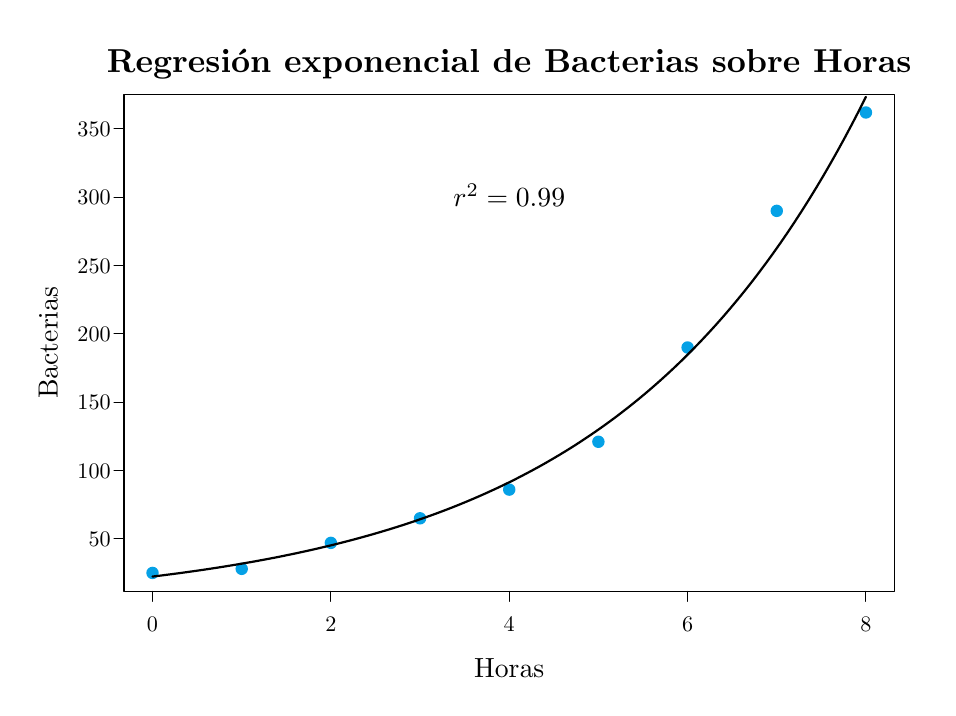
\begin{tikzpicture}[x=1pt,y=1pt]
\definecolor{fillColor}{RGB}{255,255,255}
\path[use as bounding box,fill=fillColor,fill opacity=0.00] (0,0) rectangle (325.21,238.49);
\begin{scope}
\path[clip] ( 34.80, 34.80) rectangle (313.21,214.49);
\definecolor{fillColor}{RGB}{5,161,230}

\path[fill=fillColor] ( 45.11, 41.46) circle (  2.25);

\path[fill=fillColor] ( 77.34, 42.94) circle (  2.25);

\path[fill=fillColor] (109.56, 52.32) circle (  2.25);

\path[fill=fillColor] (141.78, 61.20) circle (  2.25);

\path[fill=fillColor] (174.01, 71.57) circle (  2.25);

\path[fill=fillColor] (206.23, 88.85) circle (  2.25);

\path[fill=fillColor] (238.46,122.92) circle (  2.25);

\path[fill=fillColor] (270.68,172.29) circle (  2.25);

\path[fill=fillColor] (302.90,207.84) circle (  2.25);
\end{scope}
\begin{scope}
\path[clip] (  0.00,  0.00) rectangle (325.21,238.49);
\definecolor{drawColor}{RGB}{0,0,0}

\path[draw=drawColor,line width= 0.4pt,line join=round,line cap=round] ( 45.11, 34.80) -- (302.90, 34.80);

\path[draw=drawColor,line width= 0.4pt,line join=round,line cap=round] ( 45.11, 34.80) -- ( 45.11, 31.21);

\path[draw=drawColor,line width= 0.4pt,line join=round,line cap=round] (109.56, 34.80) -- (109.56, 31.21);

\path[draw=drawColor,line width= 0.4pt,line join=round,line cap=round] (174.01, 34.80) -- (174.01, 31.21);

\path[draw=drawColor,line width= 0.4pt,line join=round,line cap=round] (238.46, 34.80) -- (238.46, 31.21);

\path[draw=drawColor,line width= 0.4pt,line join=round,line cap=round] (302.90, 34.80) -- (302.90, 31.21);

\node[text=drawColor,anchor=base,inner sep=0pt, outer sep=0pt, scale=  0.80] at ( 45.11, 20.40) {0};

\node[text=drawColor,anchor=base,inner sep=0pt, outer sep=0pt, scale=  0.80] at (109.56, 20.40) {2};

\node[text=drawColor,anchor=base,inner sep=0pt, outer sep=0pt, scale=  0.80] at (174.01, 20.40) {4};

\node[text=drawColor,anchor=base,inner sep=0pt, outer sep=0pt, scale=  0.80] at (238.46, 20.40) {6};

\node[text=drawColor,anchor=base,inner sep=0pt, outer sep=0pt, scale=  0.80] at (302.90, 20.40) {8};

\path[draw=drawColor,line width= 0.4pt,line join=round,line cap=round] ( 34.80, 53.80) -- ( 34.80,201.91);

\path[draw=drawColor,line width= 0.4pt,line join=round,line cap=round] ( 34.80, 53.80) -- ( 31.21, 53.80);

\path[draw=drawColor,line width= 0.4pt,line join=round,line cap=round] ( 34.80, 78.48) -- ( 31.21, 78.48);

\path[draw=drawColor,line width= 0.4pt,line join=round,line cap=round] ( 34.80,103.17) -- ( 31.21,103.17);

\path[draw=drawColor,line width= 0.4pt,line join=round,line cap=round] ( 34.80,127.85) -- ( 31.21,127.85);

\path[draw=drawColor,line width= 0.4pt,line join=round,line cap=round] ( 34.80,152.54) -- ( 31.21,152.54);

\path[draw=drawColor,line width= 0.4pt,line join=round,line cap=round] ( 34.80,177.23) -- ( 31.21,177.23);

\path[draw=drawColor,line width= 0.4pt,line join=round,line cap=round] ( 34.80,201.91) -- ( 31.21,201.91);

\node[text=drawColor,anchor=base east,inner sep=0pt, outer sep=0pt, scale=  0.80] at ( 30.00, 51.04) {50};

\node[text=drawColor,anchor=base east,inner sep=0pt, outer sep=0pt, scale=  0.80] at ( 30.00, 75.73) {100};

\node[text=drawColor,anchor=base east,inner sep=0pt, outer sep=0pt, scale=  0.80] at ( 30.00,100.41) {150};

\node[text=drawColor,anchor=base east,inner sep=0pt, outer sep=0pt, scale=  0.80] at ( 30.00,125.10) {200};

\node[text=drawColor,anchor=base east,inner sep=0pt, outer sep=0pt, scale=  0.80] at ( 30.00,149.78) {250};

\node[text=drawColor,anchor=base east,inner sep=0pt, outer sep=0pt, scale=  0.80] at ( 30.00,174.47) {300};

\node[text=drawColor,anchor=base east,inner sep=0pt, outer sep=0pt, scale=  0.80] at ( 30.00,199.16) {350};

\path[draw=drawColor,line width= 0.4pt,line join=round,line cap=round] ( 34.80, 34.80) --
	(313.21, 34.80) --
	(313.21,214.49) --
	( 34.80,214.49) --
	( 34.80, 34.80);
\end{scope}
\begin{scope}
\path[clip] (  0.00,  0.00) rectangle (325.21,238.49);
\definecolor{drawColor}{RGB}{0,0,0}

\node[text=drawColor,anchor=base,inner sep=0pt, outer sep=0pt, scale=  1.20] at (174.01,222.30) {\bfseries Regresión exponencial de Bacterias sobre Horas};

\node[text=drawColor,anchor=base,inner sep=0pt, outer sep=0pt, scale=  1.00] at (174.01,  3.60) {Horas};

\node[text=drawColor,rotate= 90.00,anchor=base,inner sep=0pt, outer sep=0pt, scale=  1.00] at ( 10.80,124.65) {Bacterias};
\end{scope}
\begin{scope}
\path[clip] ( 34.80, 34.80) rectangle (313.21,214.49);
\definecolor{drawColor}{RGB}{0,0,0}

\path[draw=drawColor,line width= 0.8pt,line join=round,line cap=round] ( 45.11, 40.15) --
	( 47.69, 40.46) --
	( 50.27, 40.79) --
	( 52.85, 41.12) --
	( 55.42, 41.46) --
	( 58.00, 41.82) --
	( 60.58, 42.18) --
	( 63.16, 42.55) --
	( 65.73, 42.94) --
	( 68.31, 43.33) --
	( 70.89, 43.74) --
	( 73.47, 44.16) --
	( 76.05, 44.59) --
	( 78.62, 45.03) --
	( 81.20, 45.48) --
	( 83.78, 45.95) --
	( 86.36, 46.43) --
	( 88.94, 46.92) --
	( 91.51, 47.43) --
	( 94.09, 47.96) --
	( 96.67, 48.49) --
	( 99.25, 49.05) --
	(101.83, 49.62) --
	(104.40, 50.20) --
	(106.98, 50.81) --
	(109.56, 51.42) --
	(112.14, 52.06) --
	(114.72, 52.72) --
	(117.29, 53.39) --
	(119.87, 54.09) --
	(122.45, 54.80) --
	(125.03, 55.53) --
	(127.60, 56.29) --
	(130.18, 57.06) --
	(132.76, 57.86) --
	(135.34, 58.68) --
	(137.92, 59.53) --
	(140.49, 60.39) --
	(143.07, 61.29) --
	(145.65, 62.21) --
	(148.23, 63.15) --
	(150.81, 64.12) --
	(153.38, 65.12) --
	(155.96, 66.15) --
	(158.54, 67.21) --
	(161.12, 68.30) --
	(163.70, 69.42) --
	(166.27, 70.57) --
	(168.85, 71.75) --
	(171.43, 72.97) --
	(174.01, 74.22) --
	(176.59, 75.51) --
	(179.16, 76.84) --
	(181.74, 78.20) --
	(184.32, 79.60) --
	(186.90, 81.04) --
	(189.47, 82.53) --
	(192.05, 84.05) --
	(194.63, 85.62) --
	(197.21, 87.23) --
	(199.79, 88.89) --
	(202.36, 90.60) --
	(204.94, 92.36) --
	(207.52, 94.16) --
	(210.10, 96.02) --
	(212.68, 97.93) --
	(215.25, 99.90) --
	(217.83,101.92) --
	(220.41,104.00) --
	(222.99,106.14) --
	(225.57,108.34) --
	(228.14,110.60) --
	(230.72,112.93) --
	(233.30,115.32) --
	(235.88,117.78) --
	(238.46,120.32) --
	(241.03,122.92) --
	(243.61,125.60) --
	(246.19,128.36) --
	(248.77,131.19) --
	(251.34,134.10) --
	(253.92,137.10) --
	(256.50,140.19) --
	(259.08,143.36) --
	(261.66,146.62) --
	(264.23,149.98) --
	(266.81,153.43) --
	(269.39,156.98) --
	(271.97,160.63) --
	(274.55,164.39) --
	(277.12,168.25) --
	(279.70,172.23) --
	(282.28,176.31) --
	(284.86,180.52) --
	(287.44,184.84) --
	(290.01,189.29) --
	(292.59,193.86) --
	(295.17,198.57) --
	(297.75,203.41) --
	(300.33,208.39) --
	(302.90,213.51);

\node[text=drawColor,anchor=base,inner sep=0pt, outer sep=0pt, scale=  1.00] at (174.01,173.76) {$r^2=0.99$};
\end{scope}
\end{tikzpicture}
}}
\mode<presentation>{\resizebox{0.9\textwidth}{!}{% Created by tikzDevice version 0.10.1 on 2016-02-27 13:16:47
% !TEX encoding = UTF-8 Unicode
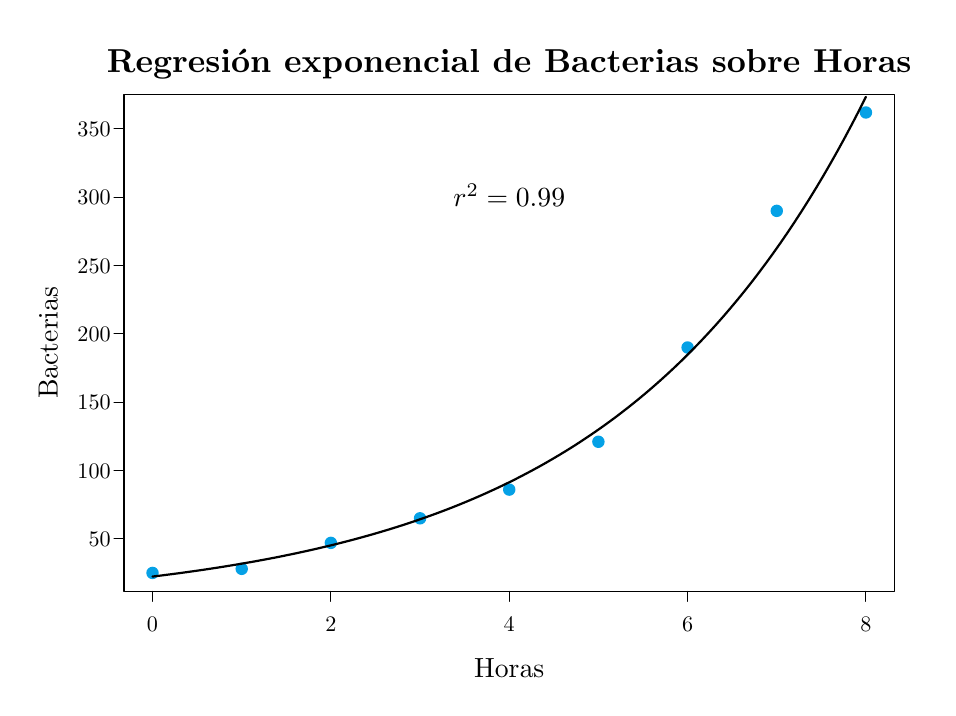
\begin{tikzpicture}[x=1pt,y=1pt]
\definecolor{fillColor}{RGB}{255,255,255}
\path[use as bounding box,fill=fillColor,fill opacity=0.00] (0,0) rectangle (325.21,238.49);
\begin{scope}
\path[clip] ( 34.80, 34.80) rectangle (313.21,214.49);
\definecolor{fillColor}{RGB}{5,161,230}

\path[fill=fillColor] ( 45.11, 41.46) circle (  2.25);

\path[fill=fillColor] ( 77.34, 42.94) circle (  2.25);

\path[fill=fillColor] (109.56, 52.32) circle (  2.25);

\path[fill=fillColor] (141.78, 61.20) circle (  2.25);

\path[fill=fillColor] (174.01, 71.57) circle (  2.25);

\path[fill=fillColor] (206.23, 88.85) circle (  2.25);

\path[fill=fillColor] (238.46,122.92) circle (  2.25);

\path[fill=fillColor] (270.68,172.29) circle (  2.25);

\path[fill=fillColor] (302.90,207.84) circle (  2.25);
\end{scope}
\begin{scope}
\path[clip] (  0.00,  0.00) rectangle (325.21,238.49);
\definecolor{drawColor}{RGB}{0,0,0}

\path[draw=drawColor,line width= 0.4pt,line join=round,line cap=round] ( 45.11, 34.80) -- (302.90, 34.80);

\path[draw=drawColor,line width= 0.4pt,line join=round,line cap=round] ( 45.11, 34.80) -- ( 45.11, 31.21);

\path[draw=drawColor,line width= 0.4pt,line join=round,line cap=round] (109.56, 34.80) -- (109.56, 31.21);

\path[draw=drawColor,line width= 0.4pt,line join=round,line cap=round] (174.01, 34.80) -- (174.01, 31.21);

\path[draw=drawColor,line width= 0.4pt,line join=round,line cap=round] (238.46, 34.80) -- (238.46, 31.21);

\path[draw=drawColor,line width= 0.4pt,line join=round,line cap=round] (302.90, 34.80) -- (302.90, 31.21);

\node[text=drawColor,anchor=base,inner sep=0pt, outer sep=0pt, scale=  0.80] at ( 45.11, 20.40) {0};

\node[text=drawColor,anchor=base,inner sep=0pt, outer sep=0pt, scale=  0.80] at (109.56, 20.40) {2};

\node[text=drawColor,anchor=base,inner sep=0pt, outer sep=0pt, scale=  0.80] at (174.01, 20.40) {4};

\node[text=drawColor,anchor=base,inner sep=0pt, outer sep=0pt, scale=  0.80] at (238.46, 20.40) {6};

\node[text=drawColor,anchor=base,inner sep=0pt, outer sep=0pt, scale=  0.80] at (302.90, 20.40) {8};

\path[draw=drawColor,line width= 0.4pt,line join=round,line cap=round] ( 34.80, 53.80) -- ( 34.80,201.91);

\path[draw=drawColor,line width= 0.4pt,line join=round,line cap=round] ( 34.80, 53.80) -- ( 31.21, 53.80);

\path[draw=drawColor,line width= 0.4pt,line join=round,line cap=round] ( 34.80, 78.48) -- ( 31.21, 78.48);

\path[draw=drawColor,line width= 0.4pt,line join=round,line cap=round] ( 34.80,103.17) -- ( 31.21,103.17);

\path[draw=drawColor,line width= 0.4pt,line join=round,line cap=round] ( 34.80,127.85) -- ( 31.21,127.85);

\path[draw=drawColor,line width= 0.4pt,line join=round,line cap=round] ( 34.80,152.54) -- ( 31.21,152.54);

\path[draw=drawColor,line width= 0.4pt,line join=round,line cap=round] ( 34.80,177.23) -- ( 31.21,177.23);

\path[draw=drawColor,line width= 0.4pt,line join=round,line cap=round] ( 34.80,201.91) -- ( 31.21,201.91);

\node[text=drawColor,anchor=base east,inner sep=0pt, outer sep=0pt, scale=  0.80] at ( 30.00, 51.04) {50};

\node[text=drawColor,anchor=base east,inner sep=0pt, outer sep=0pt, scale=  0.80] at ( 30.00, 75.73) {100};

\node[text=drawColor,anchor=base east,inner sep=0pt, outer sep=0pt, scale=  0.80] at ( 30.00,100.41) {150};

\node[text=drawColor,anchor=base east,inner sep=0pt, outer sep=0pt, scale=  0.80] at ( 30.00,125.10) {200};

\node[text=drawColor,anchor=base east,inner sep=0pt, outer sep=0pt, scale=  0.80] at ( 30.00,149.78) {250};

\node[text=drawColor,anchor=base east,inner sep=0pt, outer sep=0pt, scale=  0.80] at ( 30.00,174.47) {300};

\node[text=drawColor,anchor=base east,inner sep=0pt, outer sep=0pt, scale=  0.80] at ( 30.00,199.16) {350};

\path[draw=drawColor,line width= 0.4pt,line join=round,line cap=round] ( 34.80, 34.80) --
	(313.21, 34.80) --
	(313.21,214.49) --
	( 34.80,214.49) --
	( 34.80, 34.80);
\end{scope}
\begin{scope}
\path[clip] (  0.00,  0.00) rectangle (325.21,238.49);
\definecolor{drawColor}{RGB}{0,0,0}

\node[text=drawColor,anchor=base,inner sep=0pt, outer sep=0pt, scale=  1.20] at (174.01,222.30) {\bfseries Regresión exponencial de Bacterias sobre Horas};

\node[text=drawColor,anchor=base,inner sep=0pt, outer sep=0pt, scale=  1.00] at (174.01,  3.60) {Horas};

\node[text=drawColor,rotate= 90.00,anchor=base,inner sep=0pt, outer sep=0pt, scale=  1.00] at ( 10.80,124.65) {Bacterias};
\end{scope}
\begin{scope}
\path[clip] ( 34.80, 34.80) rectangle (313.21,214.49);
\definecolor{drawColor}{RGB}{0,0,0}

\path[draw=drawColor,line width= 0.8pt,line join=round,line cap=round] ( 45.11, 40.15) --
	( 47.69, 40.46) --
	( 50.27, 40.79) --
	( 52.85, 41.12) --
	( 55.42, 41.46) --
	( 58.00, 41.82) --
	( 60.58, 42.18) --
	( 63.16, 42.55) --
	( 65.73, 42.94) --
	( 68.31, 43.33) --
	( 70.89, 43.74) --
	( 73.47, 44.16) --
	( 76.05, 44.59) --
	( 78.62, 45.03) --
	( 81.20, 45.48) --
	( 83.78, 45.95) --
	( 86.36, 46.43) --
	( 88.94, 46.92) --
	( 91.51, 47.43) --
	( 94.09, 47.96) --
	( 96.67, 48.49) --
	( 99.25, 49.05) --
	(101.83, 49.62) --
	(104.40, 50.20) --
	(106.98, 50.81) --
	(109.56, 51.42) --
	(112.14, 52.06) --
	(114.72, 52.72) --
	(117.29, 53.39) --
	(119.87, 54.09) --
	(122.45, 54.80) --
	(125.03, 55.53) --
	(127.60, 56.29) --
	(130.18, 57.06) --
	(132.76, 57.86) --
	(135.34, 58.68) --
	(137.92, 59.53) --
	(140.49, 60.39) --
	(143.07, 61.29) --
	(145.65, 62.21) --
	(148.23, 63.15) --
	(150.81, 64.12) --
	(153.38, 65.12) --
	(155.96, 66.15) --
	(158.54, 67.21) --
	(161.12, 68.30) --
	(163.70, 69.42) --
	(166.27, 70.57) --
	(168.85, 71.75) --
	(171.43, 72.97) --
	(174.01, 74.22) --
	(176.59, 75.51) --
	(179.16, 76.84) --
	(181.74, 78.20) --
	(184.32, 79.60) --
	(186.90, 81.04) --
	(189.47, 82.53) --
	(192.05, 84.05) --
	(194.63, 85.62) --
	(197.21, 87.23) --
	(199.79, 88.89) --
	(202.36, 90.60) --
	(204.94, 92.36) --
	(207.52, 94.16) --
	(210.10, 96.02) --
	(212.68, 97.93) --
	(215.25, 99.90) --
	(217.83,101.92) --
	(220.41,104.00) --
	(222.99,106.14) --
	(225.57,108.34) --
	(228.14,110.60) --
	(230.72,112.93) --
	(233.30,115.32) --
	(235.88,117.78) --
	(238.46,120.32) --
	(241.03,122.92) --
	(243.61,125.60) --
	(246.19,128.36) --
	(248.77,131.19) --
	(251.34,134.10) --
	(253.92,137.10) --
	(256.50,140.19) --
	(259.08,143.36) --
	(261.66,146.62) --
	(264.23,149.98) --
	(266.81,153.43) --
	(269.39,156.98) --
	(271.97,160.63) --
	(274.55,164.39) --
	(277.12,168.25) --
	(279.70,172.23) --
	(282.28,176.31) --
	(284.86,180.52) --
	(287.44,184.84) --
	(290.01,189.29) --
	(292.59,193.86) --
	(295.17,198.57) --
	(297.75,203.41) --
	(300.33,208.39) --
	(302.90,213.51);

\node[text=drawColor,anchor=base,inner sep=0pt, outer sep=0pt, scale=  1.00] at (174.01,173.76) {$r^2=0.99$};
\end{scope}
\end{tikzpicture}
}}
\end{center}
\end{column}
\end{columns}

\note{Si ahora calculamos la recta de regresión del logaritmo de las bacterias sobre las horas, se tiene $\mbox{Log Bacterias} = 3.107 +
0.352\, \mbox{Horas}$, cuyo coeficiente de determinación lineal vale $0.99$, lo cual indica un ajuste casi perfecto de la recta. 

Finalmente, para obtener el modelo exponencial, basta con desacer la transformación logarítmica del número de bacterias, aplicando la
función exponencial, lo que nos da $\mbox{Bacterias} = e^{3.107+0.352\,\textrm{Horas}}$, y cuyo coeficiente de determinación exponencial
coincide con el de la recta anterior, de manera que se puede concluir que el modelo exponencial explica muyo mejor la relación entre el
número de bacterias y las horas que el modelo lineal. }
\end{frame}


%---------------------------------------------------------------------slide----
\begin{frame}
\frametitle{Interpretación de un coeficiente de determinación pequeño}
Es importante señalar que cada modelo de regresión tiene su propio coeficiente de determinación.
Así, un coeficiente de determinación cercano a cero significa que no existe relación entre las variables del tipo planteado por el modelo, pero \emph{eso no quiere decir que las variables sean
independientes}, ya que puede existir relación de otro tipo.
\begin{center}
\tikzsetnextfilename{regresion/regresion_lineal_relacion_cuadratica}
\resizebox{0.49\textwidth}{!}{% Created by tikzDevice version 0.10.1 on 2016-02-27 13:23:43
% !TEX encoding = UTF-8 Unicode
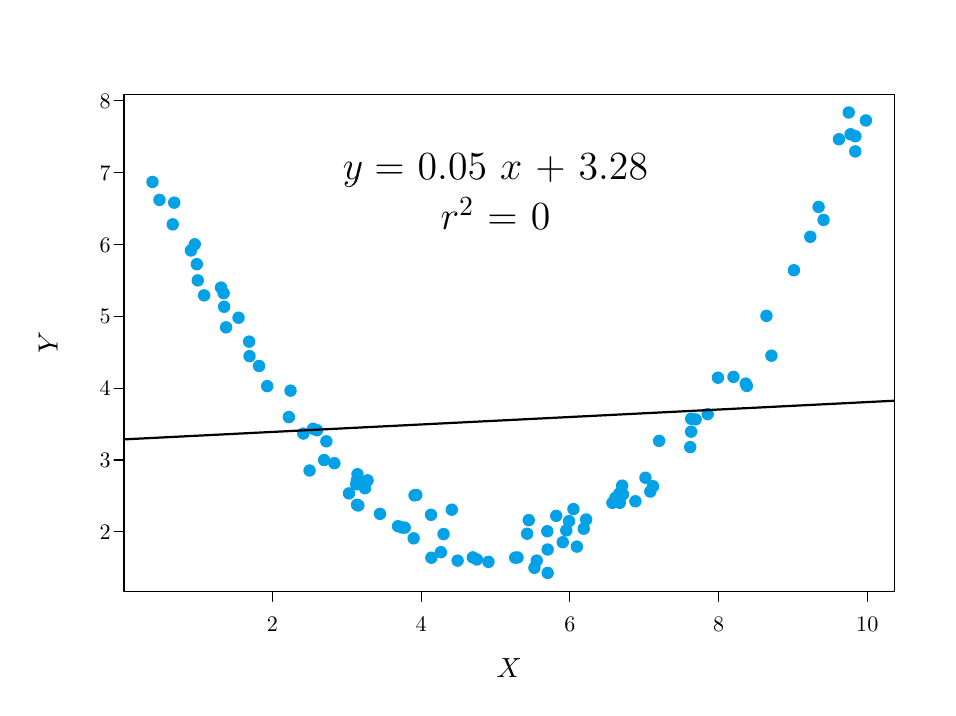
\begin{tikzpicture}[x=1pt,y=1pt]
\definecolor{fillColor}{RGB}{255,255,255}
\path[use as bounding box,fill=fillColor,fill opacity=0.00] (0,0) rectangle (325.21,238.49);
\begin{scope}
\path[clip] ( 34.80, 34.80) rectangle (313.21,214.49);
\definecolor{fillColor}{RGB}{5,161,230}

\path[fill=fillColor] ( 58.99,157.98) circle (  2.25);

\path[fill=fillColor] (139.47, 53.96) circle (  2.25);

\path[fill=fillColor] (297.34,199.97) circle (  2.25);

\path[fill=fillColor] (282.80,162.94) circle (  2.25);

\path[fill=fillColor] (119.48, 65.83) circle (  2.25);

\path[fill=fillColor] (287.59,169.01) circle (  2.25);

\path[fill=fillColor] (241.36, 96.94) circle (  2.25);

\path[fill=fillColor] (135.27, 57.88) circle (  2.25);

\path[fill=fillColor] (104.54, 93.04) circle (  2.25);

\path[fill=fillColor] (239.73, 92.50) circle (  2.25);

\path[fill=fillColor] (249.43,112.00) circle (  2.25);

\path[fill=fillColor] (195.62, 60.18) circle (  2.25);

\path[fill=fillColor] (119.18, 77.13) circle (  2.25);

\path[fill=fillColor] ( 83.60,116.24) circle (  2.25);

\path[fill=fillColor] (103.13, 93.56) circle (  2.25);

\path[fill=fillColor] (116.10, 70.20) circle (  2.25);

\path[fill=fillColor] (166.50, 45.46) circle (  2.25);

\path[fill=fillColor] (107.93, 89.02) circle (  2.25);

\path[fill=fillColor] (127.31, 62.80) circle (  2.25);

\path[fill=fillColor] (160.87, 47.09) circle (  2.25);

\path[fill=fillColor] ( 52.41,167.42) circle (  2.25);

\path[fill=fillColor] (201.81, 60.77) circle (  2.25);

\path[fill=fillColor] ( 61.13,153.03) circle (  2.25);

\path[fill=fillColor] (145.87, 46.96) circle (  2.25);

\path[fill=fillColor] (296.69,207.84) circle (  2.25);

\path[fill=fillColor] ( 52.95,175.26) circle (  2.25);

\path[fill=fillColor] (255.03,112.30) circle (  2.25);

\path[fill=fillColor] ( 69.87,144.57) circle (  2.25);

\path[fill=fillColor] ( 45.11,182.74) circle (  2.25);

\path[fill=fillColor] ( 70.81,142.54) circle (  2.25);

\path[fill=fillColor] (285.80,173.71) circle (  2.25);

\path[fill=fillColor] (239.41, 86.93) circle (  2.25);

\path[fill=fillColor] (213.96, 66.81) circle (  2.25);

\path[fill=fillColor] (122.82, 74.92) circle (  2.25);

\path[fill=fillColor] (187.90, 41.46) circle (  2.25);

\path[fill=fillColor] (118.71, 73.47) circle (  2.25);

\path[fill=fillColor] (183.95, 45.92) circle (  2.25);

\path[fill=fillColor] (194.62, 56.82) circle (  2.25);

\path[fill=fillColor] (153.26, 64.31) circle (  2.25);

\path[fill=fillColor] (119.02, 66.08) circle (  2.25);

\path[fill=fillColor] (145.74, 62.46) circle (  2.25);

\path[fill=fillColor] ( 70.98,137.64) circle (  2.25);

\path[fill=fillColor] (110.82, 81.11) circle (  2.25);

\path[fill=fillColor] (215.10, 69.84) circle (  2.25);

\path[fill=fillColor] (259.87,109.04) circle (  2.25);

\path[fill=fillColor] (191.00, 62.09) circle (  2.25);

\path[fill=fillColor] (155.36, 45.90) circle (  2.25);

\path[fill=fillColor] (214.81, 73.00) circle (  2.25);

\path[fill=fillColor] ( 63.75,141.76) circle (  2.25);

\path[fill=fillColor] (139.78, 69.49) circle (  2.25);

\path[fill=fillColor] (176.18, 46.98) circle (  2.25);

\path[fill=fillColor] (133.84, 58.33) circle (  2.25);

\path[fill=fillColor] (211.29, 66.80) circle (  2.25);

\path[fill=fillColor] (293.16,198.18) circle (  2.25);

\path[fill=fillColor] (177.01, 47.03) circle (  2.25);

\path[fill=fillColor] (181.05, 60.54) circle (  2.25);

\path[fill=fillColor] (150.28, 55.49) circle (  2.25);

\path[fill=fillColor] ( 61.47,147.17) circle (  2.25);

\path[fill=fillColor] (213.75, 70.13) circle (  2.25);

\path[fill=fillColor] ( 80.02,125.04) circle (  2.25);

\path[fill=fillColor] (193.35, 52.56) circle (  2.25);

\path[fill=fillColor] (187.90, 49.93) circle (  2.25);

\path[fill=fillColor] ( 71.69,130.20) circle (  2.25);

\path[fill=fillColor] (183.11, 43.32) circle (  2.25);

\path[fill=fillColor] ( 47.63,176.26) circle (  2.25);

\path[fill=fillColor] (200.93, 57.43) circle (  2.25);

\path[fill=fillColor] ( 94.98,107.32) circle (  2.25);

\path[fill=fillColor] (140.43, 69.62) circle (  2.25);

\path[fill=fillColor] (136.24, 57.82) circle (  2.25);

\path[fill=fillColor] ( 60.37,160.21) circle (  2.25);

\path[fill=fillColor] (225.96, 72.79) circle (  2.25);

\path[fill=fillColor] (266.95,134.35) circle (  2.25);

\path[fill=fillColor] ( 94.38, 97.78) circle (  2.25);

\path[fill=fillColor] ( 99.60, 91.82) circle (  2.25);

\path[fill=fillColor] (149.31, 48.94) circle (  2.25);

\path[fill=fillColor] ( 86.56,108.95) circle (  2.25);

\path[fill=fillColor] (107.10, 82.25) circle (  2.25);

\path[fill=fillColor] (101.86, 78.47) circle (  2.25);

\path[fill=fillColor] (224.98, 70.87) circle (  2.25);

\path[fill=fillColor] (121.91, 72.08) circle (  2.25);

\path[fill=fillColor] (212.38, 68.58) circle (  2.25);

\path[fill=fillColor] (239.75, 97.16) circle (  2.25);

\path[fill=fillColor] (228.18, 89.18) circle (  2.25);

\path[fill=fillColor] ( 80.17,119.79) circle (  2.25);

\path[fill=fillColor] (197.21, 64.53) circle (  2.25);

\path[fill=fillColor] (259.47,109.88) circle (  2.25);

\path[fill=fillColor] (245.71, 98.85) circle (  2.25);

\path[fill=fillColor] (162.32, 46.32) circle (  2.25);

\path[fill=fillColor] (302.90,204.96) circle (  2.25);

\path[fill=fillColor] (299.05,193.77) circle (  2.25);

\path[fill=fillColor] (276.89,150.83) circle (  2.25);

\path[fill=fillColor] (118.93, 74.87) circle (  2.25);

\path[fill=fillColor] (299.10,199.25) circle (  2.25);

\path[fill=fillColor] (198.46, 50.96) circle (  2.25);

\path[fill=fillColor] (180.48, 55.62) circle (  2.25);

\path[fill=fillColor] ( 76.20,133.68) circle (  2.25);

\path[fill=fillColor] (223.23, 75.85) circle (  2.25);

\path[fill=fillColor] (268.75,119.97) circle (  2.25);

\path[fill=fillColor] (219.60, 67.35) circle (  2.25);

\path[fill=fillColor] (187.77, 56.52) circle (  2.25);
\end{scope}
\begin{scope}
\path[clip] (  0.00,  0.00) rectangle (325.21,238.49);
\definecolor{drawColor}{RGB}{0,0,0}

\path[draw=drawColor,line width= 0.4pt,line join=round,line cap=round] ( 88.41, 34.80) -- (303.39, 34.80);

\path[draw=drawColor,line width= 0.4pt,line join=round,line cap=round] ( 88.41, 34.80) -- ( 88.41, 31.21);

\path[draw=drawColor,line width= 0.4pt,line join=round,line cap=round] (142.16, 34.80) -- (142.16, 31.21);

\path[draw=drawColor,line width= 0.4pt,line join=round,line cap=round] (195.90, 34.80) -- (195.90, 31.21);

\path[draw=drawColor,line width= 0.4pt,line join=round,line cap=round] (249.65, 34.80) -- (249.65, 31.21);

\path[draw=drawColor,line width= 0.4pt,line join=round,line cap=round] (303.39, 34.80) -- (303.39, 31.21);

\node[text=drawColor,anchor=base,inner sep=0pt, outer sep=0pt, scale=  0.80] at ( 88.41, 20.40) {2};

\node[text=drawColor,anchor=base,inner sep=0pt, outer sep=0pt, scale=  0.80] at (142.16, 20.40) {4};

\node[text=drawColor,anchor=base,inner sep=0pt, outer sep=0pt, scale=  0.80] at (195.90, 20.40) {6};

\node[text=drawColor,anchor=base,inner sep=0pt, outer sep=0pt, scale=  0.80] at (249.65, 20.40) {8};

\node[text=drawColor,anchor=base,inner sep=0pt, outer sep=0pt, scale=  0.80] at (303.39, 20.40) {10};

\path[draw=drawColor,line width= 0.4pt,line join=round,line cap=round] ( 34.80, 56.32) -- ( 34.80,212.09);

\path[draw=drawColor,line width= 0.4pt,line join=round,line cap=round] ( 34.80, 56.32) -- ( 31.21, 56.32);

\path[draw=drawColor,line width= 0.4pt,line join=round,line cap=round] ( 34.80, 82.28) -- ( 31.21, 82.28);

\path[draw=drawColor,line width= 0.4pt,line join=round,line cap=round] ( 34.80,108.25) -- ( 31.21,108.25);

\path[draw=drawColor,line width= 0.4pt,line join=round,line cap=round] ( 34.80,134.21) -- ( 31.21,134.21);

\path[draw=drawColor,line width= 0.4pt,line join=round,line cap=round] ( 34.80,160.17) -- ( 31.21,160.17);

\path[draw=drawColor,line width= 0.4pt,line join=round,line cap=round] ( 34.80,186.13) -- ( 31.21,186.13);

\path[draw=drawColor,line width= 0.4pt,line join=round,line cap=round] ( 34.80,212.09) -- ( 31.21,212.09);

\node[text=drawColor,anchor=base east,inner sep=0pt, outer sep=0pt, scale=  0.80] at ( 30.00, 53.57) {2};

\node[text=drawColor,anchor=base east,inner sep=0pt, outer sep=0pt, scale=  0.80] at ( 30.00, 79.53) {3};

\node[text=drawColor,anchor=base east,inner sep=0pt, outer sep=0pt, scale=  0.80] at ( 30.00,105.49) {4};

\node[text=drawColor,anchor=base east,inner sep=0pt, outer sep=0pt, scale=  0.80] at ( 30.00,131.45) {5};

\node[text=drawColor,anchor=base east,inner sep=0pt, outer sep=0pt, scale=  0.80] at ( 30.00,157.41) {6};

\node[text=drawColor,anchor=base east,inner sep=0pt, outer sep=0pt, scale=  0.80] at ( 30.00,183.37) {7};

\node[text=drawColor,anchor=base east,inner sep=0pt, outer sep=0pt, scale=  0.80] at ( 30.00,209.33) {8};

\path[draw=drawColor,line width= 0.4pt,line join=round,line cap=round] ( 34.80, 34.80) --
	(313.21, 34.80) --
	(313.21,214.49) --
	( 34.80,214.49) --
	( 34.80, 34.80);
\end{scope}
\begin{scope}
\path[clip] (  0.00,  0.00) rectangle (325.21,238.49);
\definecolor{drawColor}{RGB}{0,0,0}

\node[text=drawColor,anchor=base,inner sep=0pt, outer sep=0pt, scale=  1.00] at (174.01,  3.60) {$X$};

\node[text=drawColor,rotate= 90.00,anchor=base,inner sep=0pt, outer sep=0pt, scale=  1.00] at ( 10.80,124.65) {$Y$};
\end{scope}
\begin{scope}
\path[clip] ( 34.80, 34.80) rectangle (313.21,214.49);
\definecolor{drawColor}{RGB}{0,0,0}

\path[draw=drawColor,line width= 0.8pt,line join=round,line cap=round] ( 34.80, 89.72) -- (313.21,103.69);

\node[text=drawColor,anchor=base,inner sep=0pt, outer sep=0pt, scale=  1.00] at (169.03,183.63) {\Large $y=$ 0.05 $x$ + 3.28};

\node[text=drawColor,anchor=base,inner sep=0pt, outer sep=0pt, scale=  1.00] at (169.03,165.45) {\Large $r^2$ = 0};
\end{scope}
\end{tikzpicture}
}
\tikzsetnextfilename{regresion/regresion_cuadratica}
\resizebox{0.49\textwidth}{!}{% Created by tikzDevice version 0.10.1 on 2016-02-27 13:23:44
% !TEX encoding = UTF-8 Unicode
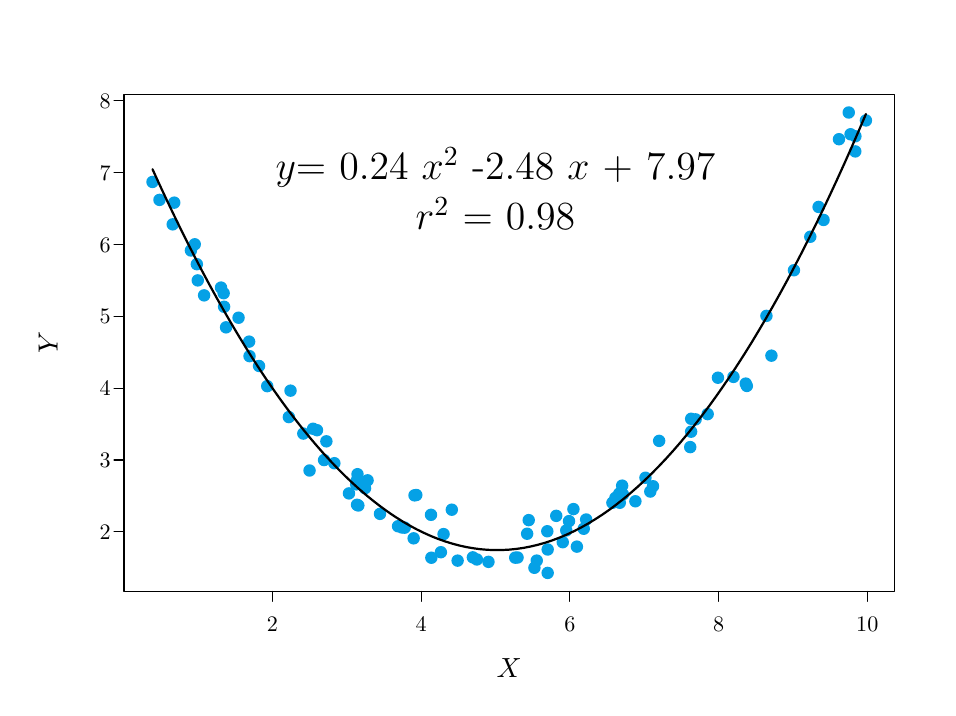
\begin{tikzpicture}[x=1pt,y=1pt]
\definecolor{fillColor}{RGB}{255,255,255}
\path[use as bounding box,fill=fillColor,fill opacity=0.00] (0,0) rectangle (325.21,238.49);
\begin{scope}
\path[clip] ( 34.80, 34.80) rectangle (313.21,214.49);
\definecolor{fillColor}{RGB}{5,161,230}

\path[fill=fillColor] ( 58.99,157.98) circle (  2.25);

\path[fill=fillColor] (139.47, 53.96) circle (  2.25);

\path[fill=fillColor] (297.34,199.97) circle (  2.25);

\path[fill=fillColor] (282.80,162.94) circle (  2.25);

\path[fill=fillColor] (119.48, 65.83) circle (  2.25);

\path[fill=fillColor] (287.59,169.01) circle (  2.25);

\path[fill=fillColor] (241.36, 96.94) circle (  2.25);

\path[fill=fillColor] (135.27, 57.88) circle (  2.25);

\path[fill=fillColor] (104.54, 93.04) circle (  2.25);

\path[fill=fillColor] (239.73, 92.50) circle (  2.25);

\path[fill=fillColor] (249.43,112.00) circle (  2.25);

\path[fill=fillColor] (195.62, 60.18) circle (  2.25);

\path[fill=fillColor] (119.18, 77.13) circle (  2.25);

\path[fill=fillColor] ( 83.60,116.24) circle (  2.25);

\path[fill=fillColor] (103.13, 93.56) circle (  2.25);

\path[fill=fillColor] (116.10, 70.20) circle (  2.25);

\path[fill=fillColor] (166.50, 45.46) circle (  2.25);

\path[fill=fillColor] (107.93, 89.02) circle (  2.25);

\path[fill=fillColor] (127.31, 62.80) circle (  2.25);

\path[fill=fillColor] (160.87, 47.09) circle (  2.25);

\path[fill=fillColor] ( 52.41,167.42) circle (  2.25);

\path[fill=fillColor] (201.81, 60.77) circle (  2.25);

\path[fill=fillColor] ( 61.13,153.03) circle (  2.25);

\path[fill=fillColor] (145.87, 46.96) circle (  2.25);

\path[fill=fillColor] (296.69,207.84) circle (  2.25);

\path[fill=fillColor] ( 52.95,175.26) circle (  2.25);

\path[fill=fillColor] (255.03,112.30) circle (  2.25);

\path[fill=fillColor] ( 69.87,144.57) circle (  2.25);

\path[fill=fillColor] ( 45.11,182.74) circle (  2.25);

\path[fill=fillColor] ( 70.81,142.54) circle (  2.25);

\path[fill=fillColor] (285.80,173.71) circle (  2.25);

\path[fill=fillColor] (239.41, 86.93) circle (  2.25);

\path[fill=fillColor] (213.96, 66.81) circle (  2.25);

\path[fill=fillColor] (122.82, 74.92) circle (  2.25);

\path[fill=fillColor] (187.90, 41.46) circle (  2.25);

\path[fill=fillColor] (118.71, 73.47) circle (  2.25);

\path[fill=fillColor] (183.95, 45.92) circle (  2.25);

\path[fill=fillColor] (194.62, 56.82) circle (  2.25);

\path[fill=fillColor] (153.26, 64.31) circle (  2.25);

\path[fill=fillColor] (119.02, 66.08) circle (  2.25);

\path[fill=fillColor] (145.74, 62.46) circle (  2.25);

\path[fill=fillColor] ( 70.98,137.64) circle (  2.25);

\path[fill=fillColor] (110.82, 81.11) circle (  2.25);

\path[fill=fillColor] (215.10, 69.84) circle (  2.25);

\path[fill=fillColor] (259.87,109.04) circle (  2.25);

\path[fill=fillColor] (191.00, 62.09) circle (  2.25);

\path[fill=fillColor] (155.36, 45.90) circle (  2.25);

\path[fill=fillColor] (214.81, 73.00) circle (  2.25);

\path[fill=fillColor] ( 63.75,141.76) circle (  2.25);

\path[fill=fillColor] (139.78, 69.49) circle (  2.25);

\path[fill=fillColor] (176.18, 46.98) circle (  2.25);

\path[fill=fillColor] (133.84, 58.33) circle (  2.25);

\path[fill=fillColor] (211.29, 66.80) circle (  2.25);

\path[fill=fillColor] (293.16,198.18) circle (  2.25);

\path[fill=fillColor] (177.01, 47.03) circle (  2.25);

\path[fill=fillColor] (181.05, 60.54) circle (  2.25);

\path[fill=fillColor] (150.28, 55.49) circle (  2.25);

\path[fill=fillColor] ( 61.47,147.17) circle (  2.25);

\path[fill=fillColor] (213.75, 70.13) circle (  2.25);

\path[fill=fillColor] ( 80.02,125.04) circle (  2.25);

\path[fill=fillColor] (193.35, 52.56) circle (  2.25);

\path[fill=fillColor] (187.90, 49.93) circle (  2.25);

\path[fill=fillColor] ( 71.69,130.20) circle (  2.25);

\path[fill=fillColor] (183.11, 43.32) circle (  2.25);

\path[fill=fillColor] ( 47.63,176.26) circle (  2.25);

\path[fill=fillColor] (200.93, 57.43) circle (  2.25);

\path[fill=fillColor] ( 94.98,107.32) circle (  2.25);

\path[fill=fillColor] (140.43, 69.62) circle (  2.25);

\path[fill=fillColor] (136.24, 57.82) circle (  2.25);

\path[fill=fillColor] ( 60.37,160.21) circle (  2.25);

\path[fill=fillColor] (225.96, 72.79) circle (  2.25);

\path[fill=fillColor] (266.95,134.35) circle (  2.25);

\path[fill=fillColor] ( 94.38, 97.78) circle (  2.25);

\path[fill=fillColor] ( 99.60, 91.82) circle (  2.25);

\path[fill=fillColor] (149.31, 48.94) circle (  2.25);

\path[fill=fillColor] ( 86.56,108.95) circle (  2.25);

\path[fill=fillColor] (107.10, 82.25) circle (  2.25);

\path[fill=fillColor] (101.86, 78.47) circle (  2.25);

\path[fill=fillColor] (224.98, 70.87) circle (  2.25);

\path[fill=fillColor] (121.91, 72.08) circle (  2.25);

\path[fill=fillColor] (212.38, 68.58) circle (  2.25);

\path[fill=fillColor] (239.75, 97.16) circle (  2.25);

\path[fill=fillColor] (228.18, 89.18) circle (  2.25);

\path[fill=fillColor] ( 80.17,119.79) circle (  2.25);

\path[fill=fillColor] (197.21, 64.53) circle (  2.25);

\path[fill=fillColor] (259.47,109.88) circle (  2.25);

\path[fill=fillColor] (245.71, 98.85) circle (  2.25);

\path[fill=fillColor] (162.32, 46.32) circle (  2.25);

\path[fill=fillColor] (302.90,204.96) circle (  2.25);

\path[fill=fillColor] (299.05,193.77) circle (  2.25);

\path[fill=fillColor] (276.89,150.83) circle (  2.25);

\path[fill=fillColor] (118.93, 74.87) circle (  2.25);

\path[fill=fillColor] (299.10,199.25) circle (  2.25);

\path[fill=fillColor] (198.46, 50.96) circle (  2.25);

\path[fill=fillColor] (180.48, 55.62) circle (  2.25);

\path[fill=fillColor] ( 76.20,133.68) circle (  2.25);

\path[fill=fillColor] (223.23, 75.85) circle (  2.25);

\path[fill=fillColor] (268.75,119.97) circle (  2.25);

\path[fill=fillColor] (219.60, 67.35) circle (  2.25);

\path[fill=fillColor] (187.77, 56.52) circle (  2.25);
\end{scope}
\begin{scope}
\path[clip] (  0.00,  0.00) rectangle (325.21,238.49);
\definecolor{drawColor}{RGB}{0,0,0}

\path[draw=drawColor,line width= 0.4pt,line join=round,line cap=round] ( 88.41, 34.80) -- (303.39, 34.80);

\path[draw=drawColor,line width= 0.4pt,line join=round,line cap=round] ( 88.41, 34.80) -- ( 88.41, 31.21);

\path[draw=drawColor,line width= 0.4pt,line join=round,line cap=round] (142.16, 34.80) -- (142.16, 31.21);

\path[draw=drawColor,line width= 0.4pt,line join=round,line cap=round] (195.90, 34.80) -- (195.90, 31.21);

\path[draw=drawColor,line width= 0.4pt,line join=round,line cap=round] (249.65, 34.80) -- (249.65, 31.21);

\path[draw=drawColor,line width= 0.4pt,line join=round,line cap=round] (303.39, 34.80) -- (303.39, 31.21);

\node[text=drawColor,anchor=base,inner sep=0pt, outer sep=0pt, scale=  0.80] at ( 88.41, 20.40) {2};

\node[text=drawColor,anchor=base,inner sep=0pt, outer sep=0pt, scale=  0.80] at (142.16, 20.40) {4};

\node[text=drawColor,anchor=base,inner sep=0pt, outer sep=0pt, scale=  0.80] at (195.90, 20.40) {6};

\node[text=drawColor,anchor=base,inner sep=0pt, outer sep=0pt, scale=  0.80] at (249.65, 20.40) {8};

\node[text=drawColor,anchor=base,inner sep=0pt, outer sep=0pt, scale=  0.80] at (303.39, 20.40) {10};

\path[draw=drawColor,line width= 0.4pt,line join=round,line cap=round] ( 34.80, 56.32) -- ( 34.80,212.09);

\path[draw=drawColor,line width= 0.4pt,line join=round,line cap=round] ( 34.80, 56.32) -- ( 31.21, 56.32);

\path[draw=drawColor,line width= 0.4pt,line join=round,line cap=round] ( 34.80, 82.28) -- ( 31.21, 82.28);

\path[draw=drawColor,line width= 0.4pt,line join=round,line cap=round] ( 34.80,108.25) -- ( 31.21,108.25);

\path[draw=drawColor,line width= 0.4pt,line join=round,line cap=round] ( 34.80,134.21) -- ( 31.21,134.21);

\path[draw=drawColor,line width= 0.4pt,line join=round,line cap=round] ( 34.80,160.17) -- ( 31.21,160.17);

\path[draw=drawColor,line width= 0.4pt,line join=round,line cap=round] ( 34.80,186.13) -- ( 31.21,186.13);

\path[draw=drawColor,line width= 0.4pt,line join=round,line cap=round] ( 34.80,212.09) -- ( 31.21,212.09);

\node[text=drawColor,anchor=base east,inner sep=0pt, outer sep=0pt, scale=  0.80] at ( 30.00, 53.57) {2};

\node[text=drawColor,anchor=base east,inner sep=0pt, outer sep=0pt, scale=  0.80] at ( 30.00, 79.53) {3};

\node[text=drawColor,anchor=base east,inner sep=0pt, outer sep=0pt, scale=  0.80] at ( 30.00,105.49) {4};

\node[text=drawColor,anchor=base east,inner sep=0pt, outer sep=0pt, scale=  0.80] at ( 30.00,131.45) {5};

\node[text=drawColor,anchor=base east,inner sep=0pt, outer sep=0pt, scale=  0.80] at ( 30.00,157.41) {6};

\node[text=drawColor,anchor=base east,inner sep=0pt, outer sep=0pt, scale=  0.80] at ( 30.00,183.37) {7};

\node[text=drawColor,anchor=base east,inner sep=0pt, outer sep=0pt, scale=  0.80] at ( 30.00,209.33) {8};

\path[draw=drawColor,line width= 0.4pt,line join=round,line cap=round] ( 34.80, 34.80) --
	(313.21, 34.80) --
	(313.21,214.49) --
	( 34.80,214.49) --
	( 34.80, 34.80);
\end{scope}
\begin{scope}
\path[clip] (  0.00,  0.00) rectangle (325.21,238.49);
\definecolor{drawColor}{RGB}{0,0,0}

\node[text=drawColor,anchor=base,inner sep=0pt, outer sep=0pt, scale=  1.00] at (174.01,  3.60) {$X$};

\node[text=drawColor,rotate= 90.00,anchor=base,inner sep=0pt, outer sep=0pt, scale=  1.00] at ( 10.80,124.65) {$Y$};
\end{scope}
\begin{scope}
\path[clip] ( 34.80, 34.80) rectangle (313.21,214.49);
\definecolor{drawColor}{RGB}{0,0,0}

\path[draw=drawColor,line width= 0.8pt,line join=round,line cap=round] ( 45.11,187.33) --
	( 47.69,181.69) --
	( 50.27,176.17) --
	( 52.85,170.77) --
	( 55.42,165.48) --
	( 58.00,160.31) --
	( 60.58,155.27) --
	( 63.16,150.33) --
	( 65.73,145.52) --
	( 68.31,140.83) --
	( 70.89,136.25) --
	( 73.47,131.79) --
	( 76.05,127.45) --
	( 78.62,123.23) --
	( 81.20,119.12) --
	( 83.78,115.13) --
	( 86.36,111.26) --
	( 88.94,107.51) --
	( 91.51,103.88) --
	( 94.09,100.36) --
	( 96.67, 96.97) --
	( 99.25, 93.69) --
	(101.83, 90.52) --
	(104.40, 87.48) --
	(106.98, 84.55) --
	(109.56, 81.75) --
	(112.14, 79.06) --
	(114.72, 76.48) --
	(117.29, 74.03) --
	(119.87, 71.69) --
	(122.45, 69.48) --
	(125.03, 67.38) --
	(127.61, 65.39) --
	(130.18, 63.53) --
	(132.76, 61.78) --
	(135.34, 60.15) --
	(137.92, 58.64) --
	(140.49, 57.25) --
	(143.07, 55.98) --
	(145.65, 54.82) --
	(148.23, 53.78) --
	(150.81, 52.86) --
	(153.38, 52.06) --
	(155.96, 51.37) --
	(158.54, 50.80) --
	(161.12, 50.36) --
	(163.70, 50.02) --
	(166.27, 49.81) --
	(168.85, 49.72) --
	(171.43, 49.74) --
	(174.01, 49.88) --
	(176.59, 50.14) --
	(179.16, 50.51) --
	(181.74, 51.01) --
	(184.32, 51.62) --
	(186.90, 52.35) --
	(189.47, 53.20) --
	(192.05, 54.17) --
	(194.63, 55.25) --
	(197.21, 56.45) --
	(199.79, 57.77) --
	(202.36, 59.21) --
	(204.94, 60.77) --
	(207.52, 62.44) --
	(210.10, 64.23) --
	(212.68, 66.14) --
	(215.25, 68.17) --
	(217.83, 70.32) --
	(220.41, 72.58) --
	(222.99, 74.96) --
	(225.57, 77.46) --
	(228.14, 80.08) --
	(230.72, 82.81) --
	(233.30, 85.67) --
	(235.88, 88.64) --
	(238.46, 91.73) --
	(241.03, 94.94) --
	(243.61, 98.26) --
	(246.19,101.70) --
	(248.77,105.27) --
	(251.34,108.94) --
	(253.92,112.74) --
	(256.50,116.66) --
	(259.08,120.69) --
	(261.66,124.84) --
	(264.23,129.11) --
	(266.81,133.50) --
	(269.39,138.00) --
	(271.97,142.62) --
	(274.55,147.36) --
	(277.12,152.22) --
	(279.70,157.20) --
	(282.28,162.29) --
	(284.86,167.51) --
	(287.44,172.84) --
	(290.01,178.28) --
	(292.59,183.85) --
	(295.17,189.53) --
	(297.75,195.34) --
	(300.33,201.26) --
	(302.90,207.29);

\node[text=drawColor,anchor=base,inner sep=0pt, outer sep=0pt, scale=  1.00] at (169.03,183.63) {\Large $y$= 0.24 $x^2$ -2.48 $x$ + 7.97};

\node[text=drawColor,anchor=base,inner sep=0pt, outer sep=0pt, scale=  1.00] at (169.03,165.45) {\Large $r^2$ = 0.98};
\end{scope}
\end{tikzpicture}
}
\end{center}

\note{Hay que recordar que tanto el coeficiente de determinación hace referencia a un modelo concreto, de manera que
un coeficiente $r^2=0$ significa que no existe relación entre las variables del tipo planteado por el modelo, pero \emph{eso no quiere decir
que las variables sean independientes}, ya que puede existir relación de otro tipo.

En las gráficas puede apreciarse cómo al ajustar una recta sobre esta nube de puntos se obtiene un coeficiente de determinación
prácticamente nulo pero sin embargo hay una clara relación parabólica entre las variables, por lo que no podemos decir que las variables
son independientes, tan sólo que no tienen relación lineal.}
\end{frame}


%---------------------------------------------------------------------slide----
\begin{frame}
\frametitle{Datos atípicos en regresión}
Los \emph{datos atípicos} en un estudio de regresión son los puntos que claramente no siguen la tendencia del resto de los puntos en el diagrama de dispersión, incluso si los valores del par no se pueden considerar atípicos para cada variable por separado.

\begin{center}
\tikzsetnextfilename{regresion/diagrama_dispersion_con_datos_atipicos}
\resizebox{0.7\textwidth}{!}{% Created by tikzDevice version 0.10.1 on 2016-02-27 13:47:46
% !TEX encoding = UTF-8 Unicode
\begin{tikzpicture}[x=1pt,y=1pt]
\definecolor{fillColor}{RGB}{255,255,255}
\path[use as bounding box,fill=fillColor,fill opacity=0.00] (0,0) rectangle (325.21,238.49);
\begin{scope}
\path[clip] ( 34.80, 34.80) rectangle (313.21,214.49);
\definecolor{fillColor}{RGB}{5,161,230}

\path[fill=fillColor] ( 72.15,118.24) circle (  2.25);

\path[fill=fillColor] (270.97, 51.29) circle (  2.25);

\path[fill=fillColor] ( 93.12,103.19) circle (  2.25);

\path[fill=fillColor] (146.01, 92.94) circle (  2.25);

\path[fill=fillColor] (211.70, 67.10) circle (  2.25);

\path[fill=fillColor] (149.78, 92.94) circle (  2.25);

\path[fill=fillColor] (289.83, 43.74) circle (  2.25);

\path[fill=fillColor] (300.55, 44.55) circle (  2.25);

\path[fill=fillColor] (121.56, 97.84) circle (  2.25);

\path[fill=fillColor] (251.34,174.56) circle (  2.25);
\end{scope}
\begin{scope}
\path[clip] (  0.00,  0.00) rectangle (325.21,238.49);
\definecolor{drawColor}{RGB}{0,0,0}

\path[draw=drawColor,line width= 0.4pt,line join=round,line cap=round] ( 45.11, 34.80) -- (302.90, 34.80);

\path[draw=drawColor,line width= 0.4pt,line join=round,line cap=round] ( 45.11, 34.80) -- ( 45.11, 31.21);

\path[draw=drawColor,line width= 0.4pt,line join=round,line cap=round] ( 96.67, 34.80) -- ( 96.67, 31.21);

\path[draw=drawColor,line width= 0.4pt,line join=round,line cap=round] (148.23, 34.80) -- (148.23, 31.21);

\path[draw=drawColor,line width= 0.4pt,line join=round,line cap=round] (199.79, 34.80) -- (199.79, 31.21);

\path[draw=drawColor,line width= 0.4pt,line join=round,line cap=round] (251.34, 34.80) -- (251.34, 31.21);

\path[draw=drawColor,line width= 0.4pt,line join=round,line cap=round] (302.90, 34.80) -- (302.90, 31.21);

\node[text=drawColor,anchor=base,inner sep=0pt, outer sep=0pt, scale=  0.80] at ( 45.11, 20.40) {0};

\node[text=drawColor,anchor=base,inner sep=0pt, outer sep=0pt, scale=  0.80] at ( 96.67, 20.40) {2};

\node[text=drawColor,anchor=base,inner sep=0pt, outer sep=0pt, scale=  0.80] at (148.23, 20.40) {4};

\node[text=drawColor,anchor=base,inner sep=0pt, outer sep=0pt, scale=  0.80] at (199.79, 20.40) {6};

\node[text=drawColor,anchor=base,inner sep=0pt, outer sep=0pt, scale=  0.80] at (251.34, 20.40) {8};

\node[text=drawColor,anchor=base,inner sep=0pt, outer sep=0pt, scale=  0.80] at (302.90, 20.40) {10};

\path[draw=drawColor,line width= 0.4pt,line join=round,line cap=round] ( 34.80, 41.46) -- ( 34.80,207.84);

\path[draw=drawColor,line width= 0.4pt,line join=round,line cap=round] ( 34.80, 41.46) -- ( 31.21, 41.46);

\path[draw=drawColor,line width= 0.4pt,line join=round,line cap=round] ( 34.80, 74.73) -- ( 31.21, 74.73);

\path[draw=drawColor,line width= 0.4pt,line join=round,line cap=round] ( 34.80,108.01) -- ( 31.21,108.01);

\path[draw=drawColor,line width= 0.4pt,line join=round,line cap=round] ( 34.80,141.28) -- ( 31.21,141.28);

\path[draw=drawColor,line width= 0.4pt,line join=round,line cap=round] ( 34.80,174.56) -- ( 31.21,174.56);

\path[draw=drawColor,line width= 0.4pt,line join=round,line cap=round] ( 34.80,207.84) -- ( 31.21,207.84);

\node[text=drawColor,anchor=base east,inner sep=0pt, outer sep=0pt, scale=  0.80] at ( 30.00, 38.70) {0};

\node[text=drawColor,anchor=base east,inner sep=0pt, outer sep=0pt, scale=  0.80] at ( 30.00, 71.98) {2};

\node[text=drawColor,anchor=base east,inner sep=0pt, outer sep=0pt, scale=  0.80] at ( 30.00,105.25) {4};

\node[text=drawColor,anchor=base east,inner sep=0pt, outer sep=0pt, scale=  0.80] at ( 30.00,138.53) {6};

\node[text=drawColor,anchor=base east,inner sep=0pt, outer sep=0pt, scale=  0.80] at ( 30.00,171.80) {8};

\node[text=drawColor,anchor=base east,inner sep=0pt, outer sep=0pt, scale=  0.80] at ( 30.00,205.08) {10};

\path[draw=drawColor,line width= 0.4pt,line join=round,line cap=round] ( 34.80, 34.80) --
	(313.21, 34.80) --
	(313.21,214.49) --
	( 34.80,214.49) --
	( 34.80, 34.80);
\end{scope}
\begin{scope}
\path[clip] (  0.00,  0.00) rectangle (325.21,238.49);
\definecolor{drawColor}{RGB}{0,0,0}

\node[text=drawColor,anchor=base,inner sep=0pt, outer sep=0pt, scale=  1.20] at (174.01,222.30) {\bfseries Diagrama de dispersión con datos atípicos};

\node[text=drawColor,anchor=base,inner sep=0pt, outer sep=0pt, scale=  1.00] at (174.01,  3.60) {$X$};

\node[text=drawColor,rotate= 90.00,anchor=base,inner sep=0pt, outer sep=0pt, scale=  1.00] at ( 10.80,124.65) {$Y$};
\end{scope}
\begin{scope}
\path[clip] ( 34.80, 34.80) rectangle (313.21,214.49);
\definecolor{fillColor}{RGB}{238,50,36}

\path[fill=fillColor] (251.34,174.56) circle (  2.25);
\definecolor{drawColor}{RGB}{0,0,0}

\node[text=drawColor,anchor=base,inner sep=0pt, outer sep=0pt, scale=  1.00] at (215.57,171.12) {Dato atípico};
\end{scope}
\end{tikzpicture}
}
\end{center}

\note{Otro de los problemas que pueden plantearse en la construcción de un modelo de regresión es la presencia de datos atípicos. En un
estudio de regresión, los datos atípicos, a diferencia de lo que vimos en el tema anterior no son individuos que presentan un valor en
alguna de las variables muy distinto del resto, sino que son puntos que se alejan notablemente de la tendencia de la nube de puntos.

Como se aprecia en el gráfico, aunque un individuo podría no ser un \emph{dato atípico} al considerar las variables de manera separada, sí
lo sería al considerarlas de manera conjunta.}
\end{frame}


%---------------------------------------------------------------------slide----
\begin{frame}
\frametitle{Influencia de los datos atípicos en los modelos de regresión}
Los datos atípicos en regresión suelen provocar cambios drásticos en el ajuste de los modelos de regresión, y por tanto, habrá que tener mucho cuidado con ellos.

\begin{center}
\tikzsetnextfilename{regresion/regresion_lineal_con_datos_atipicos}
\resizebox{0.49\textwidth}{!}{% Created by tikzDevice version 0.10.1 on 2016-02-27 13:34:00
% !TEX encoding = UTF-8 Unicode
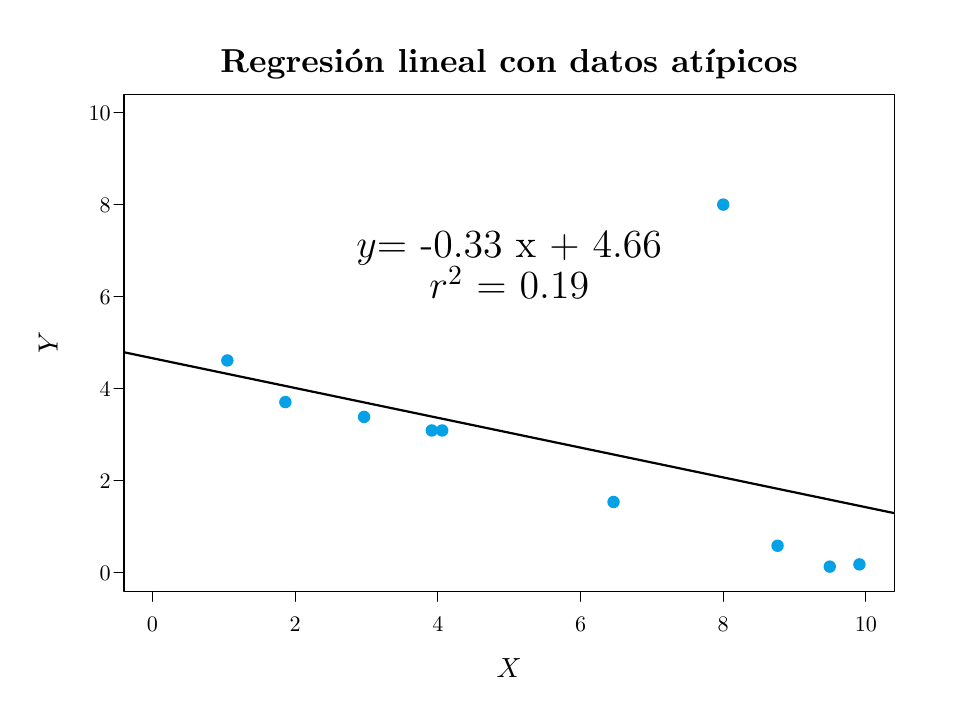
\begin{tikzpicture}[x=1pt,y=1pt]
\definecolor{fillColor}{RGB}{255,255,255}
\path[use as bounding box,fill=fillColor,fill opacity=0.00] (0,0) rectangle (325.21,238.49);
\begin{scope}
\path[clip] ( 34.80, 34.80) rectangle (313.21,214.49);
\definecolor{fillColor}{RGB}{5,161,230}

\path[fill=fillColor] ( 72.15,118.24) circle (  2.25);

\path[fill=fillColor] (270.97, 51.29) circle (  2.25);

\path[fill=fillColor] ( 93.12,103.19) circle (  2.25);

\path[fill=fillColor] (146.01, 92.94) circle (  2.25);

\path[fill=fillColor] (211.70, 67.10) circle (  2.25);

\path[fill=fillColor] (149.78, 92.94) circle (  2.25);

\path[fill=fillColor] (289.83, 43.74) circle (  2.25);

\path[fill=fillColor] (300.55, 44.55) circle (  2.25);

\path[fill=fillColor] (121.56, 97.84) circle (  2.25);

\path[fill=fillColor] (251.34,174.56) circle (  2.25);
\end{scope}
\begin{scope}
\path[clip] (  0.00,  0.00) rectangle (325.21,238.49);
\definecolor{drawColor}{RGB}{0,0,0}

\path[draw=drawColor,line width= 0.4pt,line join=round,line cap=round] ( 45.11, 34.80) -- (302.90, 34.80);

\path[draw=drawColor,line width= 0.4pt,line join=round,line cap=round] ( 45.11, 34.80) -- ( 45.11, 31.21);

\path[draw=drawColor,line width= 0.4pt,line join=round,line cap=round] ( 96.67, 34.80) -- ( 96.67, 31.21);

\path[draw=drawColor,line width= 0.4pt,line join=round,line cap=round] (148.23, 34.80) -- (148.23, 31.21);

\path[draw=drawColor,line width= 0.4pt,line join=round,line cap=round] (199.79, 34.80) -- (199.79, 31.21);

\path[draw=drawColor,line width= 0.4pt,line join=round,line cap=round] (251.34, 34.80) -- (251.34, 31.21);

\path[draw=drawColor,line width= 0.4pt,line join=round,line cap=round] (302.90, 34.80) -- (302.90, 31.21);

\node[text=drawColor,anchor=base,inner sep=0pt, outer sep=0pt, scale=  0.80] at ( 45.11, 20.40) {0};

\node[text=drawColor,anchor=base,inner sep=0pt, outer sep=0pt, scale=  0.80] at ( 96.67, 20.40) {2};

\node[text=drawColor,anchor=base,inner sep=0pt, outer sep=0pt, scale=  0.80] at (148.23, 20.40) {4};

\node[text=drawColor,anchor=base,inner sep=0pt, outer sep=0pt, scale=  0.80] at (199.79, 20.40) {6};

\node[text=drawColor,anchor=base,inner sep=0pt, outer sep=0pt, scale=  0.80] at (251.34, 20.40) {8};

\node[text=drawColor,anchor=base,inner sep=0pt, outer sep=0pt, scale=  0.80] at (302.90, 20.40) {10};

\path[draw=drawColor,line width= 0.4pt,line join=round,line cap=round] ( 34.80, 41.46) -- ( 34.80,207.84);

\path[draw=drawColor,line width= 0.4pt,line join=round,line cap=round] ( 34.80, 41.46) -- ( 31.21, 41.46);

\path[draw=drawColor,line width= 0.4pt,line join=round,line cap=round] ( 34.80, 74.73) -- ( 31.21, 74.73);

\path[draw=drawColor,line width= 0.4pt,line join=round,line cap=round] ( 34.80,108.01) -- ( 31.21,108.01);

\path[draw=drawColor,line width= 0.4pt,line join=round,line cap=round] ( 34.80,141.28) -- ( 31.21,141.28);

\path[draw=drawColor,line width= 0.4pt,line join=round,line cap=round] ( 34.80,174.56) -- ( 31.21,174.56);

\path[draw=drawColor,line width= 0.4pt,line join=round,line cap=round] ( 34.80,207.84) -- ( 31.21,207.84);

\node[text=drawColor,anchor=base east,inner sep=0pt, outer sep=0pt, scale=  0.80] at ( 30.00, 38.70) {0};

\node[text=drawColor,anchor=base east,inner sep=0pt, outer sep=0pt, scale=  0.80] at ( 30.00, 71.98) {2};

\node[text=drawColor,anchor=base east,inner sep=0pt, outer sep=0pt, scale=  0.80] at ( 30.00,105.25) {4};

\node[text=drawColor,anchor=base east,inner sep=0pt, outer sep=0pt, scale=  0.80] at ( 30.00,138.53) {6};

\node[text=drawColor,anchor=base east,inner sep=0pt, outer sep=0pt, scale=  0.80] at ( 30.00,171.80) {8};

\node[text=drawColor,anchor=base east,inner sep=0pt, outer sep=0pt, scale=  0.80] at ( 30.00,205.08) {10};

\path[draw=drawColor,line width= 0.4pt,line join=round,line cap=round] ( 34.80, 34.80) --
	(313.21, 34.80) --
	(313.21,214.49) --
	( 34.80,214.49) --
	( 34.80, 34.80);
\end{scope}
\begin{scope}
\path[clip] (  0.00,  0.00) rectangle (325.21,238.49);
\definecolor{drawColor}{RGB}{0,0,0}

\node[text=drawColor,anchor=base,inner sep=0pt, outer sep=0pt, scale=  1.20] at (174.01,222.30) {\bfseries Regresión lineal con datos atípicos};

\node[text=drawColor,anchor=base,inner sep=0pt, outer sep=0pt, scale=  1.00] at (174.01,  3.60) {$X$};

\node[text=drawColor,rotate= 90.00,anchor=base,inner sep=0pt, outer sep=0pt, scale=  1.00] at ( 10.80,124.65) {$Y$};
\end{scope}
\begin{scope}
\path[clip] ( 34.80, 34.80) rectangle (313.21,214.49);
\definecolor{drawColor}{RGB}{0,0,0}

\path[draw=drawColor,line width= 0.8pt,line join=round,line cap=round] ( 34.80,121.20) -- (313.21, 63.05);

\node[text=drawColor,anchor=base,inner sep=0pt, outer sep=0pt, scale=  1.00] at (174.01,155.42) {\Large $y$= -0.33 x + 4.66};

\node[text=drawColor,anchor=base,inner sep=0pt, outer sep=0pt, scale=  1.00] at (174.01,140.45) {\Large $r^2$ = 0.19};
\end{scope}
\end{tikzpicture}
}
\tikzsetnextfilename{regresion/regresion_lineal_sin_datos_atipicos}
\resizebox{0.49\textwidth}{!}{% Created by tikzDevice version 0.10.1 on 2016-02-27 13:33:59
% !TEX encoding = UTF-8 Unicode
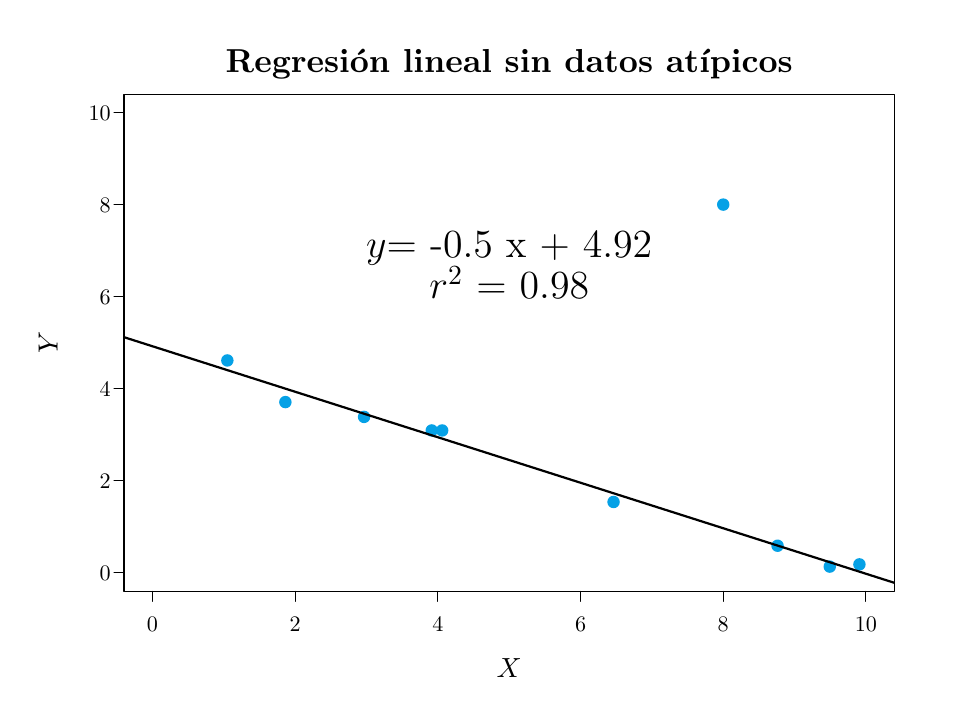
\begin{tikzpicture}[x=1pt,y=1pt]
\definecolor{fillColor}{RGB}{255,255,255}
\path[use as bounding box,fill=fillColor,fill opacity=0.00] (0,0) rectangle (325.21,238.49);
\begin{scope}
\path[clip] ( 34.80, 34.80) rectangle (313.21,214.49);
\definecolor{fillColor}{RGB}{5,161,230}

\path[fill=fillColor] ( 72.15,118.24) circle (  2.25);

\path[fill=fillColor] (270.97, 51.29) circle (  2.25);

\path[fill=fillColor] ( 93.12,103.19) circle (  2.25);

\path[fill=fillColor] (146.01, 92.94) circle (  2.25);

\path[fill=fillColor] (211.70, 67.10) circle (  2.25);

\path[fill=fillColor] (149.78, 92.94) circle (  2.25);

\path[fill=fillColor] (289.83, 43.74) circle (  2.25);

\path[fill=fillColor] (300.55, 44.55) circle (  2.25);

\path[fill=fillColor] (121.56, 97.84) circle (  2.25);
\end{scope}
\begin{scope}
\path[clip] (  0.00,  0.00) rectangle (325.21,238.49);
\definecolor{drawColor}{RGB}{0,0,0}

\path[draw=drawColor,line width= 0.4pt,line join=round,line cap=round] ( 45.11, 34.80) -- (302.90, 34.80);

\path[draw=drawColor,line width= 0.4pt,line join=round,line cap=round] ( 45.11, 34.80) -- ( 45.11, 31.21);

\path[draw=drawColor,line width= 0.4pt,line join=round,line cap=round] ( 96.67, 34.80) -- ( 96.67, 31.21);

\path[draw=drawColor,line width= 0.4pt,line join=round,line cap=round] (148.23, 34.80) -- (148.23, 31.21);

\path[draw=drawColor,line width= 0.4pt,line join=round,line cap=round] (199.79, 34.80) -- (199.79, 31.21);

\path[draw=drawColor,line width= 0.4pt,line join=round,line cap=round] (251.34, 34.80) -- (251.34, 31.21);

\path[draw=drawColor,line width= 0.4pt,line join=round,line cap=round] (302.90, 34.80) -- (302.90, 31.21);

\node[text=drawColor,anchor=base,inner sep=0pt, outer sep=0pt, scale=  0.80] at ( 45.11, 20.40) {0};

\node[text=drawColor,anchor=base,inner sep=0pt, outer sep=0pt, scale=  0.80] at ( 96.67, 20.40) {2};

\node[text=drawColor,anchor=base,inner sep=0pt, outer sep=0pt, scale=  0.80] at (148.23, 20.40) {4};

\node[text=drawColor,anchor=base,inner sep=0pt, outer sep=0pt, scale=  0.80] at (199.79, 20.40) {6};

\node[text=drawColor,anchor=base,inner sep=0pt, outer sep=0pt, scale=  0.80] at (251.34, 20.40) {8};

\node[text=drawColor,anchor=base,inner sep=0pt, outer sep=0pt, scale=  0.80] at (302.90, 20.40) {10};

\path[draw=drawColor,line width= 0.4pt,line join=round,line cap=round] ( 34.80, 41.46) -- ( 34.80,207.84);

\path[draw=drawColor,line width= 0.4pt,line join=round,line cap=round] ( 34.80, 41.46) -- ( 31.21, 41.46);

\path[draw=drawColor,line width= 0.4pt,line join=round,line cap=round] ( 34.80, 74.73) -- ( 31.21, 74.73);

\path[draw=drawColor,line width= 0.4pt,line join=round,line cap=round] ( 34.80,108.01) -- ( 31.21,108.01);

\path[draw=drawColor,line width= 0.4pt,line join=round,line cap=round] ( 34.80,141.28) -- ( 31.21,141.28);

\path[draw=drawColor,line width= 0.4pt,line join=round,line cap=round] ( 34.80,174.56) -- ( 31.21,174.56);

\path[draw=drawColor,line width= 0.4pt,line join=round,line cap=round] ( 34.80,207.84) -- ( 31.21,207.84);

\node[text=drawColor,anchor=base east,inner sep=0pt, outer sep=0pt, scale=  0.80] at ( 30.00, 38.70) {0};

\node[text=drawColor,anchor=base east,inner sep=0pt, outer sep=0pt, scale=  0.80] at ( 30.00, 71.98) {2};

\node[text=drawColor,anchor=base east,inner sep=0pt, outer sep=0pt, scale=  0.80] at ( 30.00,105.25) {4};

\node[text=drawColor,anchor=base east,inner sep=0pt, outer sep=0pt, scale=  0.80] at ( 30.00,138.53) {6};

\node[text=drawColor,anchor=base east,inner sep=0pt, outer sep=0pt, scale=  0.80] at ( 30.00,171.80) {8};

\node[text=drawColor,anchor=base east,inner sep=0pt, outer sep=0pt, scale=  0.80] at ( 30.00,205.08) {10};

\path[draw=drawColor,line width= 0.4pt,line join=round,line cap=round] ( 34.80, 34.80) --
	(313.21, 34.80) --
	(313.21,214.49) --
	( 34.80,214.49) --
	( 34.80, 34.80);
\end{scope}
\begin{scope}
\path[clip] (  0.00,  0.00) rectangle (325.21,238.49);
\definecolor{drawColor}{RGB}{0,0,0}

\node[text=drawColor,anchor=base,inner sep=0pt, outer sep=0pt, scale=  1.20] at (174.01,222.30) {\bfseries Regresión lineal sin datos atípicos};

\node[text=drawColor,anchor=base,inner sep=0pt, outer sep=0pt, scale=  1.00] at (174.01,  3.60) {$X$};

\node[text=drawColor,rotate= 90.00,anchor=base,inner sep=0pt, outer sep=0pt, scale=  1.00] at ( 10.80,124.65) {$Y$};
\end{scope}
\begin{scope}
\path[clip] ( 34.80, 34.80) rectangle (313.21,214.49);
\definecolor{fillColor}{RGB}{5,161,230}

\path[fill=fillColor] (251.34,174.56) circle (  2.25);
\definecolor{drawColor}{RGB}{0,0,0}

\path[draw=drawColor,line width= 0.8pt,line join=round,line cap=round] ( 34.80,126.65) -- (313.21, 37.88);

\node[text=drawColor,anchor=base,inner sep=0pt, outer sep=0pt, scale=  1.00] at (174.01,155.42) {\Large $y$= -0.5 x + 4.92};

\node[text=drawColor,anchor=base,inner sep=0pt, outer sep=0pt, scale=  1.00] at (174.01,140.45) {\Large $r^2$ = 0.98};
\end{scope}
\end{tikzpicture}
}
\end{center}

\note{Los datos atípicos en un estudio de regresión son un problema porque suelen provocar cambios drásticos en el modelo de regresión.

Como puede apreciarse en estos dos diagramas de dispersión, hay una clara tendencia lineal de la nube de puntos, pero en el primer caso hay
un dato atípico. Si se calcula la recta de regresión con el dato atípico, la recta resultante aparece bastante desviada de la tendencia de
la nube de puntos ya que el dato atípico está ejerciendo una gran influencia sobre ella. Como consecuencia el modelo resultante tiene
coeficiente de determinación $0.08$ y lo que indica que esta recta no explica bien la relación entre las variables. Sin embargo, cuando se
calcula la recta sin tener en cuenta el dato atípico, la recta resultante tiene un coeficiente de determinación de $0.98$ y explica casi a
la perfección la relación que hay entre las variables. 

Así pues, cuando haya datos atípicos en un estudio de regresión habrá que tener mucho cuidado con ellos y muchas ocasiones se eliminarán
para que no distorsionen el modelo de regresión.}
\end{frame}


\subsection{Medidas de relación entre atributos}
%---------------------------------------------------------------------slide----
\begin{frame}
\frametitle{Relaciones entre atributos}
Los modelos de regresión vistos sólo pueden aplicarse cuando las variables estudiadas son cuantitativas.

Cuando se desea estudiar la relación entre atributos, tanto ordinales como nominales, es necesario recurrir a otro tipo
de medidas de relación o de asociación. En este tema veremos tres de ellas:
\begin{itemize}
\item Coeficiente de correlación de Spearman.
\item Coeficiente chi-cuadrado.
\item Coeficiente de contingencia.
\end{itemize}

\note{La regresión sólo tiene sentido cuando cuando las variables estudiadas son cuantitativas.

Cuando se desea estudiar la relación entre atributos, tanto ordinales como nominales, es necesario recurrir a otro tipo
de medidas de relación o de asociación. Veremos tres de las más importantes que son
\begin{itemize}
\item Coeficiente de correlación de Spearman.
\item Coeficiente chi-cuadrado.
\item Coeficiente de contingencia.
\end{itemize}
}
\end{frame}


%---------------------------------------------------------------------slide----
\begin{frame}
\frametitle{Coeficiente de correlación de Spearman}
Cuando se tengan atributos ordinales es posible ordenar sus categorías y asignarles valores ordinales, de manera que se
puede calcular el coeficiente de correlación lineal entre estos valores ordinales. 

Esta medida de relación entre el orden que ocupan las categorías de dos atributos ordinales se conoce como coeficiente
ce correlación de Spearman, y puede demostrarse fácilmente que puede calcularse a partir de la siguiente fórmula

\begin{definicion}[Coeficiente de correlación de Spearman]
Dada una muestra de $n$ individuos en los que se han medido dos atributos ordinales $X$ e $Y$, el coeficiente de
correlación de Spearman se define como: 
\[
r_s = 1-\frac{6\sum d_i^2}{n(n^2-1)}
\]
donde $d_i$ es la diferencia entre el valor ordinal de $X$ y el valor ordinal de $Y$ del individuo $i$.
\end{definicion}

\note{Si queremos estudiar la relación entre dos atributos ordinales, como sus categorías pueden ordenarse, una posibilidad tomar sus
valores de orden, que serían numéricos, y calcular el coeficiente de correlación lineal entre los órdenes.

Esta medida se conoce como coeficiente de correlación de Spearman, que se representa como $r_s$ y también puede calcularse haciendo la suma
de los cuadrados de las diferencias entre los números de orden del valor de $X$ e $Y$ en cada indiviudo, multiplicada por 6, dividida por el
tamaño de la muestra multiplicado por el cuadrado del tamaño de la muestra menos 1 y restando el resultado del cociente a 1.
}
\end{frame}


%---------------------------------------------------------------------slide----
\begin{frame}
\frametitle{Interpretación del coeficiente de correlación de Spearman}
Como el coeficiente de correlación de Spearman es en el fondo el coeficiente de correlación lineal aplicado a los
órdenes, se tiene:
\[
-1\leq r_s\leq 1,
\]
de manera que:
\begin{itemize}
\item Si $r_s=0$ entonces no existe relación entre los atributos ordinales.
\item Si $r_s=1$ entonces los órdenes de los atributos coinciden y existe una relación directa perfercta.
\item Si $r_s=-1$ entonces los órdenes de los atributos están invertidos y existe una relación inversa perfecta.
\end{itemize}
En general, cuanto más cerca de $1$ o $-1$ esté $r_s$, mayor será la relación entre los atributos, y cuanto más cerca
de $0$, menor será la relación.

\note{Como el coeficiente de correlación de Spearman es en el fondo el coeficiente de correlación lineal aplicado a los
órdenes, su valor estará entre -1 y 1 y se interpreta de manera similar al coeficiente de correlación lineal, es decir,
\begin{itemize}
\item Si $r_s=0$ entonces no existe relación entre los atributos ordinales.
\item Si $r_s=1$ entonces los órdenes de los atributos coinciden y existe una relación directa perfercta.
\item Si $r_s=-1$ entonces los órdenes de los atributos están invertidos y existe una relación inversa perfecta.
\end{itemize}
}
\end{frame}


%---------------------------------------------------------------------slide----
\begin{frame}
\frametitle{Cálculo del coeficiente de correlación de Spearman}
\framesubtitle{Ejemplo}
Una muestra de 5 alumnos realizaron dos tareas diferentes $X$ e $Y$, y se ordenaron de acuerdo a la destreza que
manifestaron en cada tarea:
\[
\begin{array}{lrrrr}
\hline
\text{Alumnos} & X & Y & d_i & d_i^2\\
\hline
\text{Alumno 1} & 2 & 3 & -1 & 1\\
\text{Alumno 2} & 5 & 4 & 1 & 1 \\
\text{Alumno 3} & 1 & 2 & -1 & 1\\
\text{Alumno 4} & 3 & 1 & 2 & 4\\
\text{Alumno 5} & 4 & 5 & -1 & 1\\
\hline
\sum &  &  & 0 & 8 \\
\hline
\end{array}
\]
El coeficiente de correlación de Spearman para esta muestra es 
\[
r_s = 1-\frac{6\sum d_i^2}{n(n^2-1)} = 1- \frac{6\cdot 8}{5(5^2-1)} = 0.6,
\]
lo que indica que existe bastante relación directa entre las destrezas manifestadas en ambas tareas.

\note{Para ilustrar el cálculo del coeficiente de correlación de Spearman, supongamos una muestra de 5 alumnos que realizaron dos tareas
diferentes $X$ e $Y$, y se ordenaron de acuerdo a la destreza que manifestaron en cada tarea.

El primer alumno fue el segundo con más destreza en la tarea $X$ y el tercero en la tarea $Y$ de manera que la diferencia entre los órdenes
en $X$ e $Y$ es $-1$ y su cuadrado vale 1. El segundo alumno fue el peor en la tarea $X$ y el penúltimo en la tarea $Y$ de manera que la
diferencia entre sus órdenes en $X$ e $Y$ vale también $-1$ y su cuadrado 1, etc.  

Una vez calculados los cuadrados de las diferencias entre los órdenes, se suman, se multiplican por 6 y se dividen por el cuadrado del
tamaño de la muestra, que vale 5,  por el cuadrado del tamaño de la muestra menos, que es $5^2-1$ y finalmente el resultado del cociente se
resta a 1. Esto nos da un coeficiente de correlación de Spearman de 0.6, lo cual indica que existe bastante relación directa entre las
destrezas manifestadas en ambas tareas.
}
\end{frame}


%---------------------------------------------------------------------slide----
\begin{frame}
\frametitle{Cálculo del coeficiente de correlación de Spearman}
\framesubtitle{Ejemplo con empates}
Cuando hay empates en el orden de las categorías se atribuye a cada valor empatado la media aritmética de los valores
ordinales que hubieran ocupado esos individuos en caso de no haber estado empatados.

Si en el ejemplo anterior los alumnos 4 y 5 se hubiesen comportado igual en la primera tarea y los alumnos 3 y 4 se
hubiesen comportado igual en la segunda tarea, entonces se tendría
\[
\begin{array}{lrrrr}
\hline
\text{Alumnos} & X & Y & d_i & d_i^2\\
\hline
\text{Alumno 1} & 2 & 3 & -1 & 1\\
\text{Alumno 2} & 5 & 4 & 1 & 1 \\
\text{Alumno 3} & 1 & 1.5 & -0.5 & 0.25\\
\text{Alumno 4} & 3.5 & 1.5 & 2 & 4\\
\text{Alumno 5} & 3.5 & 5 & -1.5 & 2.25\\
\hline
\sum &  &  & 0 & 8.5 \\
\hline
\end{array}
\]
El coeficiente de correlación de Spearman para esta muestra es 
\[
r_s = 1-\frac{6\sum d_i^2}{n(n^2-1)} = 1- \frac{6\cdot 8.5}{5(5^2-1)} = 0.58.
\]

\note{Cuando haya individuos con la misma categoría del atributo, entonces dichos individuos recibirán el mismo número de orden y de manera
que habrá empates en el orden. En tal caso se atribuye a cada valor empatado la media aritmética de los valores ordinales que hubieran
ocupado esos individuos en caso de no haber estado empatados.

Si en ejemplo anterior los alumnos 4 y 5 se hubiesen comportado igual en la primera tarea, entonces como ambos ocupan la posición 3 y 4
en la ordenación, se toma la media $3.5$ y se le asigna dicho valor a ambos. Del mismo modo, si los alumnos 3 y 4 se hubiesen comportado
igual en la segunda tarea, como el orden que ocupan es el primero y el segundo, entonces a ambos se le asigna la media $1.5$.

El resto de los cálculos para el coeficiente de Spearman se haría igual que en el caso en que no había empates.
}
\end{frame}


%---------------------------------------------------------------------slide----
\begin{frame}
\frametitle{Relación entre atributos nominales}
Cuando se quiere estudiar la relación entre atributos nominales no tiene sentido calcular el coeficiente de correlación
de Spearman ya que las categorías no pueden ordenarse.

Para estudiar la relación entre atributos nominales se utilizan medidas basadas en las frecuencias de la tabla de
frecuencias bidimensional, que para atributos se suele llamar \emph{tabla de contingencia}.

\structure{\textbf{Ejemplo}} En un estudio para ver si existe relación entre el sexo y el hábito de fumar se ha tomado
una muestra de 100 personas.
La tabla de contingencia resultante es
\[
\begin{array}{|l|rr|r|} 
\hline
\text{Sexo}\backslash\text{Fuma} & \text{Si} & \text{No} & n_i\\
\hline
\text{Mujer} & 12 & 28 & 40 \\
\text{Hombre} & 26 & 34 & 60 \\
\hline
n_j & 38 & 62 & 100\\
\hline
\end{array}
\]
Si el hábito de fumar fuese independiente del sexo, la proporción de fumadores en mujeres y hombres sería la misma.

\note{Cuando se quiere estudiar la relación entre atributos nominales no tiene sentido calcular el coeficiente de correlación
de Spearman ya que las categorías no pueden ordenarse. En este caso se utilizan medidas basadas en las frecuencias de la tabla de
frecuencias bidimensional, que para atributos se suele llamar \emph{tabla de contingencia}.

En este ejemplo tenemos una tabla de contingencia para los atributos sexo y hábito de fumar, ambos nominales. En la muestra hay 12 mujeres
fumadoras, 28 no fumadoras, 26 hombres fumadores y 34 no fumadores. En total tenemos una muestra de tamaño 100. 

La forma de estudiar la relación entre el sexo y el hábito de fumar es por medio de las frecuencias relativas de cada par de categorías.
Así, si el hábito de fumar fuese independiente del sexo, la proporción de fumadores en mujeres y hombres sería la misma, mientras que si
hubiese dependencia, serían significativamente diferentes.
}
\end{frame}


%---------------------------------------------------------------------slide----
\begin{frame}
\frametitle{Frecuencias teóricas o esperadas}
En general, dada una tabla de contingencia para dos atributos $X$ e $Y$, 
\[
\begin{array}{|c|ccccc|c|}
\hline
X\backslash Y & y_1 & \cdots & y_j & \cdots & y_q & n_x\\
\hline
x_1 & n_{11} & \cdots & n_{1j} & \cdots & n_{1q} & n_{x_1}\\
\vdots & \vdots & \ddots & \vdots & \ddots & \vdots & \vdots \\
x_i & n_{i1} & \cdots & n_{ij} & \cdots & n_{iq} & n_{x_i}\\
\vdots & \vdots & \ddots & \vdots & \ddots & \vdots & \vdots\\
x_p & n_{p1} & \cdots & n_{pj} & \cdots & n_{pq} & n_{x_p} \\
\hline
n_y & n_{y_1} & \cdots & n_{y_j} & \cdots & n_{y_q} & n\\
\hline
\end{array}
\]
si $X$ e $Y$ fuesen independientes, para cualquier valor $y_j$ se tendría
\[
\frac{n_{1j}}{n_{x_1}} = \frac{n_{2j}}{n_{x_2}} = \cdots = \frac{n_{pj}}{n_{x_p}} = \frac{n_{1j}+\cdots
+n_{pj}}{n_{x_1}+\cdots+n_{x_p}} = \frac{n_{y_j}}{n},
\]
de donde se deduce que
\[
n_{ij} = \frac{n_{x_i}n_{y_j}}{n}.
\]

A esta última expresión se le llama \emph{frecuencia teórica} o \emph{frecuencia esperada} del par $(x_i,y_j)$. 

\note{En general, dada una tabla de contingencia pra dos atributos $X$ e $Y$, si las variables fuesen independientes, entonces la proporción
de individuos que presentan el valor $y_j$ en la variable $Y$ entre los que presentan el valor $x_1$ en la variable $X$ sería la frecuencia
absoluta del par $(x_i,y_j)$ $n_{ij}$ divida entre la frecuencia absoluta de $x_1$ y esta frecuencia sería la misma que la proporción de
individuos con el valor $y_j$ en $Y$ entre los que presentan el valor $x_2$ en $X$, y en general, al ser independiente de $X$ sería la misma
para cualquier otra categoría de $X$, de manera que todas serían iguales a la proporción total de individuos en la muestra con valor $y_j$
en la variable $Y$, que se obtendría dividiendo la frecuencia absoluta de $y_j$ entre el tamaño de la muestra.

De esta igualdad se puede deducir que la frecuencia absoluta de cualquier par $(x_i,y_j)$ se podría calcular multiplicando las frecuencias
absolutas de $x_i$, $n_i$ y $y_j$ que es $n_j$ y dividendo por el tamaño de la muestra.

A estas frecuencias calculadas bajo la hipótesis de independencia, se les llama \emph{frecuencia teóricas} o \emph{frecuencia esperadas}.
}
\end{frame}


%---------------------------------------------------------------------slide----
\begin{frame}
\frametitle{Coeficiente chi-cuadrado $\chi^2$}
Es posible estudiar la relación entre dos atributos $X$ e $Y$ comparando las frecuencias reales con las esperadas:
\begin{definicion}[Coeficiente chi-cuadrado $\chi^2$]
Dada una muestra de tamaño $n$ en la que se han medido dos atributos $X$ e $Y$, se define el coeficiente $\chi^2$ como
\[
\chi^2 = \sum_{i=1}^p\sum_{j=1}^q \frac{\left(n_{ij}-\frac{n_{x_i}n_{y_j}}{n}\right)^2}{\frac{n_{x_i}n_{y_j}}{n}},
\]
donde $p$ es el número de categorías de $X$ y $q$ el número de categorías de $Y$.
\end{definicion}

Por ser suma de cuadrados, se cumple que 
\[
\chi^2 \geq 0,
\]
de manera que $\chi^2=0$ cuando los atributos son independientes, y crece a medida que aumenta la dependencia entre las variables.

\note{Una posible forma de estudiar la relación entre dos atributos nominales es comparar sus frecuencias absolutas reales con las esperadas
bajo la hipótesis de indepencia. Esto es precisamente lo que hace un estadístico conocido como coeficiente chi-cuadrado, que se denota con
la letra griega $\chi^2$ y se calcula sumando para cada par de la variable bidimensional los cuadrados de las diferencias entre las
frecuencias reales y las frecuencias esperadas, dividos por las propias frecuencias esperadas.

Como se trata de una suma de cuadrados, el coeficiente chi-cuadrado siempre es positivo. Cuando los atributos sean independientes, las
frecuencias reales coincidirán con las esperadas y todos los sumandos se anularán, de manera que el coeficiente chi-cuadrado valdrá cero. Y
en la medida que cada vez haya más dependencia, las diferencias entre las frecuencias reales y las esperadas serán cada vez mayores de forma
que el coeficiente chi-cuadrado será también mayor.
}
\end{frame}


%---------------------------------------------------------------------slide----
\begin{frame}
\frametitle{Cálculo del coeficiente chi-cuadrado $\chi^2$}
\framesubtitle{Ejemplo}
Siguiendo con el ejemplo anterior, a partir de la tabla de contingencia 
\[
\begin{array}{|l|rr|r|} 
\hline
\text{Sexo}\backslash\text{Fuma} & \text{Si} & \text{No} & n_i\\
\hline
\text{Mujer} & 12 & 28 & 40 \\
\text{Hombre} & 26 & 34 & 60 \\
\hline
n_j & 38 & 62 & 100\\
\hline
\end{array}
\]
se obtienen las siguientes frecuencias esperadas:
\[
\renewcommand{\arraystretch}{1.5}
\begin{array}{|l|rr|r|} 
\hline
\mbox{Sexo$\backslash$Fuma} & \mbox{Si} & \mbox{No} & n_i\\
\hline
\text{Mujer} & \frac{40\cdot 38}{100}=15.2 & \frac{40\cdot 62}{100}=24.8 & 40 \\
\text{Hombre} & \frac{60\cdot 38}{100}=22.8 & \frac{60\cdot 62}{100}=37.2 & 60 \\
\hline
n_j & 38 & 62 & 100\\
\hline
\end{array}
\]
y el coeficiente $\chi^2$ vale
\[
\chi^2 = \frac{(12-15.2)^2}{15.2}+\frac{(28-24.8)^2}{24.8}+\frac{(26-22.8)^2}{22.8}+\frac{(34-37.2)^2}{37.2} = 1.81,
\]
lo que indica que no existe gran relación entre el sexo y el hábito de fumar.

\note{Siguiendo con el ejemplo del sexo y el hábito de fumar, a partir de la tabla de contingencia se calculan las frecuencias esperadas de
cada par. La frecuencia esperada de mujeres fumadoras es el número de mujeres 40, por el número de personas fumadoras 38, dividido por el
tamaño de la muestra 100, lo que da $15.2$. Etc. 

Una vez calculadas las frecuencias esperadas, para calcular el coeficiente chi-cuadrado vamos calculando los cuadrados de las diferencias
entre las frecuencias reales y las esperadas, es decir, para las mujeres fumadoras sería $(12-15.2)^2$ y esto se divide por la frecuencia
esperada $15.2$. Del mismo modo se calculan los sumandos para el resto de los pares y se realiza la suma, lo que nos da un coeficiente
chi-cuadrado de $1.81$, que al ser un valor próximo a 0 indica que no hay gran relación entre el sexo y el hábito de fumar.
}
\end{frame}


%---------------------------------------------------------------------slide----
\begin{frame}
\frametitle{Coeficiente de contingencia}
El coeficiente $\chi^2$ depende del tamaño muestral, ya que al multiplicar por una constante las frecuencias de todas
las casillas, su valor queda multiplicado por dicha constante, lo que podría llevarnos al equívoco de pensar que ha
aumentado la relación, incluso cuando las proporciones se mantienen.
En consecuencia el valor de $\chi^2$ no está acotado superiormente y resulta difícil de interpretar.

Para evitar estos problemas se suele utilizar el siguiente estadístico:
\begin{definicion}[Coeficiente de contingencia]
Dada una muestra de tamaño $n$ en la que se han medido dos atributos $X$ e $Y$, se define el \emph{coeficiente de
contingencia} como 
\[
C = \sqrt{\frac{\chi^2}{\chi^2+n}}
\]
\end{definicion}

\note{El principal problema del coeficiente chi-cuadrado es que depende del tamaño muestral ya que se calcula a partir de las frecuencias
absolutas, no de las relativas. De hecho, se puede comprobar que al multiplicar por una constante las frecuencias de todas
las casillas de la tabla de contingencia, su valor queda multiplicado por dicha constante, lo que podría llevarnos al equívoco de pensar que
ha aumentado la relación, incluso cuando las proporciones se mantienen. En consecuencia el valor de $\chi^2$ no está acotado superiormente y
resulta difícil de interpretar.

Para evitar estos problemas suele utilizarse otro estadístico conocido como coeficiente de contingencia, que se denota $C$, y se calcula a
partir del coeficiente chi-cuadrado haciendo la raíz del cociente entre el coeficiente-chi cuadrado entre el mismo coeficiente chi-cuadrado
mas el tamaño de la muestra.
}
\end{frame}


%---------------------------------------------------------------------slide----
\begin{frame}
\frametitle{Interpretación del coeficiente de contingencia}
De la definición anterior se deduce que 
\[
0\leq C\leq 1,
\]
de manera que cuando $C=0$ las variables son independientes, y crece a medida que aumenta la relación.

Aunque $C$ nunca puede llegar a valer 1, se puede demostrar que para tablas de contingencia con $k$ filas y $k$
columnas, el valor máximo que puede alcanzar $C$ es $\sqrt{(k-1)/k}$.

\structure{\textbf{Ejemplo}} En el ejemplo anterior el coeficiente de contingencia vale
\[
C = \sqrt{\frac{1.81}{1.81+100}} = 0.13.
\]
Como se trata de una tabla de contingencia de $2\times 2$, el valor máximo que podría tomar el coeficiente de
contingencia es $\sqrt{(2-1)/2}=\sqrt{1/2}=0.707$, y como $0.13$ está bastante lejos de este valor, se puede concluir
que no existe demasiada relación entre el hábito de fumar y el sexo.

\note{De la definición del coeficiente de contingencia es fácil ver que, al ser el numerador siempre menor que el denominador, siempre
estará entre 0 y 1, de manera que el coeficiente de contingencia será nulo cuando las variables sean independientes, y estará más próximo a
1 a medida que aumente la dependencia.

Aunque el coeficiente de contingencia nunca puede llegar a valer 1, se puede demostrar que para tablas de contingencia con $k$ filas y $k$
columnas, el valor máximo que puede alcanzar es $\sqrt{(k-1)/k}$, de modo que se puede comparar con este valor.

En el ejemplo del sexo y el hábito de fumar, como el coeficiente chi-cuadrado valía $1.81$, el coeficiente de contingencia vale la
raíz cuadrada de $1.81$ dividido entre $1.81$ más el tamaño de la muestra 100, lo que da $0.13$. Y como se trata de una tabla de
contingencia de $2\times 2$, el valor máximo que podría tomar el coeficiente de contingencia es $\sqrt{(2-1)/2}=\sqrt{1/2}=0.707$, y como
$0.13$ está bastante lejos de este valor, se puede concluir que no existe demasiada relación entre el hábito de fumar y el sexo.
}
\end{frame}
